%Python
%-----------------------------
%---- Präambel/Preamble ------
%-----------------------------

\documentclass[	a4paper,
				11pt,
				%DIV=11,
				%bigheadings,
				%idxtotoc,
				%listof=totoc,	
				%bibtotoc,		
				%halfparskip,
				%cleardoubleempty,
				%openright,
				oneside]{scrartcl}
%-----------------------------

%\usepackage[ngerman]{babel}
\usepackage[T1]{fontenc}
\usepackage[utf8]{inputenc}
\usepackage{comment}

\usepackage{graphicx}						
\usepackage{float}
\usepackage{wrapfig}
% \usepackage{subfigure}
\usepackage{caption}
\usepackage{subcaption}

\usepackage{geometry}						% For "newgeometry" on title page
\geometry{a4paper,left=30mm,right=20mm}

\usepackage{blindtext}
\usepackage{layout}

\PassOptionsToPackage{hyphens}{url}		
\usepackage[pdfborder={0 0 0},
			colorlinks=true, 
			linkcolor=black,
			citecolor=red,
			]{hyperref}
			
\usepackage[numbers]{natbib}				

\usepackage{pdfpages}

\usepackage{color}
\usepackage{xcolor}

\usepackage{setspace}

\usepackage{longtable}
\usepackage{multirow}
\usepackage{colortbl}

% \usepackage{subcaption}
\usepackage{hyperref}

% Optional: to make the caption labels more descriptive
% \captionsetup[subfigure]{labelformat=simple, labelsep=colon}
% \renewcommand{\thesubfigure}{Row \arabic{subfigure}}

%----Kopfzeile------------------------------------------------------------------------------------------------------------------------------------------------
\usepackage{scrlayer-scrpage} 
%\usepackage{scrpage2} 							% Aufruf KOMA-Skript für Kopfzeilen

\pagestyle{scrheadings}							% Definition der Eigenen Headerformatierung
\clearscrheadfoot 								% alle Standard-Werte und Formatierungen raus
%\automark[chapter]{section}						% Kapitel und Section als Inhalt der Variablen leftmark und rightmark
\ohead{\pagemark}								% Seitenzahl auf äußerem Rand
\ihead{\ifthispageodd{\leftmark}{\rightmark}} 	% Innere Überschrift mit Kapitel bei linker Seite und Section bei rechter Seite -> geht nur in Verbindung mit
												% zweiseitigem Text wirklich sinnvoll
\setheadsepline{0.4pt} 							% Trennlinie Fußzeile und Textkörper
\setkomafont{pagehead}{\scshape}				% Schriftart in Kopfzeile, \scshape = Kapitelchen
%----Fußzeile-------------------------------------------------------------------------------------------------------------------------------------------------
\setfootsepline{0.4pt} 							% Trennlinie Fußzeile und Textkörper
\setkomafont{pagefoot}{\scshape}				% Schriftart in Fußfzeile, \scshape = Kapitelchen
\ifoot{\footnotesize{Gianluca Decaro}}
\ofoot{\footnotesize{Bachelor thesis}}		
%-------------------------------------------------------------------------------------------------------------------------------------------------------------

\defpagestyle{myPageStyle}{
	(0pt ,0pt)
	{\hfill\pagemark} {\hfill\pagemark} {\hfill\pagemark}
	(0pt ,0pt)	
}{
{
	(\textwidth ,0.4pt)
	\footnotesize{Gianluca Decaro} \hfill \footnotesize{Bachelor thesis}} {\footnotesize{Gianluca Decaro} \hfill \footnotesize{Bachelor thesis}} {\footnotesize{Gianluca Decaro} \hfill \footnotesize{Bachelor thesis}}
	(0pt ,0pt)
}


%----Farbdefinition--THI-Blau-------------------------------------------------------------------------
\definecolor{haw_mag}{rgb}{0,0.112,0.47}
\addtokomafont{section}{\color{haw_mag} \rmfamily \scshape} 
\addtokomafont{subsection}{\color{haw_mag} \rmfamily}
\addtokomafont{subsubsection}{\color{haw_mag} \rmfamily}
\addtokomafont{paragraph}{\color{haw_mag} \rmfamily}
\addtokomafont{subparagraph}{\rmfamily}

\usepackage{mathpazo}
\usepackage{domitian}
\usepackage[T1]{fontenc}
\let\oldstylenums\oldstyle
%-------------------------------------------------------------------------------------------------------------------------------------------------------------

\definecolor{tab_2}{RGB}{230,230,230}
\definecolor{tab_1}{RGB}{85,128,214}

%------Längenanpassung----------------------------------------------------------------------------------------------------------------------------------------
\setlength{\headsep}{10mm}						% Textabstand zur Kopfzeile
\setlength{\footskip}{15mm}						% Abstand zur Fußzeile
\setlength{\textheight}{235mm}					% Texthöhe
%-------------------------------------------------------------------------------------------------------------------------------------------------------------


%----Glossar--------------------------------------------------------------------------------------------------------------------------------------------------
\usepackage[toc]{glossaries} 			
\makeglossaries

%----------Glossar/Glossary-------------------------------------------------------------
% Anzeige erst auf Tools>Glossary bei jeder Änderung!!
\newglossaryentry{HVI}{name={HVI},description={Human-Vehicle Interaction}} 
\newglossaryentry{HAD}{name={HAD},description={Highly automated driving}} 
\newglossaryentry{DDT}{name={DDT},description={Dynamic Driving Task}} 
\newglossaryentry{ODD}{name={ODD},description={Operational design domains}} 
\newglossaryentry{NDRA}{name={NDRA},description={Non-Driving Related Activities}} 
\newglossaryentry{NDRT}{name={NDRT},description={Non-Driving Related Tasks}} 
\newglossaryentry{UI}{name={UI},description={User Interface}} 
\newglossaryentry{HMI}{name={HMI},description={Human-Machine Interaction}} 
\newglossaryentry{AV}{name={AV},description={Automated Vehicle}} 
\newglossaryentry{RV}{name={RV},description={Recreational Vehicle}} 
\newglossaryentry{UX}{name={UX},description={User Experience}} 
\newglossaryentry{HUD}{name={HUD},description={Head-Up Display}} 
\newglossaryentry{HDD}{name={HDD},description={Head-Down Display}} 
\newglossaryentry{VUI}{name={VUI},description={Voice User Interface}} 
\newglossaryentry{WSD}{name={WSD},description={Windshield Display}} 
\newglossaryentry{AR}{name={AR},description={Augmented Reality}} 
\newglossaryentry{2D}{name={2D},description={Two-Dimensional}} 
\newglossaryentry{ADS}{name={ADS},description={Automated Driving System}} 
\newglossaryentry{HCD}{name={HCD},description={Human-Centered Design}} 
\newglossaryentry{IVIS}{name={IVIS},description={In-Vehicle Infotainment Systems}} 
\newglossaryentry{GUI}{name={GUI},description={Graphical User Interface}} 
\newglossaryentry{POI}{name={POI},description={Point of Interest}} 
\newglossaryentry{NUI}{name={NUI},description={Natural User Interface}} 
\newglossaryentry{ANOVA}{name={ANOVA},description={Analysis of Variance}} 
\newglossaryentry{SUS}{name={SUS},description={System Usability Score}} 
\newglossaryentry{UEQ}{name={UEQ},description={User Experience Questionnaire}} 
\newglossaryentry{QUESI}{name={QUESI},description={Questionnaire for the Subjective Consequence of Intuitive Use}} 
\newglossaryentry{meCUE}{name={meCUE},description={Modular Evaluation of Key Components of User Experience}} 
\newglossaryentry{MDF}{name={MDF},description={Medium Density Fiberboard}} 
\newglossaryentry{IV}{name={IV},description={Independent Variable}}
\newglossaryentry{DV}{name={DV},description={Dependent Variable}} 
					
%-------------------------------------------------------------------------------------------------------------------------------------------------------------

\includeonly{	
	titlepage,							
	affidavit,
	acknowledgments,
	abstractEN,
        % abstractDE,
        NoteOnAI,
	glossary,
	mainpart,
	%outlook,
	%fazit,
	appendices
	}
	
			
%-----------------------------
%------ BEGIN DOCUMENT -------
%-----------------------------

\begin{document}
	
	%----Vermeidung von Hurenkindern und Schusterjungen---------------------
	\widowpenalty=10000
	\clubpenalty=10000
	\displaywidowpenalty=10000	
	%-----------------------------------------------------------------------

    %---- Add spacing between paragraphs and disable indent ----
    \setlength{\parskip}{0.75em}
    \setlength{\parindent}{0pt}

	%Titelseite/title page	
	%----------Titelseite-------------------------------------------------------------

\newgeometry{textheight=0.9\paperheight, textwidth=0.76\paperwidth, left=30mm, right=20mm}

\begin{titlepage}	
	%----THI-Bertrandt-logo--------------------------------------------------------
		\begin{figure}[!h]
			\centering
			\includegraphics[width={0.4\textwidth}]{images/thiRGB.jpg}	
		\end{figure}																			
	%------------------------------------------------------------------------------
	
	\begin{center}
		\hrulefill 
	\end{center}
	
	
	\begin{center}	
		\vspace{1cm}
		
		\huge\textbf{
			Bachelor Thesis % oder Bachelor Thesis/Bachelorarbeit
			}\\[2.5em]
		\normalsize
			in the Degree Program Bachelor User Experience Design (UXD) \\
			%im Studiengang User Experience Design (UXD) \\
			Faculty Computer Science \\ [7em]
			%Fakultät Informatik \\ [7em]
	
		\Large\textbf{Designing Textile Interfaces for Automated Vehicles: Exploring Feedforward Cues for Intuitive yet Engaging Interactions.}	 \\ 

	\end{center}

	\vfill
	
 	% GERMAN VERSION
 	\begin{tabular}{ll}
 		First and last name:  & \textbf{Gianluca Decaro} 	\\ [3em]
		
 		Issuing date:	& 29.04.2025	\\ [1em] % issuing date
 		Date of hand-in:	& 04.08.2025	\\ [3em] %date of hand in
		
 		First Supervisor: 	& Prof. Veronika Ritzer	\\ [1em]
 		Second Supervisor: 	& Prof. Priv.-Doz. Dr. Andreas Riener	\\[3em]
		
 		%Firmenbetreuer:	& Dr. Sandro Hess \\ %if applicable
 	\end{tabular}
	    
    % ENGLISH VERSION
    
    %COMMENT
    \begin{comment}
	    \begin{tabular}{ll}
    		First and last name: & \textbf{Firstname Lastname}	\\ [3em]
    		
    		Issuing date:   	& xx.yy.zzzz	\\ [1em] % issuing date
    		Date of hand-in:	& xx.yy.zzzz	\\ [3em] %date of hand in
    		
    		First Supervisor: 	& Prof. Priv.-Doz. Dr. techn.Andreas Riener	\\ [1em]
    		Second Supervisor: 	& Prof. Dr. Firstname Lastname	\\[3em]
    		
    		Company Advisor:	& Dr. Firstname Lastname \\ %if applicable
	    \end{tabular}
	\end{comment}
	
\end{titlepage}

\restoregeometry					% include erzeugt immer eine neue Seite bei jedem Einbinden
	\cleardoublepage						% include always creates a new page
	
	\pagenumbering{Roman} 			% Römische Nummerierung der Kapitel/roman page numbering
	
	%Erklärung
	\thispagestyle{myPageStyle}
	%----------Eidesstattliche Erklärung/Affidavit---------------------------------------------------------------

\addsec{Affidavit}
%Ich erkläre hiermit, dass ich die Arbeit selbständig verfasst, noch nicht anderweitig für Prüfungszwecke vorgelegt, keine anderen als die angegebenen Quellen oder Hilfsmittel benützt sowie wörtliche und sinngemäße Zitate als solche gekennzeichnet habe.	\\[2em]

I hereby declare that this thesis is my own work, that I have not presented it elsewhere for examination purposes and that I have not used any sources or aids other than those stated. I have marked verbatim and indirect quotations as such. \\[2em]
	
Ingolstadt, \rule{0.3\textwidth}{0.4pt}	\\ [1.5cm]
	%\textcolor{white}{.}\qquad\qquad\qquad\qquad\quad \small (Datum) \\ [1.5cm]
	
%(Unterschrift) \\
Gianluca Decaro


	\cleardoublepage
	
	%Danksagung
	\thispagestyle{myPageStyle}
	%----------Danksagung/Acknowledgments--------------------------------------------------------------
\addsec{Acknowledgments}

I’d like to sincerely thank my supervisor, Professor Veronika Ritzer, for her patience and for the many insightful ideas that challenged and inspired me. Her support and feedback were crucial in shaping this work and keeping me motivated throughout my bachelor's thesis.

My deepest gratitude goes to my parents. Without their constant encouragement and support, pursuing my studies would not have been possible. Their belief in me, throughout my academic career and beyond, has meant everything.

And finally, a very special thank you to Sofia. Meeting her during my studies was a turning point, and I am so grateful for the life we’ve built together. Over the past few years, we’ve tackled countless challenges side by side, and her dedicated presence and support, especially during this thesis, have made an immeasurable difference.


% \blindtext
	\cleardoublepage
	
	
	%Kurzfassung/Abstract Englisch (for every thesis)
	\thispagestyle{myPageStyle}
	%----------Zusammenfassung Englisch/Abstract----------------------------------------------------------------
\addsec{Abstract}
% Here goes the English Abstract... 
% Abstract
% As automated vehicles transform car interiors into versatile living spaces, current human-machine interfaces, predominantly touchscreens, are becoming inadequate due to poor ergonomics, a lack of hedonic appeal, and their potential to induce motion sickness. Interactive electronic textiles (e-textiles) present a promising alternative, offering seamless integration and a richer tactile experience. However, their novelty poses a significant challenge: designing them to be intuitively understood and used by untrained, first-time users.

% This thesis investigates how different levels of feedforward cues can support intuitive yet engaging interactions with a novel HMI paradigm combining a shape-shifting e-textile interface on the center armrest with a windshield display for visual output. Following a human-centered design process, a high-fidelity prototype was developed and iteratively refined through a qualitative pre-study (n=5). A subsequent summative, between-subjects user study (n=30) quantitatively and qualitatively evaluated the performance, usability, and user experience of three distinct feedforward conditions: Inherent Cues (relying solely on the physical form), Augmented Light Cues (dynamic light projections on the textile), and Augmented Text Cues (explicit instructions on the windshield display).

% The results demonstrate that augmented feedforward is critical for the usability of a complex textile interface. Relying on inherent physical cues alone resulted in poor initial performance, significant usability issues, and a negative emotional response. In contrast, the Augmented Light Cues condition proved to be the superior solution, leading to significantly higher task success rates, fewer errors, and a more intuitive, usable, and emotionally positive user experience compared to both other conditions.

% These findings imply that for novel textile HMIs, the optimal user experience is achieved not by relying on physical form alone or explicit textual instruction, but through a balanced approach that enhances inherent physical properties with seamlessly integrated, non-verbal guidance. This work provides evidence for the high potential of the proposed HMI paradigm to create more ergonomic, safer, and hedonically rich in-vehicle experiences and offers concrete design recommendations for developing intuitive textile interfaces for future automated vehicles.


% ----


% As automated driving transforms vehicles into multifunctional living spaces, the need for new human-machine interfaces that are intuitive, engaging, and aesthetically aligned with a comfortable interior becomes paramount. Current touchscreen-dominated paradigms are ill-suited for this shift, creating ergonomic challenges and failing to provide a hedonically rich experience. Interactive electronic textiles (e-textiles) combined with windshield displays (WSDs) present a promising alternative, yet their novelty creates a significant learnability challenge for first-time users. This thesis addresses this gap by investigating how different levels of feedforward—cues that guide users before an action—can support intuitive, "walk-up-and-use" interactions with a non-wearable textile interface in an automotive context. Following a human-centered design process, a high-fidelity, shape-shifting textile prototype was developed for the vehicle's armrest, accompanied by a WSD. A between-subjects user study (n=30) was conducted to evaluate three feedforward conditions: a baseline with only the interface's inherent physical cues, a version augmented with abstract light projections on the textile, and a version with explicit text cues on the WSD. The results show that while a steep initial learning curve existed across all conditions, the augmented light cues significantly improved objective performance, perceived usability, and overall user experience, eliciting the most positive emotional response. Relying on inherent physical cues alone proved insufficient, leading to usability issues and user frustration, while remote text cues were less effective than integrated light due to cognitive load and discoverability issues. These findings demonstrate that for novel textile systems, integrated, non-verbal augmented feedforward is a prerequisite for creating a positive, intuitive, and engaging user experience. This work contributes empirically-grounded design recommendations, highlighting that the optimal approach balances inherent physical affordances with a seamlessly integrated layer of augmented guidance, thereby unlocking the full potential of textile interfaces for future vehicle interiors.


% ----


% As vehicle automation advances, the role of drivers shifts toward passive passengers, transforming car interiors into multifunctional living spaces. Traditional touchscreen-based interfaces, while widespread, are ill-suited for this new paradigm due to their reliance on visual attention and lack of tactile engagement. This thesis investigates how interactive, non-wearable textile surfaces, combined with windshield displays, can provide intuitive and emotionally engaging interaction experiences for passengers in automated vehicles. To explore this, a two-part study was conducted. A co-design pre-study (n=6) identified intuitive gestures and feedforward cues, which informed the development of a multimodal prototype combining tactile, abstract visual, and explicit textual feedforward. In the main user study (n=30), participants interacted with one of three interface versions, each representing a different level of feedforward. Quantitative data (e.g., success rates, SUS, UEQ, QUESI, meCUE) and qualitative feedback (e.g., interviews, observations) were collected to evaluate intuitiveness, user experience, and emotional engagement. Results show that while inherent feedforward supports intuitive use, combining it with abstract or explicit augmented cues significantly enhances user understanding and enjoyment. Participants favored playful, tactile elements and appreciated guidance that maintained a sense of autonomy. However, overly explicit cues occasionally disrupted the immersive experience. The findings suggest that carefully layered feedforward can balance usability and delight, making textile interfaces a promising HMI paradigm for future AVs. Limitations include the lab setting and use of Wizard-of-Oz techniques. Future work should explore long-term use and real-world integration to further assess feasibility and acceptance.


% ---- 


% As automated vehicles (AVs) transform car interiors into multifunctional living spaces, the need arises for novel human-machine interfaces (HMIs) that move beyond the ergonomic and experiential limitations of today's dominant touchscreen controls. This thesis explores how interactive e-textiles, combined with a windshield display (WSD), can offer a more intuitive, engaging, and seamlessly integrated alternative for passengers. The central research question investigates how different levels of feedforward can guide first-time, untrained users to interact with such a novel interface. Following a Quad-Diamond design process, a high-fidelity, shape-shifting textile prototype was developed and evaluated in a controlled lab study using a Wizard of Oz methodology. A between-subjects user study (N=30) compared three feedforward conditions: a baseline with only the interface's inherent physical cues, a version with augmented, on-surface light cues, and a version with augmented, textual cues on the WSD. The results from quantitative analysis of performance data and standardized questionnaires (SUS, UEQ, QUESI, meCUE), along with qualitative analysis of user interviews, consistently demonstrated that augmented feedforward is critical for the usability and user experience of a novel textile HMI. While inherent physical cues alone resulted in poor performance and a frustrating user experience, the condition with augmented light cues significantly outperformed the others, yielding the highest task success rates, best usability scores, and a more intuitive and emotionally positive experience. The findings imply that for novel textile interfaces to be successful in "walk-up-and-use" scenarios, designers must provide robust guidance to overcome the steep initial learning curve. Integrated, non-verbal cues, like projected light, are significantly more effective than remote, text-based instructions at supporting this learning process by clarifying affordances and aiding discoverability. While the study is limited by its lab setting and specific participant demographics, this work demonstrates the high potential of the textile HMI paradigm and provides a set of actionable design recommendations, highlighting the importance of balancing inherent physical affordances with seamlessly integrated augmented guidance to create interfaces that are not only functional but also hedonically rich and intuitive from the very first interaction.


% -------
% As vehicle automation advances, the role of drivers shifts toward passive passengers, transforming car interiors into multifunctional living spaces.
% As automated driving transforms vehicle interiors into multifunctional living spaces, the need for new human-machine interfaces that support a wide range of non-driving related activities, while being unobtrusive and hedonically rich, becomes critical. Current touchscreen-dominant paradigms suffer from poor ergonomics, can induce motion sickness, and lack the aesthetic qualities suited for a comfortable environment. Interactive textiles, combined with windshield displays, offer a promising alternative by enabling seamless, tactile, and low-attention interactions. However, their novelty presents a significant learnability challenge for first-time users. This thesis addresses this gap by investigating how different levels of feedforward can support intuitive, "walk-up-and-use" interactions with a non-wearable textile interface designed for non-driving-related activities in automated vehicles. Following a human-centered design process, a high-fidelity, shape-shifting textile interface on a central armrest was prototyped in conjunction with a windshield display. A between-subjects user study (n=30) evaluated three feedforward conditions using a Wizard of Oz methodology: (1) Inherent Cues from the interface's physical form, (2) Augmented Light Cues projected directly onto the textile, and (3) Augmented Text Cues displayed on the WSD. Data was collected through performance metrics and standardized questionnaires (SUS, UEQ, QUESI, meCUE), supplemented by qualitative interviews. The results demonstrate that while the novel interface has a steep initial learning curve, augmented feedforward is crucial for usability. The Light Cues condition significantly outperformed the others, yielding higher success rates, superior perceived usability and intuitiveness, and a more positive emotional response. In contrast, relying on inherent cues alone led to significant usability issues and user frustration. These findings imply that for complex, novel textile systems, integrated, non-verbal guidance is superior to remote textual instructions or physical cues alone, as it effectively bridges the learnability gap by aiding discoverability and supporting users' mental models. This work concludes that the proposed HMI paradigm holds high potential for user acceptance due to its perceived ergonomic and hedonic benefits over conventional screens, but its success hinges on implementing robust, integrated feedforward to ensure a positive and intuitive initial user experience. Future work should validate these findings in more realistic, dynamic environments and with more diverse user demographics.

% -------

% As automated vehicles (AVs) transform vehicle interiors into multifunctional living spaces, current in-vehicle human-machine interfaces, dominated by touchscreens, are becoming inadequate due to poor ergonomics, high visual demand, and a lack of hedonic quality. Interactive e-textiles, paired with windshield displays, present a promising alternative for creating more intuitive and engaging passenger experiences. However, the novelty of e-textiles creates a significant learnability gap for first-time users. This thesis investigates how different levels of feedforward can support an intuitive "walk-up-and-use" interaction with a novel, non-wearable textile interface for non-driving-related activities in AVs. Following a human-centered design process, a high-fidelity prototype featuring a shape-shifting textile surface on the central armrest and a corresponding windshield display interface was developed and iteratively refined through a qualitative pre-study ($N=5$). A subsequent summative user study with $N=30$ participants employed a between-subjects design to evaluate three feedforward conditions: a baseline with only inherent physical cues, a condition with augmented light cues projected onto the textile, and a condition with augmented text cues on the windshield display. The results revealed that while the core interface possesses strong inherent hedonic qualities, augmented feedforward is critical for usability and intuitiveness. The seamlessly integrated light cues significantly outperformed the other conditions, leading to higher task success, lower error rates, superior perceived usability and intuitiveness, and a more positive emotional experience. The findings imply that for novel textile systems, designers must provide robust, integrated, non-verbal guidance to help users overcome a steep initial learning curve. The study demonstrates the high potential of the textile interface paradigm to offer a more ergonomic, safer, and engaging experience than conventional touchscreens, with the proposed Feedforward Matrix serving as a valuable tool for designers to achieve an optimal balance of guidance for future in-vehicle HMIs.

% ----

As automated driving transforms vehicle interiors into multifunctional living spaces, the need for new human-machine interfaces that support a wide range of non-driving related activities, while remaining unobtrusive and hedonically rich, becomes critical. Current touchscreen-dominant paradigms suffer from poor ergonomics, high visual demand, and lack the aesthetic qualities suited for a comfortable environment. Interactive textiles, combined with windshield displays, offer a promising alternative by enabling seamless, tactile, and low-attention interactions. However, their novelty presents a significant learnability challenge for first-time users. This thesis addresses this gap by investigating how different levels of feedforward can support intuitive  interactions with a non-wearable textile interface designed for non-driving-related activities in automated vehicles.
Following a human-centered design process, a high-fidelity prototype featuring a shape-shifting textile surface on the central armrest and a corresponding windshield display interface were developed and iteratively refined through a qualitative pre-study ($N=5$). A subsequent summative user study with $N=30$ participants employed a between-subjects design to evaluate three feedforward conditions using a Wizard of Oz methodology: (1) Inherent Cues from the interface's physical form, (2) abstract Augmented Light Cues projected directly onto the textile surface, and (3) explicit Augmented Text Cues displayed on the windshield display.
The results revealed that while the core interface possesses strong inherent hedonic qualities, augmented feedforward is critical for achieving a usable and intuitive experience. In objective performance, the seamlessly integrated light cues led to significantly higher task success rates and fewer errors compared to both text and inherent cues. In subjective ratings of usability, intuitiveness, user experience, and emotional response, both augmented conditions performed closely and were often rated significantly better than inherent cues alone, with no significant statistical difference between them. Despite this, a consistent trend favoring the light cues over the text cues was observed across all measures. 
The findings imply that for novel textile systems, designers must provide robust guidance, balancing affordance-clarifying and function-revealing cues that bridge the learnability gap, to help users overcome a steep initial learning curve. Integrated, non-verbal light cues represent an optimal "sweet spot", proving most effective in objective performance while demonstrating a consistent subjective advantage. This work concludes that the proposed \gls{HMI} paradigm holds high potential for user acceptance due to its perceived ergonomic and hedonic benefits over conventional screens, but its success hinges on implementing robust, integrated feedforward to ensure a positive and intuitive initial user experience. Future work should validate these findings in more realistic, dynamic environments and with more diverse user demographics.



	\cleardoublepage

    %Kurfassung/Abstract German (only for thesis written in German)
	\thispagestyle{myPageStyle}
	%----------Zusammenfassung Englisch/Abstract----------------------------------------------------------------
\addsec{Kurzfassung}

\sloppy
Mit der Transformation des Fahrzeuginnenraums zu einem multifunktionalen Lebensraum durch automatisiertes Fahren steigt der Bedarf an neuen Mensch-Maschine-Schnittstellen. Diese müssen eine Vielzahl von fahrfremden Tätigkeiten unterstützen und dabei unaufdringlich und hedonisch ansprechend sein. Aktuelle, von Touchscreens dominierte Interaktionskonzepte weisen ergonomische Nachteile und eine hohe visuelle Beanspruchung auf. Zudem mangelt es ihnen an der für ein komfortables Ambiente erforderlichen Ästhetik. Interaktive Textilien in Kombination mit Windschutzscheiben-Displays stellen eine vielversprechende Alternative dar, da sie eine nahtlose, taktile Interaktion ermöglichen, die nur geringe Aufmerksamkeit erfordert. Ihre Neuartigkeit stellt jedoch für Erstanwender eine erhebliche Herausforderung in Bezug auf die Erlernbarkeit dar. Diese Arbeit schließt diese Lücke, indem sie untersucht, wie verschiedene Stufen von Feedforward die intuitive Interaktion mit einer textilen Schnittstelle für fahrfremde Tätigkeiten in automatisierten Fahrzeugen unterstützen können.
Im Rahmen eines Human-Centered-Design-Prozesses wurde ein High-Fidelity-Prototyp mit einer formverändernden textilen Oberfläche auf der Mittelarmlehne und einem zugehörigen Windschutzscheiben-Interface entwickelt. Dieser wurde durch eine qualitative Vorstudie $(N=5)$ iterativ verfeinert. Eine nachfolgende summative Nutzerstudie mit $N=30$ Teilnehmenden evaluierte in einem Between-Subjects-Design und mittels der Wizard-of-Oz-Methode drei Feedforward-Bedingungen: (1) Inhärente Hinweise (Cues) durch die physische Form des Interfaces, (2) abstrakte, augmentierte Licht-Cues, die direkt auf die textile Oberfläche projiziert wurden, und (3) explizite, augmentierte Text-Cues auf dem Windschutzscheiben-Display.
Die Ergebnisse zeigten, dass das Kerninterface zwar hohe inhärente hedonische Qualitäten besitzt, augmentiertes Feedforward jedoch entscheidend für eine gebrauchstaugliche und intuitive User Experience ist. In der objektiven Performanz führten die nahtlos integrierten Licht-Cues zu signifikant höheren Erfolgsraten und weniger Fehlern im Vergleich zu den Text- und inhärenten Cues. In den subjektiven Bewertungen von Usability, Intuitivität, User Experience und emotionaler Reaktion schnitten beide augmentierten Bedingungen ähnlich gut ab und wurden oft signifikant besser bewertet als die rein inhärenten Cues, ohne dass ein statistisch signifikanter Unterschied zwischen ihnen bestand. Dennoch wurde über alle Messgrößen hinweg eine durchgängige Tendenz zugunsten der Licht-Cues gegenüber den Text-Cues beobachtet.
Die Ergebnisse implizieren, dass Designer bei neuartigen textilen Systemen eine robuste Anleitung bereitstellen müssen. Diese sollte eine Balance zwischen handlungsanleitenden (affordance-clarifying) und funktionserklärenden (function-revealing) Hinweisen schaffen, um die Erlernbarkeitslücke zu schließen und Nutzern zu helfen, eine steile anfängliche Lernkurve zu überwinden. Integrierte, nonverbale Licht-Cues stellen dabei einen optimalen Kompromiss („Sweet Spot“) dar, da sie sich in der objektiven Performanz als am effektivsten erwiesen und gleichzeitig einen durchgängigen subjektiven Vorteil zeigten. Die Arbeit kommt zu dem Schluss, dass das vorgeschlagene \gls{HMI}-Paradigma aufgrund seiner wahrgenommenen ergonomischen und hedonischen Vorteile gegenüber konventionellen Bildschirmen ein hohes Potenzial für die Nutzerakzeptanz besitzt. Sein Erfolg hängt jedoch von der Implementierung eines robusten, integrierten Feedforwards ab, um eine positive und intuitive erste Nutzererfahrung zu gewährleisten. Zukünftige Forschung sollte diese Ergebnisse in realistischeren, dynamischen Umgebungen und mit diverseren Nutzergruppen validieren.
        %\section{Data} -> gets rid of the weird "Data" ghost section
        \cleardoublepage
	
	%Sperrvermerk/Confidentiality clause (if any)
	%\thispagestyle{myPageStyle}
	%\include{confidentialityClause}
	%\cleardoublepage

        %Notes on AI Use
	\thispagestyle{myPageStyle}
	%----------Eidesstattliche Erklärung/Affidavit---------------------------------------------------------------

\addsec{Note on the Use of Artificial Intelligence}

%Example from Thesis Seminar:
%“In this thesis artificial intelligence tools were used to correct grammatical errors, make stylistic improvements, and generate LaTeX tables. These adjustments were made carefully considering the original content and are intended to optimize the quality and comprehensibility of the thesis.”
In this work, artificial intelligence tools were used solely for grammatical error correction and stylistic refinement. These adjustments were made carefully, considering the original content, and aim to optimize the quality and comprehensibility of this work.

	\cleardoublepage
    
	% Inhaltsverzeichnis
	\thispagestyle{myPageStyle}
	\renewcommand{\contentsname}{Table of contents} % Remove for German thesis
	\tableofcontents
	\cleardoublepage
	\singlespacing
	
%--------------------------------------------------------------------------------	
%------Ausarbeitung--------------------------------------------------------------
%--------------------------------------------------------------------------------

	\pagenumbering{arabic} 						% Arabische Nummerierung der Kapitel/Arabic page numbering
	%----------Hauptteil/Main part of the thesis-----------------------------------------------------------
\thispagestyle{myPageStyle}
% Chapter 1 - Introduction

\section{Introduction}
\begin{comment}
    Short Form
        1. AVs are expected to become reality in the near feature. They offer numrous benefits, one of them being the entierly new ways for passengers to use time and space in the car.
        2. The driver's role is expected to shift towards that of a passenger, enabling opportunities for new NDRTs
        3. The interior space of cars is set to change towards a multifunctional livingspace to support a multitude of NDRTs
        4. However in-vehicle interaction remain driver focused today
        5. Touchscreens have become the dominant form of interaction, replacing physical dashboard controls.
        6. From a driver's perspective, touchscreens require higher visual attention due to missing tactile cues, resulting in higher cognitive workload and distraction which is a saftey concern.
        7. From a passenger's perspective current in-vehicle interfaces are not optimized for them, maing them feel left out.
        8. While touchscreen based interfaces are no longer a saftey concern in AVs, ergonmomic and usability disatvanages still persist
        9. Current car interiors are missalined with the vision of multifunctional livingspaces, materials and user experience factors need to be reconcidered
\end{comment}
\subsection{Motivation}
In the near future, highly automated driving (\gls{HAD}) is expected to transition from prototypical cars to production vehicles \cite{pfleging_investigating_2016}, making driverless cars a plausible reality \cite{lipson_driverless_2017, litman_autonomous_2024}. 
Automated vehicles (\gls{AV}s) promise numerous benefits, including reduced traffic congestion and pollution, increased safety, and greater mobility for diverse user groups \cite{litman_autonomous_2024}, while also enabling entirely new ways to use time and space inside the car \cite{detjen_how_2021}. 


As automation levels increase, the driver’s role shifts towards that of a passenger, fundamentally changing the focus of in-vehicle interaction design \cite{berger_tactile_2019, detjen_how_2021, kun_shifting_2016, pfleging_investigating_2016}. Rather than prioritizing driver-centric interfaces aimed at minimizing distraction, automated vehicles enable users to direct their full attention to other activities, making activity-centered passenger experiences a key design consideration \cite{detjen_how_2021, kun_shifting_2016, pfleging_investigating_2016}. Consequently, future vehicle interiors must support a broader range of non-driving-related activities (\gls{NDRA}s) \cite{pfleging_non-_2015}, such as work, entertainment, socializing, and relaxation, to accommodate evolving user needs \cite{detjen_how_2021, ahram_non-driving_2020, ahram_what_2020, large_design_2017, pfleging_investigating_2016, wilson_non-driving_2022}.

With new opportunities for \gls{NDRA}s, the way users interact with the interior space of vehicles is set to change. \gls{AV}s may enable passengers to engage in relaxing activities during their commute or use travel time productively, making comfort- and entertainment-oriented needs increasingly relevant \cite{detjen_how_2021, schartmuller_automated_2020}. This shift has led to visions of the car interior evolving beyond a mere means of transport into a multifunctional living space; one that supports work, socializing, mental recreation, and play \cite{detjen_how_2021, khorsandi_fabricar_2023, schartmuller_automated_2020}. As automation and electrification advance, future vehicles will offer more flexible and adaptable spaces \cite{wilson_non-driving_2022}, transforming car interiors into environments akin to mobile offices or even tiny houses \cite{desjardins_living_2016, stevens_using_2019}, where all materials and objects seamlessly support ubiquitous \gls{NDRA}s \cite{khorsandi_fabricar_2023}. These intelligent surfaces could dynamically adapt to passengers’ needs, enabling frictionless transitions between activities.

%As automation and electrification advance, future vehicles will offer more flexible and adaptable spaces \cite{wilson_non-driving_2022}, transforming car interiors into environments akin to mobile offices or even tiny houses, where materials and objects could become interactive, seamlessly adapting to passengers' needs through ubiquitous NDRT interactions \cite{khorsandi_fabricar_2023}.
%where materials and objects seamlessly interact with passengers’ needs 
%Here, ubiquitous NDRTs will play a crucial role, allowing passengers to seamlessly transition between activities without friction, supported by interactive surfaces and intelligent materials that adapt dynamically to their needs \cite{khorsandi_fabricar_2023}.

\subsection{Problem Statement}

Despite these forward-looking visions, current vehicle interiors remain largely driver-focused. Many in-vehicle controls, such as those integrated into the steering wheel or dashboard, are primarily designed for the driver’s use \cite{khorsandi_fabricar_2023}, contrasting with passengers' strong desire for shared control over in-vehicle systems \cite{berger_designing_2021}.

Touchscreens, which are rapidly replacing traditional dashboard controls, have become the dominant form of interaction and are being increasingly integrated into vehicles by manufacturers \cite{dong_disappearing_2019, khorsandi_fabricar_2023, nanjappan_towards_2019}. For instance, Tesla's infamous interior design concept, known to diverge from design heuristics and lead to usability problems \cite{parkhurst_heuristic_2019}, can be found across their entire lineup of cars, including the Model Y \cite{noauthor_new_nodate}, world’s best-selling vehicle in 2023 \cite{noauthor_tesla_2024}. This model features a large, single, centralized touchscreen that has replaced all traditional physical in-vehicle dashboard controls. This trend is already underway and expected to continue, with more manufacturers adopting touchscreen-based controls for a large majority of in-vehicle systems \cite{nanjappan_towards_2019}. 
% While Tesla's design features a centrally placed screen for equal access by both driver and passenger, many other implementations place and angle screens toward the driver’s seat, reinforcing a driver-centric design paradigm \cite{nanjappan_towards_2019, detjen_how_2021}.

% Touchscreens, which have become the dominant form of interaction, are frequently angled toward the driver’s seat, reinforcing a driver-centric design paradigm \cite{nanjappan_touchscreen_2019, detjen_how_2021, dong_hmi_2019, khorsandi_tactile_2023}. For instance, the recently released Tesla Model 3 features a 15-inch touchscreen display that has replaced all traditional dashboard controls \cite{nanjappan_touchscreen_2019}. This trend is expected to continue, with other manufacturers increasingly adopting touchscreens for in-vehicle systems.

% +++++++++++++++++++++ V1 +++++++++++++++++++++
% While touchscreens allow for dynamic user interfaces \cite{detjen_how_2021}, they also introduce several challenges. From a driver’s perspective, touchscreen-based controls might increase the risk of distracted driving and fatigue \cite{khorsandi_tactile_2023}. Unlike physical buttons, which provide haptic feedback, touchscreens require constant visual attention, making it difficult for drivers to interact without looking away from the road \cite{detjen_how_2021, nanjappan_towards_2019}. This lack of tactility results in a higher cognitive workload, as users must rely on visual perception to confirm their actions \cite{detjen_how_2021, nanjappan_towards_2019}. Consequently, the absence of tactile cues in modern vehicles has raised concerns regarding usability and safety \cite{dong_disappearing_2019}.

% Beyond safety concerns, current in-vehicle interfaces are also not well-optimized for passengers. Most car interiors are designed with the assumption that the driver is the primary user, leaving passengers with limited interactive options \cite{khorsandi_interactive_nodate, inbar_make_2011}. Passenger-facing interfaces, such as rear-seat entertainment systems, are still rare and primarily found in premium vehicles \cite{berger_tactile_2019} (e.g. BMW i7 \cite{noauthor_2025_nodate}). As a result, many passengers resort to using their personal smartphones or tablets to stay engaged during travel \cite{inbar_make_2011, wilfinger_are_2011}. This however, could introduce additional problems, as looking down at a screen rather than in the direction of movement can induce motion sickness \cite{diels_self-driving_2016}. Furthermore, since most touchscreens are oriented toward the driver (e.g. Renault Megane E-Tech \cite{noauthor_all_nodate}), passengers often struggle to interact with built-in vehicle systems, limiting their ability to participate in collaborative tasks \cite{berger_tactile_2019} like inputting navigation directions \cite{inbar_make_2011}.

While touchscreens allow for dynamic user interfaces \cite{detjen_how_2021}, their reliance on visual attention and lack of tactile feedback raises significant usability and safety concerns for drivers \cite{detjen_how_2021, dong_disappearing_2019, nanjappan_towards_2019}. With the assumption that the driver is the primary user, vehicle manufacturers may try to mitigate these issues by positioning and orienting the touchscreens toward the driver, as seen in the Renault Megane E-Tech \cite{noauthor_all_nodate}, leaving other passengers with limited interactive options \cite{berger_tactile_2019, inbar_make_2011}.

While driver distraction due to touchscreen-based interfaces is no longer a concern in fully autonomous vehicles, the drawbacks of this in-vehicle interaction paradigm persist for passengers. Interacting with integrated touchscreens can be ergonomically challenging, requiring users to raise their arms, which becomes tedious over extended periods \cite{berger_tactile_2019}. Furthermore, direct-touch interactions in moving vehicles can result in reduced accuracy \cite{ng_evaluation_2017}, increased eye-glances toward the vehicle interior \cite{corsten_hapticase_2015} potentially increasing the risks of motion sickness \cite{diels_self-driving_2016}, and longer task completion times compared to traditional physical buttons \cite{ng_evaluation_2017}, ultimately diminishing the overall comfort of the ride.

Beyond these usability concerns, the look and feel of current in-vehicle interfaces remains fundamentally misaligned with the envisioned transformation of car interiors into multifunctional living spaces. While future vehicle cabins are expected to support relaxation and leisure activities, the materials commonly used in today’s interfaces, such as glass, metal, and plastic, are often perceived as impersonal, stiff, and cold \cite{brauner_interactive_2017}. This reliance on rigid controls can feel disconnected from the softer, more inviting materials typically associated with home and lounge environments \cite{schafer_whats_2023}. Moreover, existing in-car interfaces still prioritize functionality over user experience factors such as playfulness, engagement, and aesthetic appeal \cite{khorsandi_interactive_nodate}.

\sloppy
To accommodate these evolving requirements, future \gls{AV}s must integrate new interaction paradigms that move beyond traditional touchscreen-based controls. As vehicle interiors transform into multifunctional living spaces, there is a growing need for ubiquitous interfaces that are not only functional but also seamlessly embedded into the environment, providing intuitive, effortless, and hedonically rich interactions. In response to these challenges, this work explores a novel, unobtrusive, passenger-centric user interface for non-driving-related in-vehicle controls: an interactive non-wearable e-textile surface for user input, designed in conjunction with a windshield display. By leveraging the inherent tactility of textile materials, this approach aims to create a more natural and rich interaction experience, aligning with the vision of automated vehicles as adaptive and inviting spaces that support passengers to engage in a wide range of \gls{NDRA}s.

\subsection{Thesis Objective}

Although textiles are already familiar materials, omnipresent in our environment from clothing to home furniture \cite{schafer_whats_2023}, interactive textiles as user interfaces remain a relatively unexplored concept in consumer products. As a result, most users have likely never encountered e-textiles in an interactive capacity, meaning they have not yet gathered knowledge of how to interact with them.

In the \gls{HMI} research community, there is a shared belief that \textit{“such interfaces must not rely on users getting training or explicit instructions or manuals to successfully interact with them”} \cite[pp.~1159]{mlakar_exploring_2021}. However, this raises a critical challenge: How can novice, untrained users intuitively understand and interact with textile interfaces? While research on enhancing the intuitiveness of textile interfaces, either by leveraging textile affordances \cite{mlakar_exploring_2021} or integrating tactile cues \cite{nowak_shaping_2022} is emerging, existing design guidelines remain limited \cite{schafer_whats_2023} and often focus on isolated aspects rather than providing a holistic approach. 
Additional feedforward cues show potential in communicating the interactive affordances of textile interfaces to users \cite{dong_disappearing_2019}, yet their role has not been investigated in a comprehensive or systematically differentiated manner.

Furthermore, research on textile interfaces in the context of vehicles is still scarce. The only existing study \cite{khorsandi_fabricar_2023} primarily addresses driver distraction reduction and limits each textile surface to a single interaction or function, which restricts the flexible application of the interface and limits its potential to support complex interactions within in-vehicle \gls{NDRA}s. Moreover, these investigated implementations would still require explicit introduction and guidance by the study conductors (e.g., verbal explanation or demonstration) as the interfaces were not designed to be discoverable for first-time users. In addition, hedonic aspects of user experience, such as playfulness or emotional engagement remain largely unaddressed.

%Moreover, many of these implementations still require onboarding (explicit introductions by the study conductors), making them less intuitive for first-time users. 
%To the best of our knowledge, our work is the first to propose a holistic textile interface for AVs, offering a range of functionalities through a diverse set of interactions, ultimately aiming for a more seamless and intuitive user experience.

This thesis aims to address these gaps by exploring how non-wearable textile interfaces can be designed to support intuitive and emotionally engaging interactions in the context of \gls{AV}s. By investigating the role of different levels of feedforward, this work seeks to understand how such interfaces can guide first-time users without the need for prior instruction or training.

%This is especially relevant in the context of shared autonomous vehicles (SAVs), where users may frequently encounter unfamiliar interfaces in vehicles they do not own. In such scenarios, intuitiveness becomes crucial, as there is no opportunity for onboarding, customization, or prolonged familiarization.

% +++++++++ OLD GOAL +++++++++
% The central objective is to identify how feedforward cues, ranging from inherently perceivable tactile and visual properties to augmented seamlessly embedded abstract or external, explicit semantic visual signals, can be leveraged to improve discoverability, support intuitive gesture mappings, and enrich the overall user experience. The goal is to find a balance: providing just enough guidance to make interaction feel effortless and self-evident, while preserving the novelty and emotional appeal that makes the interaction feel engaging, natural and “magical.”
The central objective is to identify how feedforward cues, ranging from inherently perceivable tactile properties to augmented visual signals, can be leveraged to improve discoverability, support intuitive use, and enrich the overall user experience. The goal is to determine which level of guidance is most effective at making the interaction feel effortless and self-evident, while simultaneously enhancing the novelty and emotional appeal that makes the experience engaging and memorable

In doing so, this thesis contributes to the broader field of automotive \gls{HMI} by offering a more nuanced understanding of how interactive textiles can move beyond single-function controls and instead become flexible, expressive interfaces suited for the multifunctional and adaptive interior spaces of future \gls{AV}s.

\begin{comment}
To the best of our knowledge, our work is the first to propose a holistic textile interface for NDRTs in AVs that not only supports a wide range of functionalities through diverse interactions but also eliminates the need for onboarding. By exclusively leveraging inherent textile affordances and built-in feedforward cues, our approach enables users to intuitively understand and interact with the interface from the very first use, ensuring a seamless and natural experience.

Building on these considerations, our work aims to explore how non-wearable textile interfaces can serve as intuitive and unobtrusive interaction surfaces for non-driving-related tasks (NDRTs) in automated vehicles. Specifically, we investigate which interaction metaphors best support natural and intuitive gestures (RQ1) and how inherent and augmented feedforward cues can enhance the discoverability and usability of these interactions (RQ2). Furthermore, we examine whether a gesture-based textile interface, in conjunction with a windshield display (WSD), can enable unambiguous, intuitive interaction without requiring prior onboarding or explicit instructions (RQ3). Finally, we seek to understand how user interaction with such an interface evolves over time, particularly in terms of reduced reliance on visual feedback and increased dependence on muscle memory and haptic perception (RQ4). By addressing these research questions, this thesis aims to contribute to the development of seamless, passenger-centric interaction paradigms that align with the vision of future automated vehicle interiors as adaptive and engaging environments.
\end{comment}

\begin{comment}    
Given these limitations, there is a growing need to rethink vehicle interior design to accommodate the needs of all occupants, not just the driver. As automation advances and vehicles transition into shared, multi-purpose spaces, designing interfaces that support both driver and passenger interactions will be essential. Addressing these challenges requires exploring alternative interaction paradigms that go beyond touchscreens, leveraging haptic and textile-based interfaces to create more intuitive and inclusive user experiences.

Although driver distraction due to visual demand or cognitive workload is irrelevant in fully autonomous vehicles, the disadvantages of current car interior design persist for passengers. The use of touchscreens, whether integrated into the vehicle or as mobile devices, creates several ergonomic issues. Interacting with built-in touchscreens can be tedious due to the need to raise the arm, while mobile device usage can lead to motion sickness as users look down instead of in the direction of movement \cite{berger_tactile_2019}. Furthermore, direct touch interfaces reduce accuracy, increase the need for visual attention, and prolong task completion times compared to physical buttons \cite{berger_tactile_2019}.

Additionally, future vehicle interiors are expected to evolve into living spaces, emphasizing comfort and leisure. However, current in-vehicle interfaces remain rigid and impersonal. Modern smart home gadgets, typically made of glass, metal, and plastic, are often perceived as cold and digital \cite{brauner_smart_2017}. Similarly, traditional in-car controls, such as rigid plastic buttons, do not always align with the aesthetic and tactile expectations of users \cite{schaefer_tactile_2023}. Current user interfaces tend to overlook values like playfulness, engagement, and aesthetics, which are crucial for creating an enjoyable and immersive passenger experience \cite{khorsandi_nabil_2023}.
\end{comment}

\begin{comment}
    
% "With the advent of automated driving the requirements considerably shift for automotive user interfaces (UIs)". \cite{pfleging_investigating_2016}
%"Automation will allow entirely new use of time and space in the car and significantly impact system design". \cite{detjen_how_2021}
The advent of automated driving will allow entirely new use of time and space in the car \cite{detjen_how_2021}, considerably shifting/impacting the requirements for automotive user interfaces (UIs) \cite{pfleging_investigating_2016}. 
% This allows drivers to draw their full attention to other tasks than driving.” \cite{pfleging_investigating_2016}
% Therefore it can be expected, that "In the near future cars will transform into living spaces rather than just means of transportation". \cite{schartmuller_automated_2020}
% And “modifications on the design of vehicle interiors are opening the door for unprecedented non-driving activities and transforming cars from transportation vehicles to living spaces [107].” \cite{khorsandi_fabricar_2023}
Automated vehicles (AVs) will allow drivers to shift their attention from the driving to non-driving related tasks/activities \cite{pfleging_investigating_2016} \cite{kun_shifting_2016} which could transform cars from transportation vehicles to living spaces in the near future \cite{schartmuller_automated_2020} \cite{khorsandi_fabricar_2023} completely reshaping vehicle interiors and how users interact with them.

% The findings indicate that besides traditional activities (talking  to passengers, listening to music), daydreaming, writing text  messages, eating and drinking, browsing the Internet, and  calling are most wanted for highly automated driving. This  shows the potential for mobile and ubiquitous multimedia  applications in the car. \cite{pfleging_investigating_2016}
% Leisure activities (88%), resting (75%), socialising (70%) and productive activities (55%) were the most popular NDRTs amongst survey participants who were more likely to own an AV  \cite{wilson_non-driving_2022}
Activities passengers of AVs will likely adopt in the future are leisure activities, including relaxing, daydreaming, sleeping, listening to audible content, talking to passengers, eating and drinking, looking out of the window or the use of mobile devices \cite{pfleging_investigating_2016}. Ubiquitous user interfaces show potential to support these kind of activities in vehicle interiors, by being more in the background and not center of those activities.

%In particular "textiles reveal new ways of interaction and may support future innovative applications in the area of ubiquitous computing" ([7]\cite{mlakar_design_2020})
% “Utilizing fabric and leather surfaces as seamless car interfaces can be one of the ways to engage users in ubiquitous non-driving-related activities (NDRAs) within future car interiors.” \cite{khorsandi_fabricar_2023}
Especially interfaces using smart textiles have the potential to be one of the more seamless [44] ways of interacting with new technology [28, 35], as textiles are an already familiar and comfortable context. \cite{mlakar_exploring_2021} since car interior are currently already designed with a myriad of fabric surfaces \cite{khorsandi_fabricar_2023} (which can also be found at home, so that ads to the living space feel). 
While textiles show potential as an unobtrusive input modality, a visual output modality could be HUD. 
\end{comment}

% \subsection{Outline}
% The thesis is structured as follows:
		      % 1. Einleitung/Introduction and problem statement
\newpage

\thispagestyle{myPageStyle}
% Kapitel 2 - Related Work / Literaturanalyse
\section{Theoretical Background}\label{sec:RelatedWork}

%\subsection{The New Paradigm: The Automotive Interior as an Interaction Space/The New Paradigm of the Automotive Interior}
% This section sets the stage. It establishes the "why" the fundamental shift in the automotive world that makes my research relevant.
The field of Human-Vehicle Interaction (\gls{HVI}) is currently undergoing a dramatic transformation, driven by two intertwined dimensions: rapid advancements in infotainment technology and a fundamental rethinking of vehicle interior design \cite{khorsandi_fabricar_2023}. These concurrent developments create a critical opportunity to revisit our established notions of in-car interaction and how an interactive moving space is perceived \cite{khorsandi_fabricar_2023}. At the heart of this paradigm shift is the steady advance of vehicle automation. As automation technology matures, it promises to fundamentally alter the occupant's role from that of an active driver to a passenger \cite{detjen_how_2021}, redefining the vehicle itself from a pure modality of transport into a versatile 'living space' \cite{schartmuller_automated_2020}.

%\subsubsection{The Advent of Automated Driving}
\subsection{Automated Driving and Vehicle Interiors}
% Discuss the transition to highly automated driving (SAE Levels 3+) as an expected near-future reality.
% Definition of the SAE Levels
% Explain how this shifts the human's role from a driver to a passenger, freeing up attention from the primary driving task. 
% Definition of Driving Tasks

\begin{comment}   
The prospect of highly automated driving (HAD) is rapidly transitioning from a futuristic concept to a tangible reality, with a general consensus that it will be available in production vehicles in the near future \cite{pfleging_investigating_2016}.
% While various uncertainties remain, the scenario of driverless cars now appears as a possible, close future \cite{lipson_driverless_2017, litman_autonomous_2024}. 
Highly automated cars will potentially be the first vehicles where the driver can fully disengage mentally and physically from the task of driving for a prolonged period of time (SAE International, 2021). \cite{wilson_non-driving_2022}
\end{comment}

\begin{comment}
The transition toward highly automated driving (HAD), corresponding to SAE automation levels 3 and above \cite{on-road_automated_driving_orad_committee_taxonomy_2021} (see Table \ref{tab:sae-levels}), is no longer a distant vision but an increasingly imminent development. With significant technological progress and growing industry investment such systems will soon become available in production vehicles in the near future \cite{pfleging_investigating_2016}. At these levels of automation, the vehicle assumes full control over driving functions under specific conditions, allowing the human occupant to disengage from the (primary and secondary) driving task both physically and mentally for extended periods of time \cite{on-road_automated_driving_orad_committee_taxonomy_2021}.
\end{comment}

The transition toward highly automated driving (\gls{HAD}) is rapidly progressing, with systems at SAE automation Levels 3 and above \cite{on-road_automated_driving_orad_committee_taxonomy_2021} (see Fig. \ref{fig:sae-levels}) increasingly seen as viable for near-future implementation in consumer vehicles \cite{lipson_driverless_2017, litman_autonomous_2024, pfleging_investigating_2016}. Following the definition of SAE J3016 \textit{Levels of Driving Automation} \cite{on-road_automated_driving_orad_committee_taxonomy_2021}, Level 3 (Conditional Driving Automation) systems can perform the entire dynamic driving task within specific operational design domains, but require the human to act as a fallback-ready user. Levels 4 and 5 go beyond this: Level 4 (High Driving Automation) does not require human intervention within its operational design domain, and Level 5 (Full Driving Automation) operates under all roadway and environmental conditions without any human input. 

\begin{figure} [h!]
    \centering
    \includegraphics[width=1\linewidth]{images/SAE Levels.png}
    \caption{Levels of driving automation, based on SAE J3016 \cite{on-road_automated_driving_orad_committee_taxonomy_2021}}.
    \label{fig:sae-levels}
\end{figure}

\begin{comment}
   \begin{table}[h!]
\centering
\caption{Based on SAE J3016 Levels of Driving Automation \cite{on-road_automated_driving_orad_committee_taxonomy_2021}}
\label{tab:sae-levels}
\begin{tabular}{|c|l|p{8cm}|}
\hline
\textbf{SAE Level} & \textbf{Name} & \textbf{Description} \\
\hline
\textbf{0} & No Driving Automation & The human driver performs all aspects of the dynamic driving task (DDT). Systems may provide warnings but do not provide sustained vehicle control. \\
\hline
\textbf{1} & Driver Assistance & The system provides sustained assistance for \textit{either} lateral (steering) \textit{or} longitudinal (speed) control, but not both simultaneously. The driver is responsible for all other aspects of driving and must supervise the system. \\
\hline
\textbf{2} & Partial Driving Automation & The system provides sustained assistance for \textit{both} lateral and longitudinal control simultaneously. The driver must supervise the system at all times and be prepared to intervene immediately. \\
\hline
\textbf{3} & Conditional Driving Automation & The Automated Driving System (ADS) performs the entire DDT within a specific Operational Design Domain (ODD). A human "fallback-ready user" must be prepared to take over when requested by the system. \\
\hline
\textbf{4} & High Driving Automation & The ADS performs the entire DDT and DDT fallback within a specific ODD. No human intervention is required while the system is active within its domain. The human is a passenger. \\
\hline
\textbf{5} & Full Driving Automation & The ADS performs the entire DDT and DDT fallback under all on-road conditions that a human driver could manage. The system is not limited by an ODD. \\
\hline
\end{tabular}
\end{table} 
\end{comment}


The critical implication of operating at these SAE levels is that the human occupant is permitted to disengage 
%Operation at these levels of automation allows the human occupant to disengage 
from the driving task, both physically and mentally, for extended periods of time \cite{on-road_automated_driving_orad_committee_taxonomy_2021}. This shift significantly alters the human’s role within the vehicle. While conventional driving requires continuous user engagement in primary (e.g., steering, braking) and secondary (e.g., signaling)
%, and tertiary (e.g., infotainment) 
tasks \cite{bubb_regelkreisparadigma_2015}, \gls{HAD} repositions the occupant as a passive passenger \cite{berger_tactile_2019, detjen_how_2021, kun_shifting_2016, pfleging_investigating_2016}. 
As a result, in-vehicle activities previously considered peripheral and tertiary driving tasks (e.g., infotainment) \cite{bubb_regelkreisparadigma_2015}, now take center stage and therefore become primary tasks \cite{pfleging_investigating_2016, detjen_how_2021}, prompting a redefinition of the car as an interactive space. These emerging behaviors are often referred to as non-driving-related activities (\gls{NDRA}s) \cite{department_of_transportation_and_national_highway__traffic_safety_administration_visual-manual_2013, pfleging_investigating_2016, pfleging_non-_2015, radlmayr_how_2014}, encompassing entertainment, communication, or work conducted while the vehicle is in motion \cite{pfleging_investigating_2016}.
While some sources use the term non-driving-related tasks (\gls{NDRT}s) to describe the same behaviors, the term non-driving-related activities (\gls{NDRA}s) will be used consistently throughout this work.


%old subsubsection
\begin{comment}
\subsubsection{The Transformation of In-Vehicle Time and Space} / 
% This "freed time" creates opportunities for entirely new Non-Driving Related Tasks (NDRTs) like work, communication, relaxation, and entertainment.
% Consequently, car interiors are transforming from cockpits into "living spaces" or "mobile offices".
% This requires a fundamental design shift from a driver-centric to a passenger-centric model, focusing on User Experience (UX) rather than just UI.
% Needs for Automated Driving (expected NDRAs in AVs) -> Related Work Notes
% Importance for AV acceptance??? -> Related Work Notes
% Importance for AV Trust??? -> Motivation Notes, Related Work Notes
% User Needs in AVs??? -> Motivation Notes
\end{comment}

%bad draft
\begin{comment}
This newly available time and attention, liberated by the vehicle's autonomy, allows for an entirely new use of in-car time and space. The ability for former drivers to engage in NDRTs is poised to become a primary consideration in future vehicle design. For decades, HMI research has been fundamentally driver-centric, but as the focus shifts towards the passenger, interactions will become "activity-centered". This opens up opportunities for users to engage in a wide range of activities, such as working, socializing with others, or using the commute for productivity and relaxation.

Consequently, the very concept of the car interior is transforming. As the driving task recedes from the user's primary responsibility, the car's cockpit is evolving into a "living space" rather than a pure modality of transport. Future automated vehicles are envisioned as versatile environments that can function as mobile offices, conversation spaces, or places for mental recreation and play. With advancements in automation and electrification, vehicles have the potential to become more flexible and adaptable spaces, akin to "tiny houses" where nearly any surface could become interactive on-demand.

This transformation of both activities and space necessitates a corresponding paradigm shift in design philosophy. There is a growing awareness that technological progress must be accompanied by a move away from driver-centric design and towards a passenger-centric, service-oriented model. The challenge for designers is no longer just about creating functional UIs, but about improving the holistic User Experience (UX) of these new interactions. These new requirements demand concepts that explore fresh possibilities to create richer experiences, which may in turn foster greater user acceptance of the technology itself.
\end{comment}

% notes and quotes
\begin{comment}
    
This "freed" time and attention 
% “Automation will allow **entirely new use of time and space** in the car and significantly impact system design, e.g., integrated interior, technology, and service design.” \cite{detjen_how_2021}
    “For a long time, we, as experts and researchers, have focused on driving-centered interactions in the vehicle, which will **now** become **activity-centered**.” \cite{detjen_how_2021}
    “These new requirements also require concepts that explore new possibilities – to create richer user experiences and obtain user acceptance, as proposed in **possibility-driven design** [\cite{desmet_towards_2012}]” \cite{detjen_how_2021}
    
“With the advent of automated driving the **requirements considerably shift for automotive user interfaces (UIs)**. As minimizing driver distraction is the key for designing conventional automotive UIs, the driver in a highly or fully automated car might be more like a passenger. This **allows drivers to draw their full attention to other tasks than driving**.” \cite{pfleging_investigating_2016}

% “the ability to perform other activities or Non-Driving Related Tasks (NDRTs) in the vehicle is likely to be a primary consideration for future vehicle interior design” \cite{wilson_non-driving_2022}
“With automation and electrification, future vehicles have the potential to offer a more flexible and adaptable space.” \cite{wilson_non-driving_2022}
“There is growing awareness that the technology progress should be accompanied by a design shift, too: from a driver-centric design to a passenger-centric and service-oriented one [25, 39, 74, 92].” \cite{stevens_using_2019}

“When the primary task of driving, but also responsibilities (SAE level 3 or higher [1]), are transferred to automated systems, new opportunities will arise to convert vehicles into infotainment platforms [14].” \cite{riegler_investigating_2018}

“With internal vehicular interfaces transitioning to (non-driving) passengers ([12], [14]), new possibilities with regard to human machine interfaces (HMI) and the interaction between drivers or passengers and the vehicle emerge.” \cite{riegler_adaptive_2019}

%----

“The vision for AVs is that they autonomously drive to the assigned destination, at least for a while, and the **driver can do non-driving related activities** [138] -> Source not to be found, …” \cite{detjen_how_2021}
“…. such as working on a presentation or communicating using the smartphone [137]. The interior design of AVs will adapt accordingly” \cite{detjen_how_2021}

“In the near future, automated vehicles may present the **first opportunity to engage in relaxing activities during one’s commute and/or use the time productively to shorten a workday**.” \cite{schartmuller_automated_2020} 
“As Perterer et al [5] and several others [2, 6] show, drivers already do so today and want to increasingly do so with automated vehicles.” \cite{schartmuller_automated_2020}

“soon, **novel in-vehicle interfaces, in combination with partial automation, will let us be more productive** by taking advantage of breaks in the driving task,” \cite{kun_shifting_2016}

“fully automated vehicles could completely **eliminate** the need to **focus on the transportation** **task**.” \cite{kun_shifting_2016}

“With automated vehicles, more of the driver’s attention will be available for non-driving tasks. Thus, we will be able to more freely explore a range of possible interactions: manual, visual, auditory, and tactile.” \cite{kun_shifting_2016}

“For highly automated vehicles our constraints will have to do less with the driver’s attention to the road, and more with the physical characteristics of the vehicle (size, motion, seating arrangement), […], and interactions with other people in the vehicle” \cite{kun_shifting_2016}

“As automation levels increase, our designs will have to focus on the passenger, because even the driver will be a passenger most of the time.” \cite{kun_shifting_2016}

“Autonomous vehicles will require much less frequent commands, perhaps only once or twice per trip.” \cite{kun_shifting_2016}
“And how can we improve the user experience of these interactions?” (Kun et al., 2016, p. 37)

“Addressing the specific needs of passengers will gain even more importance when the driver’s role changes into being a passenger in automated cars.” \cite{berger_tactile_2019}

“Our vision is to design our automotive interactive spaces as places where we can live, work, and socialize together.” \cite{khorsandi_fabricar_2023}
“Generally, there are two ways to interact with AVs: through explicit control or implicit control.” \cite{detjen_how_2021} %-> I should mention that more and more will be done implicit by the system in the future reducing the need for user input allowing for more minimal interfaces like the one I am planing to do

“The environment for vehicle use changes, vehicles become more connected, and the driving task will no longer be the primary task in all cases. So the users’ needs will change accordingly.” \cite{detjen_how_2021}

“Future automated vehicles could be spaces for new activities and turn into mobile offices [77], conversation spaces, spaces of mental recreation, spaces of play, or space of self-extension [211].” \cite{detjen_how_2021}

“AVs promise several benefits, such as less congestion and pollution, higher safety, as well as more leisure time and enhanced mobility for diverse target groups (children, elderly, impaired) [51].” \cite{frison_ux_2019}

“With increasing automation of the driving task, cars’ cockpits are transforming towards living spaces rather than pure modalities of transport.” “The promise of automated vehicles being individual places for relaxation and productivity while on-the-go, however, requires significant research.” \cite{schartmuller_automated_2020}

In the near future cars will **transform into living spaces** rather than just means of transportation \cite{schartmuller_automated_2020}

“In the near future, cars’ interiors could be transformed into tiny houses or living spaces [28, 114] where all the materials and objects could be interactive with on-demand NDRA interactions done seamlessly. This new paradigm of in-car interior interactive fabrics creates the potential for expanding the ‘tiny’ interior space—limited in the car—and rethinking how to change the car interior to match target users’ values, perspectives, activities [114] and the living situations they are used to [88].” \cite{khorsandi_fabricar_2023}

“The act of **driving is more than** going to a defined place, transporting people, or carrying goods [15].” \cite{berger_tactile_2019}
“While interactions inside of the very first cars were limited to maneuvering the car (using pedals and steering wheel), there are much more opportunities nowadays.” \cite{berger_tactile_2019}
“Equipped with a multitude of features and functions, modern cars combine technical innovations with functional and personal belongings [1, 10].” \cite{berger_tactile_2019}
\end{comment}

%good & latest draft before restrucutre
\begin{comment}
The occupant's liberation from the dynamic driving task creates an entirely new resource within the vehicle: unallocated time and attention \cite{pfleging_investigating_2016, kun_shifting_2016}. This fundamental change allows for an "entirely new use of time and space" \cite{detjen_how_2021} that will significantly impact all aspects of vehicle system design \cite{detjen_how_2021}. Consequently, the long-standing focus on a purely driver-centric interaction is giving way to a new, activity-centered paradigm \cite{detjen_how_2021}. The ability to perform NDRAs is no longer an afterthought but is becoming a "primary consideration for future vehicle interior design" \cite{wilson_non-driving_2022}.

This new freedom allows occupants to engage in a wide range of activities previously impossible while driving. Future automated vehicles may present the first real opportunity for commuters to use their travel time productively for work, or to engage in relaxing and recreational activities to shorten the perceived workday \cite{schartmuller_automated_2020, kun_shifting_2016}. The car can become a space to socialize, work, or be entertained \cite{khorsandi_fabricar_2023}, turning journeys into valuable time for leisure and enhanced mobility \cite{frison_ux_2019}.

or 

This shift in focus is transforming the very concept of the car's interior. Instead of a functional cockpit designed to minimizing driver distraction \cite{pfleging_investigating_2016}, the cabin is envisioned as a flexible and adaptable "living space" \cite{schartmuller_automated_2020, wilson_non-driving_2022}, capable of converting into a mobile office, a conversation space, or a place for mental recreation and play \cite{detjen_how_2021}. The vehicle becomes a platform for productivity, entertainment, and social connection, where occupants can work on a presentation, engage in relaxing activities, or simply socialize \cite{schartmuller_automated_2020, khorsandi_fabricar_2023}.

% TODO: Expand on specific NDRAs and User Needs. Use your notes on "Needs for Automated Driving" and "User Needs in AVs" here. You can detail the specific types of activities research anticipates (e.g., work, communication, entertainment, relaxation, socializing) and connect them to underlying user needs for stimulation, comfort, and well-being in the new AV environment.

To realize this vision, a radical design shift is required—one that moves from a purely driver-centric model to a "passenger-centric and service-oriented one" \cite{stevens_using_2019}. The new constraints and possibilities for interaction demand a focus on improving the overall user experience, not just the usability of individual functions \cite{kun_shifting_2016}. This involves creating richer experiences through "possibility-driven design", which emphasizes what technology can enable rather than simply what problems it can solve \cite{detjen_how_2021, desmet_towards_2012}.

%% TODO: Briefly connect UX to Acceptance & Trust. Use your notes here to argue that providing a high-quality, seamless, and enjoyable user experience for these new activities is not just a luxury. It is critical for fostering user acceptance of and trust in the autonomous vehicle as a whole. A well-designed interior that meets passenger needs can make the technology feel more approachable and reliable. You don't need to go into the full models here, just make the connection. %%
\end{comment}

%\subsubsection{From Cockpit to Living Space: A New Interior Paradigm}
\subsubsection{New Paradigms in Vehicle Interiors}

%backup
\begin{comment}
    The newfound freedom from the driving task fundamentally redefines the vehicle's interior, allowing for an "entirely new use of time and space" that demands a radical break from the 100-year-old driver-centric design tradition \cite{detjen_how_2021, stevens_using_2019, kun_shifting_2016, riener_automotive_2016}. As the primary task shifts from driving to other activities, the car's cockpit is conceptually transforming into a "living space"—a versatile environment that can serve as a mobile office, a place for social interaction, or a sanctuary for relaxation and entertainment \cite{schartmuller_automated_2020, detjen_how_2021, stevens_using_2019}.

NEW
The newfound freedom from the driving task fundamentally redefines the vehicle's interior, allowing for an "entirely new use of time and space" that demands a radical break from the 100-year-old driver-centric design tradition \cite{detjen_how_2021, stevens_using_2019, kun_shifting_2016, riener_automotive_2016}. With the primary task shifting from driving to other activities, the requirements will considerably shift for automotive user interfaces (UIs) \cite{pfleging_investigating_2016}. As minimizing driver distraction is the key for designing conventional automotive UIs \cite{pfleging_investigating_2016} For highly automated vehicles our constraints will have to do less with the driver’s attention to the road, and more with the physical characteristics of the vehicle (size, motion, seating arrangement) and interactions with other people in the vehicle \cite{kun_shifting_2016}. With in vehicle interaction becoming more activity-centered than driving centered \cite{detjen_how_2021} the design focus will be on the passenger needs \cite{berger_tactile_2019, kun_shifting_2016} with the car's cockpit is conceptually transforming into a "living space"—a versatile environment that can serve as a mobile office, a place for social interaction, or a sanctuary for relaxation and entertainment \cite{schartmuller_automated_2020, detjen_how_2021, stevens_using_2019}.
\end{comment}


The newfound freedom from the driving task fundamentally redefines the vehicle's interior, allowing for an "entirely new use of time and space" \cite[pp.~3]{detjen_how_2021} that demands a radical break from the driver-centric design tradition \cite{detjen_how_2021, kun_shifting_2016, riener_automotive_2016, stevens_using_2019}. As the primary focus shifts from navigating traffic to engaging in other activities, the requirements for automotive user interfaces (\gls{UI}s) are also considerably transformed \cite{pfleging_investigating_2016}, opening the door for new possibilities in the interaction between passengers and the vehicle \cite{detjen_how_2021, riegler_adaptive_2019}. This represents a fundamental shift in design constraints. Where designers once focused almost exclusively on minimizing driver distraction \cite{pfleging_investigating_2016}, they must now solve challenges related to the vehicle's physical characteristics such as its motion, size, flexible seating, as well as the social dynamics of multiple passengers interacting within that space \cite{kun_shifting_2016}. This evolution towards a more "activity-centered" rather than "driving-centered" approach places a new emphasis on passenger needs \cite{berger_tactile_2019, detjen_how_2021, kun_shifting_2016}. Consequently, the car's cockpit is conceptually transforming into a versatile "living space" \cite{schartmuller_automated_2020} that can serve as a mobile office \cite{janssen_exploring_2019}, a place for social interaction \cite{pfleging_investigating_2016, wilson_non-driving_2022}, or a sanctuary for relaxation and entertainment \cite{wu_defining_2018}.

%% moved at the end of subsection
%This transformation is not merely theoretical; it is reflected in concept studies from various automotive manufacturers that envision flexible and adaptable spaces with features like retractable steering wheels, revolving chairs, and interactive surfaces designed to support a multitude of activities \cite{riegler_investigating_2018, stevens_using_2019}. The goal is to evolve the vehicle into an "infotainment platform" where passengers can seamlessly engage in NDRAs \cite{riegler_investigating_2018}. This requires a deliberate design shift towards a passenger-centric and service-oriented model, where the focus is less on the mechanics of driving and more on the quality of the in-vehicle experience \cite{stevens_using_2019, kun_shifting_2016}.

%\subsubsection{Emerging Passenger Activities and Needs}
\subsection{Emerging Passenger Activities and Needs}

While \gls{HAD} redefines the occupant as a \textit{passive} passenger concerning the driving task, this new role is better understood as that of an \textit{active} passenger, now free to engage with a wide variety of \gls{NDRA}s. Understanding the specific \gls{NDRA}s these active passengers will engage in is a significant focus of current \gls{HVI} research \cite{wilson_non-driving_2022}, as this is essential for defining future user needs in \gls{AV}s. However, studying and predicting these future behaviors presents a considerable challenge.

The prototypical nature of current \gls{AV}s presents significant practical barriers for user studies, especially to observe long-term behaviors. These prototypical vehicles are often characterized by limited operational domains, high costs, and restricted access for researchers, making such studies difficult to implement. Furthermore, from an ethical standpoint, the inherent safety risks posed to passengers in the event of a system failure render such research largely unfeasible. 
To overcome these limitations, researchers have necessarily adopted alternative methods to predict future passenger behavior. As summarized by Wilson et al. \cite{wilson_non-driving_2022}, these methodologies include surveys specific to automation \cite{bansal_assessing_2016, cunningham_public_2019, cyganski_travel-time_2015, kyriakidis_public_2015, schoettle_survey_2014, wadud_fully_2023, wilson_non-driving_2022}, surveys and observation of activities on public transport \cite{gripsrud_working_2012, ahram_non-driving_2020, kamp_chosen_2011, lyons_use_2007, pfleging_investigating_2016}, and simulator based studies \cite{ahram_what_2020, large_design_2017}. 

Analysis of early survey-based studies reveals that expected \gls{NDRA}s are not monolithic, varying significantly based on factors such as the user's country \cite{schoettle_survey_2014}, the type of journey \cite{wadud_fully_2023}, and the specific level of vehicle automation \cite{kyriakidis_public_2015}. However, drawing firm, cross-study conclusions about preferred activities proves challenging due to several methodological limitations. The questions asked and, crucially, the predefined lists of activities offered to participants often differ between studies, making direct comparison of findings difficult. This issue is compounded by the fact that these lists often constrained user choice; as noted by Wilson et al. \cite{wilson_non-driving_2022}, some studies failed to include options for common contemporary activities like using a personal smartphone, potentially skewing results toward more traditional tasks. Perhaps the most significant critique is that these surveys typically lack situational context, capturing a user's "stated intention", which may not accurately predict their actual behavior within the novel environment of an automated vehicle \cite{wilson_non-driving_2022}.

%\paragraph{Predicting Future Behavior through Surveys and Interviews}
\subsubsection{Anticipating Future Passenger Behavior}
%Subsequent research, such as the mixed-methods study by Wilson et al. \cite{wilson_non-driving_2022}, sought to address these methodological shortcomings directly. 

% Wilson et al. \cite{wilson_non-driving_2022}, sought to address these methodological shortcomings directly. Firstly, to ensure the results were more representative of future users, their analysis specifically focused on the needs and intentions of respondents identified as "more likely to own an AV". This approach avoids skewing data with responses from those who are unlikely to adopt the technology and might therefore have a limited perspective on its use, such as over-reporting "watching the road" as an activity. Secondly, to solve the problem of lacking context, the authors supplemented their survey with in-depth, context-based interviews where participants were asked to imagine specific, realistic journeys (e.g., a commute to work, a day trip with family) before discussing the activities they would perform.

% The findings from this more focused approach provide a clearer picture of future passenger behavior. Among the survey participants most likely to own an AV (\textit{n = 566}), the most popular categories of NDRAs were leisure activities (88\%), resting (75\%), socializing (70\%), and productive activities (55\%). Notably, the study found a "genuine desire" for users to actively fill their time, for instance by being productive or using a mobile device, rather than engaging in passive tasks like listening to music or watching the scenery.

% The context-based interviews further enriched these findings, revealing that the choice of activity is highly dependent on the journey type. For example, holiday or day trips with multiple occupants prompted more social and leisure activities like playing games or watching television together. The "commute to work", however, produced the most diverse range of NDRAs, spanning social, well-being, leisure, and productive categories, as participants envisioned using their travel time to shorten their day at the office. A prevalent finding across all conditions, besides activities like sightseeing and having a conversation in the car, was the popularity of using laptops and handheld devices, indicating a clear need for future vehicle interiors to accommodate such cognitively demanding tasks. 

%++++++ V2 Streamlined Version ++++++
Wilson et al. \cite{wilson_non-driving_2022}, sought to address these methodological shortcomings directly, by focusing their survey on respondents identified as more likely to own an \gls{AV} and by using in-depth interviews based on imagined journeys (e.g., a commute to work, a day trip with family). Their findings provide a clear picture of user intentions, revealing that the most popular anticipated activities were leisure activities (88\%), resting (75\%), socializing (70\%), and productive activities (55\%). Notably, the study uncovered a genuine desire for passengers to actively use their travel time rather than engage in passive tasks. The interviews further highlighted that the choice of activity is highly dependent on the journey type, with the "commute to work" producing the most diverse range of \gls{NDRA}s, spanning social, well-being, leisure, and productive categories. Across different scenarios, besides activities like sightseeing and having a conversation in the car, the popularity of using laptops and handheld devices was a prevalent finding, indicating a need for future interiors to support these cognitively demanding tasks.

% limitations could maybe go in the summary after all studies of this topic have been presented: It is worth noting that the authors acknowledge certain limitations to their study, including a sampling bias towards younger participants and the inherent challenge that surveys only capture 'stated intention' rather than confirmed future behavior. Also houshold income was not in focus.

Although an effort was made to supplement the survey with in-depth, context-based interviews, the inherent challenge that surveys only capture 'stated intention' rather than confirmed future behavior persists when the context itself is imagined. To ground predictions more firmly in observed, real-world behavior, other researchers have navigated this issue by shifting the context entirely from a future \gls{AV} to a present-day analogue. For instance, studies by Hecht et al. \cite{ahram_non-driving_2020} and Pfleging et al. \cite{pfleging_investigating_2016} utilized public transport systems like trains and subways, observing passengers' activities in a setting where they are already disengaged from the task of navigation to gather insights into how people use their travel time.

%\paragraph{Insights from Observational Studies in Present-Day Analogue}
\subsubsection{Insights from Observational Studies}
Pfleging et al. \cite{pfleging_investigating_2016} employed a mixed-methods approach, which combined a web survey with in-situ observations and interviews on trains and subways in Munich. Their work revealed a stark contrast: while survey respondents anticipated activities during \gls{HAD} like talking to passengers (90.3\%), listening to music (87.7\%), and looking out the window (81.7\%), direct observation showed the most frequent activity was "doing nothing" or daydreaming (18.5\%), reading (16.1\%), and talking to passengers (14.3\%). Meanwhile, in semi-structured interviews on suburban trains, passengers most frequently reported texting (58\%) and talking to other passengers (47\%). Highlighting the gap between stated intention and actual behavior, the most observed activity "doing nothing" was the least reported activity in interviews. 
%This key finding demonstrates that future AVs must support a diverse range of needs, which the authors categorized as: 1) passive relaxation in a comfortable environment; 2) traditional entertainment and physical needs (e.g., music, eating); and 3) communication and productivity, driven by the need to be "always online" with mobile devices.
This led Pfleging et al. \cite{pfleging_investigating_2016} to conclude that \gls{AV}s must support a diverse range of needs, which they categorized as: 1) passive relaxation in a comfortable environment; 2) traditional entertainment and physical needs (e.g., music, eating), noting that watching the environment could be enhanced by technologies like Windshield Displays; and 3) device-based communication and productivity.

Building on this, Hecht et al. \cite{ahram_non-driving_2020} investigated the specific contextual factors that influence these varied activities, using a "train setting" within an online survey. Their findings highlight the importance of privacy for activities like phone calls, physical comfort (e.g., having a table) for working or eating, the purpose of the journey (business vs. private), and travel duration. While tasks like working on a laptop required longer uninterrupted periods, smartphone use was found to be attractive even for very short trips.

However, as acknowledged by Pfleging et al. \cite{pfleging_investigating_2016}, observations in public transport cannot be fully transferred to the private space of a car, where privacy-sensitive activities like video calls or using speech input may be more prevalent. To bridge this gap and study behavior in a more private, yet controlled setting, another body of research has utilized driving simulators. 
% e.g. \cite{ahram_what_2020, large_design_2017}.

% \paragraph{Hecht et al. (2020) a}
% The study by Hecht et al. \cite{ahram_non-driving_2020} provides a clear example of this analogical approach, using a "train setting" within an online survey to overcome the public's lack of direct experience with automated driving. Their research systematically investigated how specific contextual factors influence the attractiveness of various NDRAs. The findings underscore the importance of \textbf{privacy}, which was shown to have a strong influence on the appeal of communication-based activities like phone calls and sending voice messages, as well as on sleeping and relaxing. Similarly, \textbf{physical comfort}, such as the presence of a table, significantly increased participants' willingness to work, use a laptop, or eat and drink. The \textbf{purpose of the journey} also played a key role; working on a laptop was more common on business trips, while reading and relaxing were more popular on private trips, though smartphone use remained a popular leisure activity regardless of purpose. Crucially, the study highlighted the impact of \textbf{travel duration}, revealing that different activities require different minimum time budgets. While activities like sleeping or working on a laptop required longer average uninterrupted travel times (76 and 53 minutes, respectively), smartphone use was attractive even for very short periods, with 25\% of participants stating they would use it within the first minute of a journey. These results demonstrate that passenger behavior is not static but is highly dependent on a range of contextual factors.

% \paragraph{Pfleging et al. (2016)}
% In a comprehensive effort to understand future user needs from a German/European perspective, Pfleging et al. \cite{pfleging_investigating_2016} employed a mixed-methods approach to counteract the challenges of predicting behavior for a technology most people have never experienced. Their investigation combined a web survey (n=300), in-situ observations of passengers in the Munich subway system, and in-situ, semi-structured interviews with suburban train passengers (n=43). The web survey, which asked participants about activities they expect to perform during a highly automated ride, found that the most anticipated activities were talking to passengers (90.3\%), listening to music/radio (87.7\%), and looking out of the window (81.7\%). This was followed by communication tasks like texting (71.3\%) and calling (54.3\%), as well as productive tasks like office work (34\%). 
% The strength of the study comes from contrasting these survey results with the in-situ methods. The direct observation of subway passengers revealed that the single most frequently observed activity was "doing nothing" or daydreaming (18.5\%), followed by using a mobile phone (19.3\%, combining reading and typing). The semi-structured interviews, conducted on suburban trains, provided yet another perspective. In this context, the most frequently reported activities were texting (58\%) and talking to passengers (47\%). The authors noted important discrepancies between their methods; for instance, the reported frequency of texting was lower in the face-to-face interviews than in the anonymous web survey (58\% vs. 74\%). Most strikingly, the most 
% observed activity ("doing nothing") was the least reported activity in the interviews, highlighting a significant gap between actual and self-reported behavior.

% The authors concluded that the automated car must be designed to support a diverse range of passenger needs that go far beyond simple productivity. In their discussion, they identified three main categories of activities. First, based on their direct observations, they stressed the importance of "doing nothing"; the fact that this was the most observed activity highlights a fundamental need for the automated car to serve as a relaxing and comfortable environment. Second, traditional entertainment and physical needs, such as listening to music, talking with passengers, and eating, remain key activities. They also noted that the common activity of watching the environment could be enhanced by future technologies like Head-Up or Windshield Displays to provide additional, enriching information. Third, the authors affirmed the critical role of communication and productivity, driven by the modern need to be "always online". They found that passengers expect to use their mobile devices for a wide variety of tasks—from social media and watching videos to office work, leading them to identify a key challenge for future research: determining how the integrated in-vehicle interface can best support this rich ecosystem of device-based activities.

% As acknowledged by Pfleging et al. \cite{pfleging_investigating_2016}, observations in public transport cannot be fully transferred to the private space of a car, where privacy-sensitive activities like video calls or using speech input may be more prevalent. To bridge this gap and study behavior in a more private, car-like, yet controlled setting, another body of research has utilized driving simulators e.g. \cite{ahram_what_2020, large_design_2017}.

%% Start a new paragraph here discussing the findings from the simulator studies you have read. Explain what they add to the conversation and also what their limitations might be (e.g., they are still not a fully naturalistic environment, drives are often short, motion sickness can be a factor).


%\paragraph{Insights from Controlled Driving Simulator Studies}
\subsubsection{Insights from Driving Simulator Studies}

In a longitudinal simulator study by Large et al. \cite{large_design_2017}, participants completed the same 30-minute highly-automated "commute" journey on five consecutive weekdays. They were encouraged to bring and freely use their own personal items and devices, leading to the observation of a wide range of visually and cognitively demanding activities, including reading, social networking, watching films on laptops or tablets, and personal grooming. The study revealed significant behavioral adaptations, as participants quickly became absorbed in their tasks, often reclining their seats and routinely using the steering wheel as a natural support or shelf for their devices and documents. The authors concluded that these observed behaviors have clear implications for future vehicle design, suggesting a need to rethink the car's interior to safely accommodate such activities through features like dedicated storage and reconfigurable surfaces.
Further simulator research by Hecht et al. \cite{ahram_what_2020} confirmed a high variance in activity choice and duration during a 60-minute automated drive. While phone usage was common (undertaken by 75\% of participants), the most time was spent watching videos on a provided tablet and looking at the surroundings. The study also revealed a key demographic difference: older participants (60-77 years) spent considerably more time observing the environment, whereas younger participants (23-38 years) used their phones more. This observed spectrum of behaviors underscores the key implication that future in-vehicle interfaces must be inherently flexible and versatile, capable of supporting a diverse range of tasks rather than being optimized for a single purpose.


% \paragraph{Large et al. (2017)}
% The study by Large et al. \cite{large_design_2017} provides a clear example of using a driving simulator to investigate NDRAs in a controlled yet realistic setting. In their study, six participants completed the same 30-minute highly-automated "commute" journey on five consecutive weekdays. Participants were encouraged to bring and freely use their own personal items and devices, leading to the observation of a wide range of visually and cognitively demanding activities, including reading, social networking, watching films on laptops or tablets, and personal grooming. The study revealed significant behavioral adaptations; participants quickly became absorbed in their chosen activities, often adjusting their posture by reclining their seats and routinely using the steering wheel as a natural support or shelf for their devices and documents. These behaviors were challenged during an unexpected emergency take-over event, which forced participants to rapidly abandon their items and re-establish a driving posture, highlighting the complex human factors involved in the transition of control. The authors concluded that these observed behaviors have clear implications for future vehicle design, suggesting a need to rethink the car's interior to safely and comfortably accommodate such activities, for example by providing dedicated storage solutions or reconfigurable surfaces like a retractable steering wheel that can convert into a support table.

% \paragraph{Hecht et al. (2020) b}
% Further investigating behavior in a simulated environment, Hecht et al. \cite{ahram_what_2020} analyzed video data from a 60-minute conditionally automated highway drive. In this study, participants were provided with a wide range of potential NDRAs, including a pre-installed tablet with media options, magazines, and Wi-Fi, in addition to any personal items they brought with them. The results confirmed a high variance in both the types of activities chosen and their durations. While phone usage was the most common activity (undertaken by 75\% of participants), the most time overall was spent watching videos on the provided tablet and looking at the surroundings. The study also highlighted a significant demographic difference: older participants (60-77 years) spent considerably more time observing the surrounding traffic and landscape, whereas younger participants (23-38 years) spent more time using their phones. 
% The key implication from these findings is that future in-vehicle interfaces must be inherently flexible and versatile. The observed spectrum of behaviors underscores the need for an HMI capable of supporting a diverse range of tasks, rather than one optimized for a single purpose.

While providing valuable insights into behavior within a private, car-like space, these simulator studies possess inherent limitations. Most static simulators cannot replicate the physical vehicle dynamics and road vibrations of a real journey, which may influence activity choice. For instance, tasks sensitive to motion sickness, such as reading, may be over-represented compared to a real-world setting. Furthermore, the lack of perceived physical risk in a simulator might lead participants to engage in more absorbing tasks than they would in an actual automated vehicle. These studies are also often constrained by the vehicle mock-up itself; as pointed out by Wilson et al. \cite{wilson_non-driving_2022}, the use of traditional, driver-centric interior designs inherently limits the range and duration of activities that participants can perform due to restricted movement and a lack of postural comfort.

% Pushing the quest for ecological validity even further to overcome these specific limitations, Stampf and Colley \cite{stampf_deriving_2024} have employed highly immersive, long-term ethnographic methods. For instance, one study derived insights into non-driving-related activities through an autoethnographic approach that involved traveling across Canada in a Recreational Vehicle (RV), offering a unique, longitudinal perspective on how travel time is used over an extended, real-world journey.

%\paragraph{Insights from a Real-World Study}
\subsubsection{Insights from Real-World Studies}
To overcome these limitations, Stampf and Colley \cite{stampf_deriving_2024} employed a novel approach, using their own 12-day journey in a Recreational Vehicle as an analogue for a long-duration automated driving experience. This immersive, real-world method aimed to capture insights often missed in shorter, constrained studies. Their findings revealed new categories of "living-related" activities centered on managing the vehicle as a living space, such as reconfiguring the layout, organizing storage, and complex journey planning. Crucially, the study provided real-world evidence of the physical challenges of a moving vehicle, noting that even regular motion led to unwanted body movements that made fine-motor tasks like reading or taking pictures difficult. This underscored the need for future interfaces to be robust enough to handle the conditions of a real journey.

% \paragraph{Stampf and Colley (2024)}
% Stampf and Colley \cite{stampf_deriving_2024} employed a novel autoethnographic approach, using their own 12-day, real-world journey in a Recreational Vehicle (RV) as a surrogate for a long-duration automated driving experience. The authors aimed to capture insights from prolonged, embodied exposure that are often missed in shorter, more constrained studies. Their findings revealed new categories of "living-related" activities centered on managing the vehicle as a living space, including reconfiguring the layout, organizing storage, and complex journey planning. The study also highlighted the physical challenges of interacting within a moving vehicle, noting that while unexpected motion from bumpy roads "almost led to injuries", even the regular vehicle motion led to unwanted body movements which made fine-motor tasks like reading or taking pictures difficult. The primary contribution of this immersive approach was therefore twofold: it uncovered several overlooked NDRAs, and it provided real-world evidence of the challenges vehicle motion poses to performing those activities, underscoring the need for interfaces that are robust to such conditions.

%\paragraph{Grounding Predictions with Current Passenger Needs}
\subsubsection{Comparisons with Current Passenger Needs}
While these studies focus on predicting future \gls{NDRA}s in automated contexts, research  into the needs of passengers in \textit{current}, manually-driven cars provides critical insights that help ground these predictions. A repertory grid study by Berger et al. \cite{berger_designing_2021} investigated the concept of "passenger convenience", defining it as a feeling of coziness, comfort, and relaxation. Their findings highlight several key passenger needs relevant for future Human-Machine Interfaces (\gls{HMI}) design, including a strong desire for \textit{shared control} over in-car systems (e.g., music, climate), the importance of \textit{social connectedness} through conversation, and the high value placed on observing the \textit{landscape view}. Furthermore, they found that acting as a \textit{co-driver} (e.g., managing navigation or media) was a valued activity for over half of passengers, suggesting a need for more collaborative interfaces.

%\paragraph{Key Findings on Passenger Activities and Needs}
\subsubsection{Key Findings of Passenger Activities and Needs}
A key takeaway from the existing body of research is that passenger behavior in automated vehicles will be highly varied and context-dependent. An apparent contradiction in the literature highlights this complexity: while some studies, like Wilson et al. \cite{wilson_non-driving_2022}, found a genuine desire for users to actively fill their time with productive or device-based tasks, the observational data from Pfleging et al. \cite{pfleging_investigating_2016} revealed that the most common activity was passively "doing nothing" or daydreaming. Therefore, future vehicle interiors must support the full spectrum of engagement, from deep, focused work to quiet, passive relaxation.

This variability makes it challenging to predict a single set of "most likely" \gls{NDRA}s, as research shows that passenger choice is modulated by a host of factors. These include:

\textbf{Research Method: }Self-reported surveys tend to capture active intentions \cite{wilson_non-driving_2022}, while direct observation reveals more passive behaviors \cite{pfleging_investigating_2016}.

\textbf{Demographics:} Age is a significant factor, with older participants tending to observe their surroundings more, while younger users favor phone-based activities \cite{ahram_what_2020}.

\textbf{Journey Context:} The choice of activity is influenced by journey duration, with short trips favoring quick smartphone interactions and longer journeys enabling more immersive tasks like working on a laptop \cite{ahram_non-driving_2020}. Other influencing journey factors are the purpose of the trip (work vs. leisure) \cite{wilson_non-driving_2022}, and the social context \cite{wilson_non-driving_2022}, with privacy boosting the appeal of communication-based tasks \cite{ahram_non-driving_2020}.

\textbf{Environment:} The physical setting matters, as static simulators lack the real-world vehicle motion that can make certain tasks like reading more difficult \cite{stampf_deriving_2024}, and the private nature of a car may encourage activities not observed in public transport studies \cite{pfleging_investigating_2016}.

Despite this complexity, a core set of recurring \gls{NDRA}s appears consistently across these varied studies. These can be broadly categorized as: \textbf{device-based entertainment and productivity} (e.g., watching videos, social media, working on a laptop/tablet), \textbf{communication} (e.g., texting, phone calls), and \textbf{passive relaxation} (e.g., looking out the window, listening to music, daydreaming). Given this wide range of potential behaviors and the current uncertainties, the first generations of automated vehicles must feature highly flexible and versatile interior designs capable of supporting this diverse set of activities to ensure user acceptance and technological success.


%\subsubsection{The Critical Role of UX in Fostering Acceptance and Trust}
\subsection{User Experience in Automated Vehicles}
%(Focus: Argues why designing for these new activities is crucial—it's not just about features, but about making the technology successful).

% Beyond merely cataloging activities, it is essential to consider the underlying psychological needs that drive them. The transition from active driver to passive passenger can lead to boredom from a lack of engagement, highlighting a fundamental "Need for Stimulation" \cite{detjen_how_2021}. The driving task itself is a source of stimulation; therefore, future in-car interfaces should aim to provide satisfying and engaging activities as a substitute \cite{detjen_how_2021}. This leads to the broader goal of creating "Positive Experiences" \cite{detjen_how_2021}. To combat the potential for boredom or stress, future travel must be designed to elicit positive emotions, whether through efficient productivity or enjoyable entertainment \cite{detjen_how_2021}.

%Revised and Refined Paragraph with New Sources
Beyond merely cataloging activities, it is essential to consider the underlying psychological needs that drive them. The absence of the mentally engaging driving task can lead to boredom, which has been defined as "the aversive experience of wanting, but being unable, to engage in satisfying activity" \cite[pp.~482]{eastwood_unengaged_2012}. This highlights a core human need for satisfying engagement. Closely related is a need for stimulation, which arousal theories define as the drive to avoid a state of "non-optimal arousal" occurring from a mismatch between an individual's needed stimulation and what the environment provides \cite{eastwood_unengaged_2012}. Supporting this, an empirical study by Sheldon et al. \cite{sheldon_what_2001} that tested ten candidates' psychological needs found that "pleasure-stimulation" was a moderately important component of satisfying events and was significantly correlated with the positive emotions experienced during them.
Therefore, to combat boredom and create a positive in-vehicle experience, future interfaces must provide opportunities that fulfill these fundamental needs for satisfying and stimulating engagement \cite{detjen_how_2021}. Fulfilling these psychological needs through a superior User Experience (\gls{UX}) is critical for overcoming the primary hurdles to the adoption of automated vehicles: user acceptance and trust.
% The relationship between fulfilling such needs and the overall user experience (UX) is foundational. According to activity theory, human actions are driven by a hierarchy of goals. While the usability of a system helps users achieve concrete 'do-goals' (e.g., activating an entertainment system), a truly positive UX stems from the fulfillment of higher-level 'be-goals,' which are fundamental psychological needs like security, competence, or stimulation. The satisfaction of these needs generates positive emotions and leads to a product being perceived as having high hedonic quality. Therefore, to combat boredom and create a positive in-vehicle experience, future interfaces must provide opportunities that fulfill these fundamental needs for satisfying and stimulating engagement \cite{detjen_how_2021}. Fulfilling these psychological needs through a superior User Experience (UX) is not merely a luxury; it is critical for overcoming the primary hurdles to the adoption of automated vehicles: user acceptance and trust.

%This focus on psychological well-being requires a corresponding shift in design philosophy. In HCI, this reflects the established move from a purely tool-oriented view focused on usability to a more holistic, experience-oriented view (UX) \cite{detjen_how_2021}. Frameworks like "Positive Design" and "Positive Computing" argue for developing products that actively support user well-being and flourishing \cite{detjen_how_2021}. By designing for pleasure and personal significance, future automotive interfaces can create richer journeys that push mobility beyond the simple act of getting from A to B, which may become a vital branding factor as the hardware of vehicles becomes more uniform \cite{detjen_how_2021}.

This focus on psychological well-being requires a corresponding shift in design philosophy. As argued by Detjen et al. \cite{detjen_how_2021}, with rising automation, in-vehicle experiences become more hedonic. This shift, illustrated in Fig. \ref{fig:hedonic-shift}, suggests that as the level of automation increases, the design emphasis moves from purely pragmatic qualities toward hedonic qualities that define the overall passenger experience \cite{detjen_how_2021}. In highly automated vehicles, comfort- and entertainment-oriented needs are likely to become more salient, creating space for new types of interaction. Detjen et al. \cite{detjen_how_2021} also identified the creation of 'positive experiences' as one of five crucial design challenges for future \gls{AV} systems, noting that people anticipate becoming bored \cite{van_huysduynen_why_2018} and believe they will not enjoy using \gls{AV}s \cite{rodel_towards_2014}. To address this, it is essential to focus on passengers' entertainment and comfort, ensuring that future travel is designed to elicit positive emotions \cite{detjen_how_2021}, for example through playful or creative interactions \cite{terken_unwinding_2013}, as proposed by the concept of "possibility-driven design" \cite{desmet_towards_2012}. This approach, proposed by Desmet and Hassenzahl \cite{desmet_towards_2012}, stands in contrast to the traditional "problem-driven approach", which sees "design as an activity focused on removing problems" \cite[pp.~3]{desmet_towards_2012}. Rather than viewing the journey as a problem to be solved, this approach frames it as an opportunity, seeking to create new potentials for happiness and positive experiences by transforming travel time and freed attention into something meaningful and enjoyable in its own right. 

This approach aligns with the broader move in \gls{HMI} from a tool-oriented view focused on usability to a more holistic, experience-oriented view \cite{frison_why_2019}, with frameworks like "Positive Design" \cite{desmet_positive_2013} and "Positive Computing" \cite{calvo_positive_2014, pawlowski_positive_2015} arguing for products that actively support user well-being \cite{detjen_how_2021}. By designing for pleasure and personal significance, future automotive interfaces can create richer journeys that push mobility beyond the simple act of getting from A to B, which may become a vital branding factor as the hardware of vehicles becomes more uniform \cite{detjen_how_2021}.

\begin{figure}[h!]
    \centering
    \includegraphics[width=0.8\textwidth]{images/Hedonic Shift.png}
    \caption{With increasing automation, the focus of in-vehicle user experience shifts from pragmatic to hedonic qualities (adapted from Detjen et al. \cite{detjen_how_2021}).}
    \label{fig:hedonic-shift}
\end{figure}



%old draft
\begin{comment}
The general user acceptance of a new technology is the ultimate determinant of its success, and for a technology like AVs that most people have not yet experienced, this presents a significant hurdle. Studies show that acceptance depends on many factors, including technology and design issues, not just demographics or lifestyle [53, 82] \cite{stevens_using_2019}. Therefore, a human-centered transition to higher automation levels requires designers to reflect and meet fundamental human needs, as the degree to which an AV covers these personal needs directly influences its perceived value \cite{detjen_how_2021}. To achieve this, designers should focus not only on the clear communication of benefits (usefulness) and ease of use, but also on crucial hedonic factors like comfort, fun, and well-being in order to overcome user biases such as anxiety or a poor attitude towards usage \cite{detjen_how_2021}.

These factors are intrinsically linked to the concept of trust. The perception of trust in automation is influenced by all aspects of vehicle design, including "aesthetics, design, and other factors of user experience (UX)" [32] \cite{frison_why_2019}. Indeed, trust is highly sensitive to specific "design features (appearance, ease of use, communication style, etc)". [32] \cite{frison_why_2019}. This is critical, as the fear some people have about the changes automation brings often stems from a lack of trust in the technology [46] \cite{detjen_how_2021}. Ultimately, creating a superior user experience—one that is useful, usable, and also enjoyable—is a direct pathway to "reducing skepticism and design[ing] for acceptance", which will make the transition to higher automation levels smoother and encourage the widespread adoption of AVs \cite{detjen_how_2021}.

The general user acceptance of a new technology is the ultimate determinant of its success, and for an AV that most people have not yet experienced, this presents a significant hurdle \cite{detjen_how_2021}. Research shows that acceptance depends on many factors, including the vehicle's design and technology \cite{rodel_towards_2014, madigan_acceptance_2016}. Since the interface is the primary touchpoint through which a passenger interacts with and understands the vehicle's capabilities, its design is a critical factor in this equation. A human-centered approach is therefore necessary; an interface that successfully supports the passenger's needs for comfort, fun, and well-being will be perceived as more valuable and will foster greater acceptance \cite{detjen_how_2021}.
\end{comment}

\subsubsection{Importance of \gls{UX} for Trust and Acceptance}
While \gls{AV}s promise numerous societal and personal benefits, such as increased safety, reduced traffic congestion, and enhanced mobility for diverse user groups (e.g., children, elderly, physically impaired people) \cite{litman_autonomous_2024}, these advantages can only be realized if the technology is widely adopted.
The general user acceptance is therefore the ultimate determinant of \gls{AV} success, and for a technology that most people have not yet experienced, this presents a significant hurdle \cite{detjen_how_2021}. Research shows that acceptance depends on many factors, including the vehicle's design and technology \cite{stevens_using_2019}. To foster a human-centered transition, it is essential to consider and address fundamental user needs, as the extent to which an \gls{AV} fulfills these personal needs directly influences its perceived value \cite{detjen_how_2021}. To this end, Detjen et al. \cite{detjen_how_2021} provide a clear directive for designers, emphasizing the importance of clearly communicating system benefits (usefulness), ensuring usable implementation (perceived ease of use), and attending to factors such as trust, safety, comfort, enjoyment, social interaction, and overall well-being. They argue that addressing these factors will help mitigate common user biases associated with \gls{AV}s, such as anxiety, low perceived safety, negative attitudes towards usage, and low task-related self-efficacy.

These factors play a central role in shaping users’ trust in automation, which is influenced by all aspects of vehicle design \cite{frison_ux_2019}. As shown in a systematic review by Hoff and Bashir \cite{hoff_trust_2015}, ease of use, communication style, and system transparency are key features that influence an operator's trust in an automated system. This effect was further demonstrated in a simulator study by Frison et al. \cite{frison_ux_2019}, who found that the perceived trust in an automated vehicle was significantly influenced by the aesthetics and usability of a secondary infotainment system, even when the performance of the driving automation itself was held constant. This is critical, as the fear some people have about the changes automation brings often stems from a lack of trust in the technology \cite{fraedrich_societal_2016}. Ultimately, creating a useful, usable, and enjoyable user experience is a direct pathway to reducing skepticism and designing for acceptance, which will make the transition to higher automation levels smoother and encourage the widespread adoption of \gls{AV}s \cite{detjen_how_2021}.

%\subsubsection{Design Implications: Envisioning the New Interior}
\subsubsection{Design Implications for New Interior Paradigms}

In summary, the transition to \gls{HAD} is not merely a technological evolution but a fundamental shift in the human-vehicle relationship. It transforms the vehicle interior from a functional cockpit into a versatile living space, and the occupant from a driver into an active passenger. As the research has shown, this new type of passenger will likely engage in a diverse spectrum of activities, driven by deep psychological needs for stimulation, comfort, and positive experiences. Fulfilling these needs through a superior hedonic user experience is critical for fostering the trust and acceptance necessary for the success of automated vehicles.
Since the \gls{HMI} is the primary touchpoint through which a passenger interacts with and understands the vehicle's capabilities, its design is a crucial factor in building this trust and acceptance.
Consequently, this new paradigm creates a clear and urgent need for an \gls{HMI} that is versatile, easy to use, engaging, playful, and designed from the ground up to support the active passenger in their new environment.

\begin{comment}
OR

To support the diverse range of activities and underlying psychological needs identified in the literature the automotive industry has begun to envision new interior concepts that react to this transformation. This is reflected in concept studies from various manufacturers that imagine flexible and adaptable spaces featuring retractable steering wheels, revolving chairs, and interactive surfaces. The explicit goal is to evolve the vehicle from a simple mode of transport into a versatile "infotainment platform" or a true "living space", where passengers can seamlessly engage in their desired NDRAs and have a positive, high-quality in-vehicle experience.

OR

The extensive body of research on passenger activities and needs makes it clear that future in-vehicle interfaces must move beyond the driver-centric, function-oriented paradigms of the past. To support the "active passenger" in the new "living space", the automotive industry has begun to envision flexible and adaptable interiors with features like retractable steering wheels, revolving chairs, and ubiquitous interactive surfaces. The goal is to evolve the vehicle into an "infotainment platform" where passengers can seamlessly engage in their desired NDRAs.

OR

To support the diverse range of activities (and needs) identified in the literature—from working and socializing to passive relaxation—the automotive industry has begun to react to this transformation. This is reflected in concept studies from various manufacturers that envision flexible and adaptable spaces featuring retractable steering wheels, revolving chairs, and interactive surfaces. The explicit goal is to evolve the vehicle into an "infotainment platform" where passengers can seamlessly engage in NDRAs, requiring a deliberate design shift towards a passenger-centric and service-oriented model focused on the quality of the in-vehicle experience.
---
This transformation is not merely theoretical; it is reflected in concept studies from various automotive manufacturers that envision flexible and adaptable spaces with features like retractable steering wheels, revolving chairs, and interactive surfaces designed to support a multitude of activities \cite{riegler_investigating_2018, stevens_using_2019}. The goal is to evolve the vehicle into an "infotainment platform" where passengers can seamlessly engage in NDRAs \cite{riegler_investigating_2018}. This requires a deliberate design shift towards a passenger-centric and service-oriented model, where the focus is less on the mechanics of driving and more on the quality of the in-vehicle experience \cite{stevens_using_2019, kun_shifting_2016}.
\end{comment}





%\subsection{Challenges and Limitations of the \gls{HMI} for New Interior Paradigm}
\subsection{\gls{HMI} Challenges in the New Interior Paradigm}
%overall This section establishes the conflict. It details why current, dominant technologies are poorly suited for the new paradigm you just established. 
% Stroy Line
    %automotive industry has begun to envision new interior concepts ... (present a few) also researchers go crazy (tiny house thingy by Stevens)  
    % but todays in vheicle HMI is still far away from it (driver centric (not a lot for passengers yet) and interaction modalities not in line with / not supporting the future vision)
    % we cant stick with touchscreens but changing the current HMI will not solve all problems -> pay attention to motion sicknesss

% The envisioned transformation of the vehicle into a versatile "living space" has inspired a range of ambitious design concepts from researchers, designers, and the automotive industry. Indeed, as Wilson et al. state, "With automation and electrification, future vehicles have the potential to offer a more flexible and adaptable space" \cite{wilson_non-driving_2022}. This potential is reflected in numerous concept studies from the last decade that feature reconfigurable elements like revolving chairs and retractable steering wheels, with some researchers and companies even exploring interiors akin to "tiny houses" to fully support a range of NDRAs \cite{stevens_using_2019, desjardins_living_2016}. However, today's in-vehicle HMI is still far from realizing this vision. The prevailing interaction modalities are largely a carryover from the driver-centric era and are poorly suited to the new paradigm of the "active passenger". Simply transplanting these conventional interfaces into the automated vehicle is insufficient, as the unique context of being a passenger in a moving environment introduces fundamental human-factors challenges that must first be understood and addressed.

The envisioned transformation of the vehicle into a versatile "living space" has inspired a range of ambitious design concepts from designers and the automotive industry. As Wilson et al. state, "with automation and electrification, future vehicles have the potential to offer a more flexible and adaptable space" \cite[pp.~151]{wilson_non-driving_2022}. This potential is reflected in numerous industry concept studies from the last decade that envision highly reconfigurable interiors. A common theme is the creation of a lounge-like atmosphere through features such as swiveling front seats that allow for face-to-face conversation, as demonstrated by concepts like the Audi Aircon Concept \cite{schlosmacher_audi_nodate}, the Mercedes-Benz F 015 \cite{mercedes-benz_f_2015, mercedes-benz_australia_mercedes-benz_nodate, mercedes-benz_deutschland_zukunftsweisend_2015}, and the Nissan IDS Concept. Another approach involves retractable steering wheels that maximize interior space, as seen in the Audi AI:ME Concept \cite{audi_mobility_2019, carfection_audi_2019} and the Citroën 19\_19 Concept \cite{citroen_citroen_nodate}. Some concepts push this even further, presenting modular interiors that can function as a mobile office, entertainment space, or even a sleeping environment, effectively becoming a "tiny house" on wheels, as exemplified by the Volvo 360c \cite{the_wheel_network_volvo_2018, volvo_cars_volvo_2018} and the Hyundai SEVEN Concept \cite{hyundai_worldwide_ioniq_nodate, hyundaiworldwide_mobility_2017}.

%To interact within these new spaces, designers are exploring HMI concepts that move beyond conventional touchscreens. Some leverage Augmented Reality to project information onto the vehicle's windows or surfaces (e.g., VW GEN.TRAVEL, Pininfarina Teorema), while others experiment with novel tangible controllers, like the crystal centerpiece in the Lincoln Model L100 Concept. Still others focus on "Shy Tech", where controls are seamlessly integrated into materials like wood or fabric and only become visible when needed, as seen in the BMW Vision iNEXT. 

These ambitious concepts illustrate a clear vision for the future of in-vehicle experience. However, the reality of today's production vehicles and their dominant interaction modalities remain far from this ideal. Simply transplanting conventional interfaces into the automated vehicle is insufficient, as the unique context of being a passenger in a moving environment introduces fundamental human-factors challenges that must first be understood and addressed.

% Concept Cars
\begin{comment}   
Lounge/living Room Experience -> Audi Aircon Concept (2017), Mercedes-Benz F 015 (2015), Volvo S90 Excellence Concept (2016), Renault SYMBIOZ (2017), Audi AI:ME Concept (2019), Volkswagen Group GEN.TRAVEL (2022), Lincoln Model L100 Concept (2022), Citroën 19\_19 Concept (2019)

Versatile Mobile Tiny House -> Volvo 360c (2018), Hyundai SEVEN Concept (2021)

Tangible (non-touchscreen) interface -> Pininfarina Teorema (2021) pop-up buttons, Lincoln Model L100 Concept (2022) crystal "chess peice", BMW i Vision Dee (2023) Shy Tech, BMW Vision iNEXT (2018) Shy Tech

Audi Aircon Concept (2017): An autonomous EV showcasing the automaker's vision of a world without steering wheels, pedals or the stress of driving. Turning seats that can also move back and forth and lean far back, to support interaction in various positions there is a touchscreen tretching all the way around the front half inside the vehicle so the GUI is always in reach for tuch input. It also has a WSD for bigger media content. The interior quickly comes to life once passengers enter. Illuminated lines of LEDs set colorful  accents in the area of the doors. The front display lights up with a welcome message. PIA, the  empathetic electronic vehicle assistant, recognizes the passenger by his phone and activates all  of his personal settings. There are custom settings for the air conditioning and seating position,  interior light color and the layout of the infotainment system. The navigation system awaits  entry of a destination, and all accessible channels of communication are ready for use,  connected via the fastest available standard.  New are the variably positionable control interfaces in the encircling door rail. Depending on the  position of the seats, which can be shifted by up to 50 centimeters (19.7in), ergonomically  perfectly positioned touch and display elements are available in the digitized wrap-around. Your  hand instinctively finds its way to the touch-sensitive control panels. Passengers can set the  most important settings by tapping with their fingers without having to sit up in their seats or  leaning forward. Operation is also interactive. The PIA system is often one step ahead of the  passenger and offers services before they actively chose them.\cite{schlosmacher_audi_nodate}

Mercedes-Benz F 015 (2015): "A serene sanctuary in tomorrow’s world". big screen in the doors with questionable ergonomics, as well as air-gesture + gaze interaction for a display far in front facing forward, seats can turn to face each other. The interior is lined with six high-resolution touchscreens on the dashboard, side, and rear panels. Passengers can interact with the vehicle through gestures, eye-tracking, and touch. The system can project information and entertainment content across the entire cabin, creating a truly enveloping digital environment. \cite{mercedes-benz_australia_mercedes-benz_nodate, mercedes-benz_deutschland_zukunftsweisend_2015, mercedes-benz_f_2015}

Nissan IDS Concept (2015): Dual-Personality Interior: This was its core feature. In "Manual Drive" mode, a conventional steering wheel and instrument panel faced the driver. However, upon switching to "Piloted Drive" (autonomous mode), the steering wheel would retract into the dashboard and be replaced by a large screen. Living Room on Wheels: In Piloted Drive, the four individual seats would rotate slightly inwards, encouraging conversation and creating a more relaxed, lounge-like atmosphere. The interior, finished with natural materials like mesh leather, was designed to feel like a living room. \cite{nissan_2015_2015, nissan_motor_corporation_nissan_2015}

Italdesign Gira Concept (2016): Transforming Interior: Much like the other concepts we've discussed, the Gira's main feature was its ability to transform. The four seats could slide and rotate to create a face-to-face lounge setting. 
Retracting Controls: In autonomous mode, the steering wheel and pedals would retract into the dashboard to maximize legroom and create a more open space. Voice-Controlled Lounge Mode: The transformation into "lounge mode" was voice-activated. The front seats would rotate, and the center consoles between them would merge to form a table surface, from which four individual display screens would rise.touch screens arranged as table
moving parts, roof surface interactive for input \cite{form_trends_italdesign_2016, gallina_volkswagen_2016}

Volvo S90 Excellence Concept (2016): Lounge fold out table and touchscreen on the center console, also big screen that moves closer if the seat is leaned back --> “Business Mode” big screen, foldout table with wireless keyboard on it-> “Relax Mode” leaned back, headphones and fridge \cite{volvo_cars_volvo_2016, volvo_volvo_nodate}

Volvo 360c (2018): tiny house concept, work, socialize, sleep, eat. The fully autonomous, electric vehicle has a modular interior that can be configured as a sleeping environment, a mobile office, a living room, or an entertainment space, making overnight travel a seamless and restful experience. \cite{the_wheel_network_volvo_2018, volvo_cars_volvo_2018}

Renault SYMBIOZ (2017): Further exploring this concept is the Renault Symbioz, a fully electric and autonomous vehicle designed to integrate seamlessly with the home. The interior is a versatile living space with swiveling front seats and a retractable steering wheel and dashboard that free up space for relaxation or work. When parked, the Symbioz can even become an extra room for the house. \cite{renault_group_renault_2017}

Audi AI:ME Concept (2019): Door panels react to touch -> light feedback  Beige color for calm emotion Steering wheel retracts -> becomes table space backseat is a bench big screen with eye tracking, hides when not needed. This concept focuses on creating a "third living space" with a highly advanced and multi-modal user interface. The primary mode of interaction is through a combination of eye-tracking, voice control, and touch-sensitive surfaces embedded in the door panels. This allows for a clean, button-free interior. A standout feature is the full-width 3D OLED display below the windshield, which can be used for entertainment and communication. The AI:ME is also designed to learn the user's preferences and proactively suggest routes, wellness settings, and even restaurant orders. \cite{carfection_audi_2019}

Volkswagen Group GEN.TRAVEL (2022): fully autonomous no car controls no screens inside -> allowing bring your own device or just relax, lounge feeling, table can slide forward to work/eat, table can retract and seat lean back also fully flat
The GEN.TRAVEL design study takes a minimalist and futuristic approach to user interaction. It largely dispenses with traditional screens. Instead, crucial information is projected onto the cabin's surfaces using **augmented reality**. A central, physical "puck" serves as a primary control for essential functions. For more complex interactions, passengers can use their own smart devices, which seamlessly integrate with the vehicle's systems. Voice control is also a key component of the interaction. \cite{volkswagen_group_pressemitteilungen_innovative_2022, completecarie_is_2022}

Lincoln Model L100 Concept (2022): The Model L100 envisions a majestic and intuitive interaction. It does away with traditional controls like a steering wheel and pedals. Instead, a "crystal" centerpiece on the floor serves as an elegant and intuitive controller. Passengers can influence the vehicle's path and make selections through this unique interface. The digital floor and ambient lighting create an immersive and customizable "digital sanctuary", with different "moods" that can be selected to alter the interior's atmosphere. center console chessboard with a crystal tangable “chess peice controller” that can be moved on a screen on the table-like center console \cite{lincoln_ford_motor_company_lincoln_nodate, lincoln_live_2022}

Citroën 19\_19 Concept (2019): Envisioned as a "living room on wheels", the 19_19 Concept is designed for long-distance, comfortable travel. The cabin is suspended above the wheels with an advanced hydraulic cushion system, giving passengers the feeling of gliding over the road. Each seat is designed as a unique piece of furniture: the driver's seat is functional, the front passenger has a chaise longue, and the rear seats form a comfortable sofa. The transparent capsule design provides an unparalleled view of the surroundings. Interaction is centered around a proactive and intuitive **Personal Assistant** integrated into the dashboard. Using voice commands, it controls the vehicle during autonomous phases and anticipates passenger needs, from navigation to entertainment. The traditional dashboard is replaced by a projection surface that displays driving information and media. A retractable steering wheel and pedal set stow away when not in use, maximizing the living space. \cite{citroen_citroen_nodate}

Hyundai SEVEN Concept (2021): The SEVEN concept, which previews the IONIQ 7 SUV, is designed from the inside out as a spacious, adaptable living area. Built on a flat electric vehicle platform, it features pillarless coach doors that open to reveal a welcoming lounge-like interior. The seating arrangement is completely flexible, with swiveling lounge chairs and a curved sofa-like bench at the rear, allowing for various social configurations. It even includes a built-in mini-fridge and shoe-care compartments. **User Interaction:** The SEVEN concept minimizes physical controls. The driver's seat features a retractable **"Control Stick"** that stows away when not in use, emphasizing the autonomous capabilities. A large, panoramic "Vision Roof" display can show various content or create a calming ambiance. Interaction is also facilitated through voice commands and a multi-functional "Universal Island" console. The vehicle focuses on wellness, with a "Hygiene Airflow System" and UVC sterilization that activates when the car is empty. \cite{hyundai_worldwide_ioniq_nodate, hyundaiworldwide_mobility_2017}

Pininfarina Teorema (2021): This concept from the famous Italian design house Pininfarina was designed entirely in virtual reality and reimagines the flow of movement within a car. It lacks side doors; instead, passengers walk in from the rear as the roof extends upwards and forwards. The interior features five seats in a pentagonal layout, designed to create a sense of community and interaction. 
Living Space: The Teorema is a true "living room" on wheels. The seats, designed with luxury furniture maker Poltrona Frau, can fold down flat to become benches or even cots for resting. Different "modes" (Autonomy, Drive, Rest) change the interior layout and lighting to suit the occupants' needs, shifting from a focused driving environment to a shared social space.
User Interaction: Interaction is handled through Augmented Reality projected onto the smart glass windows by WayRay, providing information about the journey and points of interest. Physical controls are minimal, with pop-up buttons hidden within the interior surfaces that only become visible when a hand passes over them, a technology developed by Continental.
“Continental’s competences on Smart Surfaces and Intelligent Glass provides TEOREMA with important features in terms of both user experience and safety. Pop-up buttons are hidden under the car’s interior surfaces and only emerge when the drivers pass hand over them. Each button has a slightly different shape, allowing the driver to easily recognize them without taking the eyes off the road.” \cite{pininfarina_teorema_nodate}

BMW Vision iNEXT (2018): This concept was BMW's definitive statement on creating a new "Favorite Space". It was designed from the inside out to be a high-tech, comfortable, and versatile environment on wheels, directly challenging the traditional driver-focused layout.
- **Living Space:** The Vision iNEXT features a spacious, light-filled cabin with a lounge-like atmosphere. The large panoramic roof, open-pore wood surfaces, and hand-woven Jacquard fabric give it the feel of high-end furniture rather than a car interior. The front seats have headrests that can fold back, making it easier for occupants to turn and converse with those in the rear, which features a single, comfortable bench seat.
    Making it remenicent to a living room feeling
- **User Interaction:** This is where the iNEXT introduced the concept of **"Shy Tech"**—technology that is integrated into the background and only becomes visible when needed. There are almost no visible buttons or screens apart from the driver's display.
    - **Intelligent Materials:** You could interact directly with the Jacquard fabric on the rear bench. By tracing with a finger, you could contol music playback, with LEDs lighting up under the fabric to follow your gesture.
    - **Intelligent Projection:** A concept called "Intelligent Beam" could turn any surface (like a book held in your hands) into an interactive, projected screen.  
    - **"Ease" and "Boost" Modes:** In "Boost" mode, the steering wheel and displays are positioned for active driving. In "Ease" (autonomous) mode, the steering wheel and pedals retract, creating a much more open, relaxing space.
    \cite{bmw_group_bmw_nodate, bmw_group_bmw_2018}

BMW i Vision Dee (2023): While the exterior E Ink technology (allowing the car to change colors) got most of the attention, the interior of Vision Dee represents BMW's vision for merging the digital and physical worlds in a minimalist cabin.
- **Living Space:** The interior design is deliberately pared down to focus the occupants' attention on the digital experience. It removes all distractions, with no traditional screens or buttons. The unconventional steering wheel and minimalist seats create a feeling of uncluttered space, where the "living" happens in the interaction between the real and virtual worlds.
    - **User Interaction:** Dee's central innovation is the **"Mixed Reality Slider".**
        - **Full-Windshield Head-Up Display:** The entire windscreen acts as a display.
            - **Mixed Reality Slider:** Using "shy-tech" sensors on the dashboard, the driver can choose between five levels of immersion: from real-world driving information, to communication overlays, to augmented reality projections, and finally, to entering fully virtual worlds—all without taking their eyes off the road (in theory). This turns the windscreen into the primary portal for all interaction and entertainment. \cite{bmw_group_bmw_nodate-1}
\end{comment}

\subsubsection{Motion Sickness}

While the vision of the automated vehicle as a versatile "living space" is compelling, this new paradigm is not without significant human-factors challenges that could undermine its core benefits. A primary obstacle, as highlighted by Diels and Bos \cite{diels_self-driving_2016}, is the problem of motion sickness. They argue that the very \gls{NDRA}s that define the "living space" concept, such as reading, working, or watching media on screens, are known to create a sensory conflict between the visual system and the vestibular system, which can significantly increase the incidence and severity of motion sickness. If passengers feel ill when attempting to be productive or entertained, the fundamental advantages of the automated vehicle may be diminished, which could negatively affect user acceptance and technology adoption. As Diels and Bos \cite{diels_self-driving_2016} conclude, self-driving cars cannot simply be thought of as living rooms, offices, or entertainment venues on wheels and require careful design consideration for the physiological effects of a moving environment. This inherent challenge sets a critical baseline for \gls{HMI} design; any interface that encourages sustained visual focus on a non-stationary task, or forces passengers to look down and away from the direction of travel, risks exacerbating this problem.


    
%\subsubsection{The Dominance and Drawbacks of Touchscreen Interfaces}
\subsubsection{Limitations of Touchscreen Interfaces}
% State that touchscreens are rapidly replacing physical controls, becoming the dominant interaction modality in cars.
    % Detail the pragmatic and safety issues:   
        % Increased cognitive load and visual demand, as they lack tactile cues and require eyes off the road.
        % Ergonomic problems, such as tedious arm raising, and reduced interaction accuracy in a moving vehicle.
        %Can induce motion sickness when passengers look down at screens instead of in the direction of travel.
    % Detail the hedonic and aesthetic issues:
        % The materials (glass, metal, plastic) are often perceived as "impersonal, stiff, and cold", which clashes with the "living space" concept.
        % They offer poor affective haptic communication compared to softer, more expressive materials.
        % Existing UIs often neglect hedonic qualities like playfulness and engagement.

The prevailing \gls{HMI} paradigm in modern production vehicles today is the touchscreen, which has rapidly replaced traditional physical controls in the recent decades \cite{dong_disappearing_2019, khorsandi_fabricar_2023, nanjappan_towards_2019}. While this allows for dynamic user interfaces \cite{detjen_how_2021}, the move to purely screen-based interaction introduces significant pragmatic and hedonic challenges that are particularly acute in the context of a moving vehicle.
 
From a pragmatic standpoint, touchscreens present considerable ergonomic and usability hurdles. Direct-touch interfaces create a fundamental conflict between visual and physical comfort.
This is clearly articulated by Patel et al. \cite{patel_inspection_2022}, who note that while a Head-Up Display (\gls{HUD}) location is ideal for minimizing eyes-off-road time, it is fundamentally incompatible with touch interaction, as a screen placed this high is either out of the user's reach or blocks their view of the road. Consequently, touchscreens are moved to Head-Down Display (\gls{HDD}) locations on the center console \cite{liu_comparison_2004}, forcing a trade-off.
For optimal ergonomics and minimal arm fatigue, a touchscreen should be placed low and close to the user, such as on a center console armrest. However, this low position forces passengers to look down and away from the direction of travel, which is a primary contributor to motion sickness \cite{diels_self-driving_2016}. Conversely, placing a screen vertically and higher on the dashboard for comfortable, at-a-glance viewing requires users to raise and hold their arm to interact \cite{berger_tactile_2019}, a position that quickly becomes tedious and is often referred to as "gorilla arm syndrome" \cite{hansberger_dispelling_2017, sathyan_study_2020}. 
% These challenges are compounded by the driver-centric orientation of most in-vehicle systems. Because touchscreens are typically aligned toward the driver, passengers become "incidental users" with limited ability to see or interact with the system, hindering collaborative tasks like co-navigating \cite{berger_tactile_2019}. As a consequence, passengers often resort to using their own personal smartphones or tablets, which in turn can induce motion sickness as they look down and away from the direction of travel \cite{diels_self-driving_2016, inbar_make_2011, wilfinger_are_2011}. Furthermore, the vehicle's own motion intensifies these issues, leading to reduced interaction accuracy and increased task completion times... 

This ergonomic strain is intensified by the vehicle's motion, which, as demonstrated by Ng et al. \cite{ng_evaluation_2017}, leads to reduced interaction accuracy and increased task completion times. 
%This ergonomic strain is further intensified by the vehicle's motion. While Ng et al. \cite{ng_evaluation_2017} demonstrated that general vehicle motion leads to reduced interaction accuracy and increased task completion times, this finding was further specified by Mayer et al. \cite{mayer_effect_2018}, who used a motion simulator to show that even common road bumps can decrease touch accuracy by as much as 19\% as the vertical acceleration disrupts a passenger's ability to make precise contact with the screen. 
While simulator studies have shown that road bumps can decrease touch accuracy by as much as 19\% \cite{mayer_effect_2018}, research conducted in real vehicles by Ahmad et al. \cite{ahmad_touchscreen_2015} demonstrates an even more dramatic effect, finding that error rates for on-screen selections can increase from 12\% on a smooth motorway to 53\% on harsher road surfaces due to vehicle vibrations and perturbations.
These issues stem from the fact that touch displays intrinsically lack tactile cues \cite{khorsandi_fabricar_2023} and therefore demand a high degree of the user's visual attention and cognitive workload to confirm actions \cite{detjen_how_2021, nanjappan_towards_2019}. The benefit of adding tactile cues was demonstrated by Beruscha et al. \cite{beruscha_evaluation_2017}, who found that adding haptic feedback to a touchscreen significantly reduced the total time users spent looking away from the road. However, their study also revealed that even with haptics, users still needed an initial glance to find their reference point on the flat surface, 
%highlighting the inherent challenge of eyes-free interaction on a featureless screen. 
highlighting a fundamental limitation of featureless, screen-based interfaces.
% Not 100% true: This was confirmed by Breitschaft et al. \cite{breitschaft_wheres_2022}, who found that even with sophisticated surface haptics, users still required an initial "anchoring" glance to locate the interactive element before they could proceed with an eyes-free interaction, highlighting a fundamental limitation of non-tactile, screen-based interfaces.

Beyond these usability concerns, the touchscreen paradigm in vehicles today is fundamentally misaligned with the aesthetic and hedonic requirements of the envisioned "living space" in \gls{AV}s. The interaction is often reduced to touching and sliding fingers over a rigid piece of glass \cite{mlakar_design_2020}. The materials themselves, usually glass, metal, and plastic, are often perceived as impersonal, digital, stiff, and cold objects, which clashes with the desired comfort of a lounge-like environment \cite{brauner_interactive_2017}. This smooth, flat surface also makes affective haptics communication difficult \cite{eid_affective_2016}, failing to leverage the pleasantness that users associate with softer, richer textures \cite{jiang_gesfabri_2022}. Consequently, these interfaces often neglect key hedonic values, as the playful, engaging, aesthetic and pleasant aspects of \gls{UX} are less regarded in their design \cite{khorsandi_interactive_nodate}.


% NOt in line with story
% Beyond these usability concerns, the touchscreen paradigm is fundamentally misaligned with the aesthetic and hedonic requirements of a "living space". The interaction is often reduced to touching and sliding fingers over a rigid piece of glass \cite{mlakar_what_2020}. The materials themselves—primarily glass, metal, and plastic—are often perceived as "impersonal, digital, stiff, and cold objects", which clashes with the desired comfort of a lounge-like environment \cite{brauner_interactive_2017}. This smooth, flat surface also makes affective haptics communication difficult \cite{eid_affective_2016}, failing to leverage the pleasantness that users associate with softer, richer textures \cite{jiang_material-driven_2022}. Recognizing this challenge, industry experts note that the future "living-room experience" creates the need to "integrate vehicle functions seamlessly with touch into different materials like textiles or leather" \cite{hermann_user_2020}. This has led to the exploration of concepts like "Shy Tech", where displays are hidden behind decorative surfaces and only become visible when needed, in an effort to create a more serene and less cluttered interior \cite{hermann_pixels_2022}. Ultimately, the focus on purely functional screens often means that the "playful, engaging, aesthetic and pleasant aspects of UX are less regarded" in their design \cite{khorsandi_interactive_nodate}, creating a clear opportunity for alternative interface paradigms.

% Furthermore, when considering the specific use case of in-vehicle productivity, the limitations of the touchscreen paradigm become even more apparent. While research by Mathis et al. \cite{mathis_towards_2021} found that a touchscreen is still perceived by users as an 'attractive' feature for a future vehicle, their study also revealed that one of the primary barriers to working while commuting today is the presence of 'surfaces unsuitable for working'. This highlights a core conflict: the vertical orientation of most in-vehicle touchscreens is fundamentally incompatible with the need for a stable, horizontal surface required for tasks like using a laptop. The same study indicates a clear user preference for bringing their own devices into the vehicle and using in-car infrastructure for support, rather than relying solely on an integrated system. This suggests that for the 'mobile office' to become a reality, the HMI must evolve beyond a simple, fixed screen to provide a more holistic and ergonomically sound workspace.

% These challenges are compounded by the driver-centric orientation of most in-vehicle systems. Because the touchscreens are typically aligned toward the driver, passengers become "incidental users" with limited ability to see or interact with the system, hindering collaborative tasks like co-navigating \cite{berger_tactile_2019}. As a consequence, passengers often resort to using their own personal smartphones or tablets, which in turn can induce motion sickness as they look down and away from the direction of travel \cite{diels_self-driving_2016, inbar_make_2011, wilfinger_are_2011}.

% However, recent research complicates the simple view that physical feedback is always superior. A comparative study by Huo et al. found that the type of feedback is critical, showing that the vibrotactile feedback from a touchscreen can elicit a more positive emotional state in drivers than the force feedback from a physical button \cite{huo_influence_2024}. This suggests that while touchscreens lack inherent material warmth, their capacity for designed, dynamic feedback can be hedonically superior to some physical controls, even if this benefit is potentially attenuated by the high visual workload touchscreens require \cite{huo_influence_2024}.


%\subsubsection{Design Implications: A Critical Look at Envisioned Interfaces}
\subsubsection{Critique of Current Interface Concepts}
\begin{comment}
    
While the design concept studies already became aware of the problem that todays in vhicle HMI can't support to living space vision with the lounge like interior that allows for turning seats or leaning (far) back or some NDRTs like working (move out tables) they came up with some possible solutions fighting against the ergonomic problems of having touchscreens out of reach due to the dynamic interior. Audi Aircon -> long screan warapping across the front half of the vehilce in the doors for simple touch screen interactions Mercedes F 015 touch screens in doors, Volvo S90 moving touchscreen. While these are valid attempts at solving the out of reach touchscreen problem, they still lack pragmatic ergonomic comfort (arm stretching or curling to the side, looking away from driving direction (motion sickness) as well as good hedonic experience since the interaction surface remains glass.
Some concepts however tried to tackle these problems with experimental concepts. e.g. mid air gestures to control a disctact display or wsd (check which concepts had this) (disatvantages -> no tactile experience (affective communication missing), discoverability difficult, reliability of the recognition (with current technology still problematic), comfort (gorilla arm) if arm neds to be stretched to be in sensor range, false gersture recognition (when gesticulating in social scenarios with other passengers)), 
other concepts either combine or rely soley on a VUI with an AI-assistant for vehicle interaction (check which concepts had this) (disatvantages -> discoverability difficult,reliability of the recognition (with current technology still problematic e.g accents), false recognition (e.g. when talking to other passengers) They can be inappropriate or awkward in social situations (e.g., with other passengers) or when consuming media) 
However some others realized  that the future "living-room experience" creates the need to "integrate vehicle functions seamlessly with touch into different materials like textiles or leather" \cite{hermann_user_2020}. This has led to the exploration of concepts like "Shy Tech", where displays are hidden behind decorative surfaces and only become visible when needed, in an effort to create a more serene and less cluttered interior \cite{hermann_pixels_2022}. This has been implemented by BMW in two of their concepts (mention them here) Or the VW Group thingy having a tactile knob only, or the Lincoln with the tabgible crystal or the Pininfarina with pop-up buttons.
However these show-car concepts are purely expressing a manufactures or designers vision and technological potential. As mentioned earlier for the sucess of AVs as a technology and consumer product the usability, and user experience needs to be positive for the user. There fore these futuristic interaction modalities still need to carefully evaluated and designed user-centric with the user in mind.

\end{comment}

%The ambitious visions for the "living space" interior, seen in numerous concept cars over the last decade, reveal an industry grappling with the limitations of conventional HMIs. As designers reconfigure interiors with flexible lounge-like seating \cite{mercedes-benz_f_2015, nissan_motor_corporation_nissan_2015} or even "tiny house" concepts \cite{volvo_cars_volvo_2018, hyundai_worldwide_ioniq_nodate}, they are forced to confront the ergonomic problems of out-of-reach touchscreens. Some concepts attempt to solve this by moving screens closer to the user, for example by placing them in the door panels or on extendable tables \cite{schlosmacher_audi_nodate, gallina_volkswagen_2016}. While these are valid attempts, they often still rely on direct touch with a rigid glass surface, retaining many of the pragmatic and hedonic drawbacks previously discussed. Recognizing this, many concepts have begun to explore more experimental interaction modalities.

The various industry concepts that envision a reconfigurable "living space" also reveal an awareness of the \gls{HMI} challenges this new paradigm creates. In exploring alternatives to the conventional, vertically fixed touchscreen on dashboards, these studies can be broadly categorized into three approaches, each with their own significant drawbacks.

First, some concepts attempt to solve the ergonomic problem of reach by moving touchscreens closer to the user by embedding them in the door panels, e.g., Audi Aircon Concept \cite{schlosmacher_audi_nodate}, Mercedes-Benz F 015 \cite{mercedes-benz_f_2015, mercedes-benz_australia_mercedes-benz_nodate, mercedes-benz_deutschland_zukunftsweisend_2015}; attaching them to movable mounts, e.g., Volvo S90 Excellence Concept \cite{volvo_volvo_nodate, volvo_cars_volvo_2016}; or on extendable surfaces, e.g., Italdesign Gira Concept \cite{form_trends_italdesign_2016, gallina_volkswagen_2016}. While a pragmatic attempt, this approach still relies on direct interaction with a rigid glass surface, retaining the aesthetic and hedonic limitations previously discussed, and can still induce motion sickness by drawing the user's gaze sideways or down and away from the direction of travel.

% One such modality is mid-air gestures, often coupled with a distant Windshield Display (WSD) or augmented reality projections, as seen in concepts like the Mercedes-Benz F 015 or Pininfarina Teorema \cite{mercedes-benz_f_2015, pininfarina_teorema_nodate}. However, this approach introduces its own set of usability challenges. Without physical contact, these systems lack inherent tactile feedback, which can make interaction feel disconnected. Furthermore, they can suffer from poor discoverability, as users may not know what gestures are possible, and the reliability of gesture recognition can be problematic, leading to potential false activations when passengers are simply talking or gesticulating socially. Finally, mid-air gestures can still lead to physical fatigue if they require users to hold their arms up in a sensor's range for extended periods.

A second approach seen in concepts like the Mercedes-Benz F 015 \cite{mercedes-benz_f_2015, mercedes-benz_australia_mercedes-benz_nodate, mercedes-benz_deutschland_zukunftsweisend_2015} is the use of mid-air gestures, often paired with augmented reality projections on the windshield. However, this modality introduces its own set of usability challenges. Without physical contact, these systems lack inherent tactile feedback, which can make the interaction feel disconnected. Furthermore, they can suffer from poor discoverability, as users may not know what gestures are possible, and the reliability of gesture recognition could be problematic, leading to potential false activations when passengers are simply talking or gesticulating socially \cite{wigdor_brave_2011}, when gestures are performed out of sensor range, or sensors struggle with changing light conditions as the vehicle moves.
% Finally, while often associated with the "gorilla arm syndrome", research by Hansberger et al. suggests the issue of physical fatigue is more nuanced. Their study demonstrated that users could comfortably perform mid-air gestures for prolonged periods as long as the interaction space was below shoulder height. Fatigue only became a significant factor for interactions performed above shoulder height, highlighting that the placement of gesture-based systems is a critical ergonomic constraint \cite{hansberger_dispelling_2017}.

% Another commonly proposed alternative is the reliance on Voice User Interfaces (VUIs), often paired with an intelligent personal assistant, as seen in the Citroën 19\_19 Concept \cite{citroen_citroen_nodate}. While useful for simple commands, VUIs also have significant limitations in a shared vehicle environment. As noted by Nowak et al. [2], speech input can be "inappropriate in situations in which media is consumed since it may disturb or interrupt playback" \cite{nowak_shaping_2022}. Moreover, VUIs offer "no visible interface, making them hard for casual users to explore, and using them can be awkward in social situations" \cite{schafer_whats_2023}.

Third, many concepts rely heavily on Voice User Interfaces (\gls{VUI}s) in combination with a personal artificial intelligence, as seen in the Citroën 19\_19 Concept \cite{citroen_citroen_nodate}. While useful and natural for simple commands, \gls{VUI}s also have significant limitations in a shared vehicle environment. For instance, speech input can be inappropriate or socially awkward in many in-vehicle scenarios, such as when it would interrupt media playback or disturb other passengers \cite{nowak_shaping_2022, schafer_whats_2023}. Moreover, the absence of a visible interface makes the full range of a \gls{VUI}'s capabilities difficult for users to discover \cite{ammari_music_2019, schafer_whats_2023}. 
%This issue of discoverability is supported by a study from Ammari et al. \cite{ammari_music_2019} on the use of home voice assistants, which found that despite their advanced capabilities, "most people use them for a very limited set of mundane tasks", such as playing music or setting a timer \cite{ammari_music_2019}. This suggests that without clear visual affordances, users struggle to discover the full range of an interface's functionality, a significant drawback for the rich set of NDRAs envisioned for future vehicles.
%Furthermore, the challenge is compounded when the VUI inevitably makes an error. Research by Kim et al. has shown that the system's error recovery strategy is critical; a VUI that provides specific, elaborated feedback on how to correct an error can significantly reduce driver distraction and cognitive workload compared to a system that provides only a vague, concise error message \cite{kim_why_2019}. This highlights the high cognitive burden placed on the user to manage and repair conversations with a non-visual interface.


Perhaps the most compelling trend in these design studies is a move away from purely virtual interfaces and back towards tangible and seamlessly integrated physical controls. This reflects an industry realization that the future "living-room experience" creates the need to "integrate vehicle functions seamlessly with touch into different materials like textiles or leather" \cite[pp.~43]{hermann_user_2020}. This has led to the exploration of concepts like "Shy Tech", where displays and controls are hidden behind decorative surfaces until needed \cite{hermann_pixels_2022}, as seen in the BMW Vision iNEXT \cite{bmw_group_bmw_nodate, bmw_group_bmw_2018} and i Vision Dee \cite{bmw_group_bmw_nodate-1} concepts. Other examples include the single tactile "puck" controller on the center console of the Volkswagen Group GEN.TRAVEL \cite{completecarie_is_2022, volkswagen_group_pressemitteilungen_innovative_2022}, the pop-up buttons in the Pininfarina Teorema \cite{pininfarina_teorema_nodate}, and the unique crystal "chess piece" controller on top of a center console display in the Lincoln Model L100 Concept \cite{lincoln_live_2022, lincoln_ford_motor_company_lincoln_nodate}.

While these futuristic concepts are valuable for illustrating a vision, they are primarily expressions of design and technological potential. For \gls{AV}s to succeed as consumer products, these novel interaction modalities must be usable, satisfying, and intuitive for the average passenger. providing positive experiences. Therefore, a critical gap remains in the user-centric design and evaluation of these new paradigms.


%\subsection{The Proposed Solution: Interactive Textiles and Windshield Displays as a New HMI Paradigm}
\subsection{Interactive Textiles and Windshield Displays as New \gls{HMI} Paradigms}
\begin{comment}    
- Locate displays near the line of sight out of the window. This will enable the passenger to view the content of the display with their central vision, whilst using peripheral vision to gather information on the direction of travel. \cite{diels_self-driving_2016}

- Limit the size of the display to allow for sufficient peripheral visual information. \cite{diels_self-driving_2016}

as the vsd is soely the output modality the focus of the worklays on the smart textile interface as it's the main touchpoint through wich the user interacts/communicates with teh system
\end{comment}

The preceding review has established a clear set of requirements and challenges for the future of in-vehicle \gls{HMI}. The shift to \gls{HAD} will transform the car into a versatile "living space" where passengers will engage in a diverse spectrum of \gls{NDRA}s, from focused productivity to passive leisure activities. To ensure the success of this new paradigm, the \gls{HMI} must not only be functionally capable but must also provide a positive, hedonically rich user experience, as this is critical for fostering the user acceptance and trust that \gls{AV} technology depends on. However, as has been shown, today's dominant touchscreen interfaces, as well as more experimental concepts, all present fundamental challenges, ranging from the physiological problem of motion sickness to issues of poor ergonomics, discoverability, and a lack of aesthetic alignment with a comfortable living space.

% Backup ++++++++++++++++++++++++++++++++++++++++++++++++++++++++++++++++++++++++++++++++++++++++++++++++++++++++++
% In response to these identified limitations, this thesis/work proposes and investigates a novel HMI paradigm that decouples visual output from tactile input by combining a \textbf{Windshield Display (WSD)} with an \textbf{interactive e-textile surface}. This approach aims to create a more natural, comfortable, engaging, and robust interaction experience by directly addressing the previously discussed drawbacks. 

In response to these identified limitations, this work proposes and investigates a novel \gls{HMI} paradigm that decouples visual output from tactile input by combining a \textbf{Windshield Display (\gls{WSD})} with an \textbf{interactive e-textile surface} (see Fig. \ref{fig:proposed_paradigm}). 
This paradigm is inspired by the concept of 'interioraction', which Nabil et al. \cite{nabil_interioractive_2017} define as the seamless blending of interior design with interaction design. By embedding functionality directly into the materials and surfaces of the vehicle environment this approach aims to create a more natural, comfortable, engaging, and robust interaction experience by directly addressing the previously discussed drawbacks. 

\begin{figure} [h!]
    \centering
    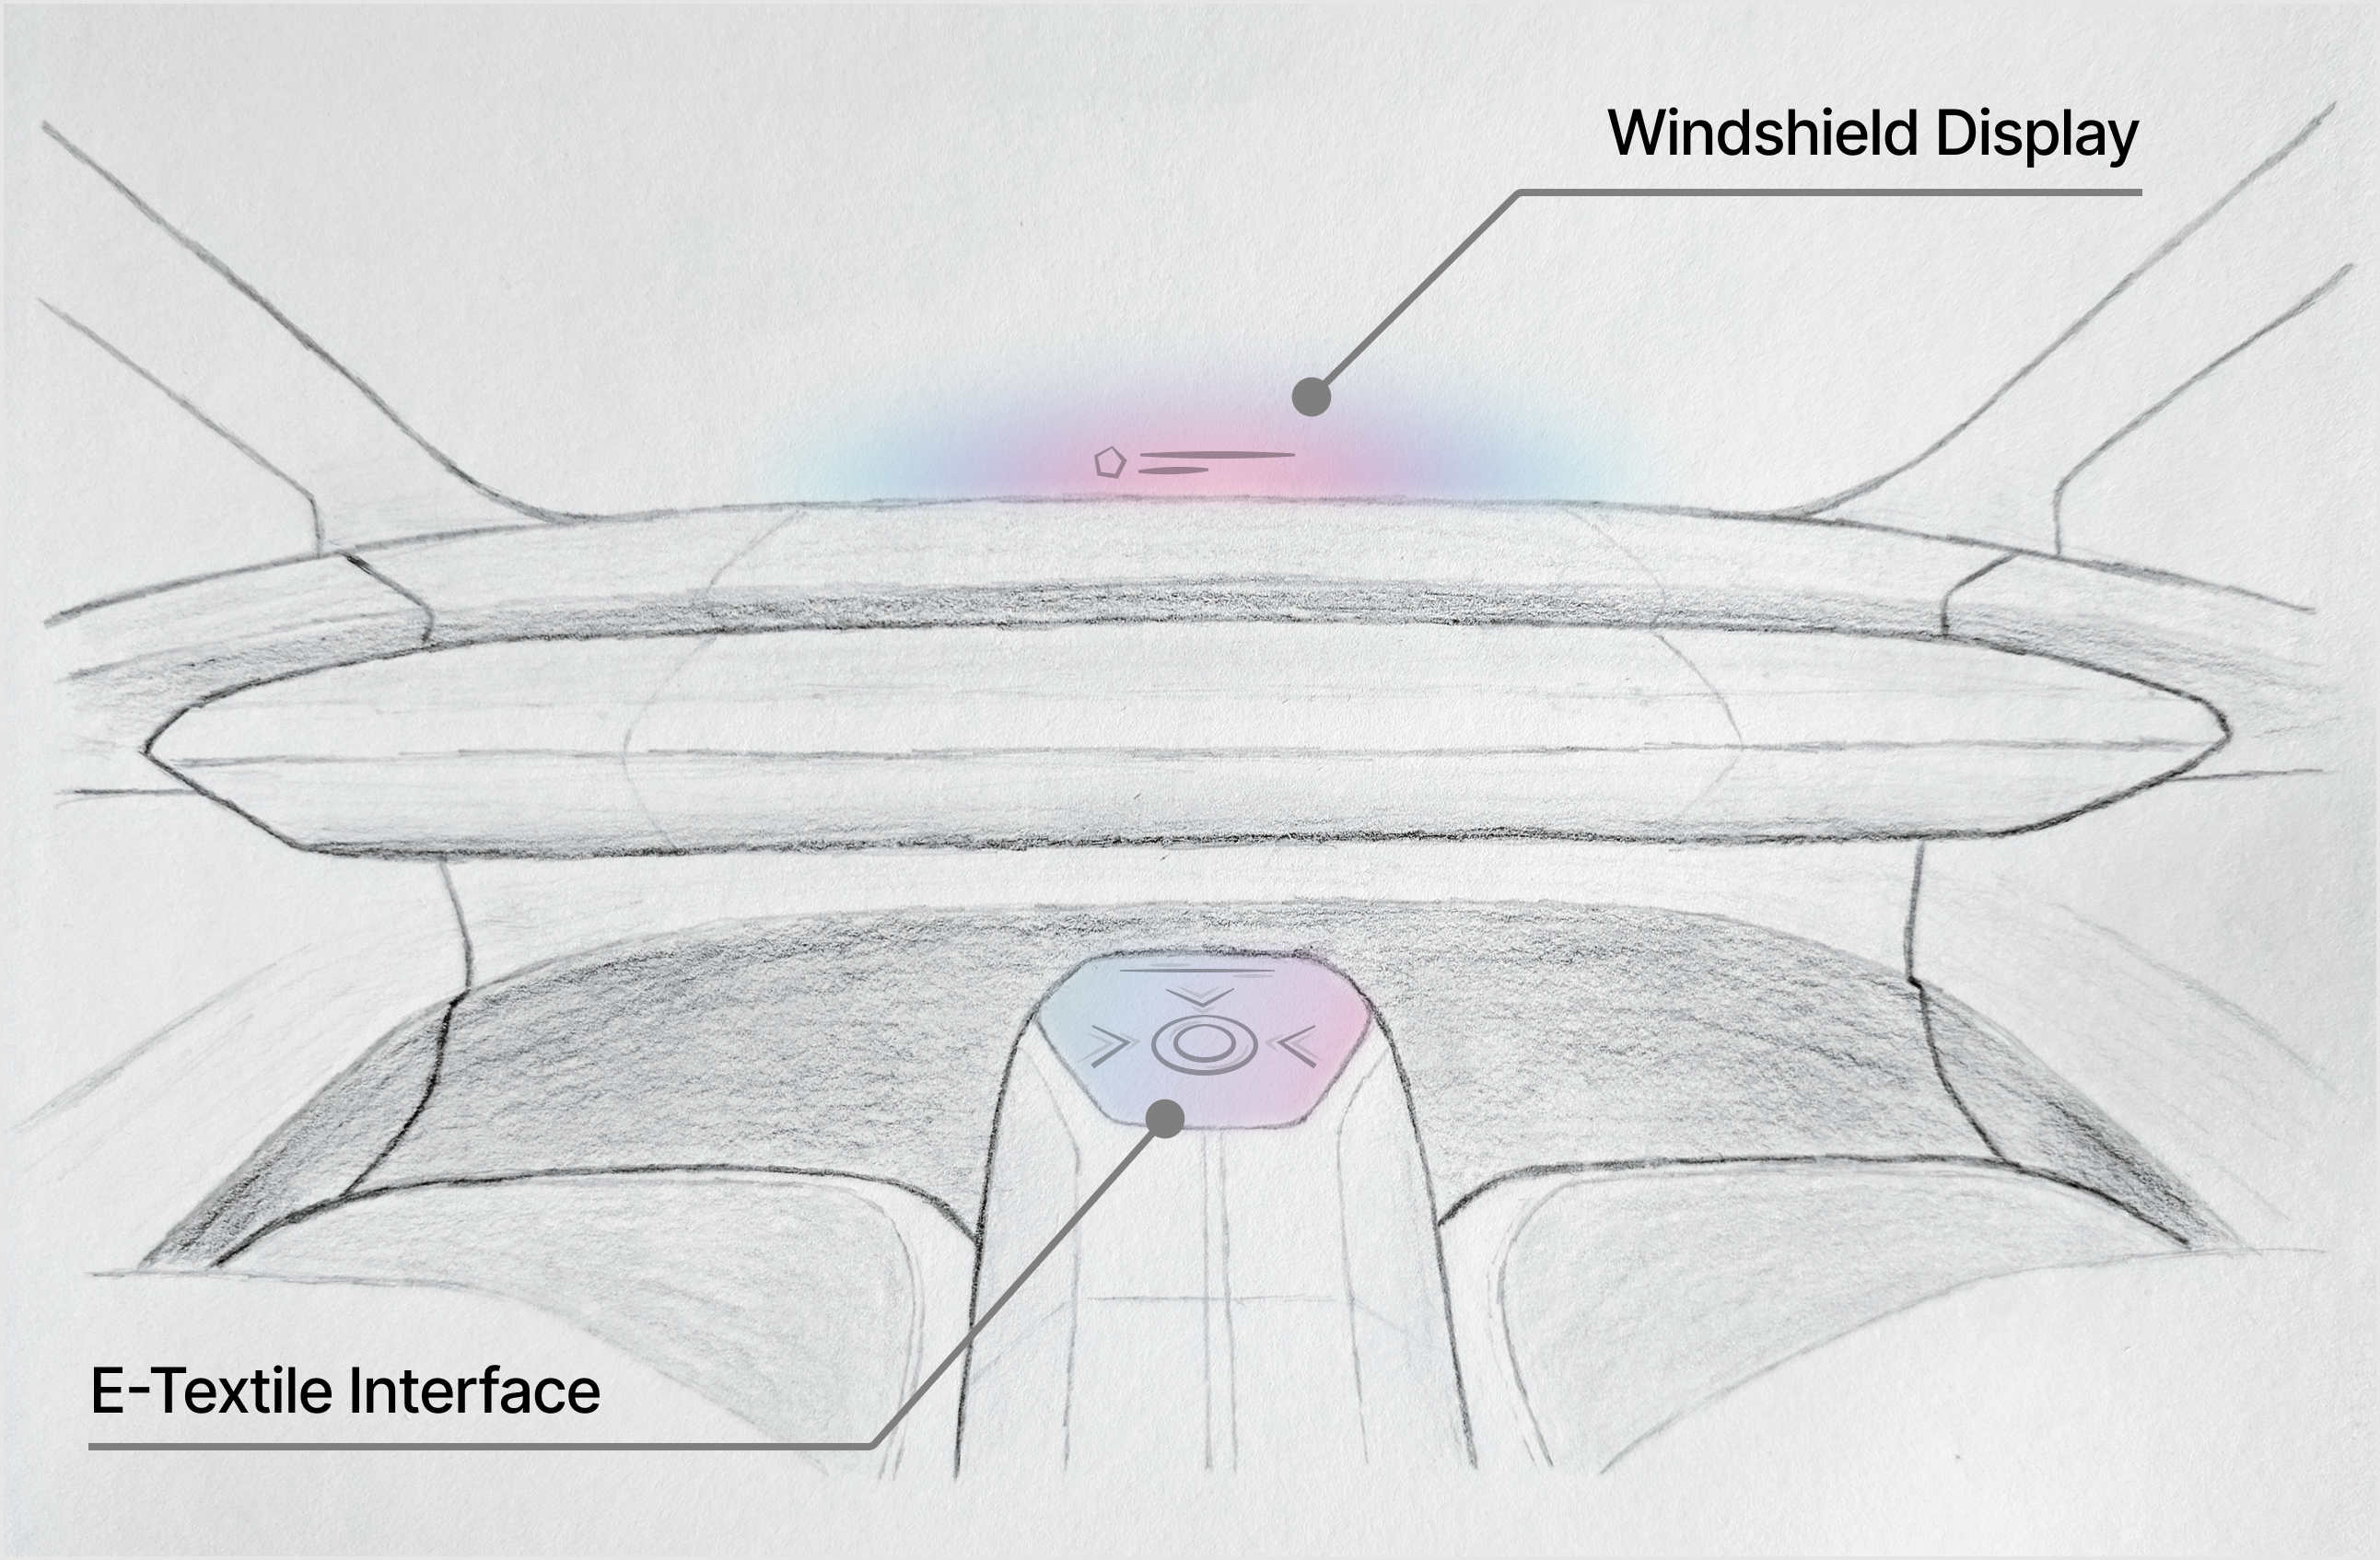
\includegraphics[width=1\linewidth]{images/Proposed Paradigm.png}
    \caption{Conceptual illustration of the proposed \gls{HMI} paradigm, combining a Windshield Display for visual output with an interactive e-textile surface for tactile input. Car interior based on the design of the BMW Neue Klasse concept \cite{bmw_neueklasse_2023}.}
    \label{fig:proposed_paradigm}
\end{figure}

The use of a \gls{WSD} as the primary visual output keeps the passenger's gaze directed forward, directly mitigating a primary cause of motion sickness \cite{diels_self-driving_2016}. As a complementary input method, an interactive e-textile surface can be integrated ergonomically on the center console armrest, while providing a natural and low visually demanding interaction with a hedonically appropriate tactile experience. Both technologies can be seamlessly and unobtrusively integrated, allowing for versatile and distraction-free \gls{NDRA}s while remaining aligned with the "living space" concept.
%By decoupling visual output from tactile input, this combined paradigm aims to create a more natural and less visually demanding interaction that addresses the key challenges of conventional interfaces.
% The use of a WSD as the primary visual output ensures that passengers can receive information without looking down and away from the direction of travel, directly mitigating a primary cause of motion sickness \cite{diels_self-driving_2016}. Furthermore when turned off it fully dispapers and alows the user to fully focus on NDRAs. Paired with this, an interactive e-textile surface for input addresses the remaining challenges. By embedding interaction into the soft, ubiquitous materials of the interior, e-textiles can be placed in ideal ergonomic locations, solving the "gorilla arm" problem \cite{berger_tactile_2019}. Unlike the "impersonal, digital, stiff, and cold objects" of today's devices \cite{brauner_interactive_2017}, the inherent warmth and rich textural properties of fabric align with the desired aesthetics of a "living space" and are better suited for "affective haptics communication" \cite{jiang_material-driven_2022}. Most importantly, the innate tactility of these interfaces provides the physical cues missing from featureless screens, creating the potential for a less visually demanding and more pleasant interaction experience.

\subsubsection{Windshield Displays}

A key component of the proposed \gls{HMI} paradigm is the use of the vehicle's windshield as the primary visual output. This concept is an evolution of the established \gls{HUD}, a technology initially developed for military aviation \cite{skirnewskaja_automotive_2022} and first introduced in cars by General Motors in 1988 \cite{weihrauch_first_1989}, that renders information in a partially-transparent display, allowing the user to comprehend it while still looking at the forward scene \cite{haeuslschmid_design_2016, skirnewskaja_automotive_2022}. The main advantage of \gls{HUD}s is that they are positioned close to the driver's natural line of sight, allowing information to be accessed quickly without the need to look down at the dashboard, thereby reducing the visual fatigue caused by switching between far and near perspectives \cite{haeuslschmid_design_2016, skirnewskaja_automotive_2022, zhu_value_2020}. While traditional \gls{HUD}s typically display limited, critical information like speed or navigation cues \cite{skirnewskaja_automotive_2022, weinberg_evaluating_2011}, the ever-increasing amount of information in modern vehicles requires new visualization concepts \cite{riegler_investigating_2018}.

One of the most promising solutions is the Windshield Display (\gls{WSD}), which Haeuslschmid et al. \cite{haeuslschmid_first_2016} describe as the "big siblings of head-up displays" that extend the display real estate to cover the entire windshield \cite{haeuslschmid_design_2016, hauslschmid_augmenting_2015}. \gls{WSD}s could be a critical component in the transition to automated vehicles by offering a multitude of benefits \cite{riegler_investigating_2018}. They can eliminate physical and visual clutter from the center console \cite{riegler_investigating_2018}, provide a single, unified interface for all in-vehicle systems \cite{gabbard_behind_2014}, and enable new gestural interaction modalities \cite{riener_gestural_2012}. The \gls{WSD}'s partial-transparency opens the door to a wide variety of Augmented Reality (\gls{AR}) applications, which could enhance in-vehicle experiences and further ease the transition from manual to \gls{HAD}  \cite{kun_arv_2017}. 

For highly automated vehicles, \gls{WSD}s have the potential to enhance user trust by increasing system transparency \cite{wintersberger_traffic_2017}.  For instance, a study by Wintersberger et al. \cite{wintersberger_traffic_2017} demonstrated that using an \gls{AR}-\gls{HUD} to create "traffic augmentation", highlighting other cars and potential hazards, significantly increased the participants' subjective feeling of trust in the automated system. Building on this, Lindemann et al. \cite{lindemann_catch_2018} demonstrated that an "explanatory windshield display", which visualizes the automation's reasoning and intended path, can significantly improve a passenger's situation awareness and understanding of the vehicle's behavior. 
 % However, the design of the information itself is crucial. Research by Dandekar et al., for instance, compared a WSD that used explicit pictograms against a more abstract, ambient light bar display around the windshield, while passengers engaged in NRDAs. They found that while both concepts successfully maintained high levels of trust and UX, the ambient light bar was actually preferred by users and provided a superior user experience, suggesting that less obtrusive, more integrated forms of information display may be more desirable than screen-based graphics, even when those screens are transparent \cite{dandekar_how_2022}.  

Beyond building trust, the \gls{WSD} can also directly influence the hedonic experience of the ride by transforming the journey itself into an engaging activity. For passengers in an \gls{AV}, a \gls{WSD} can display context-aware information, such as overlaying navigational aids onto the environment \cite{haeuslschmid_design_2016} or augmenting the view with information about points of interest \cite{haeuslschmid_first_2016}, effectively turning the act of sightseeing into an interactive learning experience \cite{matsumura_active_2018}. This directly caters to one of the possible primary \gls{NDRA}s in Avs, which is looking out the window and observing the environment \cite{ahram_what_2020, pfleging_investigating_2016}, also found to be a central factor for positive passenger experience in today's manually driven cars \cite{berger_designing_2021}. To further enhance this sense of exploration and fulfill the desires of active passengers, the \gls{WSD} could offer interactive functionalities. Passengers could, for example, zoom in on distant objects for a closer look, receive real-time translations of foreign signs, or "pause" the view to examine a fleeting scene in more detail \cite{matsumura_active_2018, pagura_window_2011}. 

The large display real estate also opens up new possibilities for entertainment and social connection. Researchers have explored concepts for in-car gaming \cite{togwell_-car_2022}, which could also invite to social interactions in the vehicle \cite{matsumura_active_2018}. This capability to support a wide range of \gls{NDRA}s is key to its potential to convert the vehicle into a true "infotainment platform" \cite{riener_automotive_2016}. Although the technology is still considered a young research field \cite{haeuslschmid_design_2016} and not yet commercially widespread due to technical, usability, and cost issues \cite{gabbard_behind_2014}, the potential can be easily evaluated in simulation \cite{riegler_investigating_2018}. Initial research has already produced several key design recommendations, addressing factors such as information placement preferences \cite{haeuslschmid_first_2016, riegler_investigating_2018}, optimal window background color and transparency \cite{riegler_adaptive_2019}, and the use of world-fixed versus screen-fixed positioning for displayed information \cite{riegler_stickywsd_2020}.

In essence, the \gls{WSD} provides a compelling solution for the visual output component of a future in vehicle \gls{HMI}. However a corresponding input modality is required to control the rich content on this new digital canvas, leading to the exploration of interactive textiles as a complementary solution.

% While the WSD provides a compelling solution for the system's visual output, the greater HMI challenge—and therefore the primary focus of this thesis—lies in the design of the tactile input modality. WSDs are an evolution of an established technology (HUDs), for which design recommendations already exist. Interactive textiles, by contrast, represent a novel paradigm for which the principles of intuitive interaction are still emerging. It is here, in the design of the physical interaction, that the core research questions of learnability, affordance, and feedforward must be addressed. Consequently, the remainder of this review will focus on establishing the state-of-the-art in designing these novel textile interfaces.


\subsubsection{Interactive E-Textiles}

While the \gls{WSD} offers a compelling solution for visual output, it requires a corresponding input modality that is ergonomic, unobtrusive, and hedonically aligned with the envisioned "living space". Interactive electronic textiles (e-textiles) present themselves as a uniquely suitable candidate to fulfill this role. 

Broadly defined, textile user interfaces are fabrics that can sense a user's physical interactions and produce responses as a result \cite{mlakar_exploring_2021}. By utilizing technologies like resistive and capacitive sensing, e.g. \cite{holleis_evaluating_2008, parzer_resi_2018, poupyrev_project_2016, goveia_da_rocha_crafting_2020, schneegass_gesturesleeve_2016, wu_project_2021, wu_zebrasense_2020}, they support a variety of versatile interaction methods that are comparable to those on conventional touch surfaces \cite{schafer_whats_2023}. The aim of research on interactive textiles is to "combine the power of digital devices with the ubiquity [and familiarity] of analog textiles" \cite[pp.~151]{brauner_interactive_2017}. By leaving the rigid shapes of today's devices behind \cite{castano_smart_2014, hamdan_sketchstitch_2018, posch_integrating_2018, poupyrev_project_2016}, e-textiles can extend the design space for \gls{HMI} and create novel input technologies that appeal to both visual and haptic perception \cite{mlakar_exploring_2021}.

%\paragraph{The Promise and Potential of E-Textiles}
\paragraph{The Potential of E-Textiles} \mbox{} \\
E-textiles offer a number of distinct advantages over conventional interfaces, particularly in addressing the pragmatic and hedonic limitations of touchscreens within the automotive context.

First, from an \textbf{aesthetic and tactile} perspective, textiles directly counter the "impersonal, stiff, and cold" materials like glass and plastic that dominate current in-vehicle interaction surfaces \cite{brauner_interactive_2017}. It is particularly attractive to overcome the boundaries between these traditionally rigid devices and soft, "human-facing materials" like fabrics \cite{olwal_e-textile_2020}.
Textiles are inherently perceived as warm, soft, and pleasant to the touch and come in a vast array of colors, forms, and structures \cite{brauner_interactive_2017}. This visual and haptic expressiveness \cite{hamdan_sketchstitch_2018} of the fabric itself is not merely decorative; combined with electronic components it provides the foundation for rich interactive experiences \cite{mlakar_design_2020} and better supports affective haptic communication \cite{jiang_gesfabri_2022}, as softer materials are consistently reported as more pleasant than stiff or coarse ones \cite{essick_psychophysical_1999}. This aligns perfectly with the goal of transforming the car into a comfortable and inviting living space \cite{schartmuller_automated_2020}.

Second, e-textiles excel in their potential for \textbf{seamless and ubiquitous integration}. This aligns with the foundational vision of ubiquitous computing, first articulated by Mark Weiser \cite{weiser_computer_1991}, which imagined computers that "weave themselves into the fabric of everyday life until they are indistinguishable from it" \cite[pp.~94]{weiser_computer_1991}. The goal is to achieve a state of "calm computing" \cite{case_calm_2015, denning_coming_1997}, where technology recedes from the foreground into our surroundings. 
%Because textiles are already omnipresent in vehicle interiors, embedding interactive functionality within them is a natural and less intrusive approach compared to artificial interfaces like touchscreens or remotes \cite{schafer_whats_2023, khorsandi_fabricar_2023}. Utilizing fabric and leather surfaces as seamless interfaces is a direct way to engage users in ubiquitous NDRAs and enrich their interaction with the environment (Khorsandi et al., 2023, p. 1439) 
Interactive textiles are a key enabler of this vision, aiming to "combine the power of digital devices with the ubiquity of analog textiles" \cite[pp.~151]{brauner_interactive_2017}. Because textiles are already a familiar, comfortable, and omnipresent material in vehicle interiors, they offer one of the most seamless, natural, and less intrusive ways of interacting with new technology \cite{brauner_interactive_2017, khorsandi_fabricar_2023, mlakar_exploring_2021, schafer_whats_2023}. With growing interest in such unobtrusive interfaces, everyday objects covered in smart textiles have the potential to become the "interfaces of the future" \cite{mlakar_design_2020}. They can thoroughly augment any object and provide "new and exciting features [...] that are difficult or impossible to realize with other solutions" \cite[pp.~1]{mlakar_design_2020}, allowing for the seamless and ubiquitous integration of controls and \gls{NDRA}s within the future car interior \cite{khorsandi_fabricar_2023}.

Third, the \textbf{physical form} of textiles offers significant ergonomic benefits. Unlike rigid electronics, textile-based devices can be shape-shifting, stretchable and bendable \cite{nanjappan_towards_2019}. This flexibility allows control interfaces to be placed in ideal ergonomic locations that are close to the passenger's body, such as on an armrest \cite{shishoo_textile_2008}, mitigating the arm fatigue associated with dashboard-mounted touchscreens \cite{berger_tactile_2019, sathyan_study_2020}. Furthermore, the material itself can be structured to provide inherent tactile guidance; for example, raised embroidery can guide a user's hand into the correct position without needing to look \cite{komor_is_2009}, a key advantage for reducing visual demand and potential motion sickness \cite{diels_self-driving_2016}. Fundamentally, these characteristics make textile interfaces an ideal medium for what Bakker and Niemantsverdriet \cite{bakker_interaction-attention_2016} call peripheral interaction. % In contrast to the focused interaction, such as demanded by touchscreens due required to visual attention, thus pulling attention away from NDRAs, a peripheral interface allows passengers to control vehicle functions without disrupting their primary task \cite{bakker_interaction-attention_2016}. 
Unlike touchscreens, which demand focused hand-eye coordination and can draw users away from their primary activity due to the required attention to interact, textile-based peripheral interfaces support unobtrusive vehicle interaction, allowing passengers to remain engaged in \gls{NDRA}s.
% In contrast to focused interaction, such as that required by touchscreens due to their high visual demand, peripheral interfaces enable passengers to control vehicle functions without diverting attention from their primary NDRA.

The importance of these hedonic qualities in driving user acceptance has been confirmed by empirical research. In a foundational study, Brauner et al. \cite{brauner_interactive_2017} evaluated user experience with an interactive motorized recliner armchair, directly comparing textile-based controls to a conventional plastic remote. Despite the remote control scoring higher on pragmatic qualities like efficiency, participants expressed a significantly higher preference and intention to use the textile interfaces. The study concluded that the primary driver for acceptance was the overall attractiveness and hedonic quality of the textile solution. Participants explicitly valued the "seamless integration of textile sensors into the design of the surrounding space" and the "cosiness of fabric", while criticizing the traditional remote as an "ugly" and "cold" element. This provides strong evidence that in a living space context, the aesthetic and material qualities of an interface can be more influential on user acceptance than its pragmatic performance.

%\paragraph{State of the Art and Application}
\paragraph{Current Applications} \mbox{} \\
The concept of interactive textiles is not new, as the field has been developing for over two decades, demonstrating its technological maturity. The modern era of e-textiles began in the late 1990s, when researchers like Post and Orth \cite{post_smart_1997} introduced techniques for embroidering interfaces with conductive thread and sensing touches through low cost capacitive circuits. 
%Since this pioneering work, a wide variety of fabrication methods have been developed, including weaving, knitting, and screen-printing conductive inks, allowing for the creation of robust and flexible touch-sensitive surfaces (Olwal et al., 2020, p. 2; Khorsandi et al., 2023, p. 1441). The technology has reached commercial viability, most notably with Google's Project Jacquard, which integrates conductive threads directly into fabrics on industrial looms (Brauner et al., 2017, p. 152).
Since this pioneering work, research has extensively explored the fabrication of various textile sensors. These methods generally fall into two categories: integrating conductive elements into standard textiles, or transforming the textile itself into a conductive fabric \cite{khorsandi_fabricar_2023}.

A wide variety of methods exist for integrating conductive threads and yarns, such as manual sewing or machine embroidery \cite{gilliland_textile_2010, hamdan_sketchstitch_2018, post_e-broidery_2000, goveia_da_rocha_crafting_2020, zeagler_textile_2012}, weaving \cite{pouta_woven_2022, wu_zebrasense_2020}, and knitting \cite{chen_design_2020, luo_knitui_2021}. Alternatively, fabrics can be made conductive through processes like coating non-conductive threads with metallic substances \cite{honnet_polysense_2020, lee_conductive_2015}, or by screen-printing conductive inks directly onto textile substrates \cite{goncalves_wearable_2018, zeagler_can_2013}. These techniques have enabled the creation of a diverse range of flexible sensors and interfaces \cite{olwal_e-textile_2020}, including touch matrices made from woven conductive thread \cite{parzer_resi_2018, parzer_flextiles_2016, poupyrev_project_2016} and multi-layer conductive fabrics \cite{leong_procover_2016, parzer_flextiles_2016, parzer_smartsleeve_2017, schneegass_gesturesleeve_2016}, thus preserving the shape-changing properties of conventional textiles. The technology has reached commercial viability, most notably with Google's Project Jacquard \cite{poupyrev_project_2016}, which incorporates conductive thread directly into fabrics on industrial looms to facilitate multitouch and gesture implementation. In fact, many recent approaches focus on creating \gls{2D} interactive surface patches \cite{leong_procover_2016, parzer_resi_2018, parzer_flextiles_2016, poupyrev_project_2016, schneegass_gesturesleeve_2016} that support gesture interfaces similar to modern multi-touch devices, enabling absolute \gls{2D} positioning, swipes, and even complex gestures like pinch-to-zoom \cite{olwal_e-textile_2020}.
%og location for consumer prutucts -> have been moved down

So far, research on e-textile interfaces has been largely dominated by two application domains: wearables \cite{heller_fabritouch_2014, jones_wearable_2020, karrer_pinstripe_2011, ono_textile_2017, parzer_smartsleeve_2017, schneegass_gesturesleeve_2016, strohmeier_zpatch_2018, yoon_timmi_2015} and smart furniture \cite{brauner_interactive_2017, heller_gardeene_2016, nabil_soft_2021, nabil_interioractive_2017, petersen_squeeze_2007}. Wearable applications leverage clothing to interact with devices \cite{nowak_shaping_2022}, with examples ranging from touchpads on trousers \cite{heller_fabritouch_2014} to gesture-sensing sleeves \cite{parzer_smartsleeve_2017}. In parallel, researchers have explored augmenting domestic environments by integrating controls into furniture, such as an armchair with embedded textile controls \cite{brauner_interactive_2017} or motorized curtains that can be opened and closed through touch gestures \cite{heller_gardeene_2016}.

However, despite the proven technical feasibility and potential applications, the transition to the consumer market has been challenging. Only a handful of products were developed using Google's Jacquard technology, such as the Levi's Commuter, Trucker, and Sherpa Jackets \cite{poupyrev_more_2017, poupyrev_smarter_2019}, as well as the Saint Laurent Cit-E \cite{poupyrev_smarter_2019} and Samsonite Konnect-I \cite{poupyrev_make_2020} backpacks. Furthermore, as of April 2023, Google discontinued the required Jacquard mobile app, rendering the core functionality of these products unusable \cite{bradshaw_google_2023}. This leaves a notable void in the market; to the best of our knowledge, there are currently no true consumer products featuring fabric with integrated touch-sensing capabilities, if one excludes smart home devices, like the Google Nest Mini \cite{google_store_google_nodate}, which often utilize conventional capacitive touch sensors placed underneath a passive fabric layer.


%\paragraph{Current Research Landscape for e-textiles for in-vehicle interaction}
\paragraph{Current Research Landscape on In-Vehicle E-Textiles} \mbox{} \\
Despite the opportunities presented by fabric-rich car interiors, there has been limited work at the intersection of e-textiles and \gls{HVI} \cite{khorsandi_fabricar_2023}. The existing research in this area can be broadly categorized. One line of work involves wearable physiological sensors integrated into jackets \cite{van_langenhove_smart_2004}, bracelets \cite{caon_wearable_2014}, or seat-belts \cite{wagner_16_2013} to detect the driver's biometrics, such as heart rate, breathing level, or concentration, with the vehicle adapting to passengers accordingly. Another area focuses on wearable devices for in-vehicle interaction, such as the fabric-based wrist-worn device by Nanjappan et al. \cite{nanjappan_towards_2019} controlling media and navigation through wrist and touch gestures. 
%While such wearable solutions offer intriguing possibilities for personalized control, this work intentionally focuses on non-wearable interfaces for several reasons. Requiring specialized clothing to interact with a car could be perceived as obtrusive by passengers and might present a barrier to adoption. It limits the interaction to only those wearing the specific garment, contrasting with the goal of creating a "walk-up-and-use" experience that is inherently shareable among all occupants of the vehicle.

Research on non-wearable textile surfaces, in line with our envisioned \gls{HMI} paradigm, is even more scarce. To the best of our knowledge, it is primarily limited to industry concepts like BMW's "Shy Tech" \cite{bmw_group_bmw_nodate}, academic posters \cite{khorsandi_functioning_2022}, and demonstrations \cite{dong_disappearing_2019} which often lack reported results from formal user studies. A notable exception is the work by Khorsandi et al. \cite{khorsandi_fabricar_2023} on FabriCar, which integrated textile sensors into a steering wheel, headrest, and seat-belt to study media control interactions. Their study made a significant contribution by demonstrating that textile interactions led to substantially less eye distraction compared to screen-based interactions during driving tasks.
% Old Ending:
% While this work validates the pragmatic potential of textile interfaces for reducing driver distraction, it leaves open the question of how to design such interfaces for the future context of autonomous vehicles, where the primary challenges shift from minimizing driver distraction to ensuring a hedonically rich and engaging user experience.

\paragraph{Summary} \mbox{} \\
While this work validates the technical feasibility and the pragmatic potential of textile interfaces, the primary challenges for the passenger-focused \gls{AV} context remain unaddressed. It is not yet clear how to design these novel surfaces to be immediately understood and effectively used by novice passengers, ensuring an experience that is not only hedonically rich but also fundamentally intuitive. Therefore, a deeper investigation into the principles of learnability and interaction guidance is required. 

% The ability to embed sensors ubiquitously into existing textile objects provides the advantage of creating simple control interfaces that are "less intrusive than other approaches" (Brauner et al., 2017, p. 152). This aligns with a design philosophy that moves toward minimalistic, aesthetically-integrated form factors that enrich our interaction with the existing environment (Khorsandi et al., 2023, p. 1439) [65, 79, 85]. When paired with a WSD that eliminates the visual clutter of a traditional dashboard, the e-textile input surface completes a holistic HMI that is both highly functional and unobtrusive. The result is an interface that supports the vision of "Interactive Interiors" (Nabil et al., 2017, p. 379) and moves the vehicle closer to the calm, integrated, and intuitive environment that the "living space" concept demands.


\subsection{Research Gap: Intuitive Interaction}

% Having established interactive textiles as a promising solution to the limitations of conventional in-vehicle interfaces, the central challenge now shifts from technological feasibility to interaction design. The very novelty of e-textiles is their primary hurdle: because most users have no established mental models for interacting with them, there is significant potential for confusion regarding where and how to perform an interaction. This presents a critical usability problem, as the HMI community shares the belief that such interfaces must not rely on training or explicit instructions to be used effectively.

Having established interactive textiles as a promising solution to the limitations of conventional in-vehicle interfaces, the central challenge now shifts from technological feasibility to interaction design. The very novelty of e-textiles is their primary hurdle: because most users have likely never encountered interactive textiles due to the lack of existing consumer products, they are not yet familiar with them \cite{mlakar_exploring_2021} and have yet to establish mental models for interacting with them, potentially leading to confusion regarding where and how to perform an interaction \cite{dong_disappearing_2019, mlakar_exploring_2021}. This presents a critical usability problem, as there is a shared belief in the \gls{HMI} community that "such interfaces must not rely on users getting training or explicit instructions or manuals to successfully interact with them" \cite[pp.~1159]{mlakar_exploring_2021}. To create such an onboarding-free "walk-up-and-use" experience, the interface itself must passively inform or remind the user about possible interactions \cite{mlakar_exploring_2021}. 
% This requires a deep understanding of how an interface can guide a user before they act.

The practical importance of this challenge is perfectly illustrated by comparing two early commercial products that used the same Google Jacquard \cite{poupyrev_project_2016} technology. The first product, the Levi's Commuter Jacket \cite{poupyrev_more_2017}, embedded an interactive area in the sleeve cuff (see Fig. \ref{fig:Levi's Commuter Jacket}). However, as Mlakar et al. \cite[pp.~1159]{mlakar_exploring_2021} critique, the jacket "does not [...] offer clear differentiation between the interactive and non-interactive area [...] nor does it give any indication of what actions are possible on that surface". This creates a situation where the possibility for interaction is effectively hidden, forcing a user to rely on a manual to know \textit{where} and \textit{how} to interact \cite{mlakar_exploring_2021}. In contrast, the Samsonite Konnect-I Backpack \cite{poupyrev_make_2020} used the same technology but with much more effective design. Its interactive strap clearly marks the interactive area through color and texture (see Fig. \ref{fig:Samsonite Konnect-I Backpack}). Its ribbed surface clearly suggests a sliding gesture, while its width hints that the interaction could be performed with a whole palm, instead of a single finger, providing an intuitive, built-in clue about how to interact \cite{mlakar_exploring_2021}. This comparison demonstrates that without deliberate design cues that make interaction possibilities obvious, even a technologically capable interface can fail in usability.

\begin{figure}
     \centering
     \begin{subfigure}[b]{0.49\textwidth}
         \centering
         \includegraphics[width=\textwidth]{images/Google Jacquard/Levi's Commuter Trucker Jacket.png}
         \caption{Levi's Commuter Jacket \cite{poupyrev_more_2017}}
         \label{fig:Levi's Commuter Jacket}
     \end{subfigure}
     \hfill
     \begin{subfigure}[b]{0.49\textwidth}
         \centering
         \includegraphics[width=\textwidth]{images/Google Jacquard/Samsonite Konnect-I Backpack.png}
         \caption{Samsonite Konnect-I Backpack \cite{poupyrev_make_2020}}
         \label{fig:Samsonite Konnect-I Backpack}
     \end{subfigure}
        \caption{Different implementation strategies of Google's Jacquard Technology \cite{poupyrev_project_2016} in consumer products.}
        \label{fig:Google's Jacquard Technology}
\end{figure}

% This comparison demonstrates that without the deliberate design of signifiers to create perceptible affordances, even a technologically capable interface can fail in usability.

%\subsubsection{The Learnability Problem: The Need for Intuitive Interaction}
\subsubsection{Learnability and the Need for Intuitive Interaction}

The ultimate goal for any novel interface is to achieve intuitive interaction. An intuitive interface is one that feels "easy" or "natural" to use, allowing a person to successfully operate it without undergoing a lengthy or effortful learning process \cite{mignonneau_designing_2005}. This sense of ease arises because the interaction effectively leverages a user's existing knowledge \cite{blackler_investigating_2010, khan_intuitive_2017}, both subconscious knowledge of physical affordances (e.g., buttons are for pressing) and conscious knowledge from past experiences or cultural conventions \cite{blackler_towards_2015}. In essence, intuitive interaction occurs when a user can immediately and non-consciously use an interface by drawing upon this stored knowledge \cite{chen_affordance_2017}.

This distinction is captured perfectly by Donald Norman's foundational concept of \textit{knowledge in the head} versus \textit{knowledge in the world} \cite{norman_design_2013}. "Knowledge in the head" is what we possess internally in our memory, such as learned skills and cultural conventions. "Knowledge in the world" refers to the information that is readily available and perceivable in our environment, such as visual signifiers, physical constraints, and natural mappings. While it is best when a user has considerable "knowledge in the head", a designer can place sufficient cues into the product itself, so that good performance is possible even without prior experience.

As Schäfer et al. \cite{schafer_whats_2023} note, the literature on textile interfaces is dominated by examples that require "knowledge in the head", forcing users to learn how a product works before use. Because most users have no prior experience with interactive textiles, they lack the stored "knowledge in the head" needed to interact intuitively. This creates a learnability gap, where the novelty of the interface prevents the natural, non-conscious interaction that users have come to expect from mature technologies. 
However, this challenge also presents a unique opportunity. Naumann et al. \cite{naumann_intuitive_2007} argue that aesthetics is the very gateway to intuitive use; it is the visual and tactile appeal of an object that invites a user to touch and explore, allowing them to then apply their prior knowledge. For novel interfaces, aesthetics can be "the key to the technology that lies behind" \cite[pp.~135]{naumann_intuitive_2007}.
Therefore, the central design problem is how to leverage the inherent aesthetic qualities of textiles and combine them with sufficient "knowledge in the world", guiding users toward correct interactions in a way that feels both intuitive and engaging \cite{schafer_whats_2023}.
% The central design problem, therefore, is how to bridge this gap by embedding sufficient "knowledge in the world" into the interface itself, guiding users toward correct interactions in a way that still feels intuitive.

% Herein lies the fundamental challenge for e-textiles: the very mechanism that enables intuitive use, which is a user's previous experiential knowledge, is precisely what is missing. As established, most users have no prior experience with interactive textiles and therefore lack the stored knowledge needed to interact intuitively. This creates a "learnability gap", where the novelty of the interface prevents the natural, non-conscious interaction that users have come to expect from mature technologies. The central design problem, therefore, is how to bridge this gap. If the interface cannot rely on a user's past, it must effectively teach them in the present, guiding them toward correct interactions in a way that still feels intuitive.

%\subsubsection{Feedforward as the Guiding Framework}
\subsubsection{Feedforward as a Guiding Framework}

% OG Feedforward Intro
\begin{comment}
    
% To understand how an interface can guide a user, it is helpful to analyze the interaction process itself. Any interaction between a person and a product can be seen as a continuous exchange of information. 
The primary way a designer can embed this "knowledge in the world" into an interface is by carefully considering the information exchanged between the product and the user.
This exchange can be broken down into what happens before, during, and after the user’s action \cite{vermeulen_crossing_2013}. The information the product provides during or after the user acts is commonly known as \textbf{feedback} \cite{wensveen_interaction_2004}. Wensveen et al. \cite{wensveen_interaction_2004} cite the dictionary definition of feedback  as "the return of information about the result of a process or activity" \cite{harpercollins_publishers_american_nodate}. For example, when a user pushes a power button to turn on a monitor, they receive feedback during the action: they feel the travel of the button and a "click" once it is fully depressed. After the action is complete, they receive further feedback when the screen lights up, confirming the result of their action.

However, a crucial part of the interaction happens before any action is taken. Before the user ever touched the button, the product had already offered information that communicated how it could be used. This information that is available before an action takes place is called \textbf{feedforward} \cite{wensveen_interaction_2004}. In the power button example, the fact that the button was protruding from its housing and was roughly the size of a fingertip served as feedforward, suggesting to the user that it could be pushed. While feedback confirms an action that has already occurred, feedforward makes the action discoverable in the first place.

To solve the learnability problem for novel interfaces with which users have no prior experience, thus no "knowledge in the head", the focus must therefore shift to this critical pre-interaction phase. While feedback is essential for a good user experience, it is the effective design of feedforward that makes a new system intuitively usable without any onboarding.
\end{comment}

The primary way a designer can embed this "knowledge in the world" into an interface is by carefully considering the information exchanged between the product and the user.
This exchange can be broken down into what happens before, during, and after the user’s action \cite{vermeulen_crossing_2013}. The information the product provides during or after the user acts is commonly known as \textbf{feedback} \cite{wensveen_interaction_2004}. Wensveen et al. \cite{wensveen_interaction_2004} cite the dictionary definition of feedback as "the return of information about the result of a process or activity" \cite{harpercollins_publishers_american_nodate}. For example, when a user pushes a power button to turn on a monitor, they receive feedback during the action: they feel the travel of the button and a "click" once it is fully depressed. After the action is complete, they receive further feedback when the screen lights up, confirming the result of their action.

However, a crucial part of the interaction happens before any action is taken. Before the user ever touched the button, the product had already offered information that communicated how it could be used \cite{wensveen_interaction_2004}. This pre-interaction guidance is provided by two related, but distinct, concepts: affordance and feedforward. 

The concept of affordance was coined by Gibson \cite{gibson_theory_1977}, and is described as all of the action possibilities that are present in the environment, independent of an individual's ability to recognize them. 
% In the context of HCI, Donald Norman \cite{norman_design_2013} adapted this concept to focus on perceived affordances: the aspects of a design that suggest to a user how the object should be used. Norman later argued that the term signifier is more accurate for these perceptible cues \cite{norman_way_2008}. The core function of a perceived affordance, or signifier, is to suggest how a user can physically interact with an object. For example a handle affords pulling, a button affords pushing, and a knob affords turning.
For design, the focus shifts to perceptible affordances, those possibilities for interaction that a user can correctly identify based on an object's design \cite{mlakar_exploring_2021}. William Gaver \cite{gaver_technology_1991} further refines this by categorizing affordances based on the alignment between perception and reality. Gaver referes to \textbf{perceptible affordances} as interaction possibilities that were correctly identified by users based on an object’s design. \textbf{Hidden affordances} are actual possibilities that are not perceived by the user, which can decrease usability, as was the case with the previously discussed Levi's Commuter Jacket \cite{poupyrev_more_2017} interactive sleeve. Conversely, \textbf{false affordances} are perceived possibilities that do not actually exist, leading to user error. As emphasized by Mlakar et al. \cite{mlakar_exploring_2021}, it is important to note that, following Gaver's definitions, an affordance only informs us about the possibilities for interaction (e.g., that a slider can be moved), not necessarily the function or result of that interaction (e.g., that moving the slider controls volume). The core function of an affordance is to suggest \textbf{\textit{how}} a user can physically interact with an object. For example a handle affords pulling, a button affords pushing, and a knob affords turning.

While affordances suggest possible actions, \textbf{feedforward} serves the distinct purpose of informing the user about \textbf{\textit{what will happen}} as a result of that action. As clarified by Vermeulen et al. \cite{vermeulen_crossing_2013}, this distinction is essential: an affordance reveals the \textit{physical action} and answers the question, "What can I do?", while feedforward reveals the \textit{functional result} by answering the question, "What will happen if I do it?". 

The power button example perfectly illustrates this synergy:
% \begin{figure} [h!]
%     \centering
%     \includegraphics[width=0.5\linewidth]{images/PXL_20250711_080025061.jpg}
%     \caption{Enter Caption}
%     \label{fig:enter-label}
% \end{figure}
\begin{itemize}
    \item Affordance: The button's protruding shape and size affords the physical action of pushing with a finger.
    \item Feedforward: A universal power symbol printed on it communicates that the result of pushing will turn on the device.
    \item Feedback: The tactile click and the screen lighting up confirm the action was successful.
\end{itemize}

This framework allows us to differentiate between the types of pre-action cues. Building on the foundational definitions by Wensveen et al. \cite{wensveen_interaction_2004}, which were later expanded by Vermeulen et al. \cite{vermeulen_crossing_2013} based on Hartson's expanded definition of affordance types \cite{hartson_cognitive_2003}, we categorize these cues as follows:

%Adapted from the foundational definitions by Wensveen et al. \cite{wensveen_interaction_2004} and the clarification by  Vermeulen et al. \cite{vermeulen_crossing_2013} based on Hartson`s \cite{hartson_cognitive_2003} expanded definition of affordance types, we categorize these cues as follows: 

\textbf{Inherent Feedforward Cues} are directly derived from the physical properties of an object and appeal to our perceptual-motor skills, such as the button's position, size and shape \cite{wensveen_interaction_2004}. This concept is closely aligned with the idea of physical affordance \cite{hartson_cognitive_2003}, as it communicates the information of possible interactions and how they can be carried out \cite{vermeulen_crossing_2013, wensveen_interaction_2004}. 

\textbf{Augmented Feedforward Cues}, by contrast, is information that comes from an additional source and appeals to a user's cognitive skills \cite{wensveen_interaction_2004}.
%(cognitive affordance)
% These cues are not built into the physical form in the same way as inherent feedforward cues, but they added on top to provide further guidance, revealing the function of an action. This can take the form of words, pictograms, or other signals like lights and sounds. A text label reading "Press to power on/off" next to the button or a pulsing light on the button symbolizing a chance to change the products power state are both examples of augmented feedforward.
These cues are not built into the physical form in the same way as inherent feedforward cues, but they are added on top to provide further guidance \cite{vermeulen_crossing_2013, wensveen_interaction_2004}. While these cues are often used to reveal the function of an action, e.g., a power symbol on a button \cite{vermeulen_crossing_2013}, we argue that they can also serve the critical purpose of clarifying an ambiguous or hidden physical affordance \cite{gaver_technology_1991, hartson_cognitive_2003}. This can take the form of words, pictograms, symbols or other signals like lights and sounds \cite{wensveen_interaction_2004}. For instance, a text label reading "Press to power on/off" next to the button or a pulsing light on the button are both examples of such augmented feedforward cues.

While Wensveen et al. \cite{wensveen_interaction_2004} and Vermeulen et al. \cite{vermeulen_crossing_2013} also describe a third category, functional feedforward, which informs the user about the general purpose of a product, the distinction between inherent and augmented feedforward is the most critical for analyzing the design of specific interface cues. This distinction provides the necessary framework to systematically investigate how different methods of embedding "knowledge in the world" can guide a first-time user.

% This aligns with the work of O'Brien et al., who argue that such feedforward techniques are essential for creating an intuitive interaction, as they guide the user’s "guessing process" by managing their expectations within a lenient learning environment where exploration is encouraged. 

% Ultimately, the effective use of these feedforward techniques is what enables intuitive interaction. O'Brien et al. support this view, defining intuitive HCI as interactions within "lenient learning environments" that allow a user to combine prior experience with feedforward methods to achieve their goals. They argue that designers can guide the user’s "guessing process" by using feedforward to manage their expectations about a system's response, making the interaction feel discoverable and predictable even for a novice user.

% This approach is central to enabling intuitive interaction, which O’Brien et al. define as a process where users effectively apply feedforward methods in a "lenient learning environment" to achieve their goals.

%\subsubsection{A Framework for Feedforward: The Feedforward Matrix}
\subsubsection{The Feedforward Matrix} \label{sec:feedforward-matrix}

While the distinction between inherent physical feedforward and augmented functional feedforward is useful, many cues in the real world are not so clearly defined. A cue can be partially integrated into an object's form, or it can simultaneously hint at both the action and the function. To systematically investigate how different cues guide a first-time user, a more nuanced framework is needed. Therefore, we propose a \textbf{Feedforward Matrix} (see Fig. \ref{fig:feedforward-matrix-empty}): a two-dimensional space that categorizes pre-interaction cues along two continuous axes.

\begin{figure} [h!]
    \centering
    \includegraphics[width=1\linewidth]{images/Feedforward Matrix/Feedforward Matrix Empty V2.png}
    \caption{The Feedforward Matrix, a two-dimensional framework for classifying pre-interaction cues based on their Integration Level and Information Type.}
    \label{fig:feedforward-matrix-empty}
\end{figure}

The first axis represents the \textbf{Integration Level}, describing how a cue is delivered in relation to the physical object. This is a spectrum ranging from Embedded/Inherent (where the cue is the physical form, such as its shape or texture) to Augmented/External (where the cue is an additional layer of information, such as a separate text label on a screen). An integrated LED light within a translucent button, for example, would fall somewhere in the middle of this spectrum; it is an augmented component, but it is physically part of the object's surface, making it feel more embedded than a separate instruction.

The second axis represents the \textbf{Information Type}, describing what kind of information the cue communicates. This is a spectrum based on the distinction clarified by Vermeulen et al. \cite{vermeulen_crossing_2013}. At one end is Affordance-Clarifying (action-focused), where cues answer the question, "What can I do and how?". At the other end is Function-Revealing (result-focused), where cues answer the question, "What will happen if I do it?". A cue can exist anywhere along this spectrum. For instance, the pulsing pattern of a light primarily clarifies an affordance ("interact here!"), but the presence of light itself carries a cultural association with electrical power, thus subtly revealing a potential function.

%\subsubsection{State of the Art in E-Textile Affordances and Cues / Emerging Design Principles for Tactile and Textile Interfaces}
\subsubsection{Feedforward and Affordances in E-Textiles}

Despite the technical maturity of e-textiles, many researchers \cite{jiang_gesfabri_2022, mlakar_exploring_2021, nowak_shaping_2022, schafer_whats_2023} note that the design of their interactive elements has received comparatively little attention. Much of the \gls{HMI} research in this area, as described by Schäfer et al. \cite[pp.~3]{schafer_whats_2023}, has focused on "questions of technical implementation and feasibility demonstrations". Mlakar et al. \cite[pp.~1160]{mlakar_exploring_2021} suggest this is a natural consequence of the field's early stage, where "technological innovation and fabrication are the main focus, and that the design of interactive elements is rarely a primary consideration when creating innovative prototypes". As a result, affordances or feedforward cues play a minor role in the current body of work on smart textile user interfaces \cite{mlakar_exploring_2021}, resulting in a lack of guidelines and recommendations regarding their design \cite{schafer_whats_2023}.

% This technology-driven focus has often led to a "bottom-up" design approach, where researchers first create a function and then find a matching gesture for it \cite{jiang_gesfabri_2022}. According to Jiang et al. \cite{jiang_gesfabri_2022}, the consequence of this approach is that the "relationship between the types of gestures and the affordance of the surfaces of e-textile received limited attention". This can result in interfaces that are not inherently intuitive and, as Mlakar et al. \cite{mlakar_exploring_2021} point out, often "require instructions to be understood", as the perceivable "knowledge in the world" is not available.

This technology-driven focus has often led to a "bottom-up" design approach, where researchers first create a function and then find a matching gesture for it \cite{jiang_gesfabri_2022}. Examples of such systems include RESi \cite{parzer_resi_2018}, which uses resistive yarn for tap and swipe gestures, FabricKeyboard \cite{wicaksono_fabrickeyboard_2017}, a deformable textile surface, and other interfaces designed for specific interactions like squeezing, e.g., Skweezee System \cite{vanderloock_skweezee_2013}, pinching, e.g., Pinstripe \cite{karrer_pinstripe_2011}, or grabbing folds of fabric, e.g., Grabrics \cite{hamdan_grabrics_2016}. According to Jiang et al. \cite{jiang_gesfabri_2022}, the consequence of this approach is that the "relationship between the types of gestures and the affordance of the surfaces of e-textile received limited attention". This can result in interfaces that are not inherently intuitive. For example, despite the high gesture recognition rate of the Skweezee System \cite{vanderloock_skweezee_2013}, participants found it difficult to form meaningful gestures on their own that were easy to remember and reproduce \cite{jiang_gesfabri_2022}. Similarly, the pre-defined behavior of Pinstripe \cite{karrer_pinstripe_2011} did not align with user expectations, particularly for a 'move forward' command in a menu \cite{jiang_gesfabri_2022}. As a result, such interfaces often require instructions to be understood \cite{mlakar_exploring_2021}, as the perceivable "knowledge in the world" is not available.

% However, a body of work is now emerging that shifts the focus toward deliberately designing well-understood physical affordances to support high usability and intuitive interaction \cite{jiang_gesfabri_2022}. This research has begun to produce initial design explorations with helpful insights \cite{mlakar_signifiers_2025, mlakar_exploring_2021, dong_disappearing_2019} as well as guidelines and recommendations based on user testing \cite{nowak_investigating_2025, schafer_whats_2023, nowak_shaping_2022, jiang_gesfabri_2022, mlakar_design_2020, brauner_interactive_2017} for textile interfaces.

However, a body of work is now emerging that shifts the focus from purely technical explorations toward deliberately designing user-centered textile interfaces. This research follows two complementary paths. One path focuses on establishing foundational guidelines for \textbf{haptic perception} \cite{mlakar_design_2020, nowak_shaping_2022, nowak_investigating_2025, schafer_whats_2023}, evaluating the recognizability of different shapes, profiles, and textures to support clear tactile guidance and eyes-free use. 
While these findings are critical for the practical construction of any tactile interface, the other stream of research focuses on how to leverage these physical properties to create \textbf{intuitive interactions}.  This research has begun to produce initial design explorations with helpful insights \cite{dong_disappearing_2019, mlakar_exploring_2021, mlakar_signifiers_2025} as well as guidelines and recommendations based on user testing \cite{jiang_gesfabri_2022, mlakar_design_2020} for textile interfaces.


\paragraph{Foundational Design Explorations} \mbox{} \\
A key example of this emerging focus on affordances is the design exploration presented in a pictorial by Mlakar et al. \cite{mlakar_exploring_2021}. The authors' stated goal was to move beyond a technology-driven approach and to systematically explore the design space of textile interfaces from a human-centered perspective. They sought to understand the "intricate relationship between the physical design of textile user interfaces [...] and how this changes users' perception of which gestures the interface supports" \cite[pp.~1160]{mlakar_exploring_2021}. To do this, an interdisciplinary team created and reflected upon a large collection of textile samples, exploring how different visual (shape, color) and haptic (texture, details) properties could communicate possibilities for interaction.

Their main contribution is a set of five clusters of findings and insights derived from this process. These insights highlight how specific design choices influence an interface's perceived affordances. For instance, they discuss how \textbf{ergonomics}, such as the size of an element or the shape of the surface beneath it, can suggest whether to interact with a single finger or a whole hand. They note that \textbf{visual affordances} are critical, as they provide the first hints for interaction, with color helping to create focus while shape is more important for communicating the required gesture. Furthermore, they explore the \textbf{perception of textures} and the innate \textbf{direction of movement} in fabrics, noting that some materials can afford sliding in one direction while resisting it in another, much like stroking a cat's fur. Finally, they advocate for an \textbf{economic usage of design elements}, warning that overloading an interface with complex haptics can lead to "haptic chaos" if not fabricated perfectly.

Crucially, Mlakar et al. \cite[pp.~1165]{mlakar_exploring_2021} present these findings as qualitative insights from their annotated portfolio and explicitly state that they "could not conduct a user study to formally evaluate [their] assumptions". This work therefore provides a rich vocabulary and a set of exploratory concepts for designing textile affordances, laying the groundwork for the more empirical, user-tested investigations that were to follow.

Building directly on this exploratory work, Mlakar et al. \cite{mlakar_signifiers_2025} would later shift their focus from surface gestures to more complex, "textile-specific interactions" such as pulling, twisting, folding, and knotting. 
This approach follows the strategy of "material-specific e-textile interaction design" proposed by Gowrishankar et al. \cite{gowrishankar_strategy_2017}, who argued that designers should derive interactions from the inherent physical properties and deformable qualities of the fabric itself, rather than simply replicating digital controls on a textile surface.
Using a Research through Design approach, they conducted a workshop where designers created 50 samples embodying these types of interactions, with a specific focus on identifying the \textbf{signifiers} used to communicate them to the user. The term "signifier" was proposed by Norman \cite{norman_way_2008} to describe intentionally placed cues that offer guidance on how to interact with the world, in contrast to affordances, which are the inherent action possibilities of a material or object.
The primary contribution of this work is the identification of three distinct categories of signifiers relevant to textile interface design. The first two, \textbf{Visual Signifiers} (e.g., color, shapes, graphics) and \textbf{Textile Signifiers} (e.g., textile contrasts, attributes and textures), confirm previously discussed design elements by research \cite{barati_affordances_2019, jiang_gesfabri_2022, mlakar_exploring_2021, mlakar_design_2020, nowak_shaping_2022, schafer_whats_2023}. However, the authors introduce a novel and important third category: \textbf{Staging Signifiers}. This category refers to how the interface is supported by its surrounding environment, such as the structure underneath it, its position and orientation in space, or the inclusion of non-textile materials that guide the interaction. For instance, providing the first step of an interaction (like a single tissue pulled from a box) or a protruding element underneath a textile surface suggesting to push it down are both powerful staging signifiers.

Beyond identifying these categories, the authors discuss observations from a user exploration session which revealed several key design considerations. They emphasize the \textbf{importance of visual perception}, noting that even for tactile interfaces, users tend to try and understand an interface visually before touching it. They also advocate for an \textbf{economic use of signifiers}, warning that using too many cues from different categories can lead to redundancy and unnecessary complexity. Perhaps most interestingly, they observed that signifiers that were familiar from other digital interfaces (e.g., arrows indicating direction) were more effective at communicating an interaction than associations with non-interactive everyday objects (e.g., an interface resembling a tissue box did not effectively communicate a "pulling" action). This suggests that even "natural" textile interactions may require clear, learned signifiers rather than relying solely on real-world metaphors. This work provides a rich, categorized vocabulary for intentionally designing cues for complex textile interactions.

% Another foundational exploration that specifically investigates feedforward for "disappearing" textile interfaces was conducted by Dong \cite{dong_disappearing_2019} in an automotive context. 
Bridging the gap between pure exploration and formal evaluation, the work by Dong \cite{dong_disappearing_2019} presents an early investigation of different inherent feedforward modalities for a "disappearing" textile interface in an automotive context. 
The work aimed to address the confusion users face when an interface is seamlessly embedded into a soft surface, such as a vehicle seat. The research designed and tested four different feedforward modalities for a simple volume adjustment task: a baseline with no feedforward, two visual cues (a static and a dynamic light pattern), and a physical, shape-changing cue. 

In a user test with 25 participants, Dong \cite{dong_disappearing_2019} found that the \textbf{shape-changing feedforward} was particularly expressive and effective at "triggering the users to interact with it". The physical nature of the shape-changing cue was noted to be easier to find and use via haptic perception, thereby reducing visual attention demand. The study's key finding was that a \textbf{combination of the shape-changing cue and the dynamic light pattern} presented the highest perceived affordance and resulted in the best user experience. 
% This early work is significant as it was one of the first to systematically compare different inherent feedforward modalities on a textile HMI, demonstrating a promising approach for designing more intuitive and enjoyable in-vehicle interfaces.
This work is significant as it represents one of the first attempts to systematically compare and empirically test different feedforward modalities on a textile \gls{HMI}, demonstrating a promising approach for designing more intuitive in-vehicle interfaces and paving the way for research focused on deriving user-tested guidelines.

\paragraph{User-Tested Guidelines and Recommendations} \mbox{} \\
A foundational study that empirically tested how physical forms afford specific interactions on non-wearable textile interfaces was conducted by Mlakar and Haller \cite{mlakar_design_2020}. While their research produced a number of guidelines for haptic design, its most relevant contribution for intuitive interaction was an experiment testing shape affordances. In this part of their study, participants were presented with simple, embroidered geometric shapes and asked to demonstrate how they would interact with them. The results confirmed that \textbf{the shape of an element can strongly afford a specific type of interaction}; for example, although all shared the same height of 13 mm, a vast majority of users intuitively chose to press on circular, square, and triangular shapes, while a 64 mm long rectangular shape was more ambiguous, affording both pressing and sliding gestures. This work provided early empirical evidence that designers can use simple, unambiguous geometric shapes to create predictable physical affordances on textile surfaces.

Shifting the focus from the geometry of specific widgets to the affordances of the material itself, Jiang et al. \cite{jiang_gesfabri_2022} explored how different textile textures can elicit intuitive gestures. Using a material-driven approach, they created five distinct textile textures (e.g., gathering, stuffed quilting, pleating) and conducted a gesture elicitation study to identify the "natural" gestures users would perform on each. Their study provided strong empirical evidence that \textbf{specific textile textures can indeed afford intuitive gestures with high user consensus}. For example, a "stuffed quilting texture" consistently afforded a poking gesture, while a "pleating texture" afforded stroking. A further key finding was the prevalence of single-handed gestures; based on their observations, the authors recommend associating single-hand gestures with e-textile interfaces to achieve higher intuitiveness. This work is significant as it validates the idea that the inherent properties of a material can be a powerful tool for designing intuitive interactions, a key principle in creating an interface that does not rely on pre-learned instructions.

%\paragraph{Summary/Key Findings/Gap?} 
\paragraph{Summary and Research Gap} \mbox{} \\
% Taken together, this body of work provides a strong and emerging foundation for valuable guidelines on how the inherent feedforward properties of a textile, such as its shape, profile, and texture, can be designed to create predictable physical affordances and elicit intuitive gestures. However, a critical analysis reveals a consistent focus throughout these studies: with the exception of Dong \cite{dong_disappearing_2019} they exclusively investigate inherent feedforward; the physical affordance cues of the textile itself. While this provides a strong foundation for designing the physical form of an interface, it leaves open the crucial question of how to best employ augmented feedforward, such as additional cues like light or sound, to guide users in more complex, multi-element scenarios.
Taken together, this body of work provides a strong and emerging foundation for designing textile interfaces. As illustrated in Fig. \ref{fig:feedfroward-matrix-focus}, it offers valuable initial guidelines on how the inherent physical properties of a textile, such as its shape and texture, can be designed to create predictable physical affordances and elicit intuitive gestures.
However, a critical analysis reveals that the existing research has almost exclusively focused on single interaction elements in isolation, with each element typically affording only a single, predefined interaction. This approach falls short of addressing the need for more complex surfaces for in-vehicle \gls{HMI} that require multiple context-dependent controls. Moreover, while these studies provide a foundation for designing the physical form of an interface (inherent feedforward), they leave open the crucial question of how to best employ augmented feedforward, such as light, to guide users. Even in the rare cases where augmented cues were explored, as in the work by Dong \cite{dong_disappearing_2019}, their purpose was limited to clarifying the physical action (e.g., 'interact here by sliding'). To date, no work has systematically investigated how augmented feedforward can communicate the functional result of an interaction on textile (e.g., 'this slider controls volume'). Therefore, it remains unclear how different levels of feedforward, ranging from inherent physical properties to augmented visual cues, can be combined to guide first-time users in discovering not only how to interact with a textile interface, but also what they can achieve by doing so.

\begin{figure}[h!]
    \centering
    \includegraphics[width=1\linewidth]{images/Feedforward Matrix/Feedforward Matrix Gap.png}
    \caption{The Feedforward Matrix, illustrating the current research focus on textile user interfaces.}
    \label{fig:feedfroward-matrix-focus}
\end{figure}


\subsection{Summary} % Summary and Relevance to this work??

The reviewed literature highlights a profound shift in the role and expectations of future vehicle interiors, driven by increasing levels of automation. As passengers become disengaged from the driving task, vehicle cabins are transforming into multifunctional living spaces that must support a diverse array of \gls{NDRA}s, which researchers identified ranging from passive relaxation to cognitively demanding tasks. This transformation introduces new challenges for in-vehicle \gls{HMI}s, particularly in terms of ergonomics, usability, and hedonic quality.

Touchscreen-based interfaces, while widespread, have been found to suffer from significant limitations in this context, including high visual demand, poor ergonomics in motion, and a lack of tactile or emotional appeal. In contrast, interactive e-textiles have emerged as a promising alternative, offering a combination of material familiarity, aesthetic richness, ergonomic flexibility, and seamless integration with the vehicle environment, while enabling low-attention, peripheral interaction. When paired with \gls{WSD}s, these textiles can create a novel \gls{HMI} paradigm, aligning with both pragmatic and hedonic user needs highlighted by researchers in the \gls{AV} context, which are found to be crucial for the success of the \gls{HAD} technology.

However, while the technical feasibility of e-textile interfaces has been demonstrated in numerous publications, there remains a notable lack of research applying them to function-rich, in-vehicle \gls{HMI} or exploring how they can be designed for intuitive use. The literature emphasizes that to achieve an intuitive "walk-up-and-use" experience, the interface itself must provide the necessary cues through "knowledge in the world" to guide the user. Recent research has begun to address this by exploring how the inherent physical properties of a textile, such as shape and texture, can create predictable physical affordances. While this work provides good foundational guidelines to implement inherent feedforward  in single textile interaction elements, research on multi-element interfaces and the role of augmented feedforward cues remain unexplored.

This analysis reveals a crucial research gap. There is a lack of studies that holistically examine different levels of feedforward, from inherent to augmented and from seamlessly integrated to explicit cues, particularly in the context of non-wearable textile interfaces embedded in vehicle interiors.
Beyond the need for intuitiveness, a crucial and neglected aspect is the intentional design of these interfaces to create positive, engaging experiences. The current body of work does not adequately address how to design textile \gls{HMI}s that support the diverse needs of future passengers while prioritizing these vital hedonic qualities for acceptance of \gls{AV} technology. 
% This gap is significant; beyond the need for intuitiveness, a crucial and neglected aspect is the intentional design of these interfaces to create positive, engaging experiences. The current body of work does not adequately address how to design textile HMIs that support the diverse NDRA needs of future passengers while prioritizing these vital hedonic qualities. 
% This gap becomes even more pronounced considering that besides the need for interfaces that are intuitive for first-time users a crucial aspect that has been neglected so far which is designing textile in-vehicle interfaces intentionally to creating  positive experiences through interaction while supporting the diverse NDRA needs within the vehicle HMI of future passengers.
% Beyond the need for intuitive interaction, existing research also largely neglects the hedonic dimension: how such interfaces can be designed to create emotionally engaging and pleasing experiences. This is particularly important given the central role of positive user experience in shaping the acceptance of AV technology.
 
To address this gap, this work investigates how different levels of feedforward can support intuitive, walk-up-and-use interactions with a non-wearable textile interface designed for \gls{NDRA}s in \gls{AV}s. The central research goal is to identify which level of feedforward best balances intuitiveness with a novel and emotionally engaging user experience, 
% enabling richer, more accessible interactions within the emerging paradigm of textile-based in-vehicle HMIs.
thereby contributing to the development of expressive, user-centered textile \gls{HMI}s for future vehicle interiors.

% oldest version
\begin{comment}
    This Feedforward Matrix provides a powerful tool for analyzing interfaces and identifying precise gaps in the research literature. Much of traditional product design has focused on the "Embedded, Affordance-Clarifying" space (i.e., traditional physical affordances). In contrast, many graphical user interfaces rely on the "Augmented, Function-Revealing" space (i.e., explicit icons and text labels).

    However, for novel materials like interactive textiles—which lack both the established affordances of traditional physical objects and the conventional symbolic language of screens—a significant gap in understanding emerges. It is unclear how designers can best utilize cues that fall between these extremes. Specifically, there is a lack of systematic investigation into how different types of augmented, affordance-clarifying cues (such as dynamic lights or simple instructional text) impact the intuitive use, learnability, and overall user experience for first-time users of non-wearable e-textile interfaces.

    This thesis aims to address this gap directly. By systematically designing and evaluating interface variations that occupy different positions within the Feedforward Matrix, this work seeks to understand how to best embed "knowledge in the world" to create an onboarding-free and engaging experience for the passenger of the future.
\end{comment}

% old version
\begin{comment}
    

% The body of work reviewed above provides a strong and emerging foundation for the design of tactile textile interfaces. Through rigorous user testing, we now have clear, evidence-based guidelines. We know that raised profiles are more effective than flat ones for haptic recognition (Schäfer et al., 2023), that recessed sliders provide excellent guidance (Nowak et al., 2022), that simple geometric shapes are key for recognizability (Mlakar \& Haller, 2020), and that the inherent texture of a material can afford intuitive gestures (Jiang et al., 2022).

% However, a critical analysis of this literature reveals a significant gap. These studies, with few exceptions, focus almost exclusively on inherent feedforward—investigating the physical affordances of a single textile element in isolation. This research primarily answers the question, "What can I do with this object?". It does not address the equally important question for any real-world system: "What will happen if I do it?".

% For a complex, multi-element control surface, such as that required for an in-vehicle HMI, relying on inherent cues alone is insufficient. When multiple interactive elements are placed together, their physical affordances can compete, potentially creating confusion. More importantly, the user has no way of knowing which tactile element is connected to which system function. This is precisely the scenario where augmented feedforward—additional cues like light or sound—becomes critical, not just to clarify the action, but to reveal its function.

% Using the Feedforward Matrix proposed earlier, we can precisely locate this gap. While existing research provides valuable guidelines for the "Embedded, Affordance-Clarifying" quadrant of the matrix, the design space for augmented feedforward in textile interfaces remains largely unexplored. Specifically, there is a clear lack of research that systematically investigates and differentiates how various levels of augmented cues (from seamlessly integrated lights to more explicit symbols) impact not just the functional usability, but the full user experience—including perceived intuitiveness, hedonic qualities, and emotional response—in the context of complex, non-wearable textile interfaces for autonomous vehicles.

% This thesis aims to fill this critical gap. By systematically designing and evaluating interface variations that occupy different positions within the Feedforward Matrix, this work seeks to understand how to best embed "knowledge in the world" to create an onboarding-free and engaging experience for the passenger of the future.
\end{comment}


% affordance mess
\begin{comment}
    
The term, originally coined by Gibson, describes how the properties of an object or environment make particular actions possible for an individual who can perceive them. In the context of HCI, the concept has been further developed to describe the "design aspect that offers or provides visual cues to the user on using a physical artifact" (Jiang et al., 2022, p. 2). Gaver (1991) further refines this by distinguishing between different types of affordances. When interaction possibilities are correctly identified by a user based on an object's design, they are called perceptible affordances. If these possibilities exist but are not perceivable by the user, they become hidden affordances, which decreases usability. Conversely, if the design implies an interaction is possible when it is not, it creates a false affordance (Mlakar et al., 2021, p. 1160). Crucially, an affordance only informs the user about the possibility of an interaction (e.g., a slider's shape affords linear motion), not necessarily its function (e.g., controlling volume) (Mlakar et al., 2021, p. 1160).

----

To use feedforward as an effective design framework, it is crucial to differentiate between its types. Wensveen et al. (2004) provide a useful distinction based on where the information originates and what cognitive skills it appeals to. However, to fully grasp this distinction, one must first understand the related concept of affordance.

The term was originally coined by the psychologist James Gibson \cite{} and later adapted for the field of Human-Computer Interaction (HCI). An affordance refers to the properties of an object that show a user the actions they can take. As Gaver (1991) elaborates, affordances are "properties of the world that are compatible with and relevant for user interaction". Crucially, affordances must be perceivable to be effective. When interaction possibilities are correctly identified by a user based on an object's design, they are called perceptible affordances; otherwise, they are hidden affordances that decrease usability. An affordance informs the user about the possibility of an action (e.g., a handle affords pulling) but not necessarily its function (e.g., that pulling the handle will open a door). With this understanding, we can now differentiate the types of feedforward.


---
\end{comment}

% affordance mixed with feedforward to brindge the gulf of execution
\begin{comment}
    To understand how feedforward can be designed to solve the learnability problem, it is crucial to clarify its relationship with the foundational concept of affordance. While often used interchangeably, and both essential for bridging what Norman calls the "Gulf of Execution" , they serve distinct purposes.


The most effective way to disambiguate them is by the question they answer for the user. A perceived 


affordance answers the question, "What can I do?". It reveals the physical action possibilities of an interface—that a button can be pushed, a knob can be turned, or a textile can be swiped. 


Feedforward, on the other hand, answers the question, "What will happen if I do it?". It reveals the purpose or result of that action, telling the user that pushing the button will submit a form or that swiping the textile will adjust the volume. An interface is only truly intuitive when it successfully communicates both.


The framework by Wensveen et al. (2004), which distinguishes between inherent and augmented feedforward, can be understood through this lens.

Inherent Feedforward primarily communicates the affordance ("What can I do?"). It is information derived from the physical form of the product itself, appealing to a user's perceptual-motor skills. It communicates what kind of action is possible—such as pushing, rotating, or sliding. In our power button example, its physical protrusion and shape afford "push-ability", which is a form of inherent feedforward.

Augmented Feedforward primarily communicates the feedforward ("What will happen?"). It is information from an additional source that is layered on top of the physical form and appeals to a user's cognitive skills. This can take the form of words, pictograms, or other signals like lights and sounds. A text label reading "Power" next to the button or a glowing light that pulses to draw attention to it are both examples of augmented feedforward, as they reveal the function of the interaction.

This distinction between physically inherent cues that communicate the possible action, and cognitively augmented cues that communicate the resulting function, provides the necessary framework to systematically investigate how different methods of embedding "knowledge in the world" can guide a first-time user



To understand how feedforward can be designed to solve the learnability problem, it is crucial to differentiate between its types. This distinction, however, first requires an understanding of the related, foundational concept of affordance.
\end{comment}

% affordance-free version (backup)
\begin{comment}
Feedforward is not a monolithic concept. To use it effectively as a design framework, it is crucial to differentiate between its types. Wensveen et al. \cite{wensveen_interaction_2004} provide a useful distinction between inherent and augmented feedforward, based on where the information comes from and what cognitive skills it appeals to.

% is directly related to the physical properties of a product and how they invite a certain action, without any extra labels or instructions, appealing primarily to a user's perceptual-motor skills. 
\textbf{Inherent Feedforward} is directly related to the physical properties and action possibilities of a product, appealing primarily to a user's perceptual-motor skills. It is the information that communicates what kind of action is possible, such as pushing, rotating, or sliding, and how that action can be carried out. Wensveen et al. \cite{wensveen_interaction_2004} note that inherent feedforward can be seen as a specific interpretation of the concept of affordance, where the focus is on the action possibility of the control itself, regardless of its ultimate function. In our power button example, its protrusion, shape, and size, which suggest "push-ability", are forms of inherent feedforward.

\textbf{Augmented Feedforward}, by contrast, is information that comes from an additional source and appeals to a user's cognitive skills. It is not built into the physical form in the same way, but is added on top to provide further guidance. This can take the form of words, pictograms, or other signals like lights and sounds. A text label reading "Push to power on" next to the button or a glowing light that pulses on the button to draw attention to it are both examples of augmented feedforward.

While Wensveen et al. \cite{wensveen_interaction_2004} also describe a third category, functional feedforward, which informs the user about the general purpose of a product, the distinction between inherent and augmented feedforward is the most critical for analyzing the design of specific interface cues. This distinction provides the necessary framework to systematically investigate how different methods of embedding "knowledge in the world" can guide a first-time user.
\end{comment}


% as the textile is the main touchpoint the focus lays on it's design (but the WSD isn't fully neglected of course)


% \subsubsection{Identifying the Specific Research Gap}
% This is the climax of your literature review. Argue that while prior work has touched on textile affordances or cues, it has not systematically investigated or differentiated how various levels of feedforward (inherent vs. augmented) impact the full user experience—including perceived intuitiveness, hedonic qualities, and emotional response—in the context of complex, non-wearable textile interfaces for autonomous vehicles.





\begin{comment}
***My own limitation kind of*** 
“we did not limit ourselves by the sensor technology but focused more on tactile perception and active user interaction” [Mlakar and Haller, 2020, p. 2]
\end{comment} 

%% HAPTIC DESIGN GUIDELINE GRAVEYARD ++++ REVIVE FINDINGS IN PROTOTYPING SECTION %%
\begin{comment}

Mlakar & Haller (2020) --------------------------------------------
A foundational study that systematically derived guidelines for the design of non-wearable textile interfaces was conducted by Mlakar \& Haller \cite{mlakar_design_2020}. Their research followed a multi-stage process, beginning with initial design assumptions derived from industry partnerships, which were then refined through interviews with six design experts. Finally, they conducted a user study with 30 participants to empirically test five key statements about the eyes-free tactile recognition of embroidered elements. The study resulted in five clear design recommendations that provide a baseline for creating perceivable tactile interfaces. The authors found that using \textbf{explicit contrast} is crucial for differentiating elements, with \textbf{height contrast} being the most effective and easily recognized cue, followed by shape, and finally texture. They also established recommendations for size, finding that tactile shapes should be no smaller than 6.5 mm, with an \textbf{optimal size of 13 mm or larger} for reliable recognition. The research confirmed that the \textbf{shape of an element can strongly indicate the required interaction}, for example, a circular bump affords pressing, while a straight line affords sliding. A key finding was that designers should \textbf{keep shapes as simple as possible}, as the study revealed that common visual UI symbols (like a star or a phone icon) are extremely difficult to recognize by touch alone. This work provides some of the first concrete, user-tested guidelines for designing the fundamental building blocks of tactile textile interfaces.

Nowak et al. (2022) -----------------------------------------------
%Building on foundational work on textile elements, Nowak et al. \cite{nowak_shaping_2022} conducted a deep dive into the specific design of one crucial interaction element: the textile slider. 
Following earlier work on general interactive elements, Nowak et al. \cite{nowak_shaping_2022} addressed the need for more specific guidelines by focusing on a single, complex component: the textile slider. Through two separate user studies, they systematically evaluated how different form factors and tick mark designs affect user performance and preference during eyes-free interaction. Their research provides a set of concrete, evidence-based guidelines for this common interactive component. Their first study investigated the fundamental shape and profile of sliders. A key finding was that \textbf{recessed sliders}, which create a physical groove for the user's finger, provided significantly better guidance and comfort than flat or raised sliders, whose paths were difficult to follow without looking. Their second study focused on the role of tick marks for eyes-free orientation and value selection. The results showed that \textbf{tick marks were more effective than the overall slider shape} (e.g., a curve) at helping users confidently determine their position. The study recommends using \textbf{at least three tick marks} to significantly improve selection accuracy over a blank slider. Furthermore, they found that specific tactile designs for tick marks (such as rotating or elevating them) could help users orient themselves with less exploratory hand movement. This work represents a significant step in developing a practical design vocabulary, providing specific, user-tested recommendations for a core textile widget.

Schäfer et al. (2023) & Nowak et al. (2025) -------------------------
%long version
To better understand the principles of creating distinguishable tactile elements on fabric, Schäfer et al. \cite{schafer_whats_2023} conducted a large-scale study on the haptic recognition of different textile shapes to derive clear design guidelines. They empirically tested 84 tactile elements, varying their shape, height profile (raised, recessed, or flat), and fill (filled vs. outlined) in an eyes-free recognition task.
The study's most critical finding was the dramatic impact of the element's physical profile. 
\textbf{Raised profiles} consistently outperformed all other haptic icon variants, yielding the highest success rates, the fastest recognition times, and the most positive user ratings for confidence and comfort. In contrast, flat elements that relied only on the texture of the embroidery were not reliably identifiable by touch alone. Furthermore, their work confirmed the importance of \textbf{simplicity in shape design}, as participants struggled to recognize complex visual symbols by touch alone. This research provides core, evidence-based principles for designing haptically perceivable and distinguishable elements on textile surfaces.

Building directly on the findings for single textile icons, Nowak et al. \cite{nowak_investigating_2025} investigated the next logical question: how does the presence of a neighboring icon affect haptic recognition? While previous work established guidelines for individual icons, practical interfaces consist of groups of controls placed near each other. To explore this, the authors conducted a user study where participants performed an eyes-free recognition task on pairs of raised textile icons, and also rated how easy the icons in each pair were to tell apart. The study's primary finding was that users did not benefit from having a neighboring icon for comparison. The recognition rate and time for a specific icon remained relatively consistent regardless of the icon it was paired with. This suggests that users were not effectively using the features of one icon to help identify another. The key implication of this work is a crucial design guideline for textile layouts: designers cannot rely on context or relative comparison to make tactile elements more recognizable. Instead, each individual element in a textile interface must be designed to be robustly and unambiguously identifiable on its own. This study adds a critical layer of understanding for the layout and composition of textile interfaces, highlighting the challenges of designing more complex, multi-element control surfaces.

A specific focus within this research has been on the challenge of eyes-free haptic recognition, which provides foundational principles for designing purely tactile cues. Schäfer et al. \cite{schafer_whats_2023}, for example, conducted a large-scale empirical study to derive clear design guidelines for tactile shapes. Their most critical finding was that an element's physical profile has a dramatic impact on its recognizability, with raised profiles consistently outperforming flat or recessed ones in speed, accuracy, and user confidence. Building directly on this, Nowak et al. \cite{nowak_investigating_2025} investigated the next logical step: how recognition is affected when these tactile elements are placed next to each other in pairs. Their key finding was surprising: users did not benefit from having a neighboring element for comparison, and the recognition rate for any given shape remained consistent regardless of its neighbor. Taken together, these studies provide crucial, evidence-based guidelines for designing distinguishable tactile elements, emphasizing that for haptic interaction, designers should prioritize raised profiles, simple geometric shapes, and ensure that each element is unambiguously identifiable on its own, rather than relying on context or relative comparison.

\end{comment}


	 % 2. Literaturanalyse/Related work analysis
\newpage

\thispagestyle{myPageStyle}
% Kapitel - Methodology
\section{Methodology}

The literature review revealed a significant opportunity to enhance the passenger experience in future autonomous vehicles. While interactive e-textiles and \gls{WSD}s present a promising alternative to current \gls{HMI} paradigms, there is a lack of established design guidelines for creating intuitive, "walk-up-and-use" interactions for novice users. Specifically, a research gap exists in understanding how different levels of feedforward can guide users to interact with such novel interfaces effectively and enjoyably.

\subsection{Research Approach}

To address this gap in a user-oriented manner, this thesis employs the Human-Centered Design, or \gls{HCD} \cite{noauthor_din-9241-110_nodate, norman_design_2013} process. The methodological framework is built upon an adaptation of the well-established Double-Diamond design model \cite{norman_design_2013}. This model advocates for a process of first diverging to explore a problem space widely before converging on a specific problem, and then repeating this pattern to develop and refine a solution.
Given the multi-stage nature of this research, spanning from foundational research and prototyping to iterative user testing and final evaluation, the traditional Double-Diamond has been expanded into a "Quad-Diamond" process. This adapted model, visualized in Fig. \ref{fig:diamond}, more accurately reflects the extensive and iterative journey undertaken.

\begin{figure} [h!]
    \centering
    \includegraphics[width=1\linewidth]{images/Quad Diamond.png}
    \caption{Illustration of this work's Quad Diamond research approach. Adapted from Norman \cite{norman_design_2013}.}
    \label{fig:diamond}
\end{figure}

The four key phases of this approach are:

\begin{enumerate}
    \item \textbf{Foundational Research and Problem Definition:} The first diamond focuses on understanding the fundamental issues through an extensive literature review to discover user needs in \gls{AV}s and define the specific research problem. This process can be found in Chapter \ref{sec:RelatedWork}.
    \item \textbf{Conceptual Design and Initial Prototyping:} The second diamond moves into the solution space, involving the design exploration of interaction concepts and feedforward strategies and converging them into an initial, testable prototype (Version 1).
    \item \textbf{Pre-Study and Prototype Refinement:} The third diamond represents a critical iterative cycle with a formative role \cite{kendrick_formative_2019}. A qualitative pre-study was conducted to gather broad qualitative feedback on the initial prototype, which was then analyzed to implement on a refined and improved design (Version 2).
    \item \textbf{Final Evaluation and Guideline Formulation:} The final diamond involves a comprehensive, summative user study aiming to evaluate various feedforward levels though testing of the refined prototype and gather extensive quantitative and qualitative data \cite{kendrick_formative_2019}. This data is then synthesized to converge on the final output: a set of empirically-grounded design recommendations.
\end{enumerate}

Throughout these four phases, the core principles of the \gls{HCD} process; observation, idea generation, prototyping, and testing \cite{norman_design_2013}, are applied iteratively. This ensures that the user remains at the center of the development process, and that the final design guidelines are directly informed by their needs, behaviors, and experiences.

\subsection{Conceptual Design and Initial Prototyping (Version 1)}
\begin{comment}
Okay Next I want to go into the Conceptual Design and Initial Prototyping. I have a few things I want to explain there. I will just dump it here in a super short form here to each point and aspect I mention there is a lot of details to report. I'd love if you can help me organize it for a good and logical flow into something like a skeleton.

Alright so I gathered non-driving related in-vehicle interactions that are common today plus a few that are exclusively interesting for AVs or the technologies of my HMI paradigm. 
I then explored various interaction metaphors for these use cases and defined elements for the textile interface and possible visualization concepts for the WSD, for each use case. I tried to keep in mind that these interaction are playful and fun to generate positive experiences.
I then tried to find common interactions and elements between the use cases or adapted some interactions to share common elements and from that build possible layouts of interactive elements that still support all possible interactions, while already considering the shapes shifting which allowed elements to also be hidden away and therefore allow for different interactions. That led me to find a layout of interaction elements that holistically works for the whole system (while still keeping in mind things like ergonomics and avoidance of false input and so on. 
I then defined the general size of the armrest and how much space the interactive elements take place on that surface and how exactly they are positioned. For that sketches in real size have been made. In the same step I started ideating the physical inherent feedforward cues by either leveraging shape shifting / deformability of the textile to make the building of the prototype feasible and adjust the layouts and positions slightly if necessary for ergonomics or feasibility. Furthermore a fabric was chosen to support the shape shifting e.g. through stretchy properties as well as fabric to leverage affordances itself. All design decisions have been made based on literature findings. The hardware has been carefully chosen and the prototyping software Blokdots made it controllable. 
I then analyzed the most diverse interactions and metaphors in the set of interactions I created and that way picked a set of non-driving related in-vehicle interactions and applications/use-cases to fully implement to the prototype to later evaluate in the user studies. I created a story line of different scenarios and interactions that will help future participants to vividly experience the prototype. 
After that I started designing the GUI for the WSD. I applied various design guidelines (mainly for usability) and I laid a lot of focus on the layout of elements as well as animations to support the interactions on the textile surface that act as inherent feedforward, so clarifying how to interact. Designed in Figma and made interactive in ProtoPie. I made sure to develop the prototype as nonlinear as possible so users at leas get the illusion that they have the freedom to move anywhere as if they are using a complete system. 
I then started to design and implement the augmented feedforward cues of light. The aim was to integrate them as seamlessly as possible, so the light projections followed the physical shapes of the interface perfectly. Moreover the projections have been blurred to integrate even more seamlessly into the surface as well as smooth animations emphasizing how to use the elements. The animations as well as colors have also been used to leverage the indication of functionality e.g. color of multiple choice option represented from the WSD or red as aborting. 
Then I started to design and implement the augmented feedforward cue of explicit text hints/instructions within the GUI. The aim was to show the functionality (and how to interact) by making the cues as unambiguous as possible while being short and concise. Some situation however required multiple text cues to be shown, therefore they have ether been displayed side by side or in intervals. 
The armrest has then been placed on height adjustable legs to ensure the perfect height for each participant. Feedback had only been implemented visually at that point, but was planned to be added on more modalities.

Where do I explain which feedforward levels I chose to explore and why????????????

Also somewhere I have to walk through all scenarios in detail and explain all the interaction possibilities and how they look in various feedforward levels, but maybe I can do that for the final iteration? Nah it should be for bot versions, right?
\end{comment}
This section details the design process for the first iteration of the interactive textile and \gls{WSD} prototype. Following the divergent and convergent phases of the design diamond, the process began with a broad exploration of potential interactions and culminated in a functional prototype ready for preliminary testing.

\subsubsection{Defining Use Cases and Interaction Metaphors}

\paragraph{Identifying Potential Interactions:} \mbox{} \\
% The process started by gathering a comprehensive set of NDRAs to be performed within the in-vehicle user interface (so this excludes activities like working on a laptop or eating that don't require or can't be supported by the in-vehicle system and therefore don't require interaction with the system)
% This included common in-vehicle tasks from today's In-Vehicle Information Systems (IVIS) (e.g., media control, calls) and novel interactions suited for the AV context and the proposed HMI paradigm (e.g., interacting with points of interest displayed on the WSD). For each of these in-vehicle tasks all possible interactions within that task have been written down to later explore possible interactions concepts for each of them and considering they all have to be available withing the same applications/tasks. So for the music media control example task possible interactions that need to be suported are: play, pause, rewind, fastsforward, skip a song, go back a song and adjust volume and so on. 
The initial step in the conceptual design phase was a divergent exploration to identify a comprehensive set of potential user interactions with the \gls{AV} system. The process began by gathering a broad range of \gls{NDRA}s that would be performed using the in-vehicle \gls{HMI}. This scope intentionally excluded activities that do not require direct system interaction although they might be possible \gls{NDRA}s for \gls{HAD}, such as working on a personal laptop or eating, to focus on functions the proposed system needed to support.

The gathered activities included both \textbf{common tasks} found in contemporary in-vehicle infotainment systems, such as making calls, adjusting climate settings, and controlling media, as well as \textbf{novel interactions} uniquely suited to the \gls{AV} context and the proposed \gls{HMI} paradigm. These novel interactions have been ideated to support potentially popular \gls{NDRA}s identified in the literature \cite{berger_designing_2021, ahram_non-driving_2020, ahram_what_2020, pfleging_investigating_2016, stampf_deriving_2024, wilson_non-driving_2022}. For example, engaging with dynamic points of interest on the \gls{WSD}, which augments the real-world view, directly supporting the activity of looking out the window and observing the environment \cite{ahram_what_2020, pfleging_investigating_2016} and enabling shared interaction and social conversation with the vehicle passengers \cite{berger_designing_2021,  pfleging_investigating_2016, wilson_non-driving_2022}. Another example is an ambient soundscape mixer, allowing passengers to blend different sounds on a two-dimensional matrix to create an atmosphere suited for relaxation or focused work \cite{ahram_non-driving_2020, pfleging_investigating_2016, wilson_non-driving_2022}.

For each high-level application, a detailed breakdown of all necessary sub-interactions was created (see Table \ref{tab:ndra_interactions}) to ensure the final design would be robust and holistic. For instance, the "media control" task was broken down into essential functions that the interface must support: play, pause, skip forward, skip back, fast-forward, rewind, and volume adjustment. 
% This systematic collection of tasks and sub-interactions (see Table \ref{tab:ndra_interactions}) formed the foundational requirements for the subsequent design of the interaction metaphors and interface layout.

\begin{table}[h!]
\centering
\caption{Representative Sample of Identified Non-Driving Related Activities and Interactions}
\label{tab:ndra_interactions}
\begin{tabular}{|l|l|l|}
\hline
\textbf{High-Level Task / Application} & \textbf{Required Sub-Interactions} & \textbf{Interaction Type} \\ \hline
\textbf{Media Control} & Play / Pause & Toggle \\ \cline{2-3} 
 & Skip Forward / Back & Directional Action \\ \cline{2-3} 
 & Volume Adjustment & Continuous Input \\ \cline{2-3} 
 & Fast-Forward / Rewind & Continuous Input\\ \hline
\textbf{Phone Call} & Accept / Decline Call & Binary Choice \\ \cline{2-3} 
 & End Call & Single Action \\ \cline{2-3} 
 & Mute Microphone & Toggle \\ \hline
\textbf{Climate Control} & Adjust Temperature & Continuous Input \\ \cline{2-3} 
 & Adjust Fan Speed & Continuous Input \\ \cline{2-3} 
 & Select Airflow Zone & Selection \\ \hline
\textbf{Points of Interest} & Select a \gls{POI} & Pointing Action \\ \cline{2-3} 
 & Get More Information & Single Action \\ \cline{2-3} 
 & Zoom In / Out & Continuous Input \\ \hline
\end{tabular}
\end{table}

In addition to these application-specific functions, this exploratory phase also identified the need for universal, system-level interactions. To ensure predictable and intuitive navigation, it was determined that the \gls{HMI} must support a consistent method for a "back" gesture, a way to return to a "home" or main menu, a standardized approach for navigating menus and sub-menus, and a universal "select" or "confirm" action. These foundational interactions were deemed essential for creating a cohesive user experience across the entire system.

This systematic collection of tasks and sub-interactions formed the foundational requirements for the subsequent design of the interaction metaphors and interface layout.


\paragraph{Exploring Interaction Concepts:} \mbox{} \\
% With a set of required interactions established, the next divergent phase involved exploring various interaction metaphors for each use case. 
With a set of required interactions established, the next divergent phase involved exploring various \textbf{user interface metaphors} \cite{carroll_chapter_1988}. This is a common design approach that grounds \gls{UI} actions in a familiar framework, allowing users to transfer knowledge from a known source domain (e.g., tangible objects) to an unfamiliar target domain (the novel textile interface), which helps establish expectations and aids learnability \cite{carroll_chapter_1988, neale_chapter_1997}.  
Following the possibility-driven design framework \cite{desmet_towards_2012}, a key driver for this exploration was the goal of creating \textbf{positive, playful, and engaging experiences}. This approach was chosen to directly support the hedonic qualities that the literature identifies as crucial for the successful adoption of both autonomous vehicles \cite{detjen_how_2021} and e-textile technologies \cite{brauner_interactive_2017}.

The design focused primarily on "surface gestures", which Mlakar et al. \cite[pp.~1159]{mlakar_exploring_2021} define as "a class of gestures that are similar to touch gestures for touchscreens like touching the textile with one or multiple fingers or sliding them on the textile’s surface in a coordinated way". Following the key principles for intuitive design by Mortensen \cite{mortensen_how_nodate}, this decision was deliberately made to leverage user's prior experience with related products.
% With the ubiquity of touchscreens in technical devices, like in cars, a large spectrum of the population possess extensive familiarity with touchscreen interactions, which provides a strong foundation for intuitive use.
Given the ubiquity of touchscreens in modern consumer electronics and specifically within automotive infotainment systems, a broad user base possesses extensive familiarity with surface-based gestures, which provides a strong foundation for intuitive interaction. 

However, to avoid simply replicating digital controls on a new material, which is a potential pitfall noted by Gowrishankar et al. \cite{gowrishankar_strategy_2017}, a balanced approach was taken. 
% This hybrid strategy combined the familiarity of surface gestures with interactions that are unique to the textile medium. The unique affordances of the fabric, such as its deformable and shape-shifting qualities, were leveraged to enhance these familiar gestures, creating a novel yet understandable experience. 
This hybrid approach sought to augment, rather than simply copy, familiar interactions by leveraging the unique physical properties of textiles. Instead of occurring on a flat \gls{2D} plane like a touchscreen, gestures were designed for a 2.5D surface \cite{olwal_e-textile_2020}, where physical textures, profiles, and variations in material could guide the user's hand and enrich the tactile experience. 
%This method aimed to create interactions that felt intuitive due to their familiarity, yet novel and more engaging due to their physicality. 
% However, this exploration was not limited to surface gestures alone, we idiated for textile specific interactions as well, do discover potential challanges or opportunities.
In addition to enhancing familiar surface gestures, the exploration also included ideating on textile-specific interactions to discover their unique challenges and opportunities. 

% To further ground these interactions, metaphors and gesture mappings were inspired by the physical world to leverage users' experiences with tangible objects. For instance, one metaphor for menu navigation involved keeping the point of selection static while the menu items themselves move underneath, like sliding a sheet of paper on a table. While the gesture is analogous to a touchscreen swipe, the conceptual model is physical, aiming for a more tangible feel. In pursuit of more playful experiences, not all metaphors were derived from their touchscreen counterparts. Some were directly inspired by physical devices to be unconventional, such as transforming a vertical contact list into a rotating wheel navigable with a rotational motion. This concept was inspired by the cultural memory of rotary phones, which remain recognizable through media.

% In parallel with the textile interactions, rough drafts for the WSD's graphical user interface were also developed to support the various interaction metaphors. As shown in Figure \textbackslash{}ref\{fig:interface-exploration\}, this divergent exploration of metaphors, mappings, and possible interface combinations was captured on paper. This method was employed to visualize a wide set of possibilities and facilitate rapid iteration on initial concepts.

% This systematic collection of concepts for the interactive textile elements and their corresponding WSD visualizations formed the basis for the subsequent into a holistic system layout.

Interaction metaphors and gesture mappings were drawn from the physical world to leverage users' experiences with tangible objects. 
These metaphors are grounded in the principle of direct manipulation \cite{shneiderman_direct_1983}, famously exemplified by Apple's Mac drag-and-drop paradigm, which allows users to feel that they are directly controlling digital objects as if they were real-world items. This transfer of knowledge from physical objects to digital interfaces greatly aids learnability \cite{marcus_metaphor_1998}. 
For instance, one metaphor for menu navigation involved keeping the point of selection static while the menu items themselves moved underneath, an interaction modeled on the physical act of sliding a sheet of paper on a table. Similarly, for selection tasks, a metaphor of sliding a "marble" into a central selection zone was adopted, replicating the tangible act of sliding a marble into a hole.

In contrast, some metaphors were chosen for their playful and unconventional nature. Instead of a standard vertical or horizontal list for a contacts menu, one concept transformed the list into a rotating wheel, controlled by a circular gesture. This was inspired not only by rotary phones but also by paradigms like the iPod Classic's click wheel, which successfully combined rotational touch input with physical button clicks in a single, simple interface known for its strong perceived affordance and reduced cognitive load \cite{sandnes_smart_2007}. Similarly, instead of a simple button to press, a textile-specific metaphor was developed for the universal 'home' function, based on the physical act of pulling 'up' on an element to move 'up' through the system's layers back to the main menu.

% For instance, one metaphor for menu list navigation departed from the conventional use of directional buttons that move a selection indicator. Instead, the point of selection remained static while the menu items themselves moved underneath, an interaction modeled on the physical act of sliding a sheet of paper on a table. While this interaction is equivalent to established touchscreen swipe or scroll gestures, the conceptual model is physical, aiming for a more tangible feel. In contrast, some metaphors were chosen specifically for their playful and unconventional nature: Instead of a standard vertical or horizontal list for a contacts menu, one concept transformed the list into a rotating wheel, controlled by a circular gesture. This interaction was directly inspired by rotary phones, which are a cultural artifacts that remain widely recognizable through popular media, evoking a sense of nostalgic playfulness. Similarly, instead of a simple button to press, a textile-specific metaphor was developed for the universal 'home' function, based on the physical act of pulling 'up' on an element to move 'up' through the system's layers back to the main menu. Finally, for selection tasks, a metaphor of sliding a physical object into place was adopted. Instead of tapping an option directly, the user swipes the desired item into a central 'selection zone,' an interaction modeled on the tangible act of sliding a marble into a hole.

For each textile interaction metaphor, supporting visual concepts for the \gls{WSD}'s \gls{GUI} were designed in parallel to ensure a cohesive experience. These initial explorations, combining textile gestures with their corresponding \gls{WSD} visualizations, were documented through low-fidelity paper sketches (see Fig. \ref{fig:interface-exploration}). This method facilitated rapid visualization and iteration, allowing for a broad and unconstrained exploration of the solution space before converging on a final design.
\begin{figure}
    \centering
    \includegraphics[width=1\linewidth]{images/interface-exploration.jpg}
    \caption{Low-fidelity paper sketches were used to explore interactions and visualizations.}
    \label{fig:interface-exploration}
\end{figure}

% This exploration resulted in a collection of initial concepts for the interactive textile elements and their corresponding visualizations on the WSD, forming the basis for the subsequent convergence into a holistic system layout.

The outcome of this exploration was a diverse portfolio of initial concepts, which formed the necessary foundation for the subsequent convergence into a holistic system layout. 

\subsubsection{Designing a Holistic Interaction System and Layout}
Before consolidating the various interaction concepts into a single system, the central armrest was chosen as the physical location for the primary interactive surface. This decision was based on three key factors. First, its central placement supports shared control, allowing for equal access by both front-seat occupants, which addresses a strong desire for shared control over in-car systems identified as a key passenger need \cite{berger_designing_2021}. Second, the armrest offers ergonomic comfort, as it is located close to the user's natural resting hand position when seated \cite{shishoo_textile_2008}. Finally, the center console area is the conventional and expected location for non-driving related interaction in the vehicle interior \cite{riener_standardization_2013}.

\paragraph{Consolidating Interactions:} \mbox{} \\
% The collection of metaphors and interactions was analyzed to identify common patterns and interaction elements.
% Interactions were adapted or unified to share common control elements, aiming for system-wide consistency.
Following the divergent exploration of metaphors, the design process moved into a convergent phase. The collection of metaphors and interactions was analyzed to identify common patterns and distill them into a cohesive system. The analysis revealed that most functions could be categorized into a few core interaction types, such as selection, directional navigation, and continuous adjustment.

To achieve system-wide consistency, a strategy of unification was employed, where these common interaction types were mapped onto a minimal set of distinct physical interactive elements. For example, a single rotary dial element was designated to handle various continuous adjustment tasks, from navigating a circular contact list to modifying climate settings. Similarly, a horizontal slider was defined as the universal element for linear continuous inputs like media volume. Directional swipes were unified to handle both menu navigation and discrete selections (e.g., binary choices like accepting/declining a call, or tertiary multiple-choice answers).

This consolidation resulted in a defined set of control primitives for the interface: a simple tap surface (for confirm/select), directional swipe surfaces (one for each direction), a horizontal slider, a rotary dial, and a large pointing plane. Crucially, this also included a unique, textile-specific interaction for the universal "home" toggle. This was based on the physical metaphor of pulling "up" through the interface's layers to return to the main menu, requiring a dedicated pullable element in the design. 

This approach of unifying a wide range of tasks onto a few, context-aware elements was a deliberate strategy to reduce the system's overall complexity. The primary goal was to enhance learnability and promote intuitive use by providing a consistent and predictable interaction language, thereby avoiding the cognitive and visual overload that can arise from an overly cluttered interface.


\paragraph{Developing the Interface Layout:} \mbox{} \\
% Based on these consolidated interactions, potential layouts for the interactive elements on the armrest were created.
% The concept of \textbf{shape-shifting surfaces} was a core consideration, allowing elements to be hidden or revealed to support different contexts and reduce cognitive load.
% This process led to a final, holistic layout that could support all defined interactions while considering ergonomics and the prevention of false inputs.
With the set of control primitives defined, the next convergent step was to arrange them into a single, physical layout on the interactive armrest. The core challenge was to accommodate the numerous interactive elements on a limited surface without creating a cluttered or overwhelming interface for the user. Following established design principles for tactile interaction \cite{challis_design_2001}, the interactive surface was designed with a landscape orientation and its size was constrained to be no larger than an A4 sheet (210 mm × 297 mm).

A fundamental principle guiding the layout was \textbf{symmetry}. This was not a purely aesthetic choice but a deliberate functional one, designed to move away from the driver-centric controls common in today's vehicles, such as steering wheel buttons or touchscreens angled towards the driver. The aim was to create an interface that could be comfortably and equally accessed by both front-row occupants, addressing passengers' strong desire for \textbf{shared control} over in-car systems like music and climate \cite{berger_designing_2021}.

 

To solve the challenge of balancing functionality with simplicity, a \textbf{shape-shifting surface} was employed as the core design strategy. This approach allows the interface to be context-aware, physically revealing elements only when they are relevant to the user's current task. The most prominent example of this is the ability for the entire armrest area to become a single, large \gls{2D} plane for pointing tasks, such as those used in the previously mentioned Points of Interest application. However, not all elements were dynamic; static controls were assigned for universal functions that must always be accessible. This included the linear volume slider and the "home" element, ensuring consistent access to critical system-wide functions. This hybrid static-and-dynamic approach achieves a minimalist, uncluttered aesthetic while providing rich functionality, directly addressing the goal of reducing both visual and cognitive load.

The placement of each element was guided by ergonomic principles and the prevention of false inputs (see Fig. \ref{layout}). The identified primary controls, which are the dial (Fig. \ref{layout}b), tap surface (Fig. \ref{layout}a), and directional swipe areas (Fig. \ref{layout}c), were positioned centrally for easy access by the user's hand. The tap surface (Fig. \ref{layout}a) was logically placed inside the dial (Fig. \ref{layout}b), creating a natural "confirm" button at the heart of the interface. The directional swipe surfaces were then arranged around this central hub. These controls (Fig. \ref{layout}a, \ref{layout}b, \ref{layout}c) can be hidden away through shape-shifting abilities, allowing the area to be converted into a large \gls{2D} plane (Fig. \ref{layout}f) for directional pointing. The static, secondary controls (the volume slider (Fig. \ref{layout}d) and home element (Fig. \ref{layout}e) were placed further toward the top of the surface, still easily accessible but distinct from the primary interaction zone. Critically, an empty space was intentionally left at the bottom of the layout to serve as a dedicated rest area for the user's hand or wrist. This directly addresses the known issue of "involuntary activation" \cite{hamdan_grabbing_2016, hamdan_grabrics_2016, karrer_pinstripe_2011} with always-active textile interfaces; a phenomenon often described in HCI as the \textbf{"Midas touch problem"} \cite{jacob_eye_1993} where every touch risks being misinterpreted as a command. In addition to this physical safeguard, the interaction design itself contributed to mitigating this issue for the large surfaces take up by the directional swipe areas (Fig. \ref{layout}c). By mapping critical functions like menu selections to deliberate swipe gestures (as described in the 'marble' metaphor) instead of simple taps, the system requires a more intentional action from the user, further reducing the likelihood of accidental activation.

\begin{figure}
    \centering
    \includegraphics[width=1\linewidth]{images/Layout Digital.png}
    \caption{The interface layout defines the relative positions of interaction elements to each other (element sizes are preliminary). The elements visualized are: (a) tap surface, (b) dial, (c) directional swipe areas, (d) linear volume slider, (e) "home" element, (f) directional pointing plane. Possible gesture directions are marked with arrows.}
    \label{layout}
\end{figure}

This process resulted in a final, holistic layout that supports all defined interactions while carefully considering ergonomics and the prevention of false inputs.

 
\subsubsection{Physical Form and Inherent Feedforward} \label{inherent-feedforward}
\paragraph{Defining the Physical Artifact:} \mbox{} \\
% The overall dimensions of the armrest surface were defined, along with the precise size, position, and spacing of the interactive elements.
% Real-size sketches were created to validate ergonomic reach and comfort.
With the conceptual layout finalized, the next step was to define the precise physical specifications of the prototype. The interactive surface was defined with the dimensions of 210 mm × 297 mm, adhering to ergonomic guidelines \cite{challis_design_2001}. To ensure comfort during the planned user evaluation, the physical armrest was designed with an additional non-interactive area of 210 mm in height so users could comfortably rest their wrist and forearm, resulting in a total size of 420 mm x 297 mm (A3). Furthermore, to move away from a simple rectangular form and evoke a more automotive feel, the top corners of the armrest were rounded off.

The design of the individual interactive elements was grounded in established literature. For elements intended for single-finger interaction, such as the rotary dial and linear slider, a target width of approximately 12-15 mm was established, which corresponds roughly to the size of a human fingertip. This dimension is supported by multiple sources, including the findings of Nowak et al. \cite{nowak_shaping_2022}, Mlakar and Haller \cite{mlakar_design_2020}, and Kalantri et al. \cite{kalantari_finding_2016}, as well as the DIN EN ISO 9241-410 \cite{noauthor_din-9241-410_nodate} standard for keyboard devices.

To determine the ideal dimensions, several low-fidelity cardboard mockups (see Fig. \ref{fig:shape-exploration}) were created with path widths between 12 mm and 15 mm. These mockups incorporated recessed profiles of varying heights (1.5 mm, 3 mm, 4.5 mm), a feature identified by Nowak et al. \cite{nowak_shaping_2022} as providing significantly better finger guidance than flat or raised surfaces. Through testing, a path width of 15 mm was found to be most comfortable for the circular motion of the dial. However, after factoring in the thickness and stretch of the fabric layer that would cover the final prototype, the width was slightly increased to a final dimension of 16.5 mm to compensate. For visual consistency, the linear slider was given the same 16.5 mm path width and a length of 100 mm, following Nowak et al. \cite{nowak_shaping_2022}.

\begin{figure}[h]
    \centering
    \includegraphics[width=1\linewidth]{images/size-exploration.jpg}
    \caption{The dimensions of the central dial were explored through low-fidelity prototypes made from cardboard and fabric, with variations in circle diameters and profile heights.}
    \label{fig:shape-exploration}
\end{figure}

To complete the surface design, diamond-shaped stitching patterns were added. This served a dual purpose: aesthetically, the stitching reinforced the look and feel of a premium automotive interior, while functionally, it provided subtle tactile divisions between the different interactive zones on the armrest.

With these foundational measures defined, full-scale 1:1 paper sketches (see Fig. \ref{fig:full-scale-sketch}) of the complete interface were created to validate the overall ergonomics of the layout. By placing a hand on these sketches, it was possible to test the reach to primary controls and ensure the layout felt natural from a seated position. This validation process revealed a key ergonomic issue: the top directional swipe surface, if made the same size as its left and right counterparts, would push the static volume and home elements too far away for some users. Consequently, the top swipe surface was shortened by 25 mm to ensure all controls remained comfortably within reach.


\begin{figure}[h!]
    \centering
    \includegraphics[width=1\linewidth]{images/Real Scale Paper Sketch.png}
    \caption{Full-scale paper sketches were developed to test layout ergonomics and define final physical measurements.}
    \label{fig:full-scale-sketch}
\end{figure}


\paragraph{Designing Inherent Feedforward Cues:} \mbox{} \\
This stage focused on embedding the first level of feedforward directly into the physical form of the interface. The design of the material, shape, and deformability of the surface were intentionally crafted to provide users with inherent, tactile cues about how to interact. As noted by Schäfer et al. \cite{schafer_whats_2023}, this eyes-free communication is particularly crucial for the proposed \gls{HMI} paradigm, as the user’s visual focus is directed towards the distant \gls{WSD}. A key consideration throughout this process was the selection of materials with pleasant textures, as users are more inclined to touch something that looks appealing \cite{zuo_chapter_2014}, and are likely to have a negative overall experience if the tactile sensation is uncomfortable \cite{mlakar_exploring_2021}.

The material selection process began with a fabric exploration, guided by resources like the \textit{Textilepedia} from Fashionary \cite{fashionary_textilepedia_2022}. For the main \textbf{fabric covering the armrest}, a primary requirement was a four-way stretch to accommodate the shape-shifting deformations with minimal resistance, as the internal motors had to be small. A smooth-finish synthetic fabric was also necessary to allow for effortless, low-friction swipe gestures, a quality identified as ideal for gesture surfaces by Nowak et al. \cite{nowak_shaping_2022} and Schäfer et al. \cite{schafer_whats_2023}. Based on these requirements, a Jersey fabric with 85\% Polyamid and 15\% Elasthan was chosen from a sample set (see Fig. \ref{fig:fabric-exploration}). 
This material offered excellent bidirectional stretch, structural strength, and consistent return-to-shape memory. To enhance the tactile experience, a 3 mm layer of finely porous, elastic foam was placed underneath this fabric, creating a softer, warmer feeling and evening out any imperfections of the underlying hardware.

\begin{figure}[h]
    \centering
    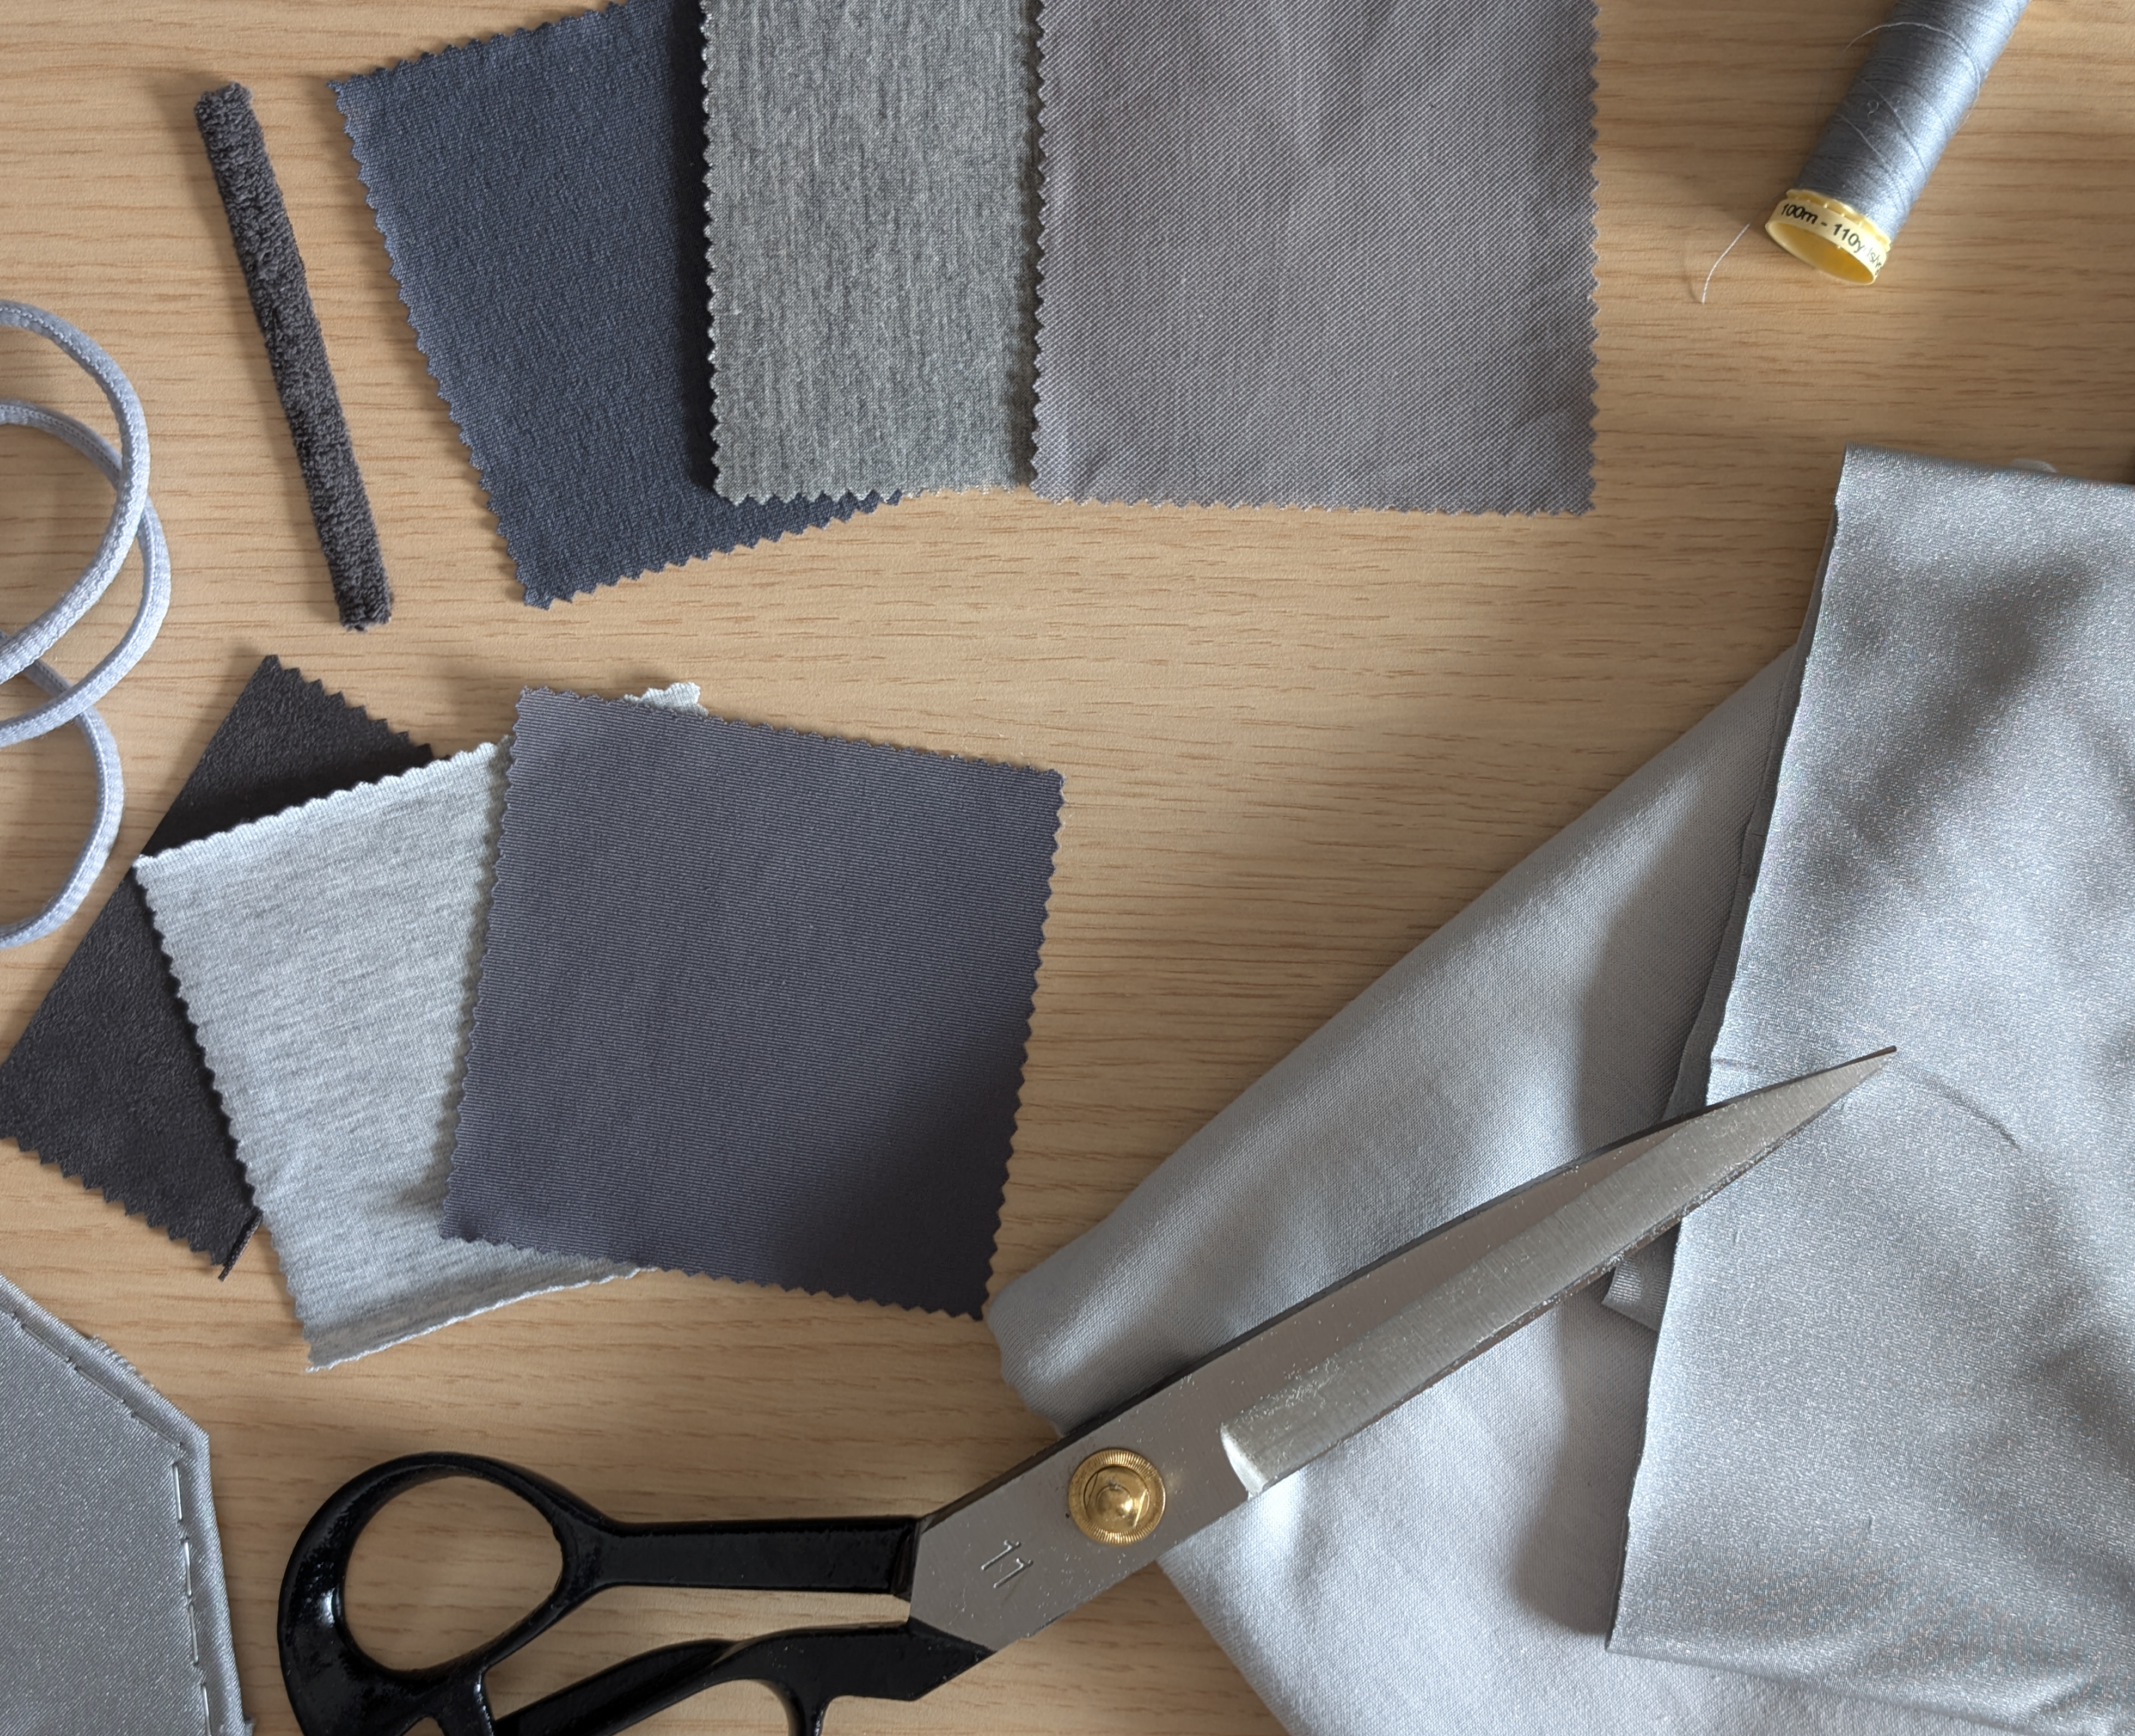
\includegraphics[width=1\linewidth]{images/Fabric Exploration.png}
    \caption{A broad sample of fabric was explored to identify a material that meets all requirements.}
    \label{fig:fabric-exploration}
\end{figure}

A separate, more detailed material exploration was conducted for the \textbf{volume slider} . While its long rectangular shape already affords a linear sliding gesture \cite{mlakar_design_2020}, the goal was to use the fabric itself to strengthen this affordance by leveraging the principles of signifiers \cite{mlakar_signifiers_2025}. 
% Guided by Mlakar et al.'s (2021) work, a \textbf{Textile Signifier} was created through material contrast. A cord fabric with a distinct directional nap was chosen for the slider. This "hairy" texture provides low resistance when swiped in the direction of the nap and higher resistance against it, strongly suggesting horizontal movement. 
Inspired by the principle that some textiles can create directional friction \cite{mlakar_exploring_2021}, a corduroy fabric with a distinct nap was selected. The fine "hairs" of the fabric were oriented to create a metaphor of resistance: sliding in one direction felt slightly different than sliding in the other, creating an intuitive link to the concepts of increasing and decreasing a value. This choice also created multiple layers of inherent feedforward cues. The texture itself acted as a \textit{Textile Signifier} \cite{mlakar_signifiers_2025}, creating a tactile and height contrast with the smooth base fabric, indicating the interactive nature of the slider, thus guiding the user where to interact. The nap also functioned as a \textit{Staging Signifier} \cite{mlakar_signifiers_2025}, as the unsettled portion of the fabric visually indicated the slider's current position and signified the direction it could be moved. Finally, several \textit{Visual Signifiers} \cite{mlakar_exploring_2021} were designed to reinforce the interaction, following the principle that users often assess an interface visually before touching it \cite{mlakar_exploring_2021, mlakar_signifiers_2025}. The slider was divided into sections that gradually increase in size from left to right, creating a clear visual metaphor for increasing a value (see Fig. \ref{fig:volume-slider-v1}). 
% While primarily affordance-clarifying, this graded division is also slightly function-revealing, though the specific function (e.g., volume) is not explicit from the form alone. 
This graded division adds a layer of function-revealing feedforward by clearly communicating the directionality of control. However, the cue remains generic, as it does not specify the particular function, such as volume, that is being adjusted. 
% The slider was given a darker color for visual contrast, a slightly slanted shape to emphasize horizontal motion, and internal divisions that gradually increase in size to afford the concept of "increase" toward the right.


\begin{figure}[H]
    \centering
    \includegraphics[width=1\linewidth]{images/Textile Prototype/Volume Slider V1.png}
    \caption{The volume slider design, using corduroy fabric to create directional friction. The gradually increasing segments act as a Visual Signifier for increasing a value from left to right.}
    \label{fig:volume-slider-v1}
\end{figure}


 The \textbf{pullable element for the "home" function} was realized as a physical cord, stitched into a loop. The loop shape acts as a strong signifier, inherently affording the action of being pulled up by a finger \cite{mlakar_signifiers_2025}. The loop expands over a width of approximately 45 mm, providing ample space for a finger to slide underneath, while the 5 mm diameter of the slightly squishy yet robust cord communicates durability. This element's state is also a key feedforward channel. Inspired by the concept of \textit{Staging Signifiers} by Mlakar et al. \cite{mlakar_signifiers_2025}, the loop's position indicates the system state. When a user navigates away from the main menu, a motor retracts the loop, making it flush with the surface and signifying that it can be pulled "up" again to return home (see Fig. \ref{fig:home-loop-v1}a). Conversely, when the main menu is active, the loop remains in its raised position (see Fig. \ref{fig:home-loop-v1}b), indicating that the action is complete and cannot be performed again.

 \begin{figure}[h!]
     \centering
     \includegraphics[width=1\linewidth]{images/Home Loop V1 small.png}
     \caption{The state of the "home loop" acts as a Staging Signifier. (a) In its retracted position, the loop signifies that it can be pulled up to open the main menu. (b) Once pulled, the loop remains raised while the main menu is active, indicating the action cannot be performed again.}
     \label{fig:home-loop-v1}
 \end{figure}
 

The \textbf{rotary dial} was implemented as a recessed circular groove with a depth of 3 mm (see Fig. \ref{fig:rotary-dial}), following recommendations from Nowak et al. \cite{nowak_shaping_2022}. This physical channel was designed not only to guide the user's fingertip for potential eyes-free use but also to visually afford a continuous circular motion, a principle supported by multiple studies \cite{dong_disappearing_2019, mlakar_design_2020, nowak_shaping_2022}. 
Within this dial, the central \textbf{tap surface} for confirmation actions was placed. This surface had a diameter of 35 mm as the comfort for the rotary gesture around it was prioritized. While a small enclosed shape generally affords a pressing gesture \cite{mlakar_design_2020}, it's size presented a potential pitfall as the surface is significantly larger than a fingertip. As Mlakar et al. \cite[pp.~1165]{mlakar_exploring_2021} pointed out; "If an element is circular and roughly the size of a fingertip, it affords pressing and will likely be assumed as a button [...]. If the circle is bigger, it becomes less clear whether the user is supposed to slide around the edge or press [...]”.  This potential ambiguity was to be validated in the subsequent user tests. To ensure this primary button was always locatable, its circular boundary was permanently marked with stitching, keeping it visible even when the surrounding dial groove was retracted and flush with the surface. 

\begin{figure}[h!]
    \centering
    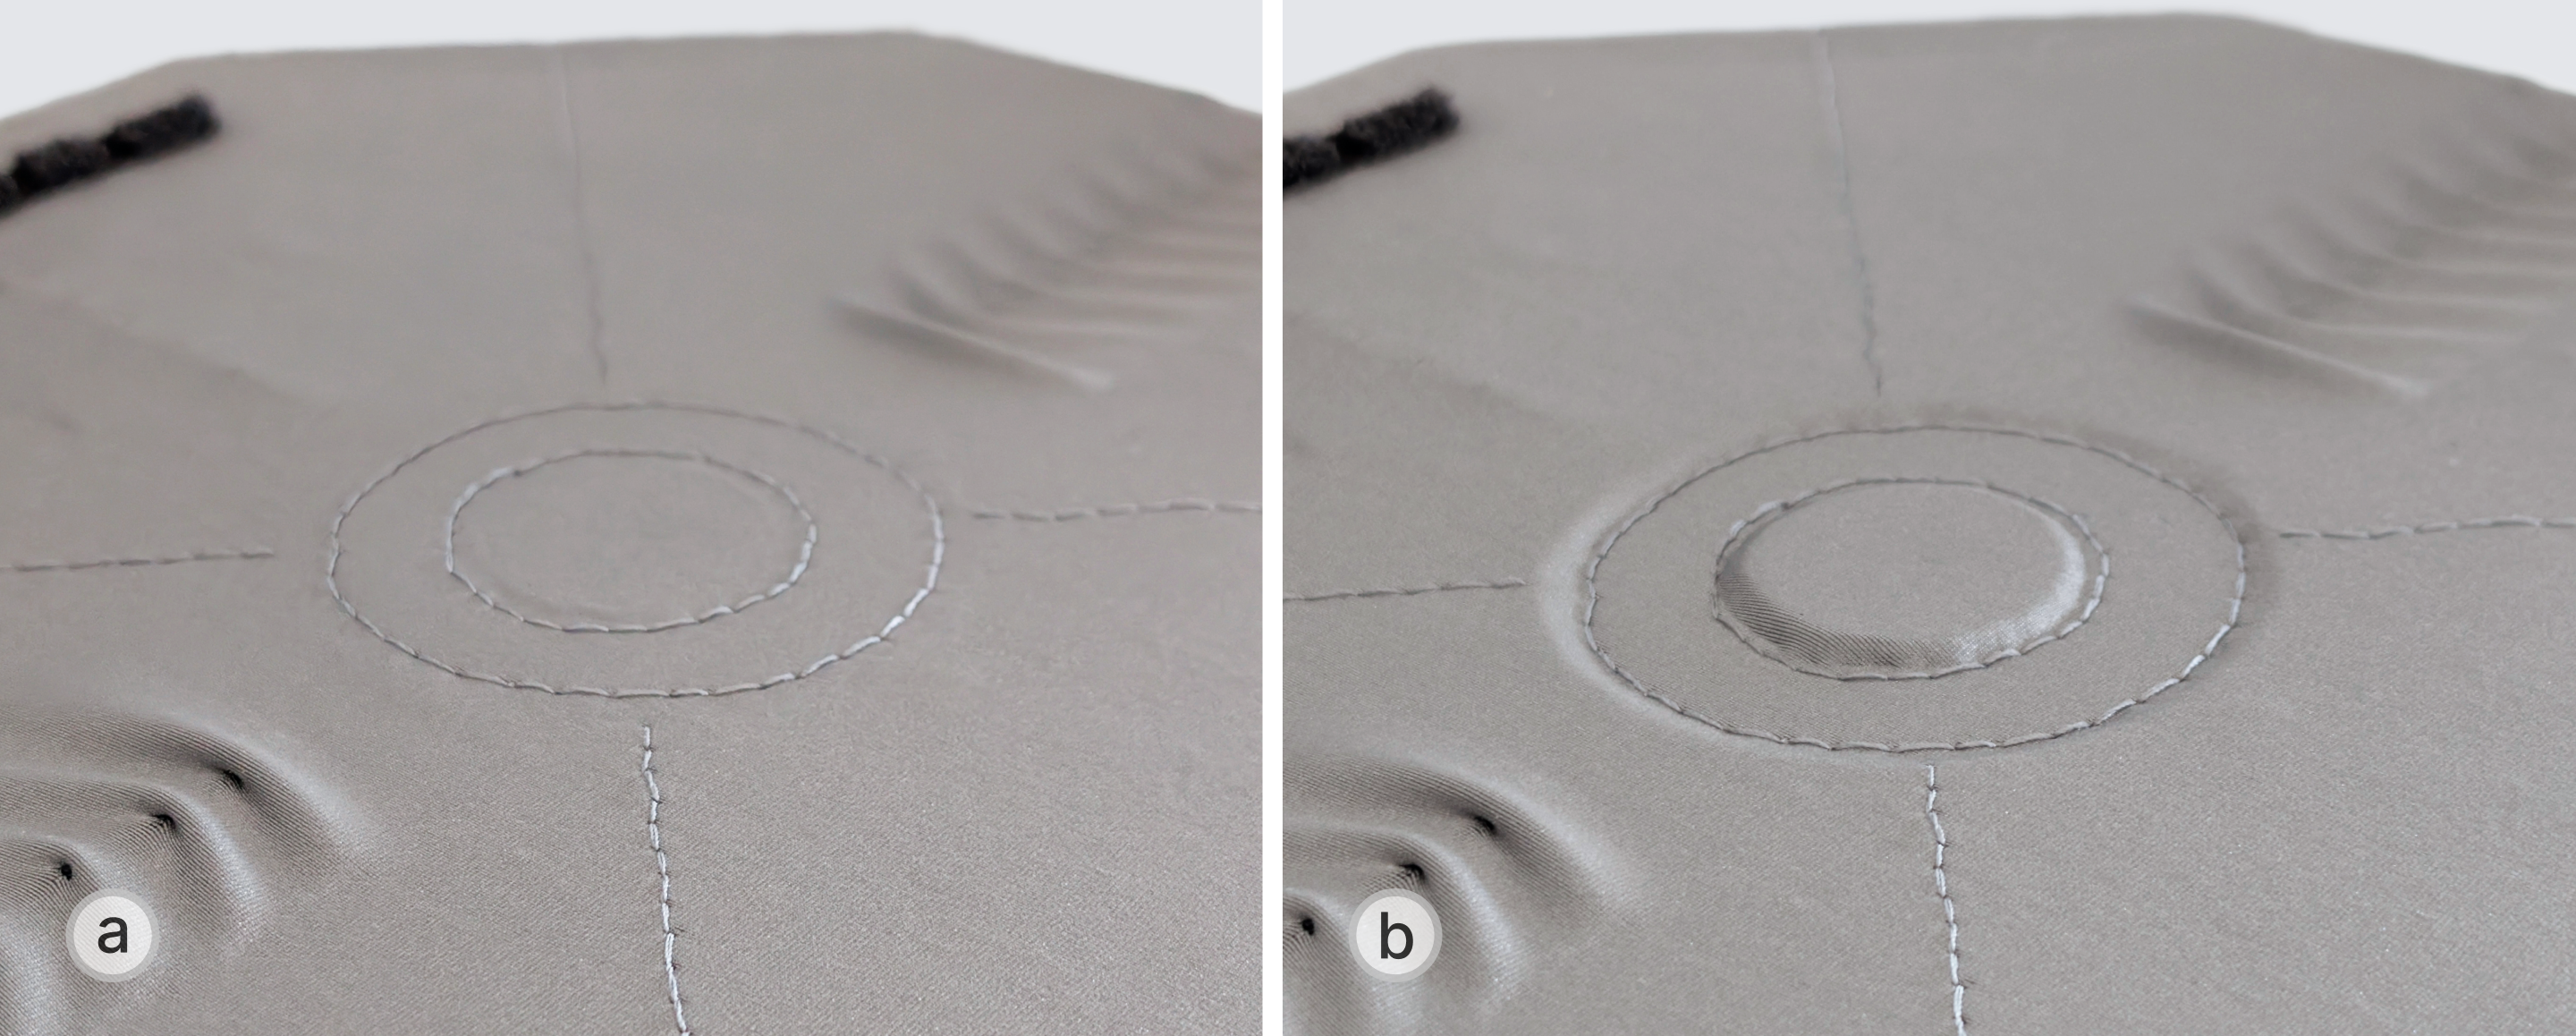
\includegraphics[width=1\linewidth]{images/Rotary Dial small.png}
    \caption{The shape-shifting rotary dial and central tap surface. (a) In its inactive state, the dial is flush with the surface, with permanent stitching marking the boundary of the tap area. (b) When active, the dial forms a recessed groove to guide the user's finger in a continuous circular motion.}
    \label{fig:rotary-dial}
\end{figure}

% The central confirm/select function was designed as a large tap surface with a 35 mm diameter, located within the rotary dial. Following the principle that a circle roughly the size of a fingertip affords pressing, this large surface was designed to afford a simple tap, without requiring the system to distinguish between different numbers of fingers. The circular outline of this tap area remains permanently visible via its stitched border, even when the rotary dial's groove is hidden.

The \textbf{directional swipe areas} make significant use of the fabric's deformability to create clear, unambiguous cues. The design goal was to create a surface that specifically affords a swipe in one direction only. To achieve this, a pleating texture was chosen, as this has been found to be a strong signifier for stroking or stroking gestures \cite{jiang_gesfabri_2022} (see Fig. \ref{fig:directionaö-swipe-areas-v1}c). 
However, to clarify the directionality, the shape-shifting mechanism itself was designed as a story telling \textit{Staging Signifier} \cite{mlakar_signifiers_2025}. The pleats are formed by pulling the fabric from underneath along a straight line of pulling-points; the observable direction of this tension indicates the intended gesture path. This also creates a \textit{Visual Signifier} \cite{mlakar_signifiers_2025}, as the pleats have a slightly pointy character, akin to an arrow (see Fig. \ref{fig:directionaö-swipe-areas-v1}b), indicating the intended direction of interaction \cite{mlakar_exploring_2021}. Based on an analysis of the system's functionalities, it was noted that the left and right directional swipes are always used as a pair; therefore, their corresponding pleats were connected to a single motor to appear and disappear together. The top swipe surface, however, is activated independently by a separate motor as needed.

\begin{figure}[h!]
    \centering
    \includegraphics[width=1\linewidth]{images/Directional Swipe Areas V1.png}
    \caption{The directional swipe areas in their two primary states. (a) A completely flat plane for 2D pointing tasks. (b, c) When activated, the fabric forms pleated guides that serve as visual and tactile signifiers for a directional swiping gesture.}
    \label{fig:directionaö-swipe-areas-v1}
\end{figure}

% Finally, a deliberate decision was made regarding the large \textbf{2D plane used for pointing tasks} (e.g., the POI or soundscape applications). No additional inherent physical cues were added for this mode, as they could interfere with the tactile cues of the other elements when the surface is in a different state. For this specific function, the system relies on the visual feedforward from the WSD's graphical user interface to suggest and guide the pointing interaction. This is a common strategy when a single physical surface must support multiple, distinct interaction models.

Finally, for the large \textbf{\gls{2D} pointing plane} used in tasks like the \gls{POI} selection, a conscious decision was made to not add any permanent inherent cues like a grid texture (see Fig. \ref{fig:directionaö-swipe-areas-v1}a). This was to avoid creating conflicting tactile information that could interfere with the other dynamic elements when they are active on the same surface. 
Instead, the design relies on two sources of feedforward: visual guidance from the \gls{WSD}'s \gls{GUI} to suggest the pointing task, and the inherent affordance of the surface itself. 
It was hypothesized that a completely flat and uniform plane could naturally communicate that the entire area is a single, continuous space available for interaction, an assumption to be evaluated in the subsequent user tests. 

Across all of these elements, two overarching principles guided the design. First, following the recommendation to design all shapes as simple as possible \cite{mlakar_design_2020}, the interactive zones were based on simple geometric forms like circles and lines. Second, a principle of economical use of signifiers was applied. While multiple layers of cues (Visual, Textile, and Staging) were often combined to strengthen an affordance, care was taken to avoid redundancy and unnecessary complexity, in line with suggestions that an "economic usage" of signifiers leads to better understanding of the interface \cite{mlakar_exploring_2021, mlakar_signifiers_2025}. The ultimate goal of this clear and economical design approach was to create perceptible affordances that were unambiguous to the user, thereby avoiding the usability pitfalls of hidden or false affordances \cite{gaver_technology_1991}.

\subsubsection{Designing the \gls{WSD}'s Graphical User Interface (\gls{GUI})}

The design of the \gls{WSD}'s Graphical User Interface (\gls{GUI}) was guided by the philosophy of creating an unobtrusive system that seamlessly integrates with the vehicle's interior and the outside view. The goal was to avoid a visually disjointed or "stuck-on" feeling, instead crafting a soft, organic interface that aligns with the "living space" concept and feels like a natural part of the environment.

\begin{figure}[h!]
    \centering
    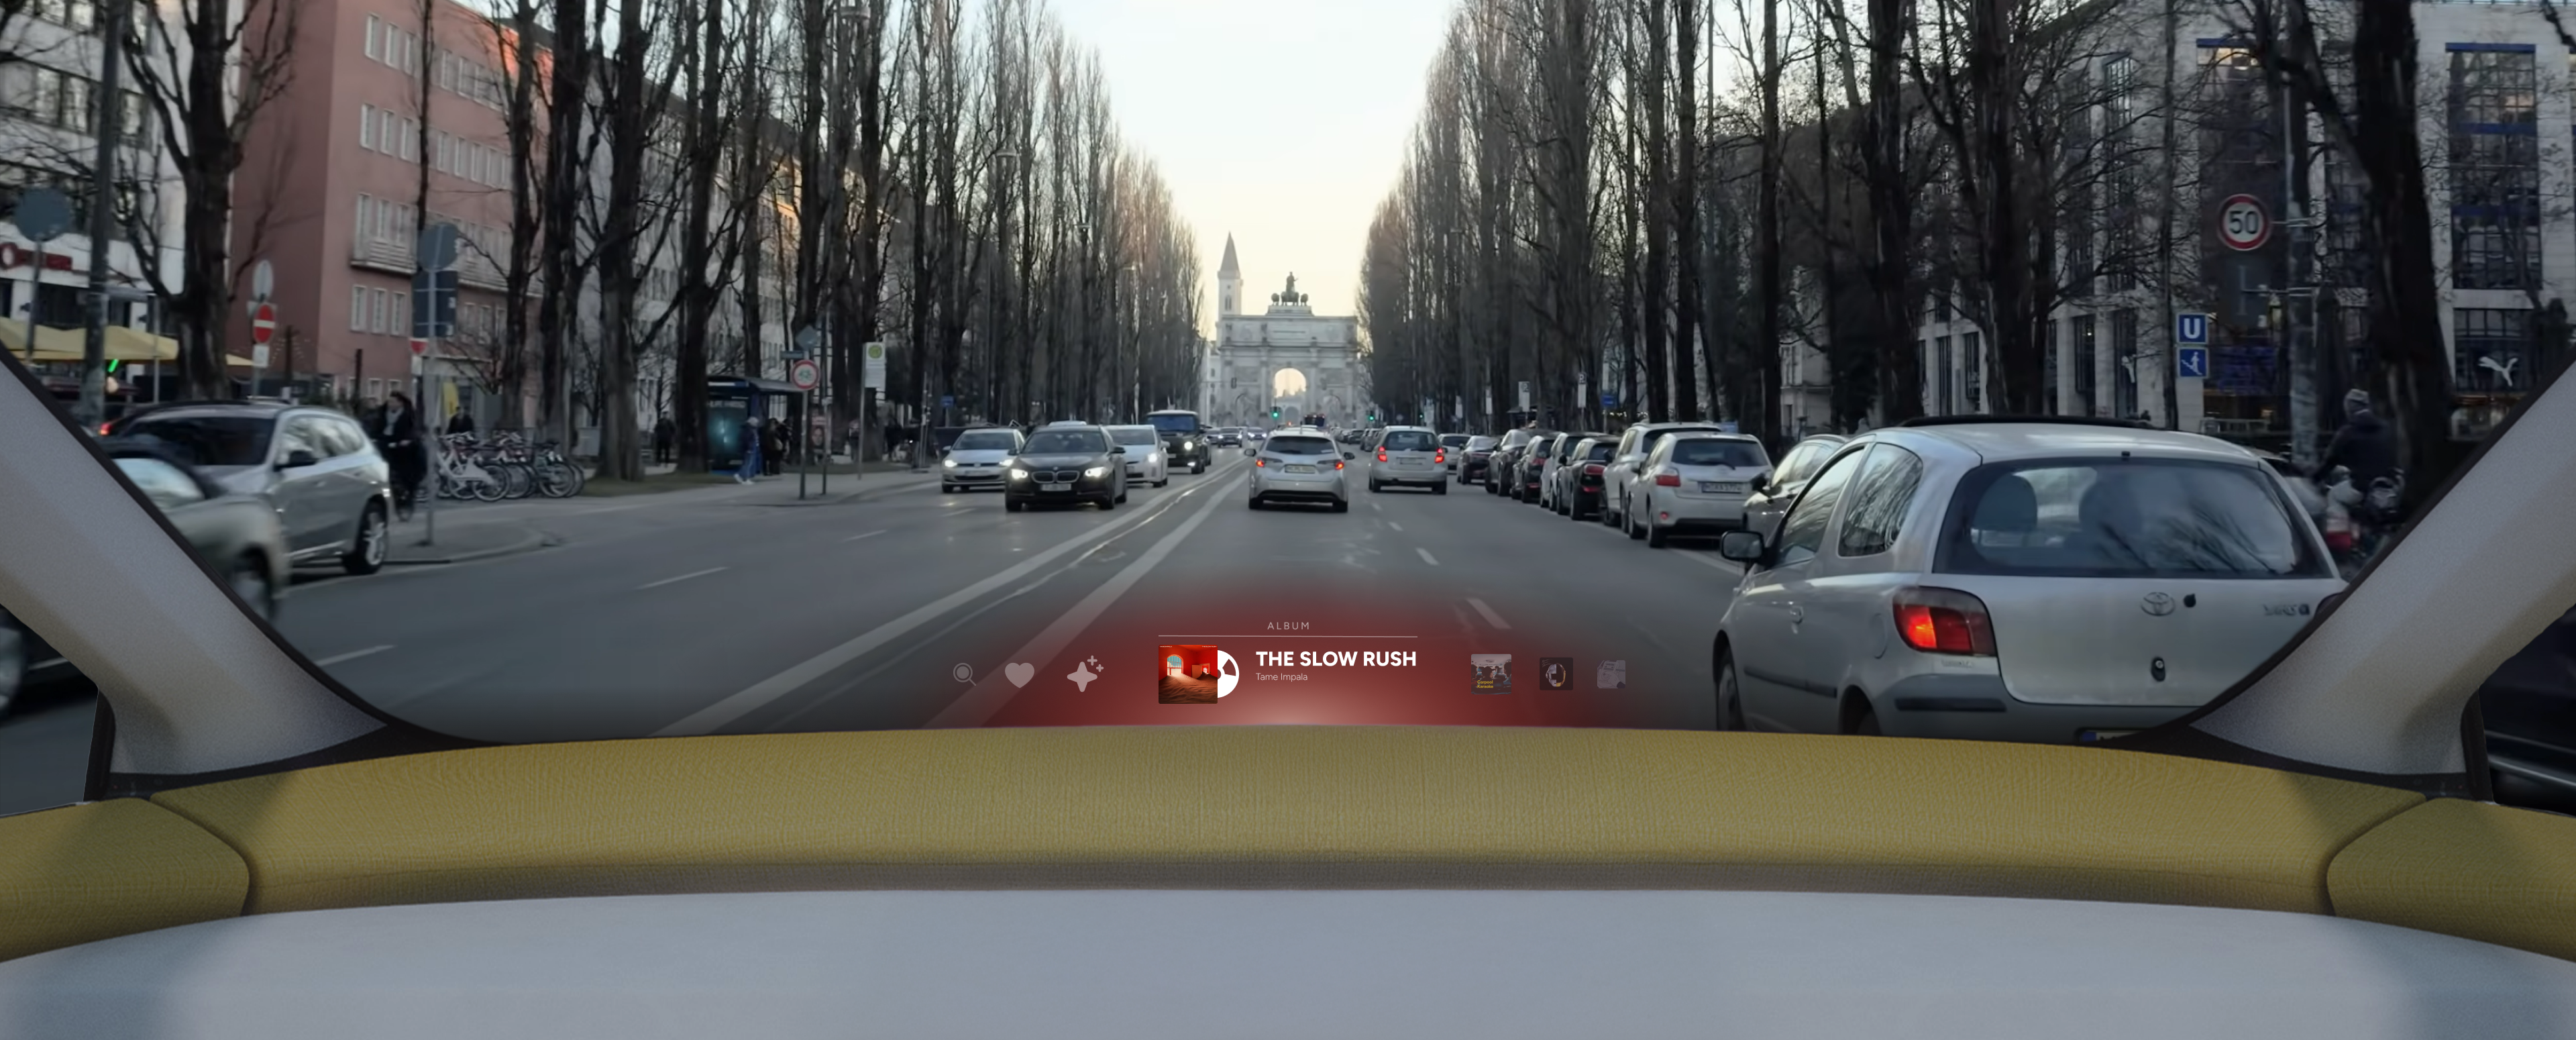
\includegraphics[width=1\linewidth]{images/Music - THE SLOW RUSH.png}
    \caption{Music Player Application, Example to show the UI located at the bottom of the \gls{WSD}, as to not obstruct the view.}
    \label{GUI-location-WSD}
\end{figure}


The layout and information hierarchy were designed to be intuitive and to complement the physical textile controller. The majority of \gls{UI} elements are displayed centrally at the bottom of the \gls{WSD}, appearing to hover over the vehicle's dashboard (see Fig. \ref{GUI-location-WSD}). This placement ensures that the \gls{GUI} occupies the view of the road immediately ahead but does not obstruct the user's view of the surrounding landscape. While research has shown a preference for landscape-oriented windows \cite{riegler_augmented_2019}, the design abandoned hard rectangular shapes in favor of soft, rounded, and elliptical forms. These shapes gradually fade into the background at the edges, creating a less intrusive feel. A core principle was maintaining a strong \textbf{spatial mapping} between the on-screen layout and the physical textile interface. For example, in the home menu (see Fig. \ref{fig:GUI-layout-examples}a), the centrally highlighted menu item corresponds to the central tap surface, while other items are arrayed horizontally around it, aligning with the left and right directional swipe areas. This principle is also evident in selection prompts, where options appear as movable "marbles" around a central selection (see Fig. \ref{fig:GUI-layout-examples}b); the user physically swipes the desired marble into the center of the screen, mirroring the action on the textile surface. Likewise, when the rotary dial is active, \gls{UI} elements are arranged in a circle, such as the contacts list that emulates a rotary phone (see Fig. \ref{fig:GUI-layout-examples}c) or the image of a vinyl record in the music player that can be "spun" to seek through a track (see Fig. \ref{fig:GUI-layout-examples}d).


\begin{figure}
    \centering
    \includegraphics[width=1\linewidth]{images/GUI-layout-examples.png}
    \caption{\gls{GUI} design samples illustrating the system's core interaction metaphors: (a) horizontal list navigation in the home menu, (b) the "marble" selection metaphor, (c) a rotary layout for the contacts list, and (d) the "spinning vinyl'" metaphor for media control.}
    \label{fig:GUI-layout-examples}
\end{figure}


The visual design was crafted to be both aesthetically pleasing and highly functional. Instead of solid colors, the background of each application consists of soft gradients, rather than solid colors, that reflect the dynamic blending of colors of the scenery outside the \gls{WSD}, with each application having a unique gradient for clear identification. These gradients are also dynamic; for example, accepting a call by selecting the green "marble" causes the background to bloom into a corresponding green gradient as feedback, indicating a now active call. 
To maintain legibility while blending with the environment, all background elements had an 80\% opacity that faded out at the edges. To ensure contrast against varying external conditions, this was overlaid on a semi-transparent black background field (40\% opacity), a practice supported by the findings of Riegler et al. \cite{riegler_adaptive_2019}. 
% The main GUI elements are rendered at 80\% opacity and fade at the edges, supported by a semi-transparent (40\% opacity) black background area that also fades out, ensuring legibility without being obtrusive, in line with findings from Riegler et al. (2019). 
Typography was built on a clear hierarchy using the sans-serif font Figtree \cite{kennedy_figtree_nodate}. Prominent text is bold, while secondary information uses variations in font weight and transparency. All text is white to maintain contrast against the dynamic backgrounds. For iconography, the clear, minimalist, open-source Phosphor icon pack \cite{fried_phosphor_nodate} was used.

Finally, motion design was a critical channel for feedforward, used to make the interface feel alive and to guide interaction. The very first interaction on the welcome screen is a pulsing circles designed to look like water ripples (see Fig. \ref{fig:welcome+spotlight}a), directly mirroring the circular stitching on the physical prototype and affording a touch to "start" the system. Other dynamic cues were used throughout: the selected item background in the main menu has a subtle "breathing" animation to afford a tap; the "marbles" in a selection prompt animate from the center outwards when they appear, showing their potential trajectory back to the center; and when opening an album in the music player, the vinyl record icon animates out of the album cover art with a slight spin, suggesting the rotational gesture that controls it. 
Similarly, for the \gls{2D} pointing task in the Point of Interest (\gls{POI}) function, a spotlight-shaped cursor (see Fig. \ref{fig:welcome+spotlight}b) appears and subtly moves around the center of the screen, mimicking an eye scanning the scenery. This initial, autonomous movement acts as a critical feedforward cue, signifying that the cursor is a dynamic, draggable element that the user can control, rather than a static icon.
% These microinteractions were designed to make every touch feel responsive and to intuitively communicate how the interface could be used.

\begin{figure}[h!]
    \centering
    \includegraphics[width=1\linewidth]{images/Welcome+Spotlight.png}
    \caption{The use of dynamic cues as feedforward to guide interaction. (a) A pulsing ripple animation on the welcome screen invites a "start" touch. (b) The autonomous movement of the spotlight cursor upon opening the app signifies its draggability for selecting the nearby POI.}
    \label{fig:welcome+spotlight}
\end{figure}

These dynamic cues were part of a broader strategy to follow the principles of a Natural User Interface, or \gls{NUI} \cite{wigdor_brave_2011}, where every physical interaction elicits an immediate, corresponding, and natural-feeling reaction from the \gls{GUI}. For example, turning the physical dial causes the on-screen element to rotate accordingly, and swiping a "marble" on the textile surface results in its digital counterpart fluidly moving into the central selection zone, making the tangible interaction feel both intuitive and directly manipulative. 

\subsubsection{Defining Feedforward Levels for Evaluation}
% This is the perfect place to explain the 'why' and 'what' of your study's core conditions, as you have just defined the baseline: Inherent Cues.

To systematically investigate the research gap concerning intuitive interaction, three distinct levels of feedforward were defined for evaluation. This approach allows for a controlled comparison, as each level builds upon the same physical prototype and baseline \gls{GUI}. The conditions were not chosen at random; they were deliberately designed to represent three distinct and representative points on the Feedforward Matrix, spanning a spectrum from purely physical, inherent cues to progressively more augmented and function-revealing forms of guidance (see Fig. \ref{fig:success-rates-condition}). This strategy allows for a meaningful analysis of how different feedforward philosophies impact the user experience.

\begin{figure} [h!]
    \centering
    \includegraphics[width=1\linewidth]{images/Feedforward Matrix/Feedforward Matrix Conditions V2.png}
    \caption{Feedforward Matrix, visualizing the feedforward conditions: (a) Inherent Cues, (b) Augmented Light Cues, and (c) Augmented Text Cues.}
    \label{fig:feedforward-matrix-conditions}
\end{figure}

\paragraph{Condition 1: Inherent Cues (Baseline):}

This condition represents the purest form of physical guidance and serves as the experimental baseline. It relies solely on the inherent feedforward cues designed into the prototype's physical form, as detailed in the previous section \ref{inherent-feedforward}. Users receive guidance only from the shape, texture, position, and deformability of the textile elements.

On the Feedforward Matrix, this condition occupies the top-left end of the axes (see Fig. \ref{fig:success-rates-condition}a). Its cues are fully embedded in the material and are almost exclusively Affordance-Clarifying, designed to answer the question, "What can I do and how?" through tactile and physical properties alone.

\paragraph{Condition 2: Augmented Light Cues:}
This condition explores a subtle, seamlessly integrated layer of augmentation by adding dynamic light projections directly onto the textile surface. A key strength of these projections is the ability to reinforce the directionality of an interaction through subtle animations that guide gestures, clarifying how to interact. For instance, soft swipe animations moving along the physical pleats of the directional swipe areas add another layer of guidance on top of the inherent physical cues (see Fig. \ref{fig:arrow-dial-lc}). The light cues also allow for easy integration context-dependent affordances. For example, while the physical rotary dial affords rotation in both directions, a light animation, such as a glowing circle accelerating repeatedly in one direction, can signify that, in the current context (e.g., at the beginning of a list), only a single direction of rotation is possible.


\begin{figure}[h]
    \centering
    \includegraphics[width=1\linewidth]{images/ArrowDialLC.jpg}
    \caption{The seamlessly integrated augmented light cues during music playback. Animated arrows on the pleated surfaces guide swipe gestures, while a rotational cue on the dial affords playback control.}
    \label{fig:arrow-dial-lc}
\end{figure}

% Beyond these affordance-clarifying abilities, the light cues also have potential to hint at the interaction's function through the use of color, creating a direct visual link to UI elements on the WSD. This allows for easy mapping between the GUI and the physical controls, clarifying what a gesture will result in. For instance, the light projected onto the three directional swipe areas would match the colors of the corresponding "marble" options displayed on the screen. Critically, the light projections also serve to establish the initial connection between the WSD and the textile controller for a first-time user. On the welcome screen, the pulsing "water ripple" animation on the WSD is mirrored by a light projection on the textile surface, strongly affording a touch in the center while simultaneously linking the two interfaces.

Beyond clarifying affordances, the light projections also served to communicate the system's current state and the availability of controls. While the dynamic elements on the textile surface use shape-shifting to signal their availability, the light projections add this dynamic layer to the static elements, such as the volume slider and home loop. The light can display the current state of a control, for example by illuminating a portion of the slider to represent the current volume level. It can also signify when a static element is interactive; the volume slider and home loop are only augmented by light when their functions are available in the current context, e.g. when there is active media playback. Furthermore, the use of dynamic color creates a direct visual link to \gls{UI} elements on the \gls{WSD}, which serves a function-revealing purpose by allowing for easy mapping between the \gls{GUI} and the physical controls. For instance, the light projected onto the three directional swipe areas would match the colors of the corresponding "marble" options on the screen (see Fig. \ref{fig:marble-lc}), clarifying the result of a user's action. Critically, the light projections also serve to establish the initial connection between the \gls{WSD} and the textile controller for a first-time user. On the welcome screen, the pulsing "water ripple" animation on the \gls{WSD} is mirrored by a light projection on the textile surface, strongly affording a touch in the center while simultaneously linking the two interfaces.

\begin{figure}[h]
    \centering
    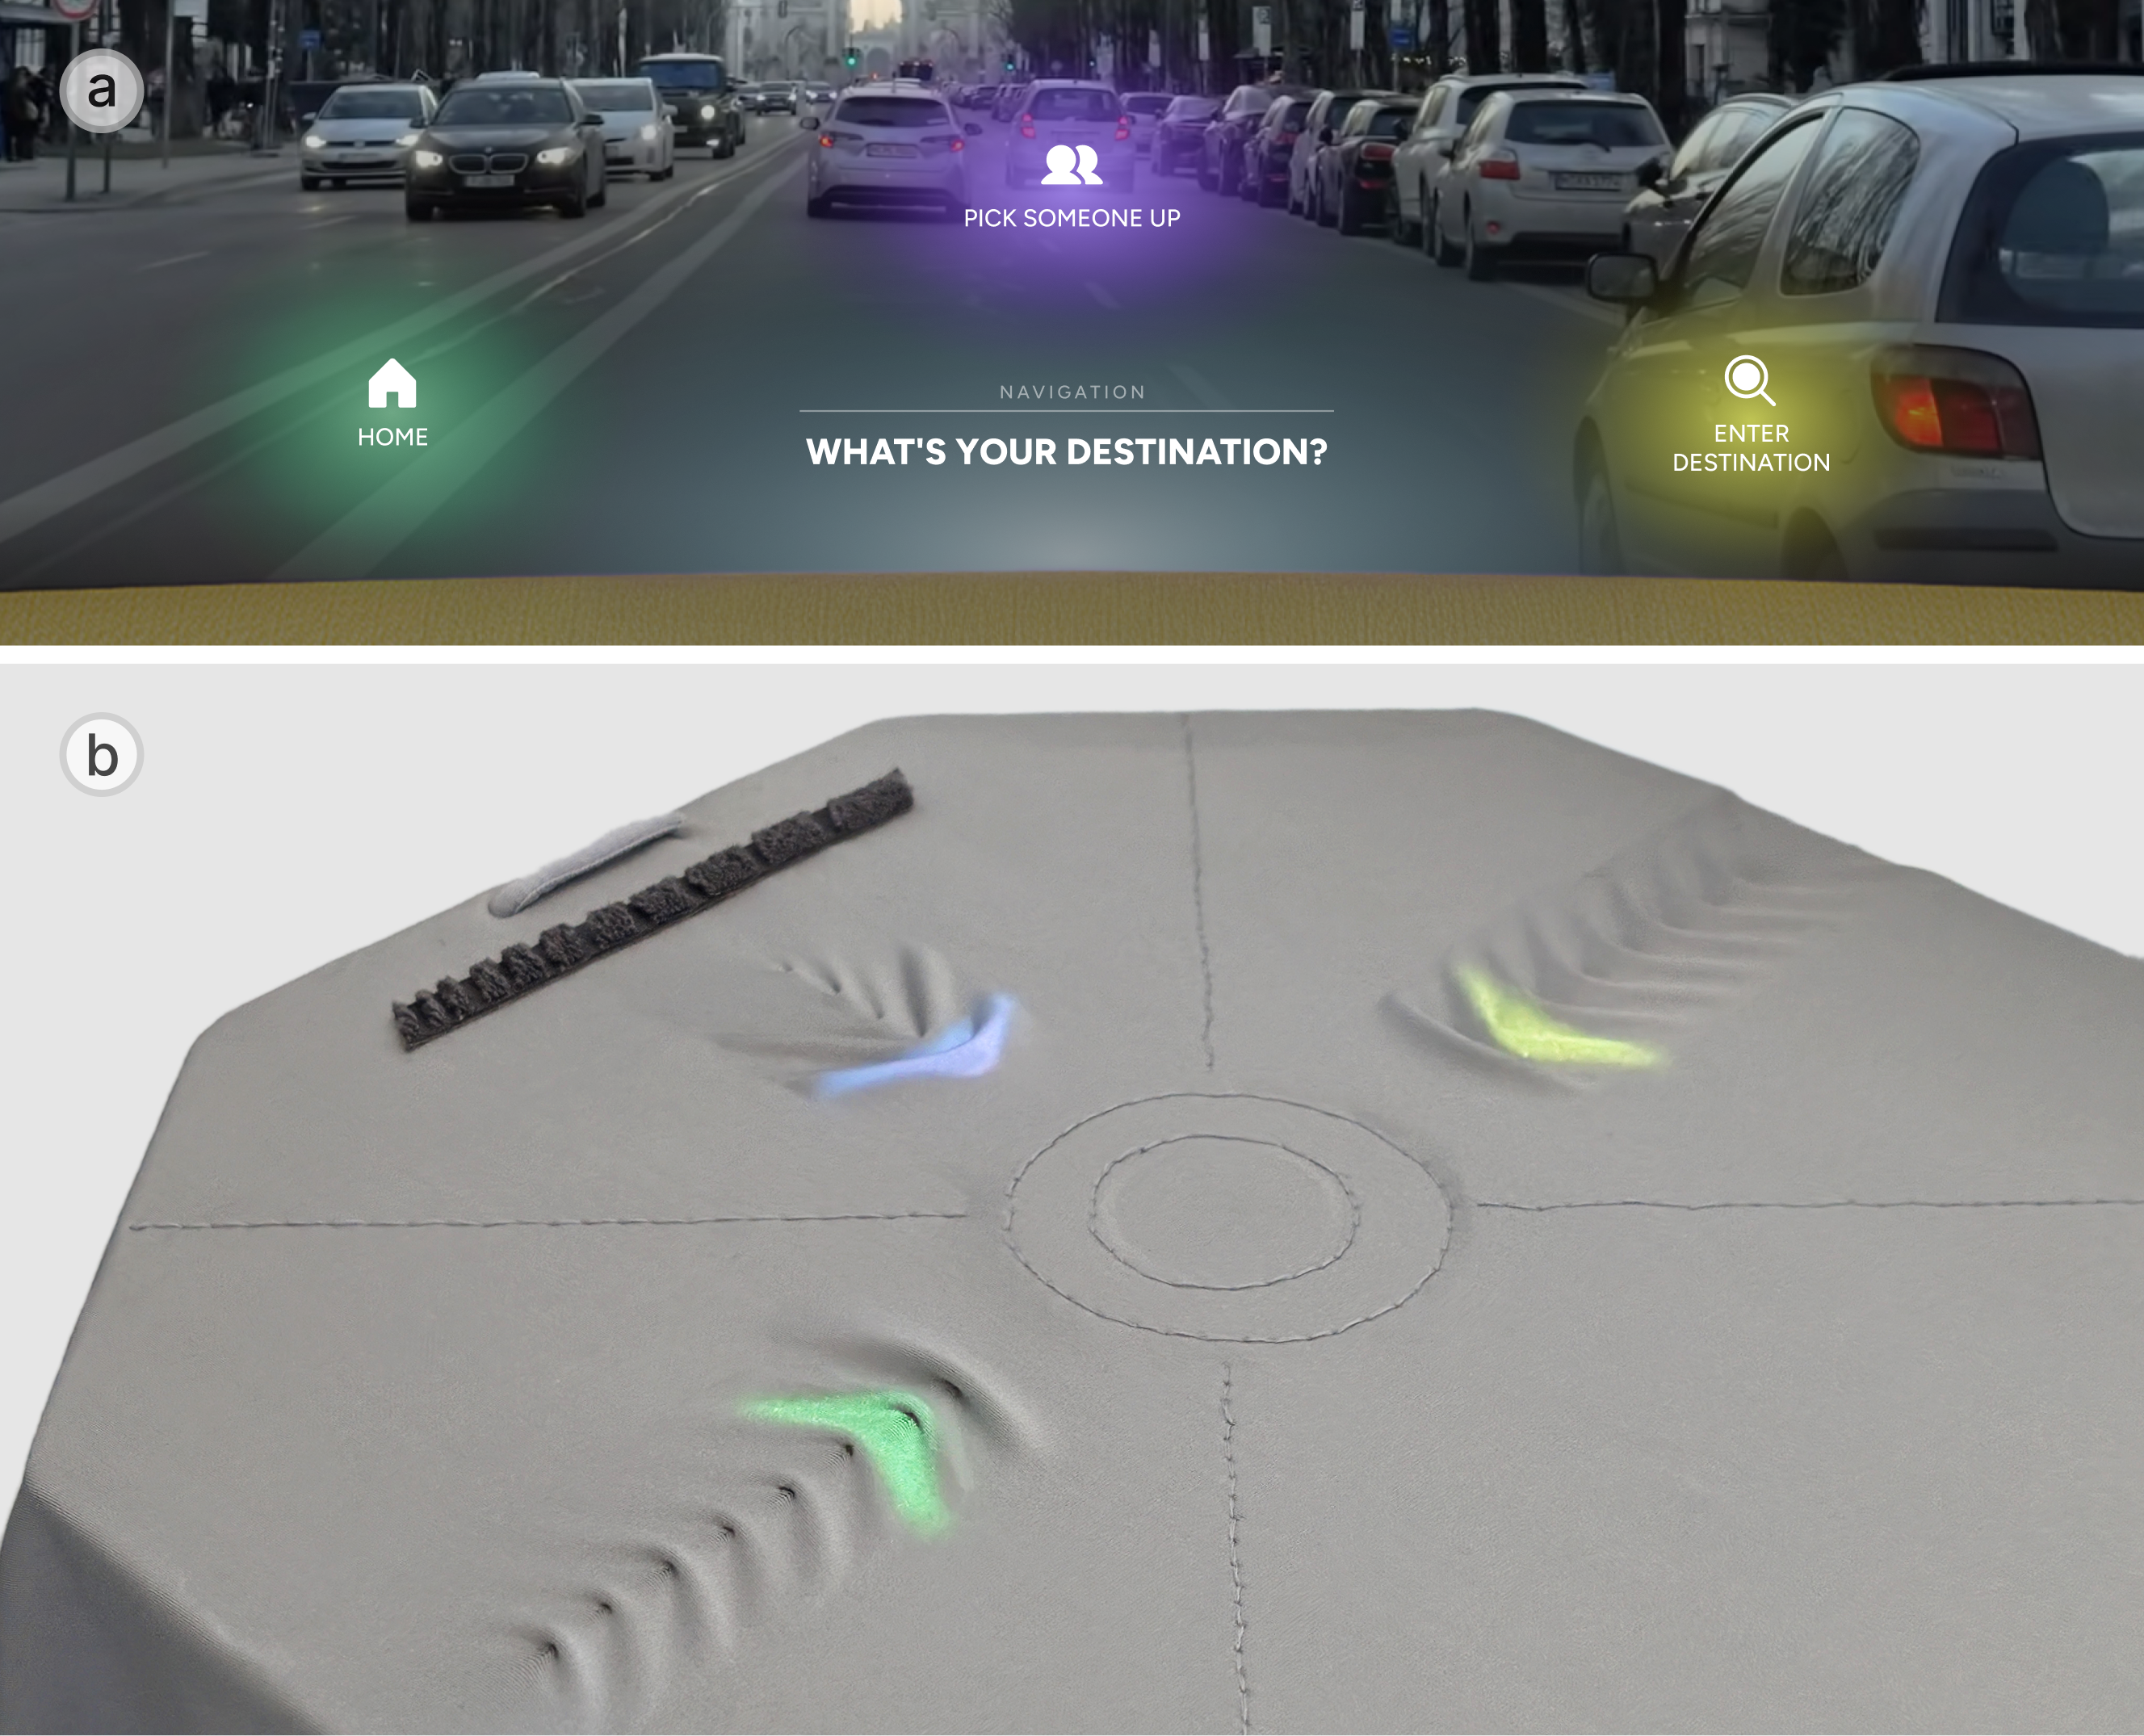
\includegraphics[width=1\linewidth]{images/Marble LC.png}
    \caption{The use of color-coded light cues to create a direct function-revealing mapping between the GUI and the physical interface. During the "marble" selection task, the colors of the on-screen options (top) directly correspond to the light projected onto the interactive textile areas (bottom).}
    \label{fig:marble-lc}
\end{figure}

The visual design of these cues aimed for a "shy" integration, with blurred edges, smooth animations, and projected shapes that precisely follow the physical form of the elements, allowing them to seamlessly blend into the fabric. On the Feedforward Matrix (see Fig. \ref{fig:success-rates-condition}b), this condition sits between fully Embedded and Augmented, leaning more towards Embedded due to its seamless integration. Informationally, it is mostly Affordance-Clarifying but also introduces Function-Revealing elements through its color mapping.


\paragraph{Condition 3: Augmented Text Cues:}
This condition investigates the effect of explicit, textual instruction by adding written hints directly into the \gls{WSD}'s \gls{GUI}. The aim was to be as unambiguous as possible about both the required action and its resulting function.

To integrate these cues in a predictable yet unobtrusive manner, they were given a single, consistent position at the bottom of the \gls{GUI} (see Fig. \ref{fig:text-cue-examples}). This placement ensures that a user seeking guidance always knows where to direct their gaze. The instructions followed a consistent formula, clearly stating which gesture leads to which function (e.g., "Tap to view forecast", "Swipe left to decline"). A key design challenge was balancing the need for these cues to be short and easily graspable with the risk of ambiguity that can arise from oversimplification. Another challenge was avoiding information overload in complex situations with multiple interaction possibilities, such as during playback in the media player. To solve this, a maximum of two cues were displayed side-by-side (see Fig. \ref{fig:text-cue-examples}b); if more instructions were needed, they would fade in and out in timed intervals to avoid overwhelming the user.

\begin{figure}[h]
    \centering
    \includegraphics[width=1\linewidth]{images/Text Cues Examples.png}
    \caption{Examples of the augmented text cues, designed for clarity and predictability. The cues appear in a consistent location at the bottom of the screen (a), with a maximum of two displayed side-by-side to explain multiple interaction possibilities, like an incoming call (b).}
    \label{fig:text-cue-examples}
\end{figure}

On the Feedforward Matrix (see Fig. \ref{fig:success-rates-condition}c), this condition is positioned towards the Augmented/External end of the integration axis, as the cues are integrated in the \gls{GUI}, physically distant from the textile controller. Informationally, it is a mix of Affordance-Clarifying (e.g., "spin clockwise") and Function-Revealing (e.g., "to fast-forward"), with a stronger emphasis on revealing the function, as the textual description of a gesture is more abstract than a physical or seamlessly integrated visual cue directly mapped on the surface.

% +++++++++++++++++++++++++++ ADD CONDITION MATRIX HERE +++++++++++++++++++++++++++++++++++++

\subsubsection{Scenario Selection and Storyline Creation}

\paragraph{Defining the Scope of the Study:} \mbox{} \\
From the full set of designed \gls{NDRA}s, it was necessary to select a representative subset for full implementation in the user study prototype. The primary criterion for this selection was the need to maximize the diversity of interaction types to ensure that the full range of the prototype's capabilities was thoroughly evaluated. Specifically, the selection was guided by the need to include examples of all the core interaction primitives designed for the textile surface: simple \textbf{taps} for selection, \textbf{linear continuous input} (volume slider), \textbf{rotary continuous input} (dial), \textbf{directional swipes} for choices and menu navigation, the textile-specific \textbf{pull gesture} for the home menu, and the \textbf{\gls{2D} pointing plane}.

To cover these varied interactions, a set of functions and applications was chosen for implementation. This included an essential ride-starting sequence composed of a \textbf{welcome screen} and \textbf{navigation prompts} (for destination and route confirmation). In addition, a suite of common in-vehicle applications was implemented, reflecting some of the most frequently cited \gls{NDRA}s for future \gls{AV}s. This selection included a \textbf{Music Player} to support leisure and entertainment needs \cite{ahram_what_2020, large_design_2017, pfleging_investigating_2016, wilson_non-driving_2022},  and a \textbf{Phone/Call system} with contacts and messaging to support the critical roles of communication and productivity \cite{ahram_non-driving_2020, large_design_2017, pfleging_investigating_2016, wilson_non-driving_2022}. Finally, the novel \textbf{\gls{POI} Spotlight application} was included to directly enhance the common activity of looking out the window \cite{berger_designing_2021, ahram_what_2020, pfleging_investigating_2016, stampf_deriving_2024} by augmenting the view with enriching information, a key potential for \gls{WSD}s identified in the literature \cite{berger_designing_2021, haeuslschmid_first_2016, matsumura_active_2018, pagura_window_2011}. This curated set of tasks ensured that every designed interaction primitive would be evaluated within a contextually relevant and well-justified application.

\paragraph{Creating the User Experience:} \mbox{} \\
\begin{comment}
% A cohesive storyline connecting these interactions into four distinct scenarios ("Welcome", "Music", "Spotlight", and "Call") was created.
% This narrative approach was designed to help participants in the user test vividly imagine the context of use and experience the prototype in a more immersive and engaging way. The main story line is that the participant is that they finished work and got to their car (a fully autonomous vehicle SAE level 5) in the parking lot. they now want to drive home.
% Scenario 1: Welcome: The journey begins with the 'Welcome' scenario. Upon entering the vehicle, the user is presented with the pulsing ripple on the \gls{WSD}, prompting their first interaction to 'start' the system. after that the system guides the user through a precess to start the drive with the AV, asking for the destination (participant has to select the home destination) then which route (user is free to choose from fastest, eco and scenic) and then view an overview of the journey ahead and confirm it to start the right. this introduction process that is required to start the drive with the vehicle as there are no manual driving controls on the other hand it is designed to carefully introduce the system to novice users without being annoying or slowing down expert users. for this we used the scaffolding design principle for NUIs proposed by Widgor and Wixon 2013. This prinicpile's goal is  "is that the user moves from "novice" to "expert" quickly and with pleasure. By novice we simply mean someone who uses the system for the first time. By expert we mean someone who uses the system in the way that the designers intended, feels pleasure in those activities, and has achieved that level of competence without the slow and tortuous learning that is typical of mastering many new interfaces".
% This scenario tests the crucial first steps of discoverability and walk-up-and-use(ability) since there is no explicit tutorial or onboarding teching process before the user can use the system (like that was the og research goal).
% Scenario 2: Music: After starting the drive home, the narrative continues with the user deciding to play music. The user is given a specific album name to find and to start playback of a song. Here another example of scaffolding can be found as upon opening an album the playback of the first song does not start immediately, however the user first has to give the vinly record displayed on the WSD a spin to start playback introducing the user to the methaphor and teaching that the rotary dial in this application is used to physically move the vinyl, thus allowing for interactions like fast forwarding or rewinding based on the spin direction, as well as pausing the playback by holding down the record, physically stopping it's movement and thus the playback. After starting the playback other tasks in this scenario include changing the volume, seeking in the song, skipping a song. Then the user does not feel like music anymore so they pausing the playback and returning back to the home menu.  idk what this scenario was made for in ters of what it can find out, i guess it's an example of a playful unconventional interaction methaphor from a music player which might have a good positive experience but also risks to be dificult to understand, however as described earlier one of the goals when design  the interface are these playful interactions and avoiding of just replicating interaction on the textile interface from it's digital counterparts.
% Scenario 3: Spotlight (POI): the vehicle is in some dense traffic with little movement, but since the user has not been in this part of town before they want to find out more about their surrounding, so they open  the 'Spotlight' application, it shows a total of three POI which can be selected by dragging the spotlight cursor around on the 2D pointing plane,. when the cursor gets close to POI it snaps onto the POI and after a short dwell time it opens a window with informations about the location like it's name, fun facts and opening times. int he scenario the user is interested to find out more about two buildings, after getting the information they leave the application and return to the home menu. idk what this scenario evaluates.
% Scenario 4: Call: "Finally, the user receives an incoming phone call from a coworker, they accept the call and get to know that the coworker has to cancel a meeting that was scheduled for tomorrow morning, they remember that another coworker called Daniel was also invited and ask the user to send them a short message letting him know the meeting is canceled , while the person on the phone says this the system is actively listening and giving the user matching information about the scheduled meeting. the person on the phone hangs up and the user has to message Daniel without further guidance. this requires opening the contacts lit, navigating through it with the rotary dial and finding and selecting daniel, the system displays infromation from the call the user just had signifying that the meeting with daniel should be cancled through a message, then through a series of promts the user can choose to send a message and sees two examples written by the system, they can choose any of their liking, after the message is sent they return to the home menu. This scenario was intentionally deigned to review all previously used interactive elements on the textile interface (except for the volume slider) but presenting these in diferent context, this is to evaluates if the user has sucessfully learned how the system works.
\end{comment}
To evaluate the prototype, a cohesive storyline was created that connects the various interactions into four distinct scenarios. This narrative approach was designed to help participants vividly imagine the context of use and experience the prototype in a more immersive and engaging way. The storyline places the participant in a fully autonomous, SAE Level 5 \cite{on-road_automated_driving_orad_committee_taxonomy_2021} vehicle after finishing work; their goal is to start a journey and drive home.

\subparagraph{Welcome Scenario}
The journey begins with the Welcome Scenario. Upon entering the vehicle, the user is presented with the pulsing ripple on the \gls{WSD}, prompting their first interaction to "start" the system. The system then guides them through a necessary ride-starting sequence: selecting a destination ("Home"), choosing a route ("Fastest", "Eco", or "Scenic"), and confirming the journey overview. This process was designed to be an intuitive introduction for novice users while remaining efficient for experts, following the scaffolding principle for \gls{NUI}s proposed by Wigdor and Wixon \cite{wigdor_brave_2011}. The goal of scaffolding is to help a user move from "novice" to "expert" quickly and pleasurably, without a slow or tortuous learning process. Therefore, this first scenario was designed to test the prototype's crucial discoverability and walk-up-and-use usability, as no explicit tutorial is provided before the user must successfully start their journey.

\begin{figure}[h!]
  \centering
  \label{ws1-welcome-scenario}
  \noindent\includegraphics[width=\linewidth]{images/Scenario Tables/WS-welcome-screen-row1.png}\\[-0.09em]
  \label{ws1-destination-selection}
  \noindent\includegraphics[width=\linewidth]{images/Scenario Tables/WS-destination-selection-row2.png}\\
  [-0.09em]
  \label{ws1-route-selection}
  \noindent\includegraphics[width=\linewidth]{images/Scenario Tables/WS-route-selection-row3.png}\\[-0.09em]
  \label{ws1-journey-confirmation}
  \noindent\includegraphics[width=\linewidth]{images/Scenario Tables/WS-journey-confirmation-row4.png}%
  \caption{Overview of the Welcome Scenario tasks and corresponding feedforward cues of prototype Version 1.}
  \label{fig:overview_welcome-scenario_version-1}
\end{figure}

\newpage
\subparagraph{Music Scenario}
After the drive home begins, the narrative continues with the user deciding to play music. They are tasked with finding a specific album, selecting it, and initiating playback. This scenario features another example of scaffolding: the music does not start automatically after selecting the album. Instead, the user is taught the interaction metaphor by being required to give the on-screen vinyl record a "spin" with the rotary dial to start the first song. This teaches them that the dial is physically mapped to the record, allowing for intuitive seeking by spinning and pausing by holding the dial to "stop" the record's movement. Subsequent tasks include changing volume and skipping tracks before pausing and returning home. This scenario was designed to evaluate the learnability and hedonic quality of a novel, physically-inspired metaphor, testing if a playful and unconventional interaction can be understood and enjoyed, in line with the design goal of avoiding mere replications of standard digital controls \cite{gowrishankar_strategy_2017}.


\begin{figure}[h!]
  \centering
  \label{ms1-navigate-home-menu}
  \noindent\includegraphics[width=\linewidth]{images/Scenario Tables/MS-navigate-home-menu-row1.png}\\[-0.09em]
  \label{ms1-open-music-app}
  \noindent\includegraphics[width=\linewidth]{images/Scenario Tables/MS-open-music-app-row2.png}\\
  [-0.09em]
  \label{ms1-navigate-music-menu}
  \noindent\includegraphics[width=\linewidth]{images/Scenario Tables/MS-navigate-music-menu-row3.png}\\[-0.09em]
  \label{ms1-open-album}
  \noindent\includegraphics[width=\linewidth]{images/Scenario Tables/MS-open-album-row4.png}\\
  [-0.09em]
  \label{ms1-start-playback}
  \noindent\includegraphics[width=\linewidth]{images/Scenario Tables/MS-start-playback-row5.png}\\[-0.09em]
  \label{ms1-adjust-volume}
  \noindent\includegraphics[width=\linewidth]{images/Scenario Tables/MS-adjust-volume-row6.png}\\
  [-0.09em]
  \label{ms1-rewind-track}
  \noindent\includegraphics[width=\linewidth]{images/Scenario Tables/MS-rewind-track-row7.png}\\[-0.09em]
  \noindent\includegraphics[width=\linewidth]{images/Scenario Tables/spare-footer.png}
  \caption{Overview (part one) of the Music Scenario tasks and corresponding feedforward cues of prototype Version 1.}
  \label{fig:overview1_music-scenario_version-1}
\end{figure}

\clearpage
\begin{figure}[h!]
  \centering
  \noindent\includegraphics[width=\linewidth]{images/Scenario Tables/spare-header.png}\\
  [-0.09em]
  \label{ms1-skip-track}
  \noindent\includegraphics[width=\linewidth]{images/Scenario Tables/MS-skip-track-row8.png}\\
  [-0.09em]
  \label{ms1-pause-playback}
  \noindent\includegraphics[width=\linewidth]{images/Scenario Tables/MS-pause-playback-row9.png}\\
  [-0.09em]
  \label{ms1-back-to-home-menu}
  \noindent\includegraphics[width=\linewidth]{images/Scenario Tables/MS-Back-to-home-menu-row10.png}
  \caption{Overview (part two) of the Music Scenario tasks and corresponding feedforward cues of prototype Version 1.}
  \label{fig:overview2_music-scenario_version-1}
\end{figure}
\clearpage

\subparagraph{Spotlight Scenario}
During the journey, the vehicle encounters dense traffic. The user decides to learn more about their surroundings by opening the "Spotlight" application. Three \gls{POI}s are highlighted on the \gls{WSD}, and the user is asked to find out more about two of them. This requires them to drag the on-screen spotlight cursor onto a \gls{POI}, where it snaps into place and, after a short dwell time, reveals more information. This scenario was specifically designed to evaluate the usability of the large, featureless \gls{2D} pointing plane. As this interaction modality lacks inherent physical cues, this task tests how effectively the visual feedforward from the \gls{GUI} alone can afford a direct manipulation task.

\begin{figure}[h]
  \centering
  \label{ss1-navigate-home-menu}
  \noindent\includegraphics[width=\linewidth]{images/Scenario Tables/SS-navigate-home-menu-row1.png}\\[-0.09em]
  \label{ss1-open-spotlight-app}
  \noindent\includegraphics[width=\linewidth]{images/Scenario Tables/SS-open-spotlight-app-row2.png}\\
  [-0.09em]
  \label{ss1-navigate-to-court}
  \noindent\includegraphics[width=\linewidth]{images/Scenario Tables/SS-navigate-to-court-row3.png}\\[-0.09em]
  \label{ss1-navigate-to-church}
  \noindent\includegraphics[width=\linewidth]{images/Scenario Tables/SS-navigate-to-church-row4.png}\\
  [-0.09em]
  \label{ss1-back-to-home-menu}
  \noindent\includegraphics[width=\linewidth]{images/Scenario Tables/SS-back-to-home-menu-row5.png}
  \caption{Overview of the Spotlight Scenario tasks and corresponding feedforward cues of prototype Version 1.}
  \label{fig:overview_spotlight-scenario_version-1}
\end{figure}
\clearpage

\subparagraph{Call Scenario}
Finally, the user receives an incoming call from a coworker regarding a canceled meeting. After accepting the call, the system uses the conversation's context to prompt the user to message "Daniel" about the cancellation. The user must then, without further guidance, navigate the contacts list with the rotary dial, find and select Daniel, and send a pre-written message proposed by the system. This final scenario was intentionally designed as a transfer task. It requires the user to recall and apply nearly all of the previously learned interaction methods (tapping, swiping, rotating, pulling the 'home' loop) but in a new and more complex context. Its primary purpose is to evaluate overall system learnability and determine if the participant successfully formed a coherent mental model of how the interface works.

\begin{figure}[h!]
  \centering
  \label{cs1-incoming-call}
  \noindent\includegraphics[width=\linewidth]{images/Scenario Tables/CS-incoming-call-row1.png}\\[-0.09em]
  \label{cs1-ended-call}
  \noindent\includegraphics[width=\linewidth]{images/Scenario Tables/CS-ended-call-row2.png}\\
  [-0.09em]
  \label{cs1-navigate-home-menu}
  \noindent\includegraphics[width=\linewidth]{images/Scenario Tables/CS-navigate-home-menu-row3.png}\\[-0.09em]
  \label{cs1-open-contacts-app}
  \noindent\includegraphics[width=\linewidth]{images/Scenario Tables/CS-open-contacts-app-row4.png}\\
  [-0.09em]
  \noindent\includegraphics[width=\linewidth]{images/Scenario Tables/spare-footer.png}
  \caption{Overview (part one) of the Call Scenario tasks and corresponding feedforward cues of prototype Version 1.}
  \label{fig:overview1_call-scenario_version-1}
\end{figure}
\clearpage

\begin{figure}[h!]
  \centering
  \noindent\includegraphics[width=\linewidth]{images/Scenario Tables/spare-header.png}\\
  [-0.09em]
  \label{cs1-navigate-contacts-menu}
  \noindent\includegraphics[width=\linewidth]{images/Scenario Tables/CS-navigate-contacts-menu-row5.png}\\
  [-0.09em]
  \label{cs1-select-contact}
  \noindent\includegraphics[width=\linewidth]{images/Scenario Tables/CS-select-contact-row6.png}\\
  [-0.09em]
  \label{cs1-select-action}
  \noindent\includegraphics[width=\linewidth]{images/Scenario Tables/CS-select-action-row7.png}\\[-0.09em]
  \label{cs1-send-message}
  \noindent\includegraphics[width=\linewidth]{images/Scenario Tables/CS-send-message-row8.png}\\[-0.09em]
  \label{cs1-back-to-home-menu}
  \noindent\includegraphics[width=\linewidth]{images/Scenario Tables/CS-back-to-home-menu-row9.png}
  \caption{Overview (part two) of the Call Scenario tasks and corresponding feedforward cues of prototype Version 1.}
  \label{fig:overview2_call-scenario_version-1}
\end{figure}

\subsubsection{Prototyping the System (Hardware and Software)}

% To evaluate the conceptual design, a prototype was constructed. While the motorized shape-shifting elements of the interface were fully functional, the textile surface itself did not have integrated sensing capabilities. Instead, a Wizard of Oz methodology \cite{norman_design_2013} was employed for the user evaluation, where the study conductor manually triggered system responses based on the participant's interactions.
% This decision was made for two key reasons. Primarily, it was to ensure the validity of the user study by avoiding potential biases. As Nowak et al. \cite{nowak_shaping_2022} argue, adding sensing technologies (such as extra embroidery or underlying sensors) can introduce unintended tactile artifacts. These could have acted as confounding variables in the evaluation, with participants potentially using unintentional bumps or threads as reference points instead of the intended inherent feedforward cues. Using a non-functional surface ensured that the study evaluated the design itself, free from the influence of technological imperfections.
% Secondarily, this approach streamlined the development process, allowing for rapid iteration on the physical design and shape-shifting mechanisms. Given that the technical feasibility of textile sensing is well-established in the literature, this methodology did not compromise the validity of evaluating the core interaction concepts and feedforward strategies presented in this research.

To evaluate the conceptual design, a prototype was constructed. While the motorized shape-shifting elements of the interface were fully functional, the textile surface itself did not have integrated sensing capabilities. Instead, a Wizard of Oz methodology \cite{norman_design_2013} was employed for the user evaluation, where the study conductor manually triggered system responses based on the participant's interactions.

This decision was made for two key reasons. Primarily, it was to ensure the validity of the user study by avoiding potential biases. As Nowak et al. \cite{nowak_shaping_2022} argue, adding sensing technologies can introduce unintended tactile artifacts, if not integrated perfectly, that could have acted as confounding variables in the evaluation. Using a non-functional surface ensured that the study evaluated the design itself, free from the influence of technological imperfections. Secondly, this approach streamlined the development process, allowing for rapid iteration on the physical design. Given that the technical feasibility of textile sensing is well-established in the literature, this methodology did not compromise the validity of evaluating the core interaction concepts and feedforward strategies presented in this research.

\paragraph{Textile Interface Prototyping} \mbox{} \\
% for controlling the hardware that enables the shape shifting properties an Arduino Uno Rev3 combined with the Grove System by Seeed Studio. All Hardware components are hidden away underneath the textile interface surface. btw the textile surface has a foam layer underneath (I have mentioned this before) they have been glued together. underneath the foam layer is a cardboard layer, the foam has been glued to the cardboard layer. stitches running from the surface of the fabric through the foam under the cardboard and back have been made to further strengthen the fabric placement and avoid that it's slips. that sandwich has been glued to two MDF wood panels that have been glued together with wood glue to be more sturdy and have less flex, underneath that all electronic hardware has been placed. holes have been drilled through all of that to run the home loop through it and to create the rotary dial, as well as to run fishing wire that can pull the fabric to create the pleats to underneath the armrest where it can be pulled on, but more to all of this now.
% the retractable home loop has been built with a Grove Servo Motor (it's DC motor with gearing (for increased torque and analog feedback system to set specific degrees of rotation with precision, this motor runs from a 5V power supply) that can rotate. on the motor long arms were attached and on each end one end of the loop is attached. To retract the loop the motor rotates and tightens the loop, right after it turns the other way to generate slack. due to the friction of the holes the loop is channeled through from underneath the armrest to the top the loop does not retract or lift on it's own. so this is how the home toggle functionality has been built.
% the rotary dial can be hidden away to be flush with the surface or can appear by creating a recessed path. this has been built with two Grove Servo Motors also running on 5V that are attached to the ring that is the recessed path. through the ability of the servo motors to be set to a precise position both motors can be set the the same position creating a perfectly level recessed path. two motors have been used because there is quite a lot of pulling force required to stretch the fabric and to stabilize it when users press on the dial.
% the directional swipe areas with the pleats have been built by integrating points on the fabric surface in a line, which have been conected along that line with a strong fishing wire, that fishing wire runs underneath the fabric surface towards the center of the armrest where through a hole it is channeld underneath the wooden MDF boards. there the fishing wires are attached to Metal Gear DC Worm Motors that have very high torque 10kgcm and when not powered dont move. these properties were very essential as there was a lot of force required to pull the fabric to create the pleats. as mentioned earlier the left and right directional swipe areas can be activated and hidden in pairs as they are only used together, thus the fishing wires of those two are connected to one motor sitting in the middle of the armrest, the directional swipe are at the top can be activated individually as it's connected to another motor also in the center of the armrest but pulling along the other axis (so orthogonal to the other one for left and right). the Metal Gear DC Worm Motors run on 7.5V and are controled through the Grove - I2C Motor Driver with L298
The shape-shifting properties of the textile interface were controlled by an Arduino Uno Rev3 \cite{arduino_r3_2025} microcontroller, integrated with the Grove System by Seeed Studio \cite{seeed_studio_grove_2023} for modularity. The physical construction of the armrest consisted of several layers. The base was formed by two sturdy medium density fiberboard panels glued together to minimize flex. On top of this, a cardboard layer was added, which was then covered by a 3mm foam layer. These layers were glued together, and the final textile surface was stretched over the foam. To prevent the fabric from slipping, stitches were run from the surface, through the foam, and under the cardboard layer. All electronic hardware was hidden underneath the fiberboard base, with holes drilled through the layers to accommodate the mechanisms for the home loop, rotary dial, and pleated swipe areas.

The retractable \textbf{home loop} was actuated by a Grove DC Servo Motor \cite{seeed_studio_grove_2022}. Long arms were attached to the motor's rotor, with each end of the loop's cord connected to an arm. To retract the loop, the motor rotates to tighten the cord; it then immediately rotates the other way to create slack. Due to the friction from the holes the cord is channeled through, the loop does not retract or lift on its own, allowing it to hold its position.

The \textbf{rotary dial's} ability to appear as a recessed path or disappear to become flush with the surface was achieved using two synchronized Grove DC Servo Motors \cite{seeed_studio_grove_2022}. These motors were attached to the physical ring that forms the recessed path of the dial. Using two motors provided the necessary stability and pulling force to stretch the fabric and resist pressure from the user's finger. The servos' ability to be set to a precise degree of rotation ensured the recessed path could be adjusted perfectly level.

The pleated directional swipe areas were created by running a strong fishing wire through a line of points on the fabric surface. This wire was channeled through a hole to the underside of the armrest, where it was attached to a Metal Gear DC Worm Motor \cite{dfrobot_turbo_2025} (operated at 7.5V). These motors were chosen for their very high torque (10kg/cm) and their ability to hold position without power, which was essential for maintaining the significant force required to create the pleats in the fabric. As the left and right swipe areas were designed to be used in pairs, their fishing wires were connected to a single motor. The top swipe area was connected to a separate motor for independent activation. Both motors were controlled via a Grove I2C Motor Driver \cite{seeed_studio_grove_2022-1}.


\paragraph{\gls{WSD} \gls{GUI} Prototyping:} \mbox{} \\
% The static high fidelity screen designs of the GUI for the WSD were designed in Figma. these screen designs were then imported to ProtoPie. the WSD prototype is structured as follows (there is also a Figure to reference here): there is a background layer showing a picture (of the parking lot) or a video (of the drive home), then there is the GUI layer on top of that, and above that sits a layer of a dashboard, which is a modified version of the BMW i Vision Neue Klasse. The GUI has been made interactive through keyboard presses. Each possible gesture on the textile interface was mapped to a key on the keyboard to the study conductor or wizard could mirror the user's interactions and make the system react. furthermore the prototype was developed to be as non-linear as possible, giving users the illusion of a complete, responsive system, this resulted in the use of various variables and conditions as the non-linearity introduced further complexity. but this non-linearity was essential as users might interact as not intended by the scenario, but the system still has to react to these non-intended interactions otherwise it could be perceived as a reliability issue of the gesture recognition for the user or similar
% Within ProtoPie special focus was placed on creating high fidelity animations that corresponded to the textile interactions, acting as a form of inherent visual feedback and feedforward.
The high-fidelity static screens for the \gls{WSD}'s \gls{GUI} were designed in Figma \cite{figma_figma_2025}, Desktop App Version 125.5.6, at 4K resolution (3840x2160 pixels) with a 16:9 aspect ratio, and subsequently imported into ProtoPie Studio \cite{studio_xid_protopie_2025}, Version 9.3.1, to be made interactive. The \gls{WSD} prototype was structured in three layers 
%(see Fig. X)
: a background layer displaying an image of the initial parking lot or a video of the drive home; the interactive \gls{GUI} layer; and a top overlay of a vehicle dashboard, which was adapted from the BMW i Vision Neue Klasse concept \cite{bmw_neueklasse_2023}.

To facilitate the Wizard of Oz study, each possible gesture on the textile interface was mapped to a specific key on a QUERTZ keyboard. This allowed the study conductor to mirror the user's physical interactions in real-time, triggering the appropriate system responses. This setup also enabled control over the experimental conditions; for instance, the augmented text cues for Condition 3 could be toggled on or off by the conductor at the start of each session. A significant effort was made to develop the prototype to be as non-linear as possible, giving users the illusion of a complete and responsive system. This required the use of numerous variables and conditions within ProtoPie to handle unexpected user actions, ensuring that any interaction would receive a plausible response, thus preventing the user from perceiving a system error. Within ProtoPie, a special focus was placed on creating the high-fidelity animations described previously, as these acted as a core channel for both visual feedback and feedforward.


\paragraph{Augmented Light Cue Prototyping} \mbox{} \\
% so for condition two the augmented light cues were projected with a projector (Wanboo T2 Max with a resolution of Full HD 1920x1080 with 450 ANSI Lumens) the projector would be mounted on a tripod since it needed to reach the projectors minimal focal length of 1.2m above the textile surface. the visualizations for the light cues have been just like the GUI designed in Figma and then imported to ProtoPie to be animated. This had to run on a seperate computer as the the WSD prototype to ensure lag-free and high refreshrate experience. triggers were set so that the light would animate and change in sync with the WSD GUI prototype
The augmented light cues for Condition 2 were realized using a Wanboo T2 Max projector, which has a native Full HD resolution (1920x1080 pixels) and 450 ANSI Lumens of brightness. The projector was mounted on a tripod 1.2 meters above the textile surface to meet its minimum focal length. Similar to the main \gls{GUI}, the visualizations for the light cues were designed in Figma and animated in ProtoPie. To ensure a lag-free, high-refresh-rate experience for both visual outputs, the light cue prototype was run on a separate computer from the main \gls{WSD} prototype. The two systems were synchronized so that the light animations would trigger in perfect harmony with the \gls{WSD} \gls{GUI}.

\paragraph{Hardware and Software Integration:} \mbox{} \\
% As I already mentioned the hardware output components were connected to an Arduino Uno Rev3 \cite{arduino_r3_2025} microcontroller. These components were controlled through Blokdots \cite{blockdots_blokdots_2025} (Version 2.4.2). Blokdots allowed to build a logic for the components e.g. synching the two servo motors of the rotary dial or defining the direction and time of rotation for the metal gear worm motors to pull the strings the same way each time for consistent pleats.
% Protopie Connect was then used to connect the the two digital visual prototypes (WSG GUI and Light Projections) and the physical prototype (textile interface) to each other. the main controller for the wizzard was the WSD GUI Prototype which depending on the wizzard's input on the keyboard who mirrors the user, sends messages through protopie connect to blockdots to control the output components and to the prototype for the light cues to trigger the right visualizations
As previously mentioned, all hardware output components were connected to an Arduino Uno Rev3 \cite{arduino_r3_2025} micro-controller. The logic for controlling these components was built using Blokdots \cite{blockdots_blokdots_2025}, Version 2.4.2. This software allowed for the precise programming of hardware behaviors, such as synchronizing the two servo motors of the rotary dial and defining the exact rotation duration and direction for the DC worm motors to ensure consistent pleat formation every time.

ProtoPie Connect \cite{studio_xid_protopie_2025} was used as the central hub to link the two digital prototypes (the \gls{WSD} \gls{GUI} and the projected light cues) with the physical prototype controller (Blokdots). The \gls{WSD} \gls{GUI} served as the primary interface for the study conductor acting as wizard. Based on the wizard's keyboard inputs mirroring the user's actions, the \gls{WSD} prototype sent messages via ProtoPie Connect to Blokdots to actuate the physical hardware, and simultaneously to the light cue prototype to trigger the corresponding light animations.

\paragraph{Physical Setup:} \mbox{} \\
% The interactive armrest was mounted on height-adjustable legs to ensure optimal ergonomic positioning for each study participant.
% For this initial prototype, system feedback was primarily visual (on the WSD and through light cues), with plans to add other modalities in future iterations, depending on user needs identified in the pre study (not sure if I should mention this or just talk about this after the prestudy (feels like forshadowwing no that I know how the study ended as I know more feedback was needed, however I actually did think ahaead and left a buffer on the arduino for more components).
The fully assembled interactive armrest was mounted on height-adjustable legs. This ensured that an optimal and consistent ergonomic position could be achieved for each study participant, regardless of their height. The \gls{WSD} prototype was displayed on a 65-inch 4K monitor, which was also mounted on a height-adjustable stand to align with the participant's line of sight in a seated position.

For this initial prototype, the system's feedback channels were intentionally focused on the visual modalities (the \gls{WSD} and the light cues). This was done to establish a baseline understanding of how these visual feedforward and feedback mechanisms perform. Other modalities, such as auditory or haptic feedback, were considered subjects for future iterations of the design.

\subsubsection{Conclusion of the Conceptual Design Phase}

The comprehensive design and prototyping process detailed in this section culminated in the creation of the first fully functional, high-fidelity prototype, designated as \textbf{Version 1}. This artifact represents the synthesis of the foundational research, interaction design, and technical implementation, resulting in a complete preliminary system ready for user testing. However, this prototype was not yet considered ready for the final comparative evaluation of the different feedforward levels. Because its design was based solely on literature-derived guidelines and assumptions, it was crucial to first gather user feedback to identify and resolve any underlying usability issues. Such issues, if left unaddressed, could introduce biases unrelated to the feedforward conditions and skew the final results. Therefore, an initial iterative cycle was necessary to further refine the prototype. The following section will detail the third diamond of the research approach: the Pre-Study, where Prototype Version 1 was exposed to users to gather qualitative feedback and identify these key areas for refinement. 


\subsection{Pre-Study and Prototype Refinement (Version 2)}

\begin{comment}
okay so now we can move on to the next diamond Pre-Study and Prototype Refinement 
so the pre-study was small and qualitative and was conducted/planned to refine the prototype to iron out any usability problems generally (methaphors, gesture mappings and so on)  with the design, refine inherent and augmented feedforward cues and to test the prototype robustness.

so following the recommendations/suggestions from Jakob Nielsen we planed to have 5 participants as that is good enough to identify mos usability problems

so idk if it makes sense to have research questions for this small pre-study but here are the kind of topics we wanted to answer with the research:

    Discuss the interaction metaphors and gesture mappings. Do user understand/perceive the metaphors correctly, can they use the metaphors correctly with the right gestures or are mental models from users unsuitable with the interface design?

    Discuss inherent and augmented feedforward cues for the gestures. How effective are the feedforward cues? are there any hidden or false affordances? How can the feedforward cues be improved? 

    If there is any other thing to add let me know

okay so the study was set up as a kind of cognitive walkthrough (?) so scenarios were presented and showed step by step and for each interaction the user were asked how they would interact and why (think aloud protocol; Ask participants to verbalize their thought process
Gives insight into mental models and misunder-standings) and how they would expect the system to react to their input. for each interaction all feedforward cues from the three conditions were presented one after another (always starting with the inherent cues and then randomized using latin square between the augmented additional cues of light and text) and for each they had to explain how and why they would interact as well. in style of participatory design users were also encouraged to present their own ideas to improve the design in a way they would think would support them. Of course the prototype works as Wizard of Oz.

Focus Group or One-to-One Interviews were considered for this study.

Focus Groups would have these Pros: Comparing opinions, seeing where people agree/disagree on metaphors and cues; Generating diverse ideas quickly through discussion; Spotting patterns in user expectations around gestures or feedback types, and these Cons: Harder to do actual hands-on interaction testing unless you split into subgroups; Some participants might dominate, others stay quiet; Peer influence can bias responses especially with “what feels intuitive” questions.

One-to-One Interviews would have these Pros: Deep-diving into individual mental models and personal gesture preference; Having time for each participant to try out gestures and give feedback without peer influence; Observe subtle cues (e.g., confusion, hesitation); Testing early concepts → people might feel shy or unsure in a group, and these Cons: More individual session needed → time costly

we decided to go for the one-to-one interviews as the Pros are better and besides: Easier to simulate the interaction (WOz); Users can freely express what feels natural without worrying about others; Get richer, more focused data.

so yeah the measurements were just observations and think aloud statements as well as interview data, idk the whole thing was an interview.

here is kind of a rough script I used in the pre study so maybe you can derive the procedure from it:

Introduction/Briefing
The goal of this study is to explore textile interfaces in autonomous vehicles
There are no right or wrong opinions, and no wrong or right choices - basically you can’t do anything wrong.
Before starting: Consent form, signed?
Before starting: Repeat that video and audio will be recorded just for research purposes
We will now go through a few scenarios. Imagine you are in the future, about to get in your fully autonomous car.
In this study, we base the definition of autonomous on the SAE scale, Level 5 → the car takes on all driving tasks, so you as the “driver” don’t have to worry about that anymore. Because of that, there is no steering wheel in this car. 
Our goal is to explore textile interfaces as medium to interact with the vehicle.
The most important thing is for you to think out loud → tell me what your thought process is at every step

Guiding questions to get people to talk more during the testing of the prototype, this is repeated for each step through the system:
Feedforward modalities (always start with inherent only first)
what do you think you can do here? → first time
would you do the same or do something different? (asked after adding light and text cues (not at the same time, after one another randomized using the latin square)
metaphors:
what makes you think that?
What made you think of that particular gesture?
mapping:
what do you think will happen after you do that?
How would you expect the system to change in response to your gesture?

Debriefing:
The users received three cards with the types of feedforward cues (inherent, light and text) and they aere asked to rank them by alinging them from bad (left) to good (right):
Could you rank the options/types of hints you just experienced? From the one you enjoyed the most to the least.
Why did you rank them that way? What were the other ones lacking?
What else could make the interaction more enjoyable or easier? → Can you think of any other ways to improve the interactions?
Were there any gestures that you found confusing or difficult to remember?
How could the system further support you to make it more intuitive to use?
Do you have any other thoughts or ideas about using textile interfaces in autonomous vehicles?
\end{comment}

% Following the completion of the first high-fidelity prototype (Version 1), the third diamond of the research process began. This phase consisted of a small-scale, qualitative pre-study designed to iteratively refine the prototype before the main evaluation.

Following the completion of the first high-fidelity prototype (Version 1), the third diamond of the research process, \textbf{Pre-Study and Prototype Refinement}, was initiated. The \textbf{divergent} phase of this diamond involved conducting a small-scale, formative qualitative pre-study to gather a broad range of user feedback, identify unforeseen usability issues, and explore potential areas for improvement \cite{kendrick_formative_2019}. This was followed by a \textbf{convergent} phase, where the key findings from this study were analyzed and synthesized into a set of actionable design changes. This iterative process culminated in the development of a refined prototype, \textbf{Version 2}, which was then ready for the final, large-scale evaluation. 

\subsubsection{Goals and Research Questions }

The primary goal of the pre-study was to identify and resolve critical usability issues unrelated to the different feedforward levels, thereby reducing potential bias in the final comparative study. A secondary, equally important goal was to refine the implementation of the feedforward cues for each condition, ensuring that all three were designed to a high, comparable standard before the final evaluation.
To achieve these objectives, the study was guided by the following research questions:
\begin{itemize}
    \item \textbf{Metaphors \& Gesture Mapping:} How do users interpret the implemented interaction metaphors? Are the gesture mappings aligned with their existing mental models, or do they cause confusion?
    \item \textbf{Feedforward Cues:} How effective are the different levels of inherent and augmented feedforward in communicating affordances? Does the design contain any hidden or false affordances?
    \item \textbf{Overall Usability:} What are the primary usability problems and strengths of the prototype? What actionable suggestions can be gathered from users to improve the design?
\end{itemize}
 

\subsubsection{Sample}

A total of five participants were recruited for a qualitative pre-study. This number was chosen based on the recommendation by Jakob Nielsen \cite{nielsen_why_2000}, which suggests that five users are typically sufficient to uncover approximately 85\% of the usability problems in an interface, making it ideal for a first design iteration.

The sample consisted of students from a User Experience Design program, with an age range of 23 to 28 ($M = 25$). The group included three female and two male participants. None of the participants reported having any prior experience with interactive textile interfaces. On a self-reported scale of 1 (not savvy) to 10 (very savvy), the participants' mean technology savviness was $M = 7.8$.

\subsubsection{Pre-Study Setup} \label{sec:pre-study_setup}

The pre-study was conducted in a controlled lab environment designed to simulate the front-seat experience of an \gls{AV} (see Fig. \ref{fig:pre-study-setup}). Participants were seated in a chair placed to the left (see Fig. \ref{fig:pre-study-setup}a) of the interactive armrest (see Fig. \ref{fig:pre-study-setup}b), mirroring the position of the conventional driver seat. The armrest itself was centered in front of the 65-inch monitor that displayed the \gls{WSD} \gls{GUI} (see Fig. \ref{fig:pre-study-setup}c), ensuring the participant's viewing angle was realistic and aligned. The study was conducted during daytime hours, using only natural, indirect ambient light from the room's windows, with no artificial interior lights active.

\begin{figure} [h]
    \centering
    \includegraphics[width=1\linewidth]{images/pre-study setup.png}
    \caption{Pre-study setup: (a) participants' seat, (b) textile interface, (c) monitor for \gls{WSD}, (d) projector for augmented light cues, (e) study conductor's station}
    \label{fig:pre-study-setup}
\end{figure}

A table with a depth of 60 cm was placed between the participant and the monitor. This served a dual purpose: it created the impression of a car's dashboard and interior space while also concealing the prototype's cabling and maintaining a consistent viewing distance for all participants. To the right of the armrest, a second table served as the study conductor's station. The projector for the augmented light cues was mounted on a tripod on this table (see Fig. \ref{fig:pre-study-setup}d). From this position (see Fig. \ref{fig:pre-study-setup}e) the conductor could act as the wizard by mirroring the user's interactions on a keyboard while having a clear view of their hand movements on the textile surface.

The system was run on two laptops connected via a local 5GHz network to ensure delay-free communication. A Razer Book 13 laptop (Windows 11) served as the primary control unit for the wizard, running the \gls{WSD} \gls{GUI} in ProtoPie and the hardware controller in Blokdots. A second laptop (Apple MacBook Pro M4) was dedicated to running the light cue prototype.
For data collection, a smartphone was mounted on a tripod above the setup to capture both video and audio of the session. Its overhead view recorded the participant's hands, the textile interface, and the \gls{WSD} monitor in the same frame. This camera remained active during the debriefing interview to record any gestures or pointing actions participants made while explaining their feedback.

The materials used during the pre-study included a paper-based consent form, a printed script for the study conductor to ensure consistent delivery of instructions, and a set of three physical cards representing the feedforward types (Inherent, Light, and Text) for the ranking task in the final debriefing.

 
\subsubsection{Method and Procedure}

The pre-study employed a qualitative methodology \cite{budiu_quantitative_2017} that combined a \textbf{task-based usability test} \cite{moran_usability_2019} with a \textbf{think-aloud protocol} \cite{nielsen_thinking_2012} and an integrated \textbf{semi-structured interview} \cite{rosala_probing_2022}. This approach was chosen to not only observe participants' interactions and listen to their continuous thought processes \cite{nielsen_thinking_2012}, but also to allow the study conductor to ask probing, follow-up questions in real-time to dive deeper into specific usability issues or interesting observations as they arose \cite{rosala_probing_2022}. This one-to-one format was selected over a focus group \cite{fessenden_focus_2022} to allow for deep, uninterrupted dives into each participant's individual mental model, to avoid peer influence on subjective questions of intuitiveness, to observe subtle cues such as confusion or hesitation, and to better facilitate the Wizard of Oz interaction. The sessions also incorporated participatory design principles \cite{budiu_ux_2023}, where users were actively encouraged to suggest their own ideas for improvement.

The procedure for each session was as follows:

\begin{enumerate}
    \item \textbf{Introduction \& Briefing:} Participants were welcomed and briefed on the study's context: interacting with a novel interface in a fully autonomous (SAE Level 5) vehicle. They were informed that there were no right or wrong answers, provided consent, and were reminded to "think aloud" throughout the process. Crucially, participants were given no prior instructions or training on how to use the interface, as they were expected to discover the interactions on their own.
    \item \textbf{Interaction Task:} 
    %Participants were guided through the four scenarios. For each interaction step, they were first presented with the interface showing only the \textbf{Inherent Cues} and were asked how they thought they could interact and why. Subsequently, the two augmented conditions (\textbf{Light Cues} and \textbf{Text Cues}) were presented in a counterbalanced order using a Latin Square design to mitigate ordering effects. After viewing each condition, they were asked if their intended action would change based on the added cues. A key part of the session involved participatory design, where users were actively encouraged to suggest their own ideas for improvement. 
    Participants were guided through the four scenarios. For each interaction step, they were first presented with the interface showing only the \textbf{Inherent Cues}. They were asked to explain how they would interact, why they chose that action, and what they expected the system to do in response. Subsequently, the two augmented conditions (\textbf{Light Cues} and \textbf{Text Cues}) were presented in a counterbalanced order using a Latin Square design to mitigate ordering effects. After viewing each augmented condition, they were asked if and how the added cues would change their intended action. Throughout this process, if a participant struggled with a task or if an interaction metaphor or mapping proved to be unclear, they were actively encouraged to propose their own solutions or describe what kind of cues would have supported them. 
    \item \textbf{Debriefing \& Ranking:} 
    % After the scenarios, a debriefing interview was conducted. Participants were given three cards representing the feedforward types (Inherent, Light, Text) and asked to rank them from most to least helpful/enjoyable. They were then asked to explain their ranking and provide final thoughts on confusing gestures, potential improvements, and the overall experience.
    The session concluded with a debriefing that began with a card ranking task. Participants were given three cards representing the feedforward types (Inherent, Light, and Text) and were asked to physically arrange them from most to least helpful and enjoyable. This ranking served as a starting point for a broader semi-structured interview designed to understand the reasoning behind their preferences. Participants were then prompted with a series of open-ended questions that explored the overall experience in more detail, focusing on identifying any confusing or difficult-to-remember gestures, gathering concrete suggestions for improving the interaction's enjoyability and intuitiveness, and collecting any final thoughts or ideas about the potential of textile interfaces in autonomous vehicles. 
\end{enumerate}
 
\subsubsection{Data Collection and Analysis}

Data was collected through three primary channels: \textbf{observational notes} taken by the study conductor, \textbf{audio and video recordings} of the entire session (capturing user actions and their think-aloud commentary), and qualitative responses from the \textbf{semi-structured interview questions}. This data was then qualitatively analyzed to identify recurring themes, usability heuristics violations, and actionable insights that would directly inform the design of the refined prototype (Version 2).


\subsubsection{Qualitative Results (Think-Aloud and Observations)}

This section presents the qualitative findings from the pre-study. The results are structured scenario-by-scenario, detailing participant behaviors, interpretations, and feedback for each interaction task, based on think-aloud statements. Participant comments are referenced with "P" followed by the participant number (e.g., P1). An asterisk (P*) indicates a finding that was observed across all five participants. %Following the scenario-based feedback, qualitative results from observations and the semi-structured interviews are presented.

\paragraph{Scenario 1: Welcome Scenario} \mbox{} \\
This initial scenario tested the prototype's discoverability and the learnability of its core interaction paradigms. It consisted of four main tasks: interacting with the welcome screen, selecting a destination, choosing a route, and confirming the journey. The Participants were tasked to start their drive home.

\subparagraph{Task 1: \hyperref[ws1-welcome-scenario]{Welcome Screen}}

The first interaction, tapping the pulsing ripple to "start" the system, was highly successful. The inherent cues of the stitched circle on the textile surface successfully afforded a tapping or pressing action, with all participants using the word "button" to describe it (P*). The augmented cues further clarified this interaction. The projected light cues were particularly effective in demonstrating that the textile surface was an interactive part of the system and not just a passive interior material (P3, P4). The explicit text cue eliminated any remaining uncertainty for all participants (P*).

% \begin{itemize}
%     \item \textbf{Inherent Cues:} The stitched circle on the textile surface was immediately perceived as an interactive button. Four participants (P1, P2, P4, P5) independently referred to it as a "button" and correctly identified that it afforded a tapping or pressing gesture.
%     \item \textbf{Light Cues:} The addition of the pulsing "water ripple" light projection was found to make the interaction "very clear" for all participants. For two participants (P3 \& P4), this was the crucial cue that taught them the textile surface was an interactive part of the system and not just a passive interior element.
%     \item \textbf{Text Cues:} The explicit text hint ("Tap to start") served to eliminate any remaining uncertainty for all participants.
% \end{itemize}

\subparagraph{Task 2: \hyperref[ws1-destination-selection]{Destination Selection}}

This task required users to select their "Home" destination using the "marble" metaphor by swiping the option to the centered selection area. This revealed two key issues. First, the option labeled "Home" was initially misinterpreted by two participants as a shortcut to a system "home screen" rather than a navigational destination (P1, P2). Second, when presented with only the inherent cues, four out of five participants were uncertain how to interact; most defaulted to trying to tap the option on the left directional swipe surface (P1, P3, P4). The light cues proved to be the most effective method for communicating the required swipe gesture (P*), with one participant stating they left "no room for doubt" (P5). The text cues also successfully clarified that swiping to the center was the necessary action (P*). 

% \begin{itemize}
%     \item \textbf{General Finding:} The "Home" option was misinterpreted by two participants (P1 \& P2) as a shortcut to a system home screen rather than a navigation destination.
%     \item \textbf{Inherent Cues:} With only the physical cues, four of the five participants were uncertain how to interact. Tapping was the most common assumption (P1, P3, P4), while two participants (P2, P4) also attempted a swipe from the center outwards.
%     \item \textbf{Light Cues:} This condition proved to be the most effective. All participants understood the required "swipe-to-center" gesture, with one (P5) stating that the animated light cues left "no room for doubt".
%     \item \textbf{Text Cues:} The textual hint successfully clarified that a swipe-to-center gesture was necessary.
% \end{itemize}

\subparagraph{Task 3: \hyperref[ws1-route-selection]{Route Selection}}

After selecting the destination, users were presented with three route options ("Fastest", "Eco", "Scenic") using the same "marble" selection metaphor. This task was completed successfully by all participants without the need for augmented cues (P*). This could indicate that they were able to recognize and remember the interaction paradigm after learning it in the previous step.

\subparagraph{Task 4: \hyperref[ws1-journey-confirmation]{Journey Confirmation}}

% The final task required users to confirm the journey by pulling the home loop with the GUI displaying "confirm by opening the main menu". A step intentionally included as a scaffolding practice to tech the user the connection of the loop to the home menu and it's state representing a toggle for active and not active open home menu. This revealed a significant usability problem. 
The final task required users to confirm the journey by pulling the home loop. This interaction was intentionally designed as a scaffolding exercise. The \gls{GUI} prompt, "Confirm by opening the main menu", was meant to teach the user the connection between the physical loop and the main menu, and to introduce its state-based function as a toggle. However, this step revealed a significant usability problem. 
With only the inherent cues, the pullable loop was not discovered or understood as an interactive element by any participant; all defaulted to tapping the centered button to confirm (P*). The addition of a light cue on the loop helped some participants (P1, P2, P5) discover it as an interactive element. However, most of these participants (P1, P5) incorrectly assumed they should pull the loop \textit{backwards} towards themselves, not upwards. 
% The text cues were also ineffective; participants were still unsure what to pull or how, with several interpreting the text cue of "pull" as a downward swipe gesture on the top directional swipe area (P1, P3, P4). 
The explicit text hint ("Pull the loop to confirm •  Tap to go back ") still resulted in confusion. All participants were unsure \textit{what} to pull or \textit{how} to perform the pull gesture. Several participants (P1, P3, P4) attempted to perform a downward swipe on the flat textile surface as an interpretation of "pulling". In contrast, the "tap to go back" button was understood by all participants.


% This final task exposed a significant usability issue with the "home" element.

% \begin{itemize}
%     \item \textbf{General Finding:} Across all conditions, all participants were initially confused about how to confirm the journey. The pullable loop was not discovered or perceived as an interactive element without augmented cues.
%     \item \textbf{Inherent Cues:} Without any hints, the loop was not identified as pullable. All participants defaulted to attempting a \textbf{tap} gesture on the screen or textile surface to confirm.
%     \item \textbf{Light Cues:} The addition of a light cue on the loop helped some participants (P1, P2, P5) discover it as an interactive element. However, most of these participants (P1, P5) incorrectly assumed they should pull the loop \textit{backwards} towards themselves, not upwards.
%     \item \textbf{Text Cues:} The explicit text hint ("Pull up to confirm") still resulted in confusion. All participants were unsure \textit{what} to pull or \textit{how} to perform the "up" gesture. Several participants (P1, P3, P4) attempted to perform a downward swipe on the textile surface as an interpretation of "pulling". In contrast, the "tap to go back" button was understood by all participants.
% \end{itemize}

\paragraph{Scenario 2: Music Scenario} \mbox{} \\
This scenario followed the user as they decided to play music. It was designed to evaluate the learnability of both familiar and novel, unconventional interaction metaphors within a common in-vehicle application. The tasks included navigating the home and music menus, starting playback with a novel gesture, changing volume, and using active playback controls.

\subparagraph{Task 1-4: \hyperref[ms1-navigate-home-menu]{Home \& Music Menu Navigation}}
Navigating the horizontal lists in the home and music menus was generally successful. The inherent cues of the layout led all participants to correctly attempt a horizontal swipe gesture to navigate (P*). However, some initial uncertainty about the mapping (i.e., which direction to swipe to move the list in the desired way) was observed, though this was resolved through experimentation (P4, P5). The light cues clarified that a horizontal swipe was needed but did not resolve the directional mapping ambiguity (P*). The text cues offered no significant benefit over the inherent cues alone (P*). Independent of the cues, all participants intuitively understood that tapping the central item would open it (P*).

\subparagraph{Task 5: Music Player (\hyperref[ms1-start-playback]{Starting Playback})}
This task evaluated the novel "spinning vinyl" metaphor. A notable mismatch in expectations was observed. Two participants expected the music to start playing automatically upon selecting an album (P1, P2). With only inherent cues, all participants defaulted to tapping the center of the dial to play the music, an interaction learned from previous screens (P*). The light cues were highly effective in communicating the intended novel gesture. The animated, spinning light projection made it very clear to use one finger and to spin clockwise (P*). As P5 noted, "It makes me want to touch this here [...] it tells me 'follow me'". The text cues also helped users understand that rotation was necessary (P*), though two participants used all five fingers in a knob-turning gesture rather than a single-finger spin, as the number of fingers was not specified in the cue (P1, P4). 

\subparagraph{Task 6: Music Player (\hyperref[ms1-adjust-volume]{Changing Volume})}
This task revealed a significant discoverability issue with the static volume slider, as it was not immediately noticed by most participants (P1, P2, P4, P5). With only inherent cues, participants attempted other strategies, such as rotating the dial (P1, P2, P5) or swiping on the directional pads (P3). The light cues were critical in resolving this; the illumination of the slider immediately drew the attention of the participants who had previously missed it (P1, P2, P3, P5). Once the slider was discovered, all participants interacted with it correctly (P*).

\subparagraph{Task 7-9: Music Player (\hyperref[ms1-rewind-track]{Active Playback Controls})}
Once music was playing, users were asked to rewind, skip, and pause. This task highlighted the limitations of the "spinning vinyl" metaphor without augmented cues. With only inherent cues, no participant discovered the intended methods for rewinding (spinning counter-clockwise on the dial) or pausing (tapping and holding the dial); all defaulted to a simple tap to pause in the center (P*). The light cues on the dial (spinning dots) representing the spinning vinyl record on the \gls{WSD} were not well understood; some participants felt the two disconnected dots did not effectively communicate the "disc" metaphor and even misinterpreted them as a volume control dial (P4). The text cues proved to be problematic due to high cognitive load. Participants found the hints switched too quickly and took too long to read and process, resulting in a visually overwhelming experience (P1, P2, P4, P5). As P2 mentioned, the hints were clear when read slowly, but the pace was too fast for in-the-moment interaction.

\paragraph{Scenario 3: Spotlight Scenario} \mbox{} \\
This scenario was designed to evaluate the usability of the large, featureless \gls{2D} pointing plane. No significant usability problems were observed in this scenario across all feedforward levels. All participants were able to successfully understand and perform the drag interaction of the spotlight cursor to select the \gls{POI}s.

\paragraph{Scenario 4: Call Scenario} \mbox{} \\
This final scenario was designed as a transfer task to evaluate overall system learnability by presenting previously learned interactions in a new context.

\subparagraph{Task 1: \hyperref[cs1-incoming-call]{Incoming Call}}
The established swipe gestures for accepting or declining the call were applied successfully by all participants (P*). This interaction was immediately clear, with P5 noting she had "no doubts" because it was so familiar from her smartphone. Interestingly, for two participants, the explicit text cue ("Swipe right to accept • Swipe left to decline") caused more confusion than clarification (P2, P4), while the light cues were perceived as being faster and easier to understand (P2, P4).

\subparagraph{Task 2: \hyperref[cs1-ended-call]{Ending the Call}}
A user expectation mismatch was observed after the call ended. Most participants (P2, P3, P4, P5) expected the system to automatically return to the screen they were on before the call, rather than requiring them to manually use the home loop to exit.

\subparagraph{Task 3-4: \hyperref[cs1-navigate-contacts-menu]{Navigating Contacts} \& \hyperref[cs1-send-message]{Sending a Message}}
In the contacts menu, the need to rotate the dial to navigate was quickly realized by most participants, though some were initially uncertain about where to perform the rotation (P1) or in which direction (P3, P4). The light cues made the gesture and direction clear to all (P*), while the text cues were supportive but did not clarify the direction (P*). For the final task of sending a message, all participants successfully recognized and applied the "marble" selection paradigm from previous screens without needing any augmented hints (P*), indicating successful learning and transfer.

\paragraph{General Observations} \mbox{} \\
Across all scenarios, several consistent user behaviors could be observed.

First, while some of the novel interactions initially caused observable confusion, successful discovery often resulted in moments of positive emotional feedback. The more unconventional metaphors, such as needing to "spin" the vinyl record to initiate playback or navigating the rotary contacts list, frequently elicited smiles and "aha"-moments from participants once they discovered the correct gesture and underlying metaphor.
However, a recurring interaction issue was noted with the rotary contacts list. Participants frequently overshot their intended target, scrolling past the desired contact before having to reverse and correct their input (P1, P2, P5). 

A second recurring pattern was the participants' visual-first approach to understanding the interface. When presented with a new task, users would almost always begin by closely analyzing the \gls{WSD} \gls{GUI}, followed by a look down at the textile interface. Several looks back and forth between the two interfaces indicated a clear process of mentally mapping the on-screen elements to the physical forms on the armrest. Notably, no participant attempted to explore the interface through touch alone (e.g., by feeling the textures of the pleats) before deciding on an action; the initial assessment was always visual.
A common usability issue was observed related to this visual assessment. Participants frequently looked down at their hands while attempting a new or complex gesture for the first time. In doing so, they often missed the immediate visual feedback that appeared on the \gls{WSD}, leading to a brief moment of confusion where they were unsure if their input had been successful or not.

Finally, another usability issue was the occasional attempts to interact with elements that were not currently active. For example, participants would sometimes try to perform a swipe gesture on the directional swipe areas even when the fabric was not pleated (P1, P3), indicating that the flat state of a dynamic element was not always a strong enough cue to signify its non-availability. 



\subsubsection{Debriefing Interview}

Following the scenario-based tasks, the debriefing interview provided deeper insights into the participants' reasoning, preferences, and overall experience.

\paragraph{Feedforward Cue Ranking and Feedback} \mbox{} \\
A clear preference emerged from the card ranking task. Four out of five participants ranked the Light Cues as the most helpful and enjoyable, followed by the Text Cues, with the Inherent Cues ranked last (P2, P3, P4, P5). One participant deviated slightly, ranking the Text Cues highest, followed by Light Cues (P1). Participants provided detailed feedback on each condition, giving more insights into the possible causes for this ranking.

\textbf{Inherent Cues} were universally seen as insufficient on their own. While participants noted that the physical changes in the textile "sparked interest and felt exciting" (P1) and that shapes like the pleated arrows helped them know where to interact (P5), they were often not enough to clarify how to interact. This led to uncertainty and guessing (P1, P3, P5), with P3 stating, "sometimes [it] felt very clear, [...] but there were times where it made me guess". P1 found the physical cues "necessary to allow gestures" but felt they weren't "supporting enough alone for the interactions". P4 summarized a common sentiment, stating that the textile cues felt "secondary" and were more important for general tactile orientation than for direct instruction.

The \textbf{Light Cues} were ranked highest by the majority and received the most positive feedback. Participants described them as "very clear, really telling me what to do, also what movement I should do" (P5) and the "most efficient for me" (P3). P4 found that the lights effectively caught his attention in his peripheral view and that having the projection directly on the "tool" in his hand felt "natural" in the vehicle context. This sentiment of confidence was echoed by P5, who stated, "If I had only these cues I am quite sure I would be able to do all this by myself", though she added that "at some points I think I would still have to experiment to see what works". The main critique came from P1, who found the animation of the spinning record during active playback to be confusing and purely aesthetic, as other light cues felt more instructional.

% The \textbf{text cues} were generally seen as helpful but flawed. P1, who ranked them highest, found them "easy" to understand "because it was consistent and lead to your goals". However, a significant and recurring complaint was the timing and cognitive load. In complex scenarios like the music player, the hints were perceived as overwhelming, causing one participant to start "zoning out" (P2). Others found that having to wait for the correct hint to appear in a timed interval was "annoying" (P5).

The \textbf{Text Cues} were generally seen as helpful but flawed. P1, who ranked them highest, found them easy to understand because they were consistent and lead to her goals. Others agreed they were useful, with P2 noting they "were also good, sometimes even better than the projected cues, but that depended on the situation". However, a significant and recurring complaint was the timing and cognitive load. In complex scenarios, the hints were perceived as overwhelming, causing one participant to start "zoning out" (P2). Others found that having to wait for the correct hint to appear in a timed interval was "annoying" (P5).

%Several participants expressed a desire for a combination of cues. P1 suggested an ideal system would combine light and text cues, while P3 noted that the inherent textile cues combined with the light projections would be "perfect for me".


% Beyond the ranking of the feedforward cues, the semi-structured interviews revealed more nuanced feedback on specific interactions and the overall user experience.

\paragraph{Eyes-Free Interaction} \mbox{} \\
Participants were generally confident that, with practice, the interface could be operated without looking. The tactile nature of the prototype was a key factor, with P3 noting it would be "pretty easy for me" because "this has more feel to it [...], more haptic feedback". Both P2 and P5 felt that the various tactile hints and stitching provided sufficient guidance to find their way around the surface once muscle memory was established. However, some specific concerns were raised. P1 worried that accurately hitting the central tap area without looking might be difficult, and P4 expressed doubts about whether the recessed profile of the dial was prominent enough to be reliably felt.

\paragraph{Feedback on the 'Home' Loop Interaction} \mbox{} \\
The novel 'pull' gesture for the home loop received the most mixed and critical feedback, highlighting the challenges of introducing an unfamiliar interaction paradigm. The loop's function was not immediately clear, with P1 asking, "Would pulling the loop bring me one step back or all the way back to the main menu?" Some participants did not perceive it as an interactive element at all, with P3 initially thinking it was purely decorative, perhaps "to hang something like a bag". P2 found the interaction confusing and irritating stating, "This is an interaction I don’t know; pulling on something to go somewhere [...] I would get tired of it very quickly". 

%The novel 'pull' gesture for the home loop received the most mixed and critical feedback, highlighting the challenges of introducing an unfamiliar interaction paradigm. The loop's function was not immediately clear, with P1 asking, "Would pulling the loop bring me one step back or all the way back to the main menu?" and P3 being so confused by the text cue's use of the word "loop" that she thought it was referring to the central circular dial. Some participants did not perceive it as an interactive element at all, with P3 initially thinking it was purely decorative, perhaps "to hang something like a bag".

Furthermore, none of the participants initially understood that the loop's raised or lowered position indicated the state of the home menu and it's ability to be pulled. This was articulated by P2, who expected the loop to "snap back immediately" after being pulled and found it "weird" that it remained in the raised position. %P2 also found the interaction itself confusing and irritating, stating, "This is an interaction I don’t know; pulling on something to go somewhere [...] I would get tired of it very quickly".

Despite the initial confusion, P5 articulated the learning process, noting that the confusion stemmed from it being new and "not something I have in my head already" from a phone or computer. However, she concluded that "once I got used to it, it felt quite natural and I knew what to do".

\paragraph{General Perceptions and User Attitudes} \mbox{} \\
Overall, the concept was received positively, with participants describing the interface as "interesting" (P1) and "cool" (P3, P4). A key insight emerged regarding the context of the autonomous vehicle itself. P5 explained that the freedom from the driving task made her more willing to learn the novel interface through trial and error, a behavior she would avoid in a conventional car. She noted that the "system feels forgiving", which encouraged an exploratory learning strategy. In her words: "Since it’s an autonomous car I feel more comfortable exploring [gestures], because it’s not like [...] when I drive a normal car and I usually have to pay attention to the road [...] since here I don't have to drive, I think I would be much more open to [explore the interface]".


\subsubsection{Discussion of Pre-Study Findings}

The primary objective of the pre-study was to identify critical usability issues within the initial prototype (Version 1) to inform a subsequent design refinement. The qualitative findings, derived from the think-aloud protocol, observations and debriefing interviews, revealed several crucial insights into the prototype's strengths and, more importantly, its weaknesses. This discussion synthesizes these findings into key themes, focusing on the mismatches between the system's interaction model and the participants' mental models, the challenges of discoverability and learnability, and the effectiveness of the different feedforward cues. 

\paragraph{Visual Primacy and Inherent Cues} \mbox{}\\
A recurring observable pattern, in line with findings by Mlakar et al. \cite{mlakar_signifiers_2025}, was the participants' \textbf{visual-first approach} to understanding the interface. Despite the tactile nature of the textile surface, participants began almost all tasks by visually analyzing the \gls{WSD} \gls{GUI} and attempting to map it to physical elements on the textile interface. No participant explored the interface through haptics before deciding on an action, thus limiting the perception of textile signifiers. This behavior diminished the effectiveness of the \textbf{inherent physical cues} as the primary source of feedforward for first-time use. 
While the physical shapes and textures were praised in interviews for their haptic guidance and potential for future eyes-free use, their visual characteristics alone were often insufficient to communicate  \textit{how} to perform an interaction correctly. 
% While participants noted in the interviews that the physical shapes provided excellent haptic guidance that would likely allow for future eyes-free use, the visual signifiers of these cues were often insufficient to communicate \textit{how} to perform an interaction correctly. 
% While this observation aligns with prior work by Mlakar et al. [citation], who highlight the dominance of vision even in tactile interfaces, it has direct consequences: \textbf{inherent physical cues were often overlooked} in the early stages of interaction.
This tendency was especially evident in tasks like destination selection, which introduced the "marble" metaphor. When faced with the selection task and inherent cues for the first time, most participants defaulted to tapping the pleated area instead of performing the intended swipe gesture.
% Similarly, when trying to start music playback, users failed to recognize the link between the vinyl metaphor on the WSD and the newly appeared physical dial on the textile interface. Instead, they defaulted to tapping the central button, which is a pattern discovered in previous screens as a "confirm" interaction. 
% These findings suggest that the physical cues alone were not sufficient to convey the interaction, highlighting a need to integrate stronger visual signifiers to be integrated with the inherent cues themselves.
This finding can be categorized as a false affordance, which suggests that the physical form alone was not sufficient to convey the interaction, highlighting a need for stronger visual signifiers to be integrated with the inherent cues themselves. 

\paragraph{Challenges in Discoverability of Novel and Peripheral Elements} \mbox{} \\
The pre-study revealed significant challenges in ensuring the discoverability of both novel and peripheral controls. For instance, four out of five participants failed to perceive the \textbf{volume slider} as an interactive element until explicitly highlighted by light cues. Once discovered, the interaction was universally successful, suggesting that the design of the element itself was functional but insufficiently discoverable.
This oversight can likely be attributed to \textbf{inattentional blindness} \cite{nakayama_inattentional_1999, simons_gorillas_1999}, as users focused their visual attention on the central, dynamic area of the interface.  While the slider possessed strong visual (color) and textile (hight and texture) signifiers, it's design, when viewed holistically, was not potent enough to draw attention away from the main interactive hub.

An even more fundamental discoverability failure occurred with the novel \textbf{"Home Loop"}. It was not only peripheral but also suffered from poor signifier qualities. Its \textbf{flat structure} in the lowered state, \textbf{low color contrast} to the base fabric, and potentially \textbf{decorative appearance} meant that most participants did not perceive it as an interactive element at all. Even when supported by text cues, most participants struggled to locate it. This was compounded by semantic ambiguity, as the word "loop" itself was misinterpreted as referring to the central circular dial.

\paragraph{Failure of the "Home Loop" Interaction Model} \mbox{} \\
Beyond its severe discoverability issues, the "Home Loop" also failed on a conceptual level. The interaction model clashed with user expectations in several ways. Participants found the gesture of pulling to be and unfamiliar or inappropriate to confirm the journey, as it contradicted their established mental model from the welcome screen of tapping to initiate a process. While this design decision was made to familiarize users with the loop and linking it to the home menu, this initial misuse created an inconsistency that made participants unsure of the loop's true "back-to-home" function later on. Furthermore, the staging signifier aspect of the design was not understood; participants did not realize that the loop's raised position indicated an active state and instead found it unnatural, expecting it to "snap back immediately" after being pulled.


\paragraph{Clashes with User Expectations and Mapping} \mbox{} \\
The failure of the loop was part of a broader theme observed in the study: frequent clashes between the system's interaction model and users' established expectations, particularly in mapping on-screen metaphors to the physically distant textile controls. This was most evident in the starting music playback task; despite the appearance of the physical dial on the the textile interface, users failed to conceptually link it to the on-screen vinyl metaphor and instead defaulted to tapping the central button, a pattern they had already learned meant "confirm" or "initiate".


\paragraph{Limitations of Augmented Feedforward Cues} \mbox{} \\
Although augmented feedforward cues generally improved discoverability compared to inherent cues alone, their effectiveness was highly dependent on their design and implementation. Two critical issues emerged: \textbf{cognitive overload} and \textbf{semantic ambiguity}.

The text cues created significant issues in complex screens. During active music playback, the high number of possible interactions required careful wording of the text cues to avoid ambiguity and displaying them in a timed interval due to space limitations. However, participants experienced frustration due to the \textbf{short duration of each cue (3 seconds)} and the \textbf{complexity of the wording}, which hindered their ability to read, interpret, and act before the cue changed. Conversely, having to wait for a necessary hint to appear was also perceived as annoying.  This led to a sense of pressure and reduced effectiveness of the feedforward.
% This, however, resulted in \textbf{cognitive overload}, as participants struggled to read, understand, and map the instructions to the textile surface before the hint changed. Conversely, having to wait for the correct hint to appear was also perceived as "annoying" (P5). This highlights the need to find a balance between the amount, complexity, and ambiguity of textual instructions. 

Ambiguities in both light and text cues further impaired usability. The \textbf{light cue} for the spinning vinyl record (two disconnected spinning dots), designed to reference the \gls{GUI} metaphor, was too abstract for users to decode without prior explanation. Likewise, the \textbf{text cue for accepting a call ("Swipe right to accept")} caused confusion due to a mismatch between semantic interpretation and \gls{GUI} layout. Participants' attention was unintentionally drawn to the right-side of the screen, which displayed the "decline" icon, causing confusion. 
% The problem lies in the wording, as it doesn't specify from where to swipe right rather than swiping from the left toward the center, revealing a critical \textbf{gap between cue wording and spatial layout}.
The main menu also presented challenges across all feedforward cues. While participants understood that horizontal swiping was possible, only three of them intuitively swiped in the correct direction on their first try. This suggests that the \textbf{directionality of navigation gestures} was insufficiently communicated, leaving room for ambiguity.

\paragraph{Lack of Immediate and Multimodal Feedback} \mbox{} \\
The study highlighted a critical need for more robust, multi-modal feedback, as the purely visual feedback from the \gls{WSD} was insufficient. Participants frequently looked down at their hands when performing a new gesture, causing them to miss the visual confirmation on the \gls{WSD}, which led to confusion about whether their input was preformed correctly. This underscores the need for additional feedback modalities that are independent of the user's gaze. Furthermore, since a common user strategy for overcoming insufficient feedforward was experimentation, a richer feedback systems is essential, not only to confirm successful actions but also acknowledge false inputs and ideally guide the user toward the correct interaction. This need for feedback on false inputs extends beyond incorrect gestures to also include valid and invalid gestures performed by users on inactive elements (e.g. non-pleated surface). Without a dedicated feedback mechanism for this specific error, users were left confused, unsure if their gesture was wrong or if the system had simply failed to register it. 

A related issue arose in the \textbf{rotary contact list}, where users frequently overshot their target contact, requiring them to correct their actions. While the physical dial provided good guidance for finger placement within the grove, the flat, unsegmented surface lacked \textbf{tactile feedback} for each step to indicate when a selection had changed.

% \paragraph{Failure of the "Home Loop" Metaphor}

% The textile-specific "Home Loop" interaction was introduced as a metaphor for returning to the main menu, but it failed both in \textbf{semantic resonance} and \textbf{physical discoverability}. 

% Participants found the gesture of pulling to be and unfamiliar or inappropriate to confirm the journey, as it contradicted their established mental model from the welcome screen of tapping to initiate a process. While this design decision was made to familiarize users with the loop and linking it to the home menu, this initial misuse created an inconsistency that made participants unsure of the loop's true "back-to-home" function later on. Furthermore, the staging signifier aspect of the design was not understood; participants did not realize that the loop's raised position indicated an active state and instead found it unnatural, expecting it to "snap back immediately" after being pulled.

% Moreover, the loop suffered from discoverability problems. Even when supported by text cues, most participants struggled to locate or recognize the loop as an interactive element. Its \textbf{flat structure} in the lowered state outside of the home menu, \textbf{low color contrast} to the base fabric, and potentially \textbf{decorative appearance} contributed to its poor signifier qualities. 

% Moreover, the loop suffered from severe discoverability problems. Even when supported by text cues, most participants struggled to locate it. This was compounded by semantic ambiguity, as the word "loop" itself was misinterpreted by one participant as referring to the central circular dial. Its \textbf{flat structure} in the lowered state, \textbf{low color contrast}, and potentially \textbf{decorative appearance} all contributed to its poor qualities as a signifier.

 

% \paragraph{Overlook and Discoverability of the Volume Slider}

% % The \textbf{volume slider}, located at the periphery of the textile surface, was not initially perceived as interactive by several participants. Four users did not notice it until it was illuminated by light cues. 
% The static volume slider suffered from a significant \textbf{discoverability issue}, with four out of five participants failing to perceive it as an interactive element until explicitly highlighted light cues. Once discovered, the interaction was universally successful, suggesting that the design of the element itself was functional but \textbf{insufficiently discoverable}.

% This oversight can likely be attributed to \textbf{inattentional blindness} \cite{nakayama_inattentional_1999, simons_gorillas_1999}, as users focused their visual attention on the central, dynamic area of the interface.  While the slider possessed strong visual (color) and textile (hight and texture) signifiers, it's design, when viewed holistically, was not potent enough to draw attention away from the main interactive hub.






\subsubsection{Refinements for Prototype Version 2}

Following the pre-study, the key findings were synthesized to inform a series of design refinements. This convergent phase focused on resolving the identified usability issues and strengthening the feedforward and feedback mechanisms, culminating in the development of Prototype Version 2. The major changes are detailed below.

\paragraph{Overhauling the "Home Loop" Interaction} \mbox{} \\
Based on the pre-study findings, the "Home Loop", which was the most significant usability failure, underwent a complete functional and physical overhaul. Its function was simplified from a confusing, state-based "home menu toggle" to a universal and consistent "back" element. Physically, the motorized mechanism was removed. The element is now a static, elastic loop that provides gentle tactile feedback by stretching when pulled and always returns to its original position (see Fig. \ref{fig:home-loop-redesign}b). This change ensures its function is singular and predictable: to take the user one step back in the \gls{UI} hierarchy.

This fundamental redesign was applied to the \hyperref[ws1-journey-confirmation]{Journey Confirmation} task, which had caused significant confusion (see Fig. \ref{fig:overview_welcome-scenario_version-1}). The "Pull to confirm" interaction was fully eliminated. Figure \ref{fig:journey-confirmation-redesign}b shows the updated confirmation screen with a clearer prompt ("Are you ready to go?") and a more detailed journey overview, which allows for a more confident decision by the users to either confirm or go back to make changes. The primary action was changed to tapping the central button, aligning with the strong user expectation for this gesture and reinforcing the button's role as the universal "confirm" action.

\begin{figure}[h]
    \centering
    \includegraphics[width=1\linewidth]{images/Journey Confirmation Redesign.png}
    \caption{Comparison of the \hyperref[ws1-journey-confirmation]{Journey Confirmation} screen before (a) and after (b) its redesign. }
    \label{fig:journey-confirmation-redesign}
\end{figure}

Consequently, the loop was repurposed on this screen as the "cancel" or "go back" option, a role consistent with its new universal function. The feedforward cues were redesigned to support this. The text cue was changed from "Pull the loop to confirm" to "Pull the string to abort" (see Fig. \ref{fig:journey-confirmation-redesign}), which also addressed the semantic issue where "loop" was confused with the central dial. Therefore "string" was chosen as a more unique and unambiguous identifier. The light cue for the loop on this screen was changed to a vibrant red, a strong signifier for an "abort" or "cancel" action. This use of red was restricted to this specific context, as its use as a general warning color would have been inappropriate for relaxation or entertainment activities and could have created ambiguity with other color-coded cues (e.g., the red "decline call" light cue).

A significant benefit of simplifying the loop's function was that the system no longer required a manual user action to manage the loop's state. This enabled the implementation of automatic screen transitions, directly addressing another user expectation mismatch found in the pre-study. For instance, the \textbf{\hyperref[cs1-ended-call]{Ended Call} screen now closes automatically}, returning the user to their previous screen, which is the behavior participants expected. 

\paragraph{Enhancing Discoverability and Inherent Cues} \mbox{} \\
To address the discoverability issues and strengthen the affordances of the static elements, several visual and physical signifiers were refined based on the principles outlined by Norman \cite{norman_design_2013} in \textit{The Design of Everyday Things}. 

\begin{figure}[H]
    \centering
    \includegraphics[width=1\linewidth]{images/Home Loop V2 small2.png}
    \caption{Redesign of the "Home Loop" before (a) and after (b). The initial motorized version (a), which functioned as a home menu shortcut, was replaced with a static, elastic loop (b) that acts as a universal "back" button. The final design features a darker color and higher profile for improved visual contrast and easier interaction.}
    \label{fig:home-loop-redesign}
\end{figure}

For the \textbf{"Home Loop"}, its new static nature already made it slightly more prominent as it raises higher allowing for an easier pull. Its color was also changed from a light grey to a dark grey (see Fig. \ref{fig:home-loop-redesign}) to create a higher visual contrast against the base fabric. This darker color was chosen to be closer to that of the volume slider, with the hypothesis that this visual association would help integrate the slider more cohesively into the overall set of interactive elements.

For the \textbf{Volume Slider} itself, the visual contrast of its segments was increased by removing the dark underlying fabric stripe it was mounted on (see Fig. \ref{fig:volume-slider-redesign}). This allows the lighter base fabric to show through the gaps, making the segments stand out more distinctly while also making the element feel more seamlessly integrated into the surface.

\begin{figure}[H]
    \centering
    \includegraphics[width=1\linewidth]{images/Volume Slider Redesign.png}
    \caption{The visual refinement of the volume slider, before (a) and after (b) the redesign. In the final version, the dark underlying fabric stripe was removed, allowing the lighter base fabric to show through.}
    \label{fig:volume-slider-redesign}
\end{figure}

The inherent feedforward cues of the dynamic elements were also strengthened. While the pleats on the \textbf{directional swipe areas} were sufficient to signify interactivity, their shape was modified to have a stronger, more explicitly arrow-like character (see Fig. \ref{fig:pleat-redesign}). This was done to better communicate both the required gesture (a swipe) and its specific direction (towards the center). Finally, to make the \textbf{Rotary Dial} a more prominent physical and visual cue, the depth of its recessed groove was increased from 3 mm to between 4 and 5 mm, making the element stand out more clearly as an interactive part of the surface.

\begin{figure}[H]
    \centering
    \includegraphics[width=1\linewidth]{Pleat Redesign.png}
    \caption{The refinement of the pleated directional swipe areas, shown before (a) and after (b) the redesign. The shape of the pleats in the final version was modified to have a stronger, more explicitly arrow-like character.}
    \label{fig:pleat-redesign}
\end{figure}

\paragraph{Implementing Multimodal Feedback} \mbox{} \\
To address the key issues of missed visual feedback and a lack of granular control, new feedback modalities were introduced for the next iteration of the prototype. The design of this feedback system was guided by the \gls{NUI} principle of "No Touch Left Behind" proposed by Widgor and Wixon \cite{wigdor_brave_2011}, which emphasizes the importance of providing clear feedback for every touch input, even if the interaction is invalid. This ensures the user always knows their action has been registered, allowing them to adapt their behavior accordingly.

\textbf{Auditory feedback} was chosen as a primary new modality because it is fully independent of the user's busy visual and haptic senses during interaction with the system. This aligns with Wickens’ Multiple Resource Theory \cite{wickens_multiple_2008}, as it leverages a separate, otherwise unused sensory channel to communicate information without creating interference. 
To ensure high-quality feedback, sounds were sourced from Google's Material Design library \cite{google_sound_2025}.
% (available under a CC BY 4.0 license)
A unique, positive-sounding chime with an upward inflection was assigned to every successful interaction. Significant attention was paid to matching the sound's characteristics to the action; for instance, a short, simple sound confirmed a menu switch, while a more complex, rolling sound for the "marble" selection was designed to evoke the feeling of the marble crossing the physical pleats. A distinct error sound was also implemented to provide feedback for incorrect gestures or for attempts to use an inactive element. To handle any unforeseen false inputs during the Wizard of Oz study, a generic keyboard shortcut was added to trigger this error sound, ensuring all invalid interactions could be acknowledged. 

This auditory error feedback was complemented by \textbf{enhanced visual feedback} in the \gls{GUI} to not only confirm an error but also to guide the user toward recovery. For example, if a user tapped on a "marble" instead of swiping it, the on-screen marble would perform a "shake" animation. The directionality of this wiggle was designed to visually suggest the correct axis of movement, helping the user learn the proper interaction. This combined audio-visual error feedback was also implemented for other specific situations, such as reaching the end of a menu list.

Finally, to resolve the "overshooting" problem in the rotary contacts list, \textbf{vibrotactile feedback} was integrated, as the dial surface itself is featureless. This involved a hardware addition where two Grove Vibration Motor components were mounted to the underside of the rotary dial mechanism, placed on opposite sides of the ring. These components use small, flat, coin-like motors that are non-audible. They were connected to the Arduino controller, and the system logic was updated to trigger a short, discrete haptic pulse for each incremental step as the user scrolls through the list.  It was hypothesized that this new haptic feedback, in combination with the auditory feedback for each step, would provide the granular, non-visual information needed for precise control. 


\paragraph{Refining Augmented Feedforward Cues} \mbox{} \\
Based on the pre-study findings, the augmented light and text cues were significantly refined for Version 2 to resolve ambiguity and reduce cognitive load.

The \textbf{light cues} underwent two major changes. First, the confusing "spinning dots" animation for the active music playback was replaced with a new visualization (see Fig. \ref{fig:playback-lc-redesign}). The new cue is a fully closed, rotating disc of light that more closely represents the on-screen vinyl record metaphor. To make the rotation perceptible, two small cutouts, representing the shine on a record, were added to the disc; these also act as visual "grab points" that afford rotational manipulation. This redesign was possible because the central button's function (closing the album) was reassigned to the loop, allowing the functions assigned to the vinyl record (holding down to pause playback) to expand over the entire area within the dial. Second, the light cue for the loop was enhanced. Instead of a static light, the new animation repeatedly shrinks inwards and brightens, creating a dynamic visual that better signifies a "pinching and pulling" motion.

\begin{figure}[h!]
    \centering
    \includegraphics[width=1\linewidth]{images/Playback LC Redesign.png}
    \caption{The redesign of the augmented light cue for active music playback, shown before (a) and after (b). The initial, "spinning dots" animation was replaced with a fully closed, rotating disc of light that more closely represents the on-screen vinyl record metaphor.}
    \label{fig:playback-lc-redesign}
\end{figure}

The \textbf{text cues} were systematically overhauled to address the issues of timing and complexity. To mitigate the feeling of being rushed, the display interval for all timed hints was increased from three to four seconds, excluding cross-fade time. While that change is small more importantly, the complexity and number of cues per context were reduced. For instance, in the paused music player of the \hyperref[ms2-start-playback]{Start Playback} task, the hint "Swipe left to play the next track" was simplified to "Swipe to change tracks". This change was made because the pre-study revealed that explicit directional hints (e.g., "swipe right") could cause confusion, and the general horizontal swipe mapping had already been well-established in the menu navigation. In the most complex state during active music playback, the five separate hints were consolidated into three simpler, more direct phrases 
% (see Fig. X)
. This process involved a deliberate trade-off, accepting a small degree of ambiguity in exchange for a significant reduction in cognitive load (e.g., "Spin the record clockwise to fast-forward" and its counter-clockwise equivalent were merged into the simpler "Spin to fast-forward/rewind"). Similarly, the confusing "Swipe right to accept" and "Swipe left to decline" cues for an \hyperref[cs2-incoming-call]{Incoming Call} screen were replaced with the more intuitive and spatially accurate "Swipe your action to the center", which aligns with the established "marble" metaphor.

In addition to these changes, a new layer of subtle, delayed feedforward was added to the \gls{GUI} to further strengthen the link between the on-screen metaphors and the physical controls. To address the issue of users tapping the "marbles" instead of swiping them, a new animation was introduced: if a user makes no input for five seconds on a selection screen, the marbles will perform a quick, subtle "boop" animation toward the central selection zone. This delay ensures the animation is perceived as an instructional hint rather than a purely aesthetic flourish, gently guiding the user toward the correct swipe-to-center gesture.

A similar approach was used for the music player's \hyperref[ms2-start-playback]{Start Playback} task. To reinforce the conceptual link between the on-screen vinyl and the physical dial, if no correct input is made within five seconds of the player opening, two synchronized actions occur: the on-screen vinyl record performs a brief spin, and simultaneously, the physical dial on the armrest lifts and lowers itself. This coordinated event was designed to explicitly draw the user's attention to the dial and clearly communicate that it was the correct control for manipulating the on-screen record.

\paragraph{Addressing Minor Usability Issues} \mbox{} \\
% Several smaller changes were made to better align the system with user expectations.
% \textbf{"Home" Destination:} The ambiguous "Home" button label was renamed to the more explicit "Drive Home".
% \textbf{Music Player Logic:} The redundant "swipe to restart track" gesture was removed. The "hold the dial to pause" gesture was also removed, and the "tap the center to pause" gesture was made official, as this aligned with user behavior.
Finally, several smaller but important refinements were made to address specific usability issues and better align the system with user expectations. To resolve the ambiguity identified in the \hyperref[ws2-destination-selection]{Destination Selection} task, the "Home" label was renamed to the more explicit "Drive Home", clarifying its function as a navigational command. Additionally, the interaction logic within the music player was simplified. 
% The "swipe right to restart track" gesture was removed, as it was found to be redundant to the primary "spinning" interaction for rewinding and did not align well with the common mental model of using distinct buttons for skipping versus restarting a track.
The "swipe right" gesture was changed to only navigate to the previous track, removing its initial, more complex function of first restarting the current song and then changing to the previous song. This change was made for two reasons. First, the restart function was redundant to the primary "spinning" interaction for rewinding. More importantly, the original two-stage logic, which is common for media player \textit{buttons}, created a metaphorical conflict with a \textit{swipe} gesture. The physical metaphor of a swipe strongly implies moving directly through a list, which made the initial "restart" function feel unnatural and unintuitive to users.


\subsubsection{Prototype Version 2}

The series of targeted refinements detailed in this section resulted in the completion of \textbf{Prototype Version 2}. The primary goal of this iterative cycle was not to create a flawless product, but to resolve the major usability issues, such as those related to discoverability, metaphor comprehension, and feedback, that could have acted as confounding variables in the main study. An overview of all the refinements is shown in Figures \ref{fig:overview_welcome-scenario_version-2}, \ref{fig:overview1_music-scenario_version-2}, \ref{fig:overview2_music-scenario_version-2}, \ref{fig:overview_spotlight-scenario_version-2}, and \ref{fig:overview_call-scenario_version-2}.

By addressing these foundational problems, the prototype and the three feedforward conditions are now considered to be in a robust and comparable state. This is crucial because it ensures that any usability differences observed in the final evaluation can be more confidently attributed to the \textbf{effectiveness of the feedforward level being tested}, rather than to other unrelated design flaws. While it cannot be guaranteed that all usability issues are fixed, or that some are not inherent to a specific feedforward level, the prototype is now ready for the final comparative study. This concludes the third diamond of the research process, delivering a refined artifact for the final evaluation.

% ************** WELCOME SCENARIO *******************
\begin{figure}[h!]
  \centering
  \label{ws2-welcome-scenario}
  \noindent\includegraphics[width=\linewidth]{images/Scenario Tables/WS2-welcome-screen-row1.png}\\[-0.09em]
  \label{ws2-destination-selection}
  \noindent\includegraphics[width=\linewidth]{images/Scenario Tables/WS2-destination-selection-row2.png}\\
  [-0.09em]
  \label{ws2-route-selection}
  \noindent\includegraphics[width=\linewidth]{images/Scenario Tables/WS2-route-selection-row3.png}\\[-0.09em]
  \label{ws2-journey-confirmation}
  \noindent\includegraphics[width=\linewidth]{images/Scenario Tables/WS2-journey-confirmation-row4.png}
  \caption{Overview of the Welcome Scenario tasks and corresponding feedforward cues of prototype Version 2.}
  \label{fig:overview_welcome-scenario_version-2}
\end{figure}
\newpage
% ************** MUSIC SCENARIO *******************
\begin{figure}[h!]
  \centering
  \label{ms2-navigate-home-menu}
  \noindent\includegraphics[width=\linewidth]{images/Scenario Tables/MS2-navigate-home-menu-row1.png}\\[-0.09em]
  \label{ms2-open-music-app}
  \noindent\includegraphics[width=\linewidth]{images/Scenario Tables/MS2-open-music-app-row2.png}\\
  [-0.09em]
  \label{ms2-navigate-music-menu}
  \noindent\includegraphics[width=\linewidth]{images/Scenario Tables/MS2-navigate-music-menu-row3.png}\\[-0.09em]
  \label{ms2-open-album}
  \noindent\includegraphics[width=\linewidth]{images/Scenario Tables/MS2-open-album-row4.png}\\
  [-0.09em]
  \label{ms2-start-playback}
  \noindent\includegraphics[width=\linewidth]{images/Scenario Tables/MS2-start-playback-row5.png}\\[-0.09em]
  \label{ms2-adjust-volume}
  \noindent\includegraphics[width=\linewidth]{images/Scenario Tables/MS2-adjust-volume-row6.png}\\
  [-0.09em]
  \label{ms2-rewind-track}
  \noindent\includegraphics[width=\linewidth]{images/Scenario Tables/MS2-rewind-track-row7.png}\\[-0.09em]
  \noindent\includegraphics[width=\linewidth]{images/Scenario Tables/spare-footer.png}
  \caption{Overview (part one) of the Music Scenario tasks and corresponding feedforward cues of prototype Version 2.}
  \label{fig:overview1_music-scenario_version-2}
\end{figure}
\newpage
\begin{figure}[h!]
  \centering
  \noindent\includegraphics[width=\linewidth]{images/Scenario Tables/spare-header.png}\\
  [-0.09em]
  \label{ms2-skip-track}
  \noindent\includegraphics[width=\linewidth]{images/Scenario Tables/MS2-skip-track-row8.png}\\
  [-0.09em]
  \label{ms2-pause-playback}
  \noindent\includegraphics[width=\linewidth]{images/Scenario Tables/MS2-pause-playback-row9.png}\\
  [-0.09em]
  \label{ms2-back-to-home-menu}
  \noindent\includegraphics[width=\linewidth]{images/Scenario Tables/MS2-Back-to-home-menu-row10.png}
  \caption{Overview (part two) of the Music Scenario tasks and corresponding feedforward cues of prototype Version 2.}
  \label{fig:overview2_music-scenario_version-2}
\end{figure}
\newpage
% ************** SPOTLIGHT SCENARIO *******************
\begin{figure}[h!]
  \centering
  \label{ss2-navigate-home-menu}
  \noindent\includegraphics[width=\linewidth]{images/Scenario Tables/SS2-navigate-home-menu-row1.png}\\[-0.09em]
  \label{ss2-open-spotlight-app}
  \noindent\includegraphics[width=\linewidth]{images/Scenario Tables/SS2-open-spotlight-app-row2.png}\\
  [-0.09em]
  \label{ss2-navigate-to-court}
  \noindent\includegraphics[width=\linewidth]{images/Scenario Tables/SS2-navigate-to-court-row3.png}\\
  [-0.09em]
  \label{ss2-navigate-to-church}
  \noindent\includegraphics[width=\linewidth]{images/Scenario Tables/SS2-navigate-to-church-row4.png}\\
  [-0.09em]
  \label{ss2-back-to-home-menu}
  \noindent\includegraphics[width=\linewidth]{images/Scenario Tables/SS2-back-to-home-menu-row5.png}
  \caption{Overview of the Spotlight Scenario tasks and corresponding feedforward cues of prototype Version 2.}
  \label{fig:overview_spotlight-scenario_version-2}
\end{figure}
\newpage
% ************** CALL SCENARIO *******************
\begin{figure}[h!]
  \centering
  \label{cs2-incoming-call}
  \noindent\includegraphics[width=0.96\linewidth]{images/Scenario Tables/CS2-incoming-call-row1.png}\\
  [-0.09em]
  \label{cs2-navigate-home-menu}
  \noindent\includegraphics[width=0.96\linewidth]{images/Scenario Tables/CS2-navigate-home-menu-row3.png}\\
  [-0.09em]
  \label{cs2-open-contacts-app}
  \noindent\includegraphics[width=0.96\linewidth]{images/Scenario Tables/CS2-open-contacts-app-row4.png}\\
  [-0.09em]
  \label{cs2-navigate-contacts-menu}
  \noindent\includegraphics[width=0.96\linewidth]{images/Scenario Tables/CS2-navigate-contacts-menu-row5.png}\\
  [-0.09em]
  \label{cs2-select-contact}
  \noindent\includegraphics[width=0.96\linewidth]{images/Scenario Tables/CS2-select-contact-row6.png}\\
  [-0.09em]
  \label{cs2-select-action}
  \noindent\includegraphics[width=0.96\linewidth]{images/Scenario Tables/CS2-select-action-row7.png}\\[-0.09em]
  \label{cs2-send-message}
  \noindent\includegraphics[width=0.96\linewidth]{images/Scenario Tables/CS2-send-message-row8.png}\\[-0.09em]
  \label{cs2-back-to-home-menu}
  \noindent\includegraphics[width=0.96\linewidth]{images/Scenario Tables/CS2-back-to-home-menu-row9.png}
  \caption{Overview of the Call Scenario tasks and corresponding feedforward cues of prototype Version 2.}
  \label{fig:overview_call-scenario_version-2}
\end{figure}


\subsection{Main User Study: Evaluation of Feedforward Levels}

% intro TEMP +++++++++++++++++++++++++++++++++++++++
This section details the methodology for the comprehensive, summative user study conducted with the refined prototype, Version 2. The goal of this final evaluation was to gather quantitative and qualitative data to formally compare the effectiveness of the different feedforward levels \cite{kendrick_formative_2019}.


\subsubsection{Research Questions and Hypotheses}

The following research questions were formulated to systematically investigate the overarching research goal: to determine which level of feedforward (Inherent, Light, Text) provides the optimal balance of intuitiveness and engaging user experience for novice users interacting with the textile interface for the first time. These questions are designed to deconstruct the concepts of intuitiveness and user experience into measurable components, covering observed performance, perceived usability and intuitiveness, and emotional response.

\begin{itemize}
    \item \textbf{RQ1: Observed Performance} How does the level of feedforward affect task success rates and user errors when interacting with the textile interface without prior training?
    \item \textbf{RQ2: Perceived Intuitiveness and Usability} How do different levels of feedforward influence the perceived intuitiveness and usability of the textile interface?
    \item \textbf{RQ3: Overall User Experience} What impact do the different feedforward levels have on the hedonic and pragmatic qualities of the user experience?
    \item \textbf{RQ4: Emotional Response} How do the different feedforward levels affect the user's emotional response during the interaction?
\end{itemize}

Given the exploratory nature of this research into a novel interaction paradigm, the study is guided by these research questions rather than formal hypotheses to allow for a broader investigation of the findings.

\subsubsection{Study Design}

The main study employed a \textbf{mixed-methods design}, combining quantitative and qualitative data collection. This approach was chosen not only to numerically compare the effectiveness of the feedforward levels but also to gain a deeper, qualitative understanding of the reasons behind the results, which is essential for deriving actionable design recommendations.

The experiment followed a \textbf{between-subjects design}, where each participant experienced only one of the three feedforward conditions. This design was chosen over a within-subjects approach to avoid the significant learning and transfer effects that would occur as users interact with the highly novel interface \cite{budiu_between-subjects_2023}. By ensuring each participant was a true novice to their assigned condition, this design preserves the study's focus on evaluating "walk-up-and-use" intuitiveness from the very first interaction.

The \textbf{Independent Variable (\gls{IV})} was the \textbf{Feedforward Level}, with three conditions: (1) Inherent Cues, (2) Augmented Light Cues, and (3) Augmented Text Cues.

% Short Version:
% The \textbf{Dependent Variables (DVs)} were the measures used to evaluate the effect of the feedforward level. Quantitative DVs included: (1) observed \textbf{Task Success and Error Rates}; (2) scores from several standardized questionnaires, including the \textbf{System Usability Scale (SUS)}, the \textbf{User Experience Questionnaire (UEQ)}, the \textbf{Questionnaire for Intuitive Use (QUESI)}, and the \textbf{meCUE questionnaire} for emotional response; and (3) ratings from an adapted \textbf{UX Curve} to track the user experience across the four scenarios. The primary qualitative DV was the rich feedback gathered from a final \textbf{semi-structured interview}.

The \textbf{Dependent Variables (\gls{DV}s)} were the measures used to evaluate the effect of the feedforward level. Quantitative \gls{DV}s included observed Task Success and Error Rates to measure objective performance and observed intuitiveness, directly addressing RQ1. To capture subjective user ratings, several standardized questionnaires were administered. The System Usability Scale (\gls{SUS}) \cite{brooke_sus_1996} was used to provide an industry-recognized score of overall perceived usability, while the Questionnaire for Intuitive Use (\gls{QUESI}) \cite{hurtienne_quesiquestionnaire_2010, naumann_benchmarks_2010} was chosen to specifically assess the perceived intuitiveness of the interface, a core construct of RQ2. To measure the broader user experience, the User Experience Questionnaire (\gls{UEQ}) \cite{laugwitz_construction_2008, schrepp_applying_2014, team_ueq_ueq_2024} was employed to compare both pragmatic and hedonic qualities, addressing RQ3. The user's emotional response was evaluated using Module III of the Modular Evaluation of key Components of User Experience (\gls{meCUE}) \cite{boll_mensch_2013, minge_mecue_2017, minge_mecue_nodate} questionnaire, which assesses positive and negative emotions, addressing RQ4.  Finally, an adapted \gls{UX} Curve \cite{kujala_ux_2011} was used to track how the user experience evolved across the four scenarios of the study. Qualitative \gls{DV}s included feedback gathered from a final \textbf{semi-structured interview}, which was used to understand the reasoning behind the quantitative results, as well as \textbf{observational data} on user behaviors such as error patterns and confidence.

\subsubsection{Participants}

A total of 30 participants were recruited for the main study, with 10 participants randomly assigned to each of the three between-subjects conditions. Recruitment was conducted through a combination of flyers and posters distributed on a university campus, as well as posts to university mailing lists and social media channels. As compensation for their time, all participants received a small chocolate snack, and were entered into a raffle to win a 50€ gift card.

%Sample, gender and age
The sample included seventeen women ($56.67\%$) and thirteen men ($43.33\%$), between the ages of 20 and 42 ($M = 24.90, SD = 4.71$). One participant decided to not disclose their age.

%Country of origin & Handedness
The majority of participants ($n=18, 60.00\%$) reported Germany as their country of origin. Other notable countries of origin included India ($n=3, 10.00\%$) and Brazil ($n=2, 6.67\%$).
The remaining participants ($n=6, 3.33\%$ each) represented diverse countries, specifically Bangladesh, Greece, Pakistan, Russia, Spain, and Turkey. One participant decided not to disclose their country of origin. Most participants were right handed ($n=25, 83.33\%$), with only a small percentage reporting being left handed ($n=5, 16.67\%$).

%Experience with textiles
A crucial characteristic of the sample was their limited experience with the core technology. The majority disclosed to have no previous experience with textile interfaces ($n=22, 73.33\%$). The few who did report previous experiences with textile interfaces ($n=8, 26.67\%$) mainly cited examples of fabric-covered home voice assistants such as Google Home devices ($n=4$), Amazon's Alexa ($n=2$), and the Apple Homepod ($n=1$). Other textile interfaces mentioned were control panels ($n=1$), exhibitions in museums ($n=1$), clothing that reacts to touch ($n=1$), and other prototype textile interfaces ($n=1$).

%Technology Interest and Savviness
%Participants were also asked to rate their own technology interest on a 5-point Likert scale ranging from "Very uninterested" to "Very interested". The mean for this question was \textit{M }= 4.63 (\textit{SD} = 0.81), with the median being 5, "Very interested". Most participants (n=22, 73.33\%) chose "Very interested", with fewer (n=4, 23.33\%) choosing "Interested", and only one person choosing "Very uninterested" (n=1, 3.33\%). 
% The response options "Uninterested" and "Neutral" were not chosen by any participants.
%Similarly, participant's own perceived technology savviness was rated on a 5-point Likert scale ranging from "not at all" to "extremely". The mean for this question was \textit{M} = 4.07 (\textit{SD} = 0.70), with the median being 4, "Very". Most participants (n=16, 53.33\%) reported being "very" tech savvy, with some (n=8, 26.67\%) reporting being "extremely" tech savvy, and other participants (n=6, 20.00\%) reporting being "moderately" tech savvy. 
% The response options "not at all" and "slightly" tech savvy were not chosen by any participants.

Participants also rated their own perceived interest in technology and technology savviness on a 5-point Likert scale. Overall,  the sample had high interest in technology ($M = 4.63, SD = 0.81$) and was technologically savvy ($M = 4.07, SD = 0.70$).

%Additionally,  participants rated themselves on 5-point Likert scales as having a high interest in technology ($M = 4.63, SD = 0.81$) and being technologically savvy ($M = 4.07, SD = 0.70$).

\subsubsection{Study Setup and Materials}

%The study was conducted in a controlled lab environment designed to simulate the front-seat experience of an autonomous vehicle. The physical setup was comparable to the one used in the pre-study (see Fig. Z for a reference). Participants were seated in a comfortable chair positioned to the left of the interactive armrest, which was equipped with the refined Prototype Version 2. The armrest was centered and height-adjusted for each participant in front of a 65-inch monitor that displayed the WSD GUI. The study took place during daytime hours, using only natural, indirect ambient light.

%A 60 cm deep table was placed between the participant and the monitor to create the impression of a car's dashboard and to maintain a consistent viewing distance. A second table, which held the projector for the light cues and other devices, was positioned to the right of the armrest to serve as the study conductor's station. The orientation of this station was slightly adapted from the pre-study; the conductor, acting as the "wizard", was now seated slightly behind and to the right of the participant. This updated position ensured a clearer and unobstructed view of the participant's hand movements on the textile surface.

%The system was run on two laptops connected via a local 5GHz network to ensure delay-free communication. A Razer Book 13 laptop (Windows 11) served as the primary control unit for the "wizard", running the WSD GUI through ProtoPie Connect and the hardware controller in Blokdots. A second laptop (Apple MacBook Pro M4) was dedicated to running the light cue prototype, with its projector mounted on a tripod at the conductor's station. For data collection during the session, a smartphone was mounted on a tripod to capture both video and audio of the feedback and interactions on the textile surface.


% as this is very close to the pre-study setup a shorter version (see below) might be enough??????
The physical apparatus and lab environment for the main study were similar to those used in the pre-study (as detailed in Section \ref{sec:pre-study_setup}), with the crucial difference being the use of the refined Prototype Version 2 on the interactive armrest (see Fig. \ref{fig:study-setup}b). Despite the similarities, for transparency, the study setup will be disclosed in full detail again.

A 60 cm deep table was placed between the participant (see Fig. \ref{fig:study-setup}a) and the monitor (see Fig. \ref{fig:study-setup}c) to create the impression of a car's dashboard and to maintain a consistent viewing distance. A second table, which held the projector for the light cues and other devices, was positioned to the right of the armrest to serve as the study conductor's station (see Fig. \ref{fig:study-setup}e). The orientation of this station was slightly adapted from the pre-study; the conductor, acting as the wizard, was now seated slightly behind and to the right of the participant. This updated position ensured a clearer and unobstructed view of the participant's hand movements on the textile surface.

\begin{figure} [h]
    \centering
    \includegraphics[width=1\linewidth]{images/Study setup.png}
    \caption{Study setup: (a) participants' seat, (b) textile interface, (c) monitor for \gls{WSD}, (d) projector for augmented light cues, (e) study conductor's station, (f) camera}
    \label{fig:study-setup}
\end{figure}

The system was run on two laptops connected via a local 5GHz network to ensure delay-free communication. A Razer Book 13 laptop (Windows 11) served as the primary control unit for the wizard, running the \gls{WSD} \gls{GUI} through ProtoPie Connect and the hardware controller in Blokdots. A second laptop (Apple MacBook Pro M4) was dedicated to running the light cue prototype, with its projector mounted on a tripod at the conductor's station (see Fig. \ref{fig:study-setup}d). For data collection during the session, a smartphone was mounted on a tripod (see Fig. \ref{fig:study-setup}f) to capture both video and audio of the feedback and interactions on the textile surface.

The materials for the study included a paper-based consent form, a printed script for the conductor, and a printed sheet displaying the \gls{UX} Curve scale for participant reference. All standardized questionnaires (\gls{SUS}, \gls{UEQ}, \gls{QUESI}, \gls{meCUE}) and demographics were administered on a Samsung Galaxy Tab S7 tablet. The questionnaires were built and delivered using LimeSurvey Community Edition (Version 6.14.2), which was accessed through the Chrome web browser on the tablet. All study materials for the participants were consistently presented in english.

% The materials for the study included a paper-based consent form, a printed script for the conductor, and a printed sheet displaying the UX Curve scale for participant reference. All standardized questionnaires (SUS, UEQ, QUESI, meCUE) were administered on a Samsung Galaxy Tab S7 tablet. The questionnaires were built and delivered using LimeSurvey Community Edition (Version 6.14.2), which was accessed through the Chrome web browser on the tablet.

\subsubsection{Procedure}
Each study session was conducted one-on-one in english language and lasted approximately 30 minutes. 
% As illustrated in Fig. X,
The procedure was divided into four main parts: a briefing, the main interaction task, post-task questionnaires, and a final debriefing interview.

\paragraph{1. Introduction \& Briefing}
Participants were first welcomed and given a brief overview of the study's purpose: to explore a novel textile interface in a simulated autonomous vehicle. It was emphasized that there were no right or wrong answers and that the system, not the user, was being tested. After any initial questions were answered, participants were asked to read and sign a data consent form, which also outlined the video and audio recording protocol.

Following this, participants were given instructions for the main task. They were told they would be in a fully autonomous (SAE Level 5) vehicle without a steering wheel and that they would use the central textile surface to interact with the interface on the windshield. Close attention was paid to ensure that no information was given about how to use or interact with the system; participants were only told that the armrest was interactive and that they were encouraged to try things out on their own.

\paragraph{2. Main Task (Scenarios)}
To increase the immersion of the simulation, participants were guided through the four scenarios with a cohesive storyline. At the start of each scenario, the conductor would set the scene before giving the specific task instructions (e.g., "now that you're on your way home, you want to listen to some music... please find the album Random Access Memories"). The conductor, acting as the "wizard", mirrored the participant's interactions to trigger the appropriate system responses.

If a participant became stuck on a task, they were always given a minimum of 30 seconds to experiment on their own. If they still could not proceed after 30-45 seconds, the study conductor would provide a general, non-specific hint (e.g., "you are using the right element, but the gesture is wrong", or "there is an element at the top that you did not try out yet"). The explicit "how" of an interaction was never revealed. After the completion of each of the four scenarios, the interaction was paused, and participants were asked to verbally rate their experience on the \gls{UX} Curve scale from -3 (very bad) to +3 (very good), using a printed visual scale for reference.

\paragraph{3. Post-Task Questionnaires}
Immediately after the final scenario, participants were handed a tablet to complete the standardized questionnaires (\gls{SUS}, \gls{UEQ}, \gls{QUESI}, \gls{meCUE}). This was done to ensure their memory of the interaction experience was fresh. The demographic information was collected at the end of these questionnaires.


\paragraph{4. Debriefing Interview}
The session concluded with a semi-structured debriefing interview. The conductor moved to sit facing the participant, and a series of open-ended questions were asked to gather deeper qualitative insights. While the interview questions were in English, participants informed that they were free to express their thoughts and answers in German if they felt more comfortable doing so. The interview explored participants' overall feeling of using the interface, their approach to discovering the gestures, and any specific elements that stood out either positively or negatively. They were also asked about their confidence in performing the gestures and their thoughts on using such a system without prior training.

\paragraph{5. Conclusion of Session}
At the end of the debriefing, participants were given the opportunity to ask any final questions. They were then thanked for their participation, offered chocolates, and informed about the gift card raffle.

\subsubsection{Data Collection and Analysis}
Data was collected through the methods described in the procedure. The collected data was then analyzed using a mixed-methods approach to address the research questions. Quantitative data from observations and the standardized questionnaires was analyzed using descriptive and inferential statistics. This analysis was conducted using the statistical software JASP Version 0.19.3 \cite{JASP2025} to identify any significant differences between the three conditions. Qualitative data from the semi-structured interviews and observational notes was analyzed using an affinity diagramming approach to identify recurring patterns and explain the reasoning behind the quantitative results. The specific statistical tests and the resulting themes are detailed in the following Results section.	             % 3. Methodology
\newpage

\thispagestyle{myPageStyle}
% Kapitel - Results
\section{Results}
% Quantitative results of the study were analyzed using the statistical software JASP 0.19.3 \cite{JASP2025}.
This section presents the quantitative and qualitative findings from the user study. The results are structured to compare the effects of the three feedforward conditions (Inherent Cues, Augmented Light Cues, and Augmented Text Cues) across key metrics of performance, usability, and user experience. For simplicity, these will henceforth be referred to as the \textbf{Inherent Cues}, \textbf{Light Cues}, and \textbf{Text Cues} conditions.

% The section begins with
First, an analysis of the objective performance data, including task success and failure rates is presented. This is followed by the presentation of subjective ratings of user experience from each scenario and the final standardized questionnaires, which cover perceived usability, user experience, intuitiveness, and emotional response. Finally, qualitative themes derived from user interviews are detailed to provide context for the statistical findings.

% Demographics have been revised and moved to the Methodology
\begin{comment}
\subsection{Demographics}
%Sample, gender and age
A total of 30 participants volunteered for the user study. This sample included seventeen women (56.67\%) and thirteen men (43.33\%), between the ages of 20 and 42 (\textit{M} = 24.90, \textit{SD} = 4.71). One participant decided to not disclose their age.

%Country of origin
Of all participants, the majority (n=18, 60.00\%) reported Germany as their country of origin. Other notable countries of origin included India (n=3, 10.00\%) and Brazil (n=2, 6.67\%).
The remaining participants (n=6, 3.33\% each) represented diverse countries, specifically Bangladesh, Greece, Pakistan, Russia, Spain, and Turkey. One participant decided not to disclose their country of origin.

%Handedness
Most of the participants were right handed (n=25, 83.33\%), with only a small percentage reporting being left handed (n=5, 16.67\%).

%Experience with textiles
The majority of the participants also had no previous experience with textile interfaces (n=22, 73.33\%). Those who reported previous experiences with textile interfaces (n=8, 26.67\%) mentioned mainly home voice assistants such as Google Home devices (n=4), Amazon's Alexa (n=2), and the Apple Homepod (n=1). Other textile interfaces mentioned were control panels (n=1), exhibitions in museums (n=1), clothing that reacts on touch (n=1), and other prototype textile interfaces (n=1).

%Technology Interest and Savviness
Participants were also asked to rate their own technology interest on a 5-point Likert scale ranging from "Very uninterested" to "Very interested". The mean for this question was \textit{M }= 4.63 (\textit{SD} = 0.81), with the median being 5, "Very interested". Most participants (n=22, 73.33\%) chose "Very interested", with fewer (n=4, 23.33\%) choosing "Interested", and only one person choosing "Very uninterested" (n=1, 3.33\%). The response options "Uninterested" and "Neutral" were not chosen by any participants.
Similarly, participant's own perceived technology savviness was rated on a 5-point Likert scale ranging from "not at all" to "extremely". The mean for this question was M = 4.07 (S = 0.70), with the median being 4, "Very". Most participants (n=16, 53.33\%) reported being "very" tech savvy, with some (n=8, 26.67\%) reporting being "extremely" tech savvy, and other participants (n=6, 20.00\%) reporting being "moderately" tech savvy. The response options "not at all" and "slightly" tech savvy were not chosen by any participants.
\end{comment}

\subsection{Success and Failure Rates}

% Success was defined as performing the correct interaction on the first try. If a participant performed the wrong gesture, it counts as a failure. Participants were allowed to try as many gestures as they wanted until they figured out the correct gesture, gave up and asked for a hint, or were given a hint from the study leader after roughly 30-40 seconds.

For the objective performance analysis, a "success" was defined as a participant performing the correct interaction for a task on their first attempt. An initial incorrect interaction was classified as a "failure", and each subsequent wrong gesture was logged as a "failed attempt". In the event of a failure, participants were allowed to continue exploring the interface until one of two conditions was met: they successfully completed the task by performing the right gesture or the study conductor intervened with a hint after approximately 30 to 45 seconds if the participant was unable to complete a task.

\subsubsection{Success Rates}
To analyze the overall performance, participant success rates were calculated by dividing the number of tasks completed successfully on the first attempt by the total number of tasks across all scenarios.  
%Overall Success Rate
A one-way \gls{ANOVA} indicated a significant effect of the feedforward condition on first-attempt success rates, $F(2, 27) = 5.75$, $p = .008$. As illustrated by Fig. \ref{fig:success-rates-condition}, the \textbf{Light Cues} condition had the highest success rate at 87.04\%, ($M = 0.87$, $SD = 0.07$), followed by the \textbf{Inherent Cues} condition with a success rate of 78.52\% ($M = 0.78$, $SD = 0.06$), and the \textbf{Text Cues} condition with the lowest success rate at 77.41\% ($M = 0.77$, $SD = 0.07$). Holm-corrected post hoc tests revealed that the success rate in the \textbf{Light Cues} condition was significantly higher than in the \textbf{Inherent Cues} condition ($Mdiff = -0.08$, $SE = 0.03$, $t = -2.74$, $p = .021$) and the \textbf{Text Cues} condition ($Mdiff = 0.10$, $SE = 0.31$, $t = 3.10$, $p = .013$). No significant differences were found between the \textbf{Inherent Cues} and \textbf{Text Cues} conditions ($p = .723$).

% Holm-corrected post hoc tests revealed that the success rate of the Inherent Cues condition was significantly lower than the Light Cues, $Mdiff = -0.08$, $SE = 0.03$, $t = -2.74$, $p = .021$. The post hoc test also revealed the Text Cues success rate to be significantly lower than the Light Cues, $Mdiff = 0.10$, $SE = 0.31$, $t = 3.10$, $p = .013$.

% Figure \ref{fig:success-rates-condition} illustrates the average success rates across conditions.

\begin{figure} [h!]
    \centering
    \includegraphics[width=0.58\linewidth]{images//Results/Success rates - per condition.png}
    \caption{Observational Data: Average success rates per condition.}
    \label{fig:success-rates-condition}
\end{figure}

% Discussion: Overall, the Light Cues condition performed significantly better than both the Inherent and Text Cues conditions.

%Success rate per condition across scenarios
To examine how success rates varied by scenario, participants' success rates were calculated for each scenario and a two-way mixed model \gls{ANOVA} was conducted. The analysis revealed a significant main effect of the feedforward condition on performance across the four scenarios (Welcome, Music, Spotlight, and Call), $F(2, 27) = 4.06$, $p = .029$.

Descriptive statistics, visualized in Fig. \ref{fig:success-rates-scenario}, showed that in the initial \textbf{\hyperref[ws2-welcome-scenario]{Welcome Scenario}}, participants in the \textbf{Light Cues} condition performed best ($M = 0.85$, $SD = 0.13$), followed by \textbf{Inherent Cues} ($M = 0.75$, $SD = 0.12$) and \textbf{Text Cues} ($M = 0.73$, $SD = 0.08$). Performance dipped for all groups in the \textbf{\hyperref[ms2-navigate-home-menu]{Music Scenario}}, however, \textbf{Light Cues} again showed the highest mean performance ($M = 0.78$, $SD = 0.08$), compared to \textbf{Text Cues} ($M = 0.72$, $SD = 0.14$) and \textbf{Inherent Cues} ($M = 0.67$, $SD = 0.11$). Success rates increased across all conditions in the latter two scenarios. In the \textbf{\hyperref[ss2-navigate-home-menu]{Spotlight Scenario}}, scores were closely clustered, with the \textbf{Text Cues} condition yielding the highest mean performance ($M = 0.92$, $SD = 0.14$), closely followed by \textbf{Light Cues} ($M = 0.90$, $SD = 0.14$) and \textbf{Inherent Cues} ($M = 0.86$, $SD = 0.16$). In the final \textbf{\hyperref[cs2-incoming-call]{Call Scenario}}, the \textbf{Light Cues} condition once again achieved the highest average score ($M = 0.95$, $SD = 0.06$), while\textbf{ Inherent Cues} and\textbf{ Text Cues} were slightly lower ($M = 0.86$, $SD = 0.12$; $M = 0.84$, $SD = 0.13$, respectively).

% Figure \ref{fig:success-rates-scenario} illustrates the differences in success rates across scenarios and conditions.

% \begin{table}[h!]
% \centering
% \caption{Mean Success Rates (and Standard Deviations) per Scenario.}
% \label{tab:success-rates-scenario}
% \begin{tabular}{l c c c}
% \hline
% \textbf{Scenario} & \textbf{Inherent Cues} & \textbf{Light Cues} & \textbf{Text Cues} \\
% \hline
% Welcome & .75 (.12) & .85 (.13) & .73 (.08) \\
% Music & .67 (.11) & .78 (.08) & .72 (.14) \\
% Spotlight & .86 (.16) & .90 (.14) & .92 (.14) \\
% Call & .86 (.12) & .95 (.06) & .84 (.13) \\
% \hline
% \end{tabular}
% \end{table}

\begin{figure} [h!]
    \centering
    \includegraphics[width=0.8\linewidth]{images/Results/Success rates - per Scenario.png}
    \caption{Observational Data: Average success rates across conditions, represented per scenario, with 95\% confidence intervals.}
    \label{fig:success-rates-scenario}
\end{figure}

% Post hoc analyses using Holm's correction revealed that participants in the Light Cues condition performed significantly better than those in the Inherent Cues condition, $Mdiff = -0.08$, $t = -2.67$, $p = .038$. There was no statistically significant difference between the Inherent Cues and Text Cues conditions ($Mdiff = –0.015$, $t = -0.47$, $p = .639$), nor between Light Cues and Text Cues ($Mdiff = 0.069$, $t = 2.20$, $p = .074$).
Post hoc comparisons using Holm's correction were conducted to examine the specific differences between conditions. The analysis showed that while the \textbf{Light Cues} condition led to significantly better performance than the \textbf{Inherent Cues} condition ($Mdiff = -0.08$, $SE = 0.32$, $t = -2.67$, $p = .038$), its advantage over the \textbf{Text Cues} condition did not reach statistical significance ($p = .074$). Furthermore, no significant difference was found between the \textbf{Inherent Cues} and \textbf{Text Cues} conditions ($p = .639$).

\subsubsection{Failure Rates} \label{sec:failure-reates}
%TODO
% Include results with and without hints
%Redo title later
To complement the analysis of success rates, we examined the number of \textbf{failed attempts} and hints given across the three conditions. A failed attempt was counted every time a participant performed an incorrect gesture. For the per-scenario analysis, these counts were then averaged to determine the mean number of failed attempts per task within each scenario.
The \textbf{hints} refer to instances where participants either asked for help or were given assistance by the experimenter after approximately 30–45 seconds. These were counted for each participant within a scenario, and these counts were then averaged to compare the conditions. 

% Importantly, to account for potential bias introduced by externally provided hints, a separate analysis of failed attempts was conducted excluding participants who received help from the study conductor.
Hints provided by the study conductor represent an external influence that could alter a participant's natural discovery process. A participant who received a hint might have otherwise required more attempts or may not have found the correct gesture at all. 
%Therefore, to isolate and analyze the unassisted learning process, a separate analysis of failed attempts was conducted, which only included participants who successfully found the correct interactions without any help. 
Consequently, the recorded number of failed attempts may not fully represent the unassisted learning process and has to be interpreted carefully with this influence in mind.

%Note: for the second one, report the n=n participants left for each condition

\paragraph{Average Failed Attempts Across All Participants}
%TODO: Include actual raw averages (with figure?) 

A two-way mixed model \gls{ANOVA} was conducted to analyze the average number of failed attempts per task for each scenario. The analysis revealed a significant main effect of the feedforward condition,  $F(2,27) = 11.21, p < .001$, indicating a consistent difference in performance between the groups across the study.

% Descriptive statistics indicate that the Inherent Cues condition required the most attempts on average ($M = 1.34$, $SD = 1.29$), followed by the Text Cues condition ($M = 1.10$, $SD = 0.83$) and the Light Cues condition ($M = 0.36$, $SD = 0.51$).

As illustrated in Fig. \ref{fig:attempts-overall}, participants in the \textbf{Light Cues} condition consistently required the fewest attempts. The difference between feedforward conditions was most pronounced in the initial scenarios. In the \textbf{\hyperref[ws2-welcome-scenario]{Welcome Scenario}}, the \textbf{Inherent Cues} and \textbf{Text Cues} conditions averaged above two failed attempts ($M = 2.35$, $SD = 2.34$; $M = 2.20$, $SD = 1.48$, respectively), while the \textbf{Light Cues} condition averaged less than one ($M = 0.38$, $SD = 0.54$). This pattern continued in the \textbf{\hyperref[ms2-navigate-home-menu]{Music Scenario}}, which saw the highest number of attempts for the \textbf{Inherent Cues} condition ($M = 2.57$, $SD = 0.92$) and the \textbf{Text Cues} condition ($M = 1.67$, $SD = 0.61$). The \textbf{Light Cues} condition again resulted in the fewest failed attempts ($M = 0.91$, $SD = 0.82$). In the later \textbf{\hyperref[ss2-navigate-home-menu]{Spotlight}} (Inherent Cues: $M = 0.24$, $SD = 0.56$; Light Cues:$ M = 0.10$, $SD = 0.25$; Text Cues: $M = 0.34$, SD = $0.44$) and \textbf{\hyperref[cs2-incoming-call]{Call}} (Inherent Cues: $M = 0.20$, SD = $0.17$; Light Cues: $M = 0.06$, $SD = 0.09$; Text Cues: $M = 0.20$, $SD = 0.16$) scenarios, performance improved dramatically for all groups, and the average number of attempts converged toward zero. Overall, the \textbf{Inherent Cues} condition led to the most failed attempts on average ($M = 1.34$, $SD = 1.29$), followed by the \textbf{Text Cues} condition ($M = 1.10$, $SD = 0.83$) and the \textbf{Light Cues} condition ($M = 0.36$, $SD = 0.51$).

Overall, Holm-corrected post hoc comparisons confirmed that the \textbf{Light Cues} condition led to significantly less failed attempts than the \textbf{Inherent Cues} condition ($Mdiff = -0.98$, $SE = 0.22$, $t = -4.54$, $p < .001$) and the \textbf{Text Cues} condition ($Mdiff = -0.74$, $SE = 0.22$, $t = -3.44$, $p = .004$). No significant difference was found between the \textbf{Inherent Cues} and \textbf{Text Cues} conditions ($p = .280$).

% Overall, Holm-corrected post hoc comparisons confirmed that the Inherent Cues condition led to significantly more failed attempts than the Light Cues condition ($Mdiff = 0.98$, $SE = 0.22$, $t = 4.54$, $p < .001$). The Text Cues condition also resulted in significantly more attempts than the Light Cues condition ($Mdiff = 0.74$, $SE = 0.22$, $t = 3.44$, $p = .004$). No significant difference was found between the Inherent and Text Cues conditions ($Mdiff = 0.24$, $SE = 0.22$, $t = 1.10$, $p = .280$).

% Figure \ref{fig:attempts-overall} shows the average number of attempts per scenario across all conditions.

\begin{figure} [h!]
    \centering
    \includegraphics[width=0.8\linewidth]{images/Results/Average Attempts - Per Scenario.png}
    \caption{Observational Data: Average of incorrect attempted gestures per scenario across conditions, with 95\% confidence intervals.}
    \label{fig:attempts-overall}
\end{figure}

\paragraph{Number of Hints per Condition}
%TODO: Include actual raw averages (with figure?) 
A two-way mixed-model \gls{ANOVA} revealed a significant main effect of the condition on the number of hints required by participants, $F(2, 27) = 6.66$, $p = .005$.

As shown in Fig. \ref{fig:hints-overall}, the \textbf{Inherent Cues} condition consistently required the most external help, with the overall need for hints being entirely concentrated in the first two scenarios. The \textbf{\hyperref[ws2-welcome-scenario]{Welcome Scenario}} saw participants in the Inherent Cues and Text Cues conditions requiring hints ($M = 0.40$, $SD = 0.52$ and $M = 0.30$, $SD = 0.48$, respectively), while no participant in the Light Cues group needed assistance. The \textbf{\hyperref[ms2-navigate-home-menu]{Music Scenario}} was the most challenging, particularly for the Inherent Cues group, which required an average of $1.40$ hints ($SD = 0.70$). The Text Cues group also required assistance ($M = 0.70$, $SD = 0.82$), while the Light Cues group needed the fewest hints ($M = 0.40$, $SD = 0.70$). The need for hints diminished entirely in the \textbf{\hyperref[ss2-navigate-home-menu]{Spotlight}} and \textbf{\hyperref[cs2-incoming-call]{Call}} scenarios; no participant in any of the three conditions required a single hint.

On average, participants in the \textbf{Inherent Cues} condition required the most hints ($M = 0.45$, $SD = 0.43$), followed by the \textbf{Text Cues} condition ($M = 0.25$, $SD = 0.48$) and the \textbf{Light Cues} condition ($M = 0.10$, $SD = 0.35$).

Holm-corrected post hoc tests showed that significantly more hints were required in the \textbf{Inherent Cues} condition than in the \textbf{Light Cues} condition, $Mdiff = 0.35$, $SE = 0.10$, $t = 3.64$, $p = .003$. The difference between \textbf{Inherent Cues} and \textbf{Text Cues} was not statistically significant ($p = .095$), nor was the difference between \textbf{Light Cues} and \textbf{Text Cues} ($p = .131$).

\begin{figure} [h!]
    \centering
    \includegraphics[width=0.8\linewidth]{images/Results/Average Hints - per Scenario.png}
    \caption{Observational Data: Average amount of external hints given per scenario across all conditions, with 95\% confidence intervals}
    \label{fig:hints-overall}
\end{figure}

% \paragraph{Average Failed Attempts Without Hints}
% A separate analysis was conducted to evaluate the number of attempts for only those participants who successfully found the correct gesture without receiving any hints. This reduced the number of included participants per condition, resulting in the Inherent condition having $n = 6$, Light Cues having $n = 10$, and Text Cues having $n = 7$.

% %The fact that Light Cues has all their og participants means the feedforward worked better to help them recover from mistakes??

% The two-way mixed-model \gls{ANOVA} again showed a significant main effect of condition on the number of attempts, $F(2, 20) = 10.21$, $p < .001$.

%  For this subset of participants, descriptive statistics indicated that participants in the \textbf{Text Cues} condition required the most attempts ($M = 1.36$, $SD = 1.18$), followed by \textbf{Inherent Cues} ($M = 0.57$, $SD = 0.65$) and \textbf{Light Cues} ($M = 0.29$, $SD = 0.46$).

% Holm-corrected post hoc tests showed that participants in the \textbf{Text Cues} condition required significantly more attempts than those in the \textbf{Light Cues} condition, $Mdiff = 0.64$, $SE = 0.14$, $t = 4.52$, $p < .001$. The difference between \textbf{Inherent Cues} and \textbf{Text Cues} was marginally significant, $p = .071$. The comparison between Inherent and Light Cues was not significant, $p = .074$.

% Figure X illustrates the average amount of attempts required by all participants who figured out the correct gesture without requiring hints.

% %%%% FIGURE MISSING %%%%%

\paragraph{Pain Point: The Select Destination Task}
The \hyperref[ws2-destination-selection]{Select Destination} Task in the \hyperref[ws2-welcome-scenario]{Welcome Scenario} was the first task where most participants started doing incorrect gestures, multiple times.

%What the most common first-time gestures were:
%The Select Destination Task in the Welcome Scenario (see Table ??) was the first instance where the majority of participants began performing incorrect gestures, often repeatedly.

The intended gesture for this task was a swipe inward from the left section toward the center. However, the most common failed attempt was a tap on the left section, performed by a total of $n = 16$ participants (Inherent Cues $n = 7$, Light Cues $n = 5$, Text Cues $n = 4$).

The second most frequent incorrect gesture, observed in $n = 4$ participants, was a swipe in the wrong direction, specifically outward from the center within the left section (Text Cues $n = 2$, Light Cues $n = 1$, Inherent Cues $n = 1$).

Another incorrect gesture was tapping on the left side of the rotary dial, reported in $n = 3$ participants (Text Cues $n = 2$, Inherent Cues $n = 1$).

Two additional unique gestures were observed, each performed by $n = 1$ participants, both in the Text Cues condition: rotating the center button counterclockwise and swiping left within the center button.
%The fact that the last 2 were done in the text cues, reinforces the problem of text being potentially ambiguous?


%Number of times each incorrect gesture were done:

\paragraph{Pain Point: Starting Playback}
The \hyperref[ms2-start-playback]{Start Playback} Task in the \hyperref[ms2-open-music-app]{Music Scenario} was another noticeable pain point, where many participants required several attempts to discover the correct gesture or ultimately needed a hint to proceed.

The intended gesture for this task was rotating on the dial clockwise, mimicking the action of “spinning a record.” However, the most common incorrect gesture was tapping on the center button, performed by a total of $n = 15$ participants (Inherent Cues $n = 8$, Light Cues $n = 5$, Text Cues $n = 2$). Additionally, $n = 1$ participant in the Text Cues condition attempted a double tap on the center button instead.

Other incorrect gestures included swiping up on the top section ($n = 1$, Text Cues), tapping on the outer circle ($n = 1$, Text Cues), swiping toward the center from the right section ($n = 1$, Inherent Cues), and rotating the outer circle counterclockwise instead of clockwise ($n = 1$, Text Cues).

\subsection{\gls{UX} Curve}
The \gls{UX} Curve was used to track participants' subjective experience after each of the four scenarios on a scale from -3 (very bad) to +3 (very good). A one-way \gls{ANOVA} on the average scores revealed a statistically significant difference between the conditions , $F(2, 27) = 5.10$, $p = .013$.

As illustrated in Fig. \ref{fig:ux-curve}, the trajectory of the user experience varied notably between the conditions. In the initial \textbf{\hyperref[ws2-welcome-scenario]{Welcome Scenario}}, both the Light Cues ($M = 2.20$, $SD = 1.03$) and Text Cues ($M = 2.10$, $SD = 0.74$) conditions received high positive ratings, while the Inherent Cue condition started closer to neutral ($M = 0.50$, $SD = 1.90$). This gap widened in the \textbf{\hyperref[ms2-navigate-home-menu]{Music Scenario}}, where the experience of the Inherent Cues group dropped to a negative rating ($M = -0.10$, $SD = 1.97$). The Light Cues ($M = 1.80$, $SD = 1.03$) and Text Cues ($M = 1.10$, $SD = 1.52$) conditions also saw a dip in this scenario but remained positive. Participants reported a strong recovery in the \textbf{\hyperref[ss2-navigate-home-menu]{Spotlight Scenario}} (Inherent Cues: $M = 2.00$, $SD = 1.25$; Light Cues: $M = 2.50$, $SD = 0.71$; Text Cues: $M = 2.10$, $SD = 0.74$) and the final \textbf{\hyperref[cs2-incoming-call]{Call Scenario}} (Inherent: $M = 2.50$, $SD = 0.53$; Light Cues: $M = 2.70$, $SD = 0.67$; Text Cues: $M = 2.60$, $SD = 0.70$), with all conditions ending with highly positive ratings.

\begin{figure} [h!]
    \centering
    \includegraphics[width=0.9\linewidth]{images/Results/UX Curve.png}
    \caption{\gls{UX} Curve scores per scenario across conditions, with 95\% confidence intervals.}
    \label{fig:ux-curve}
\end{figure}

Holm-corrected post hoc comparisons of the overall average scores revealed that the Light Cues condition was rated significantly higher than the Inherent Feedforward condition ($Mdiff = -1.08$, $SE = 0.35$, $t = -3.11$, $p = .013$). No other comparisons were statistically significant.

% Figure \ref{fig:ux-curve} illustrates the UX Curve averages across conditions and scenarios.



\subsection{System Usability Scale (\gls{SUS})}
%Usability score
To evaluate overall perceived usability, the System Usability Scale (\gls{SUS}) was administered. A one-way \gls{ANOVA} revealed a statistically significant difference between the three feedforward conditions, $F(2, 27) = 7.54$, $p = .003$.

As shown in Fig. \ref{fig:sus}, the \textbf{Light Cues} condition received the highest mean \gls{SUS} score ($M = 88.50$, $SD = 11.50$), followed closely by the \textbf{Text Cues} condition ($M = 80.50$, $SD = 13.98$). In contrast, the \textbf{Inherent Cues} condition showed a lower rate with $M = 62.25$, $SD = 19.81$. According to the adjective ratings proposed by Bangor et al. \cite{Bangor_SUS_2008}, scores between 70 (good) to 85 (excellent) are considered acceptable, while values between 50 (OK)  to 70 (good) are marginal, showing usability problems and need for improvement.


% The overall usability scores showed high rates for both the Light Cues condition ($M = 83.86$) and the Text Cues condition ($M = 81.59$). The Inherent Cues condition showed a lower rate with $M = 62.25$. Bangor et al. \cite{Bangor_SUS_2008} found scores between 70 to 85 to be from good to excellent, while values between 50 to 70 show usability problems and need for improvement.

%The overall usability defined by the SUS score (range: 0–100) shows high rates for both infotainment (M = 76.4) and entertainment functions (M = 80.1). According to literature, values above 70 indicate a good up to excellent usability while ratings between 60 and 70 can be interpreted as marginal up to good. Ratings lower than 60 typically indicate considerable usability problems [3].

%Bangor et al. (2008; 2009) also wanted to add an interpretation of the SUS score. To this end, they compared the quartiles of the SUS score and adjective ratings of perceived usability. They found that if the SUS score is over 85 the system/product is highly usable, over 70 to 85 it is characterized from good to excellent, a value from about 50 to about 70 shows that the system is acceptable but it has some usability problems and needs improvement, and finally a system with SUS score below 50 is considered unusable and unacceptable.

%Statistical analysis
% A one-way ANOVA also reveals statistically significant differences between the SUS scores, $F(2, 27) = 7.54$, $p = .002$.

% Figure \ref{fig:sus} shows the SUS scores obtained per condition, along with the confidence intervals.

\begin{figure} [h!]
    \centering
    \includegraphics[width=0.9\linewidth]{images/Results/SUS.png}
    \caption{\gls{SUS} scores across conditions, with 95\% confidence intervals.}
    \label{fig:sus}
\end{figure}


Post hoc comparisons using Holm's correction revealed that \gls{SUS} scores for the \textbf{Inherent Cues} condition were significantly lower than those in the \textbf{Light Cues} ($Mdiff = -26.25$, $SE = 6.93$, $t = -3.79$, $p = .002$) and \textbf{Text Cues} ($Mdiff = -18.25$, $SE = 6.93$, $t = -2.63$, $p = .028$) conditions. No significant difference was found between the \textbf{Light Cues} and \textbf{Text Cues} conditions ($p = .258$).

\subsection{User Experience Questionnaire (\gls{UEQ})}
To assess participants’ overall perceptions of the system’s user experience, the User Experience Questionnaire (\gls{UEQ}) was administered after all scenarios were completed. The \gls{UEQ} evaluates six dimensions: Attractiveness, Perspicuity, Efficiency, Dependability, Stimulation, and Novelty, each rated on a 7-point semantic differential scale ranging from -3 (fully negative) to +3 (fully positive). Additionally, the \gls{UEQ} provides summary scores for insights into the Pragmatic Quality (goal-oriented aspects) and Hedonic Quality (non-goal-oriented aspects) of a product or system \cite{team_ueq_ueq_2024}.
The analysis of the \gls{UEQ} was conducted using JASP \cite{JASP2025}, with the figures based on the evaluation tool provided by the User Experience Questionnaire website \cite{team_ueq_ueq_2024}.

\subsubsection{Attractiveness}
To examine the effect of the feedforward conditions on the perceived attractiveness, a one-way \gls{ANOVA} was conducted. This revealed a significant difference across conditions, $F(2,27) = 4.26$, $p = .025$.

As shown in Fig. \ref{fig:ueq-attractiveness}, the \textbf{Light Cues} condition received the highest average rating ($M = 2.68$, $SD = 0.63$), followed closely by the \textbf{Text Cues} condition ($M = 2.50$, $SD = 0.52$). The \textbf{Inherent Cues} condition was rated lowest ($M = 1.73$, $SD = 1.06$).

% Descriptive statistics show the Inherent Cues condition having the lowest averages ($M = 1.73$, $SD = 1.06$), followed by the Explicit Cues condition ($M = 2.50$, $SD = 0.52$). The highest averages were for the Light Cues condition ($M = 2.68$, $SD = 0.63$).

% Figure \ref{fig:ueq-attractiveness} illustrates the differences across conditions.

\begin{figure} [h!]
    \centering
    \includegraphics[width=0.6\linewidth]{images/Results/UEQ Atractiveness.png}
    \caption{\gls{UEQ} Attractiveness differences across conditions, with 95\% confidence intervals.}
    \label{fig:ueq-attractiveness}
\end{figure}

Post hoc comparisons using Holm's correction confirmed that the \textbf{Light Cues }condition was rated significantly more attractive than the \textbf{Inherent Cues} condition ($Mdiff = -0.95$, $SE = 0.34$, $t = -2.75$, $p = .031$). No significant difference was found between neither the \textbf{Inherent Cues} and \textbf{Text Cues} conditions ($p = .070$), nor between the \textbf{Light Cues} and \textbf{Text Cues} conditions ($p = .600$).


\subsubsection{Pragmatic Quality}
The Pragmatic Quality reports the goal-directed aspects of the \gls{UEQ}, summarized by the Perspicuity, Efficiency, and Dependability subscales. A one-way \gls{ANOVA} revealed significant differences in the impact of the feedforward conditions on the perceived pragmatic quality of the interface, $F(2, 27) = 4.86$, $p = .016$.

As shown in Fig. \ref{fig:ueq-pragmatic}, the \textbf{Light Cues} condition scored highest ($M = 2.06$, $SD = 0.79$), followed by the \textbf{Text Cues} ($M = 1.80$, $SD = 0.56$). The \textbf{Inherent Cues} condition received the lowest pragmatic score out of all conditions ($M = 0.89$, $SD = 1.17$).

% Descriptive statistics of the different conditions show the Light Cues condition as having the highest score ($M = 2.06$, $SD = 0.79$), followed by the Text Cues ($M = 1.80$, $SD = 0.56$). The Inherent Cues condition had the lowest score out of all conditions ($M = 0.89$, $SD = 1.17$).

% Figure \ref{fig:ueq-pragmatic} illustrates the differences across conditions.

\begin{figure} [h!]
    \centering
    \includegraphics[width=0.6\linewidth]{images/Results/UEQ Pragmatic Quality.png}
    \caption{\gls{UEQ} Pragmatic Quality differences across conditions, with 95\% confidence intervals.}
    \label{fig:ueq-pragmatic}
\end{figure}

Holm corrected post-hoc tests revealed a significant difference between the \textbf{Inherent Cues} and \textbf{Light Cues} conditions ($Mdiff = -1.17$, $SE = 0.39$, $t = -2.97$, $p = .019$). No significant differences were found between the \textbf{Inherent Cues} and \textbf{Text Cues} ($p = .057$), or between the \textbf{Light Cues} and \textbf{Text Cues} ($p = .517$).

\subsubsection{Hedonic Quality}
For the Hedonic Quality, the non goal-directed subscales of the \gls{UEQ} are represented: Stimulation and Novelty. A one-way \gls{ANOVA} analysis revealed that the feedforward cues had a significant impact on the perceived hedonic qualities of the textile interface, $F(2, 27) = 5.14$, $p = .013$.

As shown in Fig. \ref{fig:ueq-hedonic}, both augmented feedforward conditions were rated higher than the inherent cues alone. The \textbf{Text Cues} ($M = 2.64$, $SD = 0.20$) and the \textbf{Light Cues} ($M = 2.58$, $SD = 0.53$) conditions received the highest scores, while the \textbf{Inherent Cues} condition scored lowest ($M = 1.95$, $SD = 0.72$).

% Figure \ref{fig:ueq-hedonic} illustrates the differences across conditions.

\begin{figure} [h!]
    \centering
    \includegraphics[width=0.6\linewidth]{images/Results/UEQ Hedonic Quality.png}
    \caption{\gls{UEQ} Hedonic Quality differences across conditions, with 95\% confidence intervals.}
    \label{fig:ueq-hedonic}
\end{figure}

Post hoc tests using Holm's correction confirmed this pattern. The perceived hedonic quality was significantly higher in the \textbf{Light Cues} condition compared to the \textbf{Inherent Cues} ($Mdiff = -0.63$, $SE = 0.24$, $t = -2.64$, $p = .028$). Similarly, the \textbf{Text Cues} condition also was significantly higher compared to the \textbf{Inherent Cues} ($Mdiff = -0.69$, $SE = 0.24$, $t = -2.90$, $p = .022$). No significant differences were found between the \textbf{Light Cues} and \textbf{Text Cues} ($p = .794$).

\subsubsection{Perspicuity}
Perspicuity measures how easy it is for a user to get familiar with and learn how to use the product. A one-way \gls{ANOVA} confirmed a significant difference between the conditions on this scale , $F(2,27) = 5.48$, $p = .010$.

As shown in Fig.\ref{fig:ueq-perspicuity},  the \textbf{Light Cues} condition was rated highest for perspicuity ($M = 1.88$, $SD = 0.96$), followed closely by the \textbf{Text Cues} condition  ($M = 1.68$, $SD = 0.74$). The \textbf{Inherent Cues} condition received a much lower rating, close to neutral ($M = 0.40$, $SD = 1.43$).


% Descriptive statistics show the Inherent Cues condition as having the lowest ratings ($M = 0.40$, $SD = 1.43$), followed by the Text Cues condition ($M = 1.68$, $SD = 0.74$). The highest perspicuity ratings were given in the Light Cues condition ($M = 1.88$, $SD = 0.96$).

% Figure \ref{fig:ueq-perspicuity} illustrates the differences across conditions.

\begin{figure} [h!]
    \centering
    \includegraphics[width=0.6\linewidth]{images/Results/UEQ Perspicuity.png}
    \caption{\gls{UEQ} Perspicuity differences across conditions, with 95\% confidence intervals.}
    \label{fig:ueq-perspicuity}
\end{figure}

Holm corrected post hoc analyses revealed that both the \textbf{Light Cues} condition ($Mdiff = -1.48$, $SE = 0.48$, $t = -3.05$, $p = .015$) and the \textbf{Text Cues} condition ($Mdiff = -1.28$, $SE = 0.48$, $t = -2.64$, $p = .027$) were rated significantly higher than the \textbf{Inherent Cues} condition. No significant difference was found between the \textbf{Light Cues} and \textbf{Text Cues} conditions ($p = .682$).

\subsubsection{Dependability}
Dependability assesses if the user feels in control of the interaction and perceives it as predictable and secure. A one-way \gls{ANOVA} was conducted, revealing a significant overall difference between conditions, $F(2, 27) = 3.88$, $p = .033$.

As shown in Fig. \ref{fig:ueq-dependability}, the \textbf{Inherent Cues} condition received the lowest average score ($M = 0.90$, $SD = 1.18$), followed by the\textbf{ Text Cues} condition ($M = 1.85$, $SD = 0.68$). The highest average was observed for the \textbf{Light Cues} condition ($M = 1.95$, $SD = 0.86$).

% Figure \ref{fig:ueq-dependability} illustrates the differences across conditions.

\begin{figure} [h!]
    \centering
    \includegraphics[width=0.6\linewidth]{images/Results/UEQ Dependability.png}
    \caption{\gls{UEQ} Dependability differences across conditions, with 95\% confidence intervals.}
    \label{fig:ueq-dependability}
\end{figure}

While the overall \gls{ANOVA} revealed a significant effect of condition on perceived dependability, the follow-up post hoc tests did not identify statistically significant differences between the individual groups after applying Holm's correction. This is likely due to limited statistical power of the samples ($n=10$). Nonetheless, the results will be reported for transparency.

Post hoc comparisons using Holm’s correction between \textbf{Light Cues} and \textbf{Inherent Cues} approached significance ($Mdiff = -1.05$, $SE = 0.42$, $t = -2.52$, $p = .054$), as did the comparison between \textbf{Text Cues} and \textbf{Inherent Cues} ($Mdiff = -0.95$, $SE = 0.42$, $t = -2.28$, $p = .061$). No significant difference was found between the \textbf{Light Cues} and \textbf{Text Cues} conditions ($p = .812$).

\subsubsection{Novelty}
Novelty measures whether the product is perceived as innovative and creative, and if it captures the user's interest. An analysis of this scale, using a one-way \gls{ANOVA}, revealed a significant difference between the three conditions, $F(2, 27) = 4.98$, $p = .014$.

As shown in Fig. \ref{fig:ueq-novelty}, all versions of the interface were rated as highly novel. The \textbf{Text Cues} condition received the highest novelty rating ($M = 2.70$, $SD = 0.33$), followed closely by the \textbf{Light Cues} condition ($M = 2.53$, $SD = 0.61$). The \textbf{Inherent Cues} condition, while still rated very positively, scored the lowest of the three ($M = 1.78$, $SD = 0.99$).

% Descriptive statistics show the Inherent Cues condition having the lowest average ($M = 1.78$, $SD = 0.99$), followed by the Light Cues condition ($M = 2.53$, $SD = 0.61$). The highest average was found in the Text Cues condition ($M = 2.70$, $SD = 0.33$).

% Figure \ref{fig:ueq-novelty} illustrates the differences across conditions.

\begin{figure} [h!]
    \centering
    \includegraphics[width=0.6\linewidth]{images/Results/UEQ Novelty.png}
    \caption{\gls{UEQ} Novelty differences across conditions, with 95\% confidence intervals.}
    \label{fig:ueq-novelty}
\end{figure}

Post hoc comparisons using Holm’s correction revealed that the \textbf{Text Cues} condition ($Mdiff = -0.93$, $SE = 0.31$, $t = -2.97$, $p = .019$) and the \textbf{Light Cues} condition ($Mdiff = -0.75$, $SE = 0.31$, $t = -2.41$, $p = .046$) were rated significantly more novel than the \textbf{Inherent Cues} condition. The difference between the two augmented feedforward conditions was not statistically significant ($p = .579$).

% (Mdiff = -0.93, SE = 0.31, t = -2.97, p = .019). The Light Cues condition was also rated significantly higher than the Inherent Cues condition (Mdiff = -0.75, SE = 0.31, t = -2.41, p = .046). No significant difference was found between the Text and Light Cues conditions (Mdiff = -0.18, SE = 0.31, t = -0.56, p = .579).


%Non-significant UEQs -> Efficiency, Stimulation
\subsubsection{Efficiency and Stimulation}
% Analyses using a one-way ANOVA revealed no significant differences across conditions for the Efficiency and Stimulation subscales of the UEQ.

Finally, one-way \gls{ANOVA} analyses of the Efficiency and Stimulation subscales revealed no statistically significant differences between the three feedforward conditions.

Efficiency measures how productive users feel with the product. Although the differences were not statistically significant, the descriptive data showed a trend (see Fig. \ref{fig:ueq-efficiency}a) where the \textbf{Light Cues} condition was rated highest ($M = 2.35$, $SD = 0.67$), followed by the \textbf{Text Cues} ($M = 1.88$, $SD = 0.54$) and \textbf{Inherent Cues} conditions $(M = 1.38$, $SD = 1.23$).

Stimulation assesses whether the product is exciting and fun to use. A similar non-significant trend (see Fig. \ref{fig:ueq-stimulation}b) was observed for this scale, with the \textbf{Light Cues} ($M = 2.63$, $SD = 0.60$) and \textbf{Text Cues} ($M = 2.58$, $SD = 0.29$) conditions receiving the highest ratings. Notably, all three conditions were rated as highly stimulating, including the \textbf{Inherent Cues} condition ($M = 2.13$, $SD = 0.69$).

% For the Efficiency subscale, descriptive statistics show the Inherent Cues condition having the lowest rating (M = 1.38, SD = 1.23), followed by the Text Cues (M = 1.88, SD = 0.54). The Light Cues condition had the highest average (M = 2.35, SD = 0.67).

% For the Stimulation subscale, the analysis reveals very similar averages across conditions. The lowest is the Inherent Cues condition (M = 2.13, SD = 0.69), followed by the Text Cues (M = 2.58, SD = 0.29). The highest was the Light Cues (M = 2.63, SD = 0.60).

% Figure \ref{fig:ueq-stimulation} illustrates the averages for the Efficiency and Stimulation subscales of the UEQ.

% \begin{figure} [h!]
%     \centering
%     \includegraphics[width=0.4\linewidth]{images/Results/UEQ Efficiency.png}
%     %\caption{UEQ Efficiency}
%     %\label{fig:ueq-efficiency}
%     \includegraphics[width=0.4\linewidth]{images/Results/UEQ Stimulation.png}
%     \caption{(a) UEQ Effiency (b) UEQ Stimulation}
%     \label{fig:ueq-stimulation}
% \end{figure}

\begin{figure} [h!]
     \centering
     \begin{subfigure}[b]{0.49\textwidth}
         \centering
         \includegraphics[width=\textwidth]{images/Results/UEQ Efficiency.png}
        \caption{ \gls{UEQ} Efficiency}
         \label{fig:ueq-efficiency}
     \end{subfigure}
     \hfill
     \begin{subfigure}[b]{0.49\textwidth}
         \centering
         \includegraphics[width=\textwidth]{images/Results/UEQ Stimulation.png}
         \caption{ \gls{UEQ} Stimulation}
         \label{fig:ueq-stimulation}
     \end{subfigure}
        \caption{Non-significant trends of the \gls{UEQ}'s Efficiency and Stimulation subscales across conditions, with 95\% confidence intervals.}
        \label{fig:ueq-efficiency-stimulation}
\end{figure}

\subsection{Questionnaire for the Subjective Consequences of Intuitive Use (\gls{QUESI})}
The Questionnaire for the Subjective Consequences of Intuitive Use (\gls{QUESI}) was used to measure perceived intuitiveness. It assesses five subscales: Low Perceived Effort of Learning, High Familiarity, Low Subjective Mental Workload, High Perceived Achievement of Goals, and Low Perceived Error Rate. Items are scored on a 5-point Likert scale ranging from 1 (fully disagree) to 5 (fully agree).

\subsubsection{Low Perceived Effort of Learning}
A one-way \gls{ANOVA} revealed a significant difference between conditions in the perceived effort required to learn the interface, $F(2, 27) = 7.06$, $p = .003$.

As shown in Fig. \ref{fig:quesi-effort-learning}, participants using the augmented feedforward conditions found the interface easier to learn. The \textbf{Light Cues} condition was rated as requiring the least effort ($M = 3.97$, $SD = 0.96$), followed by the \textbf{Text Cues} condition ($M = 3.63$, $SD = 0.74$). The \textbf{Inherent Cues} condition was perceived as requiring the most effort to learn ($M = 2.43$, $SD = 1.13$).

% Descriptive statistics revealed that the Light Cues condition had the highest average scores out of all conditions ($M = 3.97$, $SD = 0.96$), followed by the Text Cues condition ($M = 3.63$, $SD = 0.74$). The Inherent Cues condition had the lowest average score ($M = 2.43$, $SD = 1.13$).

% Figure \ref{fig:quesi-effort-learning} illustrates the differences across conditions.
\begin{figure} [h!]
    \centering
    \includegraphics[width=0.7\linewidth]{images/Results/QUESI Low Effort of Learning.png}
    \caption{\gls{QUESI} Low Perceived Effort of Learning differences across conditions, with 95\% confidence intervals.}
    \label{fig:quesi-effort-learning}
\end{figure}

Post hoc tests with Holm’s correction revealed that the \textbf{Inherent Cues} condition required significantly more learning effort than both the \textbf{Light Cues} condition($Mdiff = -1.53$, $SE = 0.43$,$ t = -3.57$, $p = .004$) and the \textbf{Text Cues }condition ($Mdiff = -1.20$, $SE = 0.43$, $t = -2.80$,$ p = .019$). There were no significant differences between the perceived effort of learning the \textbf{Light Cues} and \textbf{Text Cues} ($p = .444$).

\subsubsection{High Familiarity}
The High Familiarity scale assesses whether the interface felt familiar based on prior knowledge. A one-way \gls{ANOVA} showed a significant difference in perceived familiarity between the conditions, $F(2, 27) = 4.78$, $p = .017$.
% A one-way ANOVA revealed significant differences on how familiar the interface appeared to participants, $F(2, 27) = 4.78$, $p = .017$.

As shown in Fig. \ref{fig:quesi-familiarity}, participants found the augmented feedforward conditions to be more familiar. The \textbf{Light Cues} $M = 3.80$, $SD = 0.85$) and \textbf{Text Cues} ($M = 3.73$, $SD = 0.58$) conditions received the highest familiarity ratings, with the \textbf{Inherent Cues} condition rated as less familiar ($M = 2.77$, $SD = 1.02$).

% Descriptive statistics show that the Light Cues had the highest perceived familiarity on average across all conditions ($M = 3.80$, $SD = 0.85$), followed by the Text Cues ($M = 3.73$, $SD = 0.58$), and the Inherent Cues ($M = 2.77$, $SD = 1.02$).

% Figure \ref{fig:quesi-familiarity} illustrates the differences in familiarity across conditions.

\begin{figure} [h!]
    \centering
    \includegraphics[width=0.7\linewidth]{images/Results/QUESI High Familiarity.png}
    \caption{\gls{QUESI} High Familiarity differences across conditions, with 95\% confidence intervals.}
    \label{fig:quesi-familiarity}
\end{figure}

Post hoc tests using Holm's correction revealed that the \textbf{Inherent Cues} were significantly perceived as the least familiar compared to the \textbf{Light Cues} ($Mdiff = -1.03$, $SE = 0.37$, $t = -2.76$, $p = .031$) and \textbf{Text Cues }($Mdiff = -0.97$, $SE = 0.37$, $t = -2.58$, $p = .031$). No significant differences were found between the \textbf{Light Cues} and \textbf{Text Cues} conditions ($p = .860$).

\subsubsection{Low Subjective Mental Workload, High Perceived Achievement of Goals, and Low Perceived Error Rate}

Finally, no statistically significant differences were found between the conditions for the three remaining \gls{QUESI} subscales. The descriptive trends for these scales, visualized in Fig. \ref{fig:quesi-others}, are detailed below.

For \textbf{Low Subjective Mental Workload}, ratings were high across all groups (Inherent Cues: $M = 3.10$, $SD = 1.03$; Light Cues: $M = 3.60$, $SD = 1.00$; Text Cues: $M = 3.63$, $SD = 0.60$), with no significant difference found ($F(2, 27) = 1.10$, $p = .346$). A similar outcome was observed for \textbf{High Perceived Achievement of Goals}, where all groups reported feeling they could complete the tasks successfully (Inherent Cues:$ M = 4.07$, $SD = 0.62$; Light Cues: $M = 4.63$, $SD = 0.51$; Text Cues: $M = 4.53$, $SD = 0.45$); the difference here approached but did not reach statistical significance ($F(2, 27) = 3.23$, $p = .055$). Likewise, the differences for \textbf{Low Perceived Error Rate} were not statistically significant ($F (2, 27) = 2.16$, $p = .135$), although the descriptive data showed a trend where the Light Cues condition was perceived as having the lowest error rate ($M = 4.10$, $SD = 0.70$), followed by Text Cues ($M = 3.90$, $SD = 0.70$) and Inherent Cues ($M = 3.35$, $SD = 1.06$).

% There were no significant differences on the subjective mental workload across all conditions, $F(2, 27) = 1.10$, $p = .346$. Descriptive statistics show very similar averages, with Text Cues being the highest ($M = 3.63$, $SD = 0.60$), followed by Light Cues ($M = 3.60$, $SD = 1.00$), and the Inherent Cues ($M = 3.10$, $SD = 1.03$).

% The High Perceived Achievement of Goals subscale also revealed no significant differences across conditions, $F(2, 27) = 3.23$, $p = .055$. Descriptive statistics show similar average scores, with Light Cues being the highest ($M = 4.63$, $SD = 0.51$), followed by the Text Cues ($M = 4.53$, $SD = 0.45$) and the Inherent Cues ($M = 4.07$,$ SD = 0.62$).

% Finally, the Low Perceived Error Rate subscale also showed no significant differences between conditions, $F (2, 27) = 2.16$, $p = .135$. Descriptive statistics show light Cues with the highest average scores across all conditions ($M = 4.10$, $SD = 0.70$), followed by Text Cues ($M = 3.90$, $SD = 0.70$), and Inherent Cues ($M = 3.35$, $SD = 1.06$).

% Figure \ref{fig:quesi-others} illustrates the average scores of the mentioned subscales. 

% \begin{figure} [h!]
%     \centering
%     \includegraphics[width=0.3\linewidth]{images/Results/QUESI Subjective Mental Workload.png}
%     \includegraphics[width=0.3\linewidth]{images/Results/QUESI Perceived Achievement of Goals.png}
%     \includegraphics[width=0.3\linewidth]{images/Results/QUESI Low Perceived Error Rate.png}
%     \caption{(a) Low Subjective Mental Workload, (b) High Perceived Achievement of Goals, (c) Low Perceived Error Rate.}
%     \label{fig:quesi-others}
% \end{figure}

\begin{figure} [h!]
     \centering
     \begin{subfigure}[t]{0.31\textwidth}
         \centering
         \includegraphics[width=\textwidth]{images/Results/QUESI Subjective Mental Workload.png}
         \caption{Low Subjective Mental Workload}
         \label{fig:quesi-workload}
     \end{subfigure}
     \hfill
     \begin{subfigure}[t]{0.31\textwidth}
         \centering
         \includegraphics[width=\textwidth]{images/Results/QUESI Perceived Achievement of Goals.png}
         \caption{High Perceived Achievement of Goals}
         \label{fig:quesi-goals}
     \end{subfigure}
     \hfill
     \begin{subfigure}[t]{0.31\textwidth}
         \centering
         \includegraphics[width=\textwidth]{images/Results/QUESI Low Perceived Error Rate.png}
         \caption{Low Perceived Error Rate}
         \label{fig:quesi-error}
     \end{subfigure} 
        \caption{Non-significant \gls{QUESI} subscale trends across conditions, with 95\% confidence intervals.}
        \label{fig:quesi-others}
\end{figure}

\subsection{Modular Evaluation of Key Components of User Experience (\gls{meCUE})}
Module III of the \gls{meCUE} questionnaire was used to measure participants' emotional responses to the interface. Positive Emotions and Negative Emotions were measured with a 7-point Likert scale, ranging from 1 (strongly disagree) to 7 (strongly agree).

\subsubsection{Positive Emotions}
A one-way \gls{ANOVA} revealed a significant effect of feedforward type on Positive Emotions, $F(2, 27) = 4.82$, $p = .016$.

As shown in Fig. \ref{fig:meCUE-positive}, the descriptive statistics indicated that the \textbf{Light Cues} condition elicited the most positive emotions  ($M = 5.70$, $SD = 0.83$), followed by the \textbf{Text Cues} condition ($M = 5.50$, $SD = 0.67$). The \textbf{Inherent Cues} condition generated the fewest positive emotions ($M = 4.67$, $SD = 0.85$).

% Figure \ref{fig:meCUE-positive} illustrates the averages across conditions.

\begin{figure} [h!]
    \centering
    \includegraphics[width=0.65\linewidth]{images/Results/meCUE Positive.png}
    \caption{\gls{meCUE} Positive Emotions differences across conditions, with 95\% confidence intervals.}
    \label{fig:meCUE-positive}
\end{figure}

Holm-corrected post hoc comparisons revealed that the emotional response was significantly more positive in the \textbf{Light Cues} condition compared to the \textbf{Inherent Cues} condition ($Mdiff = -1.03$, $SE = 0.35$, $t = -2.93$, $p = .021$). While the difference between the \textbf{Inherent Cues} and \textbf{Text Cues} conditions approached significance ($p = .051$), there was no significant difference found between the two augmented feedforward conditions ($p = .576$).
 
% The comparison between Inherent and Text Cues approached significance ($Mdiff = -0.83$, $SE = 0.35$, $t = -2.36$, $p = .051$), while there was no significant difference between Light and Text Cues ($Mdiff = 0.20$, $SE = 0.35$, $t = 0.57$, $p = .576$).

\subsubsection{Negative Emotions}
Conversely, a second one-way \gls{ANOVA} also found a significant effect of the feedforward condition on Negative Emotions, $F(2, 27) = 6.26$, $p = .006$.

The descriptive data, shown in Fig. \ref{fig:meCUE-negative}, reveals an inverse pattern to the positive emotions.  The \textbf{Inherent Cues} condition elicited the highest level of negative emotions ($M = 2.37$, $SD = 0.82$). Both augmented feedforward conditions resulted in significantly fewer negative emotions, with the \textbf{Light Cues} condition scoring the lowest ($M = 1.38$, $SD = 0.40$), followed by the \textbf{Text Cues} condition($M = 1.68$, $SD = 0.62$).

% Descriptive statistics showed that participants in the Inherent Cues condition reported the highest negative emotion scores ($M = 2.37$, $SD = 0.82$), followed by the Text Cues condition ($M = 1.68$, $SD = 0.62$), and the Light Cues condition ($M = 1.38$, $SD = 0.40$).

% Figure \ref{fig:meCUE-negative} shows the average negative emotion scores across conditions.

\begin{figure} [h!]
    \centering
    \includegraphics[width=0.65\linewidth]{images/Results/meCUE Negative.png}
    \caption{\gls{meCUE} Negative Emotions differences across conditions, with 95\% confidence intervals.}
    \label{fig:meCUE-negative}
\end{figure}

Holm-corrected post hoc tests confirmed that participants in the \textbf{Inherent Cues} condition reported significantly more negative emotions than those in both the \textbf{Light Cues} condition  ($Mdiff = 0.98$, $SE = 0.28$, $t = 3.45$, $p = .006$) and the \textbf{Text Cues} condition  ($Mdiff = 0.68$, $SE = 0.28$, $t = 2.40$, $p = .047$). No significant difference was found between the two augmented feedforward conditions  ($p = .302$).

\subsection{Qualitative Results}

The qualitative data from the semi-structured interviews and observational notes was analyzed using an \textbf{affinity diagramming} \cite{krause_affinity_2024} approach to synthesize the findings. Key statements and observations from each participant were extracted onto virtual sticky notes, noting which feedforward condition they pertained to. These notes were then iteratively grouped into clusters based on similarity, allowing distinct, overarching themes to emerge from the data. The following sections detail the key themes identified through this process. Participant statements are referenced with their ID number and assigned condition, abbreviated as (IC) for Inherent Cues, (LC) for Light Cues, and (TC) for Text Cues.

\subsubsection{First Impressions} % alternative title: Initial Reactions to a Novel and Engaging Experience 
Across all three feedforward conditions, the participants' initial reactions to the interactive textile prototype were largely positive, with a dominant theme being the sense of \textbf{novelty and innovation}. Participants frequently described the experience as "very novel" (P28, LC) and "just something completely different" (P26, TC), with one stating, "I've never seen anything like it" (P15, IC) . For many, this was their first encounter with such an interface. As P17 (TC) explained, "it was the first time interacting with textile surfaces, so it was completely new". This was echoed by another participant who noted, "it's just a completely new system for me, I haven't operated anything like this before" (P23, TC). This novelty was often framed in a futuristic context, with one participant describing the interface as "very modern, very futuristic, a bit like 'back to the future'" (P21, LC). The dynamic, shape-shifting nature of the prototype was a particular source of positive surprise, with one participant finding it "refreshing" and a "nice addition" (P30, IC). 

This sense of novelty was closely linked to feelings of \textbf{fun, playfulness, and excitement}. Participants consistently reported that the interaction was "fun and exciting" (P01, IC), and that they "really had fun with it" (P16, LC). This enjoyment was often tied to the unconventional and engaging interaction models. For example, one participant "enjoyed the music player that felt like it was intentionally made fun instead of having a lot of menus like today on touchscreens" (P01, IC). This sentiment was echoed by another participant who highlighted t the interactions felt like "a kind of game or activity" that they "really enjoyed" (P27, TC). 

Finally, participants commented positively on the overall \textbf{aesthetic and sensory experience}, often drawing favorable comparisons to conventional interfaces. The interface was described as "completely calming, it's really relaxed" (P15, IC) and "pretty soothing" (P25, IC), with the textile medium itself being a significant advantage. One participant found it "pleasant to have something so haptic" (P22, TC), while another noted that textile interfaces have the potential to feel "quite luxury and more integrated into the vehicle" (P06, LC). This sense of seamless integration was a recurring point, with participants finding it "more exciting than a touch display" (P14, IC) and noting that it was "blending in [...] pretty well" (P25, IC) without being distracting. This positive perception extended to the interaction model itself; one user felt their "gestures were unified with the [graphical] interface" (P11, IC), while another found the "navigation was pretty fast and also intuitive" because they "could interact with similar gestures that we use everyday" (P25, IC). Overall, the experience was summarized as "really good" (P15, IC), "comfortable and enjoyable" (P29, LC), and "simple but effective" (P27, TC).



\subsubsection{Learning Curve} % alternative title: A Steep but Rapidly Flattening Learning Curve 

A second major theme that emerged across all three conditions was the participants' experience of a steep initial learning curve that quickly flattened out. Participants ($n = 22$) consistently described the beginning of the interaction as challenging, followed by a rapid progression to confidence and competence.

This \textbf{initial difficulty was articulated by participants in all groups} ($n = 8$). One user in the Inherent Cues condition described the start as "very hard for me in the beginning" (P04, IC), while another admitted, "at the beginning I was frustrated because I didn't know which handles I had" (P11, IC). This sentiment was echoed in the Text Cues condition, with participants finding it "a bit confusing" (P12, TC) and noting that "the first steps were a bit difficult" (P23, TC). This initial hurdle was attributed to the complete novelty of the interface, as participants had "no experience at all" (P18, IC) and "at first [...] didn't know how to operate" (P18, IC) such a system.

Despite this steep start, \textbf{participants universally reported that they overcame the initial challenge very quickly} (n = 11). After the initial phase, users in the Inherent Cues group found that "it went smoothly" (P04, IC) and that "once I knew what I had to do, it felt logical and good" (P18, IC). This rapid progression was also noted in the Light Cues condition, where one participant described a "big development, because the first one or two minutes were more like an experience phase [...] after I understood the basic concept it felt quite easy to use" (P09, LC). Similarly, in the Text Cues group, participants felt that "as soon as you try out some interactions you get a hang of it very quickly" (P12, TC) and "once you have made the right interaction it is actually clear what you have to do” (P20, TC), with one user pinpointing the moment of understanding: "after the second [scenario] I got how the system is really working" (P27, TC). For one participant, this process of discovery was a highlight, stating that one of her favorite aspects was "the learning curve of it and figuring out the controls" (P24, IC).

The \textbf{augmented cues appeared to influence the perception of this learning process}. Participants in the Inherent Cues condition often compared the learning experience to memorizing a physical device, like "a remote of a TV or a controller of a console" (P04, IC), suggesting a process of deliberate memorization was required. In contrast, participants in the Light Cues condition, while still acknowledging a familiarization phase, described the process as feeling "quite intuitive" (P06, LC) from the start. The learning was often seamless, as one participant noted: "the learning effect was already very high, but [...] that I had to interact with the [dial by turning] was clear from the beginning" (P16, LC).

Ultimately, participants felt that the \textbf{learning curve was manageable and appropriate for a novel product}. One user explained that while a learning curve is unavoidable with new things, "the fact that I still understood it within, I don't know, 10 minutes, in the sense that I now feel confident to use it myself, I would say that's also ok" (P28, LC). The physical and haptic nature of the interface was cited as an aid to this process, with one participant in the Text Cues condition noting that "this haptic feeling makes it easier to memorize which function is underlying" (P19, TC).

 
\subsubsection{User Strategies for Learning the Interface}
Across all conditions, participants articulated and demonstrated several distinct strategies for learning how to interact with the prototype. The most common approaches were visual mapping from the screen to the textile surface, leveraging prior experience from other devices, and, when necessary, systematic trial and error.

The foundational strategy that many participants mentioned was \textbf{visual mapping} ($n = 11$). Users consistently described a process of first analyzing the \gls{WSD} \gls{GUI}, then looking down to the armrest to locate the corresponding physical elements, and then attempting to "transfer" or "combine" the two (P14, IC; P18, IC). As P15 (IC) explained, "I first looked at how the interface looks on the screen and compared how this [textile surface] looks, whether the shapes are anything similar". This mental projection was strongly supported by the augmented cues. Participants in the Light Cues condition described how they would "first look at the screen to see where I might find the element I needed [...] and then I always looked down briefly to see if there was [something projected, such as] an arrow" (P20, LC). The color-mapping of the lights was particularly effective in this regard, with P21 (LC) stating, "I used the screen to find out what I wanted to do and then this light indication down there to find out what to do." In the Text Cues condition, a clear hierarchy of information processing was observed. Even when text was available, participants prioritized other visual information first. P17 (TC) articulated this sequence: "a lot of it was visual at first, so I first looked at what the screen was suggesting to me, then I read what it actually said [...] and then I checked what was to be seen on [the textile surface]". This suggests that the animated and graphical cues on the \gls{WSD} were more salient than the text, which was often treated as a secondary source of clarification.

% When visual mapping alone was not enough, participants fell back on leveraging \textbf{prior experience} with other interfaces ($n = 3$). One user explained her process: “I use my tablet and phone a lot. so I tried the same gestures I would use on my phone [...] and it worked” (P12, TC). This reliance on established mental models was often subconscious, as P15 (IC) described: "I also compared interactions with other devices and apps [...] and acted accordingly, so my subconscious told me what was right based on experience". 

When visual mapping was insufficient, participants reported to frequently fall back on leveraging \textbf{prior experience} and mental models from touchscreen devices ($n = 8$) and other interfaces ($n = 4$). This was a conscious strategy for some, with one participant explaining, “I use my tablet and phone a lot, so I tried the same gestures I would use on my phone [...] and it worked” (P12, TC). Another found the gestures "pretty common to what I do on a touchscreen, so that feels quite natural” (P09, LC). This reliance on established mental models was often subconscious, as P15 (IC) described: "I also compared interactions with other devices and apps [...] and acted accordingly, so my subconscious told me what was right based on experience", with another user noting their actions were "probably derived from the cell phone [...] rather subconsciously" (P22, TC). This use of familiar patterns made the novel interface feel accessible, with one participant explaining it was "like playing a new game; you already know the buttons because you have the habit of using your cell phone [...] and you are just trying a new structure and putting these buttons together for new actions" (P10, LC). Conversely, this theme also explains why some interactions, like "pulling [the loop]", were so difficult, as they were not "already part of a mental model" from existing devices (P15, IC).

% Some participants attempted to rely on this prior experience combined with the tactile properties to use the interface "blindly", looking only at the WSD. As P09 (LC) noted, “I tried to first use it blindly and just look at the screen ahead [...] but when I figured out that something did not do what I wanted to do then I had a glance at the [textile] interface, and then it was easy to figure out what I had to do.”

When a clear path forward was not apparent from visual mapping or prior experience, participants engaged in \textbf{systematic trial and error} (n = 5). This was a conscious strategy, with one user explaining that since "every task somehow had a new gesture in it, it was always a bit of rethinking 'what haven't I tried yet, what else could it be'" (P28, LC). This approach was described as "just trying and seeing what happens, what feedback the system gives me” (P28, LC), highlighting the crucial role of feedback in this learning process. In some cases, this was the primary strategy from the beginning, such as when dealing with a completely new element: "with the first task, it was 'just press it and see what happens'" (P28, LC). This strategy was also supported by the participants' attitudes and the perceived forgiving nature of the system. Several users described an exploratory mindset, stating, "I am a person who simply tries” (P26, TC). This was encouraged by the feeling that "nothing could go wrong" (P05, TC), with one participant explaining their strategy: "if I click on something wrong I can always go back [...] I just do something that I think works and if it doesn't work then I just try to go back" (P21, LC).



\subsubsection{Perceptions of Augmented Light Cues}

The augmented light cues were perceived by the vast majority of participants in their condition ($n = 8$) as a highly effective and supportive layer of guidance that made the interaction feel "quite intuitive” (P06, LC) . Participants frequently described the lights as "very supportive" (P21, LC) and "very helpful" (P20, LC; P21, LC; P28, LC), with one user stating that "it was actually all so well presented that I didn't really think much about what I had to do" (P16, LC).

A key strength of the light cues was their role in \textbf{clarifying affordances}, particularly for novel or complex interactions. Participants noted that the lights were essential for understanding certain gestures. As P07 (LC) explained, they were crucial to understand some interactions such as the loop. This was especially true for discovering interactions that were not immediately obvious from the inherent cues alone. One user admitted that without the light cues, the metaphor of spinning the vinyl would be difficult to discover and that for the more "unconventional interactions, I would have needed a few more tries” (P06, LC). The animated nature of the cues was particularly effective at communicating directionality, with P20 (LC) stating they "helped a lot, especially at the beginning simply because I didn't know which direction to swipe in".

The lights also played a critical role in \textbf{drawing attention and aiding discoverability}, especially for peripheral elements. P21 (LC) articulated this well, noting that while the central controls were easy to see, the elements at the top (volume slider and loop) were also visible due to the color contrast, but the light was "very supportive" in making them noticeable. This ability to guide the user's focus efficiently was a recurring theme. Even when a participant initially tried to interact "blindly" by only looking at the \gls{WSD}, they found that with a quick glance down at the armrest, "it was easy to figure out what I had to do” (P09, LC) because of the light cues.

Furthermore, participants highlighted the \textbf{function-revealing capability} of the light cues through color mapping. One user described how the "colors and such are reflected" from the screen to the textile surface (P16, LC), while another explained their strategy: "I always looked at the screen first, and there you had different colors and then the colors were displayed down here again, so I used the screen to find out what I wanted to do and then this light indication down there to find out what to do. So the intuitive operation came more from the light indication." (P21, LC).

However, the feedback was \textbf{not universally positive}. One participant (P13, LC) perceived the lights "rather negatively" and "irritating", stating a preference for "\gls{GUI} help with tooltips or animations". Another participant noted a technical limitation of the prototype, observing that the "light was hard to see in this area [of the volume slider] compared to the central area", which may have impacted its effectiveness. 
% This suggests that for some users, augmented reality-style projections may be less desirable than conventional on-screen guidance, and their implementation must ensure consistent visibility. .


\subsubsection{Perceptions of Augmented Text Cues}

The augmented text cues were \textbf{generally perceived as helpful} ($n = 7$), particularly for first-time users, though their implementation created significant usability issues. Initially, \textbf{several participants did not notice the text hints} ($n=5$), attempting to interact on their own before discovering the instructions (P05, TC). However, once discovered, the cues were described as "helpful" (P05, TC; P12, TC; P19, TC; P17, TC; P22, TC; P26, TC)  "informative" (P12, TC) and "pretty good" (P23, TC). One participant explained their value in resolving ambiguity: "the visual animations [on the \gls{WSD}] already indicate a bit what you have to do, but sometimes it is helpful to see exactly what you have to do, e.g. this swiping inwards instead of outwards" (P17, TC).

The cues were seen as \textbf{particularly useful during the initial learning phase}. As P17 (TC) explained, they were "particularly helpful at the beginning", functioning "similar to the instructions on the phone for gesture controls that you see once and then you learned it". This suggests their primary value is as a scaffolding tool for novice users. The feeling of support was summarized by P26 (TC): "when I intuitively knew what I had to do, I didn't look there [...], and when I didn't know how to do it, I looked for hints [...], and that's when the text hints came in handy".

Despite this general helpfulness, a major \textbf{recurring complaint was the timed interval system} used in complex scenarios. Participants found it frustrating to have to wait for the correct hint to reappear, with one user stating, "what I always find a bit annoying is when they cycle through like that and then you have to wait until it comes back again” (P23, TC). This led to a desire for more user control, with the same participant suggesting he would "want to switch it off in the long run once I've learned it." While some participants felt the cues were sufficient, others expressed a desire for even more guidance in certain situations, such as for the loop (P22, TC) or the volume slider (P05, TC).

\subsubsection{Mixed Reactions to the Onboarding-Free Experience}
 
The study's deliberate omission of a tutorial or onboarding process to test its "walk-up-and-use" nature elicited strong and mixed reactions. While a clear majority of participants ($n = 18$) ultimately expressed a preference for discovering the interface on their own, a notable minority ($n = 8$) stated they would have preferred or needed some form of initial instruction. A key finding was that \textbf{the desire for an onboarding was entirely concentrated within the Inherent Cues} ($n = 6$) \textbf{and Text Cues} ($n = 3$) \textbf{conditions}. No participant in the Light Cues condition expressed a need for an initial tutorial.

\paragraph{Preference for Exploratory, "Onboarding-Free" Learning}
% Most participants across all groups framed the lack of a tutorial in a positive light, describing the process of discovery as a "fun element" (P12, TC). Many expressed a general dislike for tutorials, with one user stating, "I'm more of an introduction-tutorial-skipper, so I think it's actually quite good to just try it out" (P22, TC), a sentiment echoed by others who find onboardings "annoying" (P06, LC; P19, TC). The experience was often likened to "a kind of game or activity" (P27, TC).
% The participants who preferred the exploratory approach often expressed an active dislike for traditional tutorials. Many generally identified themselves as a "tutorial-skipper" (P22, TC), with one stating, "an onboarding always tends to annoy me" (P19, TC), and another explaining, "I think it would have frustrated me more to go through a whole onboarding process [...] I always skip it because it tends to upset me" (P16, LC). Instead of being frustrating, the experience of learning on their own was described as a "fun element" (P12, TC) and "like a kind of game or activity" (P27, TC).

The participants who preferred the exploratory approach often expressed an \textbf{active dislike for traditional tutorials} ($n = 7$). Some generally identified themselves as a "tutorial-skipper", (P22, TC) with P19 (TC) stating, "an onboarding always tends to annoy me". Another participant explained, "I think it would have frustrated me more to go through a whole onboarding process [...], I always skip it because it tends to upset me" (P16, LC), while another simply said, "I actually like discovering things myself, as opposed to following something like a video tutorial" (P13, LC). Instead of being frustrating, the experience of learning on their own was described as a "fun element" (P12, TC). As P20 (LC) explained, "it was absolutely not frustrating because it was relatively fast to find out how it works” and found it "exciting to discover" the novel interface on their own.

% This preference for exploration was strongly linked to the autonomous vehicle context. As P30 (IC) explained, "it wasn’t frustrating at all, because there wasn’t a safety element attached to it... If that had been the case then my mental model would have been different, frustration might have been definitely there". Another participant felt that when you learn by doing, "you are getting more involved [...] with the technology [...] that keeps the engagement with the system for longer" (P30, IC).
This \textbf{enjoyment was strongly linked to the novelty of the interface and the autonomous vehicle context}. One participant found it "extremely exciting" and "had a lot of fun [...] just trying it out myself" precisely because it was a new technology (P21, LC). As P30 (IC) explained in detail, the lack of perceived risk in the context of autonomous vehicles was a critical factor: “It wasn’t frustrating at all, because there wasn’t a safety element attached to it. I knew that probably I wouldn’t be able to do anything here [...] that could have affected my safety in the vehicle. If that had been the case then my mental model would have been different; frustration might have been definitely there or hesitance to interact.” This participant further argued that learning by doing in this safe context establishes a "more personal relationship" with the technology, which "keeps the engagement with the system for longer, probably across the whole lifetime" as opposed to a system with an introductory onboarding.

\paragraph{Desire for a Tutorial or Initial Guidance}
In contrast, a significant portion of participants in the \textbf{Inherent Cues} and \textbf{Text Cues} conditions \textbf{found the onboarding-free experience to be challenging and, at times, frustrating}. 

The most negative feedback came from the Inherent Cues group, where one user stated that "the missing onboarding" was the most negative thing about the system (P18, IC), and another felt that "when you sit in the car for the first time you definitely need a tutorial" (P15, IC). This lack of introducing instructions was also found to influence the user experience, with P11 (IC) stating, "I think I would have found onboarding much more pleasant" (P11, IC).

% Participants in the \textbf{Text Cues} condition also expressed a need for more initial support. One user found the experience "rather frustrating" and stated, "I always find onboardings important and useful” (P23, TC). Others suggested a compromise, such as a hint after idle time or error inputs (P02, TC; P03, TC), indicating a need for more proactive guidance when the user is clearly stuck.
% For one participant, this frustration was directly linked to the context of being in a vehicle. P15 (IC) provided a detailed explanation for why the lack of a tutorial felt particularly unsettling in an autonomous car: "in the context of a car I don't think [onboarding-free is] good, because [...] autonomous driving makes you a bit scared, because you have a bit of a feeling that you can't intervene and don't really have control and then to be thrown into a system that you don't know how to use [...] is a bit scary, so a tutorial would be important in this scenario". 

Participants in the Text Cues condition also expressed a need for more initial support. One user found the experience "rather frustrating" and stated, "I always find onboardings important and useful. In the end, it worked out this way, but a little onboarding would have been good anyway” (P23, TC). Others suggested a compromise, such as a hint after idle time or error inputs (P02, TC; P03, TC), indicating a need for more proactive guidance when the user is clearly stuck.

For one participant, this frustration was directly linked to the context of being in a vehicle. P15 (IC) provided a detailed explanation for why the lack of a tutorial felt particularly unsettling in an autonomous car: "in the context of a car I don't think [onboarding-free is] good, because [...] autonomous driving makes you a bit scared, because you have a bit of a feeling that you can't intervene and don't really have control, and then to be thrown into a system that you don't know how to use [...] is a bit scary, so a tutorial would be important in this scenario". 

Interestingly, P24 (IC) expressed a conflicted view that captured the dual nature of the challenge. She listed "to figure out what exactly is where [...] and how the controls work" as a negative standout that could be resolved with an onboarding, yet also named "the learning curve of it and figuring out the controls" as one of her favorite aspects, highlighting that the challenge of discovery can be both a point of frustration and a source of satisfaction.

\subsubsection{User Wishes for Additional Guidance and Cues}

Following the challenges experienced during the onboarding-free interaction, many participants expressed a clear desire for more or different types of guidance. A key finding was that these \textbf{requests were almost entirely concentrated within the} \textbf{Inherent Cues} ($n = 5$) \textbf{and} \textbf{Text Cues} ($n = 5$) \textbf{conditions}; only one participant in the Light Cues condition expressed a wish for a different cue.

Participants in the Inherent Cues condition, often suggested \textbf{concepts that mirrored the other experimental conditions}. For instance, P30 (IC) noted that "visual aspects on the textile itself would also be great", and another participant independently proposed, “I could imagine a light [on the textile]” or a "speech bubble that explains in concrete terms" (P01, IC), effectively describing the Light and Text Cues conditions. 

A recurring wish across both the Inherent Cues and Text Cues groups was for \textbf{more symbolic or semantic information directly on the textile surface} itself. Participants felt that the interface was difficult to understand at a glance "because there are no labels or anything" (P19, TC). Several users suggested that adding simple icons would have been helpful. P15 (IC) stated, "I am missing some icons", suggesting that for the volume slider, "something like a plus or minus icon would have made it more clear", and for the loop, "a home icon" might have prevented the initial confusion. This sentiment was echoed by others who felt that with "labels on the control panel [...] it would be a bit easier" (P27, TC).

Beyond the textile surface, some participants wished for \textbf{more guidance from the \gls{GUI}}. One user from the Inherent Cues group suggested that the system could be improved with "some visual indicators" similar to the one on the Welcome Screen with the pulsing button (P18, IC), while another would have liked to have the textile interface "mirrored even more clearly on the \gls{WSD}" with a one to one representation of the elements together with descriptive icons (P15, IC). Interestingly, the desire for more \gls{GUI}-based help also came from a participant in the Light Cues condition, who, despite the on-surface projections, "would have liked a tooltip" on the \gls{WSD} to understand the more complex spinning metaphor in the music player (P13, LC).



\subsubsection{Critical Usability Failures}

The study identified two elements, the \textbf{Loop and the Volume Slider}, as the most significant usability failures. The issues stemmed not from flaws in the elements themselves, but from a combination of introducing an unfamiliar interaction paradigm and a fundamental perceptual disconnect that severely hindered their discoverability.

\paragraph{The Challenge of an Unfamiliar 'Pull' Gesture}

The \textbf{novel "pull" gesture for the loop}, in particular, highlighted the significant challenges of introducing a novel interaction. A primary issue was the \textbf{clash with established mental models} creating learning difficulties. Participants expressed that they simply "don’t expect something like that" in a car, and would instead anticipate "something touchable, something flat” (P10, LC). This unfamiliarity led to significant confusion, with one user, who required help from the study conductor, stating, "I didn't get that at all, I wouldn't have figured it out on my own” (P22, TC). Another participant articulated this friction clearly: “This is an interaction I don’t know; pulling on something to go somewhere. It feels like an interesting interaction modality, because it's novel, but I would get tired of it very quickly” (P02, IC). The physicality of the interaction also created a unique problem within the study context: a \textbf{hesitation to apply force to a research prototype}. Unsure of the prototype's sturdiness, some participants expressed a fear of breaking something , with one user hesitating; "Do I pull? Do I break something?” (P24, IC), while another admitted, "I think I had a bit of respect for pulling the cord" (P26, TC).

\paragraph{The Core Failure: Perceptual Disconnect and Poor Discoverability}

The most fundamental failure for both the \textbf{Loop and the Volume Slider} was a shared perceptual disconnect: a large body of participants ($n = 14$) initially did not categorize these static, peripheral elements as being part of the interactive system. They were \textbf{frequently mistaken for decorative or structural components}, creating a significant barrier to their discovery and use. This confusion was articulated by numerous participants. One user said about the loop, "I first thought it wasn’t part of [the interface]” and “I thought the purpose of the loop is to store the prototype away” (P17, TC), while another "didn’t know if it was part of the structure to hold [the fabric down]" (P30, IC). The volume slider elicited a similar reaction, with a participant explaining, "I saw it at the top, but I didn't know if it was part of [the interface], I thought it was somehow an attachment" (P16, LC) and another stating "I thought it was to hold the prototype together" (P15, IC). This led to a general uncertainty about the interface's boundaries, with P14 (IC) asking, “what are only design elements and what are not?”

Participants offered several reasons for this perceptual grouping error. A primary cause was the \textbf{intense visual focus on the central, dynamic shape-shifting hub of the interface}. As P19 (TC) explained, “you don't really have an eye on it at the top because you think you have to interact here [in the middle]”, and that the upper area "wasn't really in my focus". Another key reason was the \textbf{lack of representation on the \gls{WSD}} compared to other interactive elements on the armrest that are reflected in the \gls{GUI}. As P14 (IC) noted, "at first I didn't know whether the string or this volume control is a design or an interaction element at all, because it doesn't appear here [on the \gls{WSD}]".
Ultimately, these two elements were perceived as a "slight \textbf{different concept}" (P30, IC) \textbf{from the rest of the interface} that consisted of shape-shifting elements with the base fabric. P30 (IC) explained, "for me the mental model was that this is the main interaction area [in the middle, while] this [volume slider area] is kind of off limits". This participant felt the slider's different texture and location did not make sense and was a "very different concept compared to the rest". This led to suggestions that the volume control should be "integrated more in the center" (P03, TC). This meant that even during exploratory trial-and-error, they were often the last things users tried. As P30 (IC) explained their strategy: "I first tried everything I could think of within this textural design concept [in the center] and then after I had sorted out all of the options I thought ‘okay let me see here’".

\paragraph{Post-Discovery Experience: A Nuanced and Mixed Reception}

Once the elements were finally discovered, the feedback revealed a more nuanced picture. The \textbf{volume slider} was largely \textbf{praised for its tactile qualities and clear affordances} ($n = 10$). Participants described its "fluffy" texture as feeling "great" (P17, TC) and "nice" (P06, LC; P13, LC). Once found, users felt it was a "very nice" interaction because it felt easy to set a value "from 1 to 100" (P19, TC), with the segments successfully fitting into their "mental model" of an incremental control (P22, TC). The tactile nature was seen as a key advantage, with one participant noting it would be easy to use blindly because the increments provide haptic feedback, in contrast to simple buttons (P25, IC).

The \textbf{loop}, however, \textbf{continued to receive divided feedback}. While some participants ($n = 4$) found it to be a "funny gimmick" (P23, TC) that "increased the fun factor" (P14, IC) once learned, others remained unconvinced ($n = 4$). This division was clearly illustrated in discussions about its potential for eyes-free use. One participant praised this aspect, highlighting that without glancing down “you can roam around [with your hand] and find the string and pull it back and go home” (P27, TC). In direct contrast, another user found it to be the one element that could not be used "without looking", explaining that the "effort requires hand to eye coordination” (P30, IC). Despite the initial friction, a common sentiment was that the novel interaction eventually clicked for the user. This journey from confusion to understanding was best summarized by P20 (LC): “the thing I struggled with the most was how to get back to the main menu with the pulling, I think that was [...] the most unclear to me, but it actually makes a lot of sense once you've done it.”

\begin{comment}
    
% The novel "pull" gesture for the loop received mixed and critical feedback, highlighting the significant challenges of introducing an unfamiliar interaction paradigm. While some participants ($n = 4$) found it to be a "funny gimmick" (P23, TC) that "increased the fun factor" (P14, IC), others found it confusing and unintuitive ($n = 4$).

% A primary issue was the \textbf{clash with established mental models} creating learning difficulties. Participants expressed that they simply "don’t expect something like that" in a car, and would instead anticipate "something touchable, something flat” (P10, LC). This unfamiliarity led to significant confusion, with one user, who required help from the study conductor, stating, "I didn't get that at all, I wouldn't have figured it out on my own” (P22, TC). Another participant articulated this friction clearly: “This is an interaction I don’t know; pulling on something to go somewhere. It feels like an interesting interaction modality, because it's novel, but I would get tired of it very quickly” (P2, IC). he physicality of the interaction also created a unique problem within the study context: a \textbf{hesitation to apply force to a research prototype}. Unsure of the prototype's sturdiness, some participants expressed a fear of breaking something , with one user hesitating; "Do I pull? Do I break something?” (P24, IC), while another admitted, "I think I had a bit of respect for pulling the cord" (P26, TC).

% However, not all feedback was negative. Several participants found the interaction intuitive once learned, with one stating, "going back like this is kind of intuitive" (P19, TC). Another user highlighted its potential for eyes-free use: “when you are driving and are looking around you can roam around and find the string and pull it back and go home. Home access should be as easy as possible” (P27, TC). In direct contrast, another participant found it to be the one element that \textit{could not} be used "without looking", and explaining that the "effort requires hand to eye coordination” (P30, IC)

% Ultimately, the feedback was best summarized by the participants who described a journey from confusion to understanding. As P20 (LC) explained, “the thing I struggled with the most was how to get back to the main menu with the pulling, I think that was [...] the most unclear to me, but it actually makes a lot of sense once you've done it.” 

%This highlights that while the novel interaction was not immediately discoverable for many, it had the potential to become a logical and even enjoyable feature after the initial learning hurdle was overcome.

 
% Similarly, feedback on the static volume slider was split: while the element itself was praised for its tactile feel and intuitive design once discovered ($n = 10$), its peripheral location and conceptual disconnect from the main interface created significant initial discoverability challenges.

% The positive feedback focused on the slider's \textbf{successful haptic qualities and clear affordances}. Participants described its "fluffy" texture as feeling "great" (P17, TC) and "nice" (P06, LC; P13, LC). Once found, users felt it was a "very nice" interaction because it felt easy to set a value "from 1 to 100" (P19, TC), with the segments successfully fitting into their "mental model" of an incremental control (P22, TC). The tactile nature was seen as a key advantage, with one participant noting it would be easy to use blindly because the increments provide haptic feedback, in contrast to simple buttons (P25, IC).

% However, these positive aspects were largely overshadowed by \textbf{negative feedback related to its discoverability and placement}. The core issue was that users did not expect an interactive element in that location. As P30 (IC) explained, "for me the mental model was that this is the main interaction area [in the middle, while] this [volume slider area] is kind of off limits". This participant felt the slider's different texture and location did not make sense and was a "very different concept compared to the rest". This led to suggestions that the volume control should be "integrated more in the center" (P03, TC).

% This difficulty in assigning a function to the element was a recurring theme. One user stated, "I couldn't assign the element up here at first, I wasn't quite aware that it stood for volume" (P23, TC), while another only found it by a process of elimination after trying all other controls (P26, TC). 
% Even for those who did notice it, its purpose wasn't always clear, with one participant admitting, "I didn't notice them in the beginning", and another suggesting a "plus or minus icon would have made it more clear" (P15, IC).

 

% A core reason for the failure of both the Loop and the Volume Slider was a fundamental perceptual disconnect; a majority of participants initially did not even categorize these elements as being part of the interactive system. They were frequently mistaken for decorative or structural components for the prototype, creating a significant barrier to interaction.

% This confusion was articulated by numerous participants. One user said of the loop, "I first thought it wasn’t part of [the interface]” (P17, TC), while another "didn’t know if it was part of the structure to hold [the fabric down]"  (P30, IC). The volume slider elicited a similar reaction, with a participant explaining, "I saw it at the top, but I didn't know if it was part of [the interface], I thought it was somehow an attachment" (P16, LC). This led to a general uncertainty about the interface's boundaries, with P14 (IC) asking, “what are only design elements and what are not?”

% Participants offered several reasons for this perceptual grouping error. A primary cause was the intense visual focus on the central, dynamic hub of the interface. As P19 (TC) explained, “you don't really have an eye on it at the top because you think you have to interact here [in the middle]”, and that the upper area "wasn't really in my focus". Another key reason was the lack of representation on the WSD compared to other interactive elements that are reflected in the GUI and the textile interface. As P14 (IC) noted, "at first I didn't know whether the string or this volume control is a design or an interaction element at all, because it doesn't appear here [on the WSD]".

% Ultimately, these two elements were perceived as a "slight different concept" (P30, IC) from the rest of the interface that consisted of shape-shifting elements with the base fabric. This meant that even during exploratory trial-and-error, they were often the last things users tried. As P30 (IC) explained their strategy: "I first tried everything I could think of within this textural design concept and then after I had sorted out all of the options I thought ‘okay let me see here’". This demonstrates that the static, peripheral controls were not just overlooked, but were mentally segregated from the primary interactive area, posing a significant and fundamental usability challenge.
\end{comment}

 
\subsubsection{The "Marble" Metaphor: A Conflict Between Design and Intuition}
A significant and recurring usability issue was observed with the "marble" metaphor, first introduced in the \hyperref[ws2-destination-selection]{Destination Selection} task of the Welcome Scenario. While participants were eventually able to learn the interaction and apply it through various scenarios, their initial attempts consistently revealed a \textbf{strong conflict between the designed "swipe-inwards-to-select" gesture and their own intuitive mental models}, which were heavily influenced by their experience with other interfaces.

The most common initial instinct, as detailed in section \ref{sec:failure-reates}, when faced with only inherent cues, was to tap the desired option (P01, IC; P30, IC). One participant explained that since tapping was used to start the car, they expected it to be the confirm action for this task as well (P01, IC).
For those who did attempt a swipe, the vast majority intuitively swiped outward (see section \ref{sec:failure-reates}), toward the target element, rather than inward toward the central selection area. Some participants ($n=5$) articulated this intuitive desire across all feedforward conditions. They explained this was because "you know it more from interfaces [...] that you have to swipe outwards" (P19, TC) or that "if I select something in other applications I would go [toward] the [option]" (P26, TC). This led to initial confusion, with one user stating "swiping inwards went against my first intuition of swiping towards the element” (P13, LC).
% This led to initial confusion, with one user stating, "my mental model was, that I would go to them, and then it turned out to be this kind of swiping inwards" (P18, IC).

The \textbf{physical design of the pleated areas received mixed feedback} in this context. While some participants noted that the "grooved inwards" direction of the pleats "visually showed a bit that you actually have to swipe inwards" (P19, TC), others found them ambiguous. As P26 (TC) explained, "I think this looks a bit like arrows, I think it helps, but it also confused me a bit as to which way I'm going." For one participant, the directional friction of the pleats was a key cue: "The waves feel more smooth when you go from this direction [outward] and here [inward] you have much more friction. It just felt right to go with the [...] 'waves'” (P24, IC), suggesting a haptic rather than visual discovery. In contrast, one participant initially dismissed the tactile pleated elements entirely, thinking the “look and feel of the fabric was more for design instead of guidance” (P01, IC).

Even with augmented cues, this conflict between the design and mental models persisted. One user in the Light Cues condition revealed the sheer strength of the ingrained mental model: "even with the [projected] arrows, my first thought was still to swipe them outwards because it's just normal to swipe something outwards" (P28, LC). 
% This clearly demonstrates that the users' ingrained mental models from other devices were often powerful enough to override even explicit visual guidance.


\subsubsection{The Rotary Dial: A Standout Success in Playful and Intuitive Interaction}

In stark contrast to the more problematic elements, the \textbf{rotary dial emerged as a standout success} and a favorite feature for many participants ($n=15$). Its \textbf{combination of a familiar yet engaging gesture, satisfying physical form, and well-matched metaphors} was consistently praised across all conditions.

The circular, spinning gesture was frequently described as the "most fun part" (P10, LC) and the interaction that participants "enjoyed the most” (P01, IC). This enjoyment was often linked to nostalgia and prior positive experiences, with two users drawing a direct comparison to the iconic iPod click wheel. As P26 (TC) explained, “I also really like the rotating, I think that's always one of my favorite input options, the iPod used to have that [...] and I think it's cool that you bring that back.”

This positive sentiment was particularly strong when the dial was used to control the "spinning vinyl" metaphor in the music player ($n=10$). Participants found this interaction to be "fun" (P18, IC), "really, really good" (P15, IC), "most intuitive" (P22, TC) and a "funny feature" (P21, LC). One user enjoyed that it encourages to "play a bit of DJ in your car" (P24, IC), while another appreciated that the metaphor was "very novel but also interesting" and appropriate for the \gls{AV} context "because you have nothing to do anyway" (P22, TC). The light cue that projected a spinning disc onto the textile surface was highlighted as a key reason for this success, making the underlying metaphor clear. As P21 (LC) noted, “I thought the record was cool, it was also displayed like that [on the textile], so it was easy to understand and that was actually quite nice.” The dial was also successful in the contacts list, where the "phone wheel gimmick" (P23, TC) was immediately understood through its relation to an "old vintage phone" (P25, IC).

The physical, shape-shifting nature of the dial itself was also highlighted as a positive feature. Participants noted that the recessed groove "gave great guidance to the finger" (P06, LC) and that they "liked that the [dial] changed shape" (P17, TC), reinforcing its interactive state.

\subsubsection{Mixed Perceptions of the Tactile Surface}
The physical and haptic qualities of the textile surface itself elicited a range of mixed reactions from participants. While many found the material to be a pleasant alternative to conventional interfaces, specific textures created notable friction.

On the positive side, several participants described the surface as having a "\textbf{nice feeling}" (P12, TC) and found it "quite \textbf{pleasant}, a bit different from the typical glass and touch surfaces" (P13, LC). One user highlighted a key potential benefit of the medium, noting that the "different textural areas" could allow a user to "see it" without having to look down, aiding in eyes-free interaction (P28, LC).

However, a recurring point of criticism was the \textbf{high friction of the pleated directional swipe areas}. Some participants described the "ripples" or "waves" as "a bit annoying" (P22, TC), stating that they had "very high resistance" which "slowed down the interaction a bit" (P22, TC). This was particularly noticeable when swiping against the direction of the pleats, an action that "didn’t feel very pleasant” (P15, IC), which lead another user change the swiping direction accordingly (P24, IC), indicating that the texture created a strong, perhaps unintended, directional bias. While some of these critiques were specific to certain textures, a few participants had a more generally negative reaction, with one finding the surface overall to be "unpleasant" (P11, IC).

\subsubsection{Strong Confidence in the Potential for Eyes-Free Interaction}
A strong consensus emerged regarding the prototype's potential for eyes-free use. A vast majority of participants ($n = 28$) expressed confidence that, with practice and familiarization, they would be able to operate the interface without looking down at their hands.

This confidence was rooted in the rich tactile and haptic qualities of the interface. Participants frequently highlighted the various \textbf{physical cues that provided orientation}. One user explained that the "stitches actually helped me [...] understand where I am right now, so [...] it actually helps me to not look at it" (P25, IC). This was echoed by P22 (TC), who felt that because "everything is very tactile again, it feels different [...] you could operate it blindly". The dynamic, shape-shifting elements were also seen as a key enabler for non-visual use, with one participant stating, "especially with the things that move in and out you can get a great orientation” (P21, LC).

Participants consistently described a \textbf{clear path from initial learning to future mastery}. The process was often compared to learning other physical devices, like "a remote of a tv or a controller of a console; you first have to look at it, but after you memorized the controls it’s easy to use” (P04, IC). Users acknowledged that a "short familiarization phase at the beginning" was necessary (P08, IC), but felt that "once you know the interface it’s very easy” (P03, TC) and that they could "use it blindly at some point after a few weeks” (P12, TC).

However, participants also \textbf{identified areas for improvement to better support eyes-free interaction}. Several users felt the haptic feedback "could be stronger" (P19, TC) or that certain elements, such as the center button, could be "more prominent" (P07, LC) to be more easily felt.
The overall size of the interface was also mentioned as a potential challenge for some ($n = 3$), with one participant noting, "maybe it's a bit too big to operate it completely blind [...] but in principle, the individual elements would make it work" (P18, IC).

\subsubsection{The Perceived Potential of the Interface Paradigm}

When asked to compare their experience to conventional in-vehicle touchscreens, an overwhelming majority of participants ($n = 27$) articulated clear and specific advantages of the textile-based \gls{HMI} paradigm. The positive feedback centered on three major themes: superior ergonomics, the potential for safer, eyes-free interaction, and a more engaging and hedonically rich user experience.

A primary and frequently mentioned benefit was \textbf{ergonomics and physical comfort} ($n = 7$). Participants contrasted the relaxed posture of using the armrest with the physical strain required to operate a dashboard-mounted touchscreen. As one user explained, "instead of always bending to the screen, this [textile interface] would be very convenient” (P03, TC), while another noted that, "because I tend to sit further back, I always have to reach forward [...] and I think that's cool here, that it's just right there where my hand is anyway” (P26, TC). Another participant elaborated on this, explaining, "the advantage is that you don't have to move to get there, because you remain in your position, whereas with the touchscreen you have to lean forward, so you have to somehow invest energy in moving forward” (P28, LC). This sentiment was detailed by P30 (IC), who noted that “this feels a lot more natural to me than [having] to over extend myself to do something”. This advantage was also seen in comparison to in-air gesture systems. As P29 (LC) detailed: “I know some cars that have [...] in-air gestures [...] but it’s still using the arm in the air. [Here] I can comfortably rest [...] and use it without thinking too much. I prefer this one.”

The potential for \textbf{reduced visual demand} and safer, eyes-free interaction was another dominant theme. Participants repeatedly criticized touchscreens for requiring constant visual attention. As P18 (IC) noted, "when I click on a touchscreen, I always have to look closely at it and then I would be more distracted".  The textile interface, with its rich tactile cues, was seen as a solution to this problem. Its tactile nature was directly linked to increased accuracy and a reduced need for precise hand-eye coordination. One participant found the controls to be "so big you can't miss them, so I think the accuracy is just higher" (P15, IC). Another user explained that this made the interaction feel more intentional and less prone to errors: “a touchscreen might [...] do things you don’t want to, like if you touch it mistakenly. But here in this case you had to intentionally do something and then it will happen” (P27, TC). The overall benefit was summarized by P20 (LC), who felt the haptic feedback "makes it much more practical [...] than on a touchscreen where you don't get any haptic feedback or have to look to see which area you have to click on". This was perceived as a significant advantage, allowing a user to "adjust the volume of a song while looking out the window” (P07, LC) or to "focus on the road while using my hand and just feel where I can go” (P09, LC). his was directly linked to a potential reduction in motion sickness. As P16 (LC) explained, "I find that a touchscreen [...] makes me sick relatively quickly when I'm driving, and I think that could be a bit less here because you can just interact with it and still look ahead." This potential for eyes-free use was also perceived as a positive contributor to safety and trust, even in an autonomous context. As P21 (LC) insightfully explained, "I think self-driving cars are a bit creepy sometimes [...], I'd rather check them during the process until I've gained trust, so [an interface] where I can still look at the road and focus on makes a lot of sense.”

Finally, participants described the overall \textbf{user experience} as\textbf{ more engaging and pleasant}. Many found the textile interface "more exciting than a touch display” (P14, IC). P21 (LC) articulated a preference for the playful nature of the prototype: “I think that most people are used to [touchscreens] [...] but I find this more fun, I simply enjoy this more.” This was often linked to the haptic qualities, with one participant stating, "I like having something haptic that is somehow more pleasant" (P22, TC). Other practical benefits were also mentioned, such as the avoidance of fingerprints, with one user noting, "I always find it really annoying when there are so many fingerprints on the touchscreen, and I see less of that here” (P26, TC). The large, flat area of the interface itself in the inactive state was also seen as having unique potential for \gls{NDRA}s in an autonomous context, with one participant noting, "from the point of view of fully autonomous driving [...] you can also use it as a mouse pad" (P23, TC). Another participant projected this potential even further, suggesting that the non-fixed nature of a textile interface would be a key advantage in future reconfigurable interiors: "the advantage for autonomous cars is that the textile interface could move with the seat, since pointing in the driving direction might not be necessary anymore" (P07, LC). The most damning critique of the status quo came from P30 (IC), who concluded, “I’m actually not a big fan of touchscreens, I think that we just got [them] because everybody thinks that having a big screen means that there is something to touch, but it’s the worst thing to do in a moving car, whether you are driving it or not driving it.” 

Despite the largely positive reception, participants also raised several important \textbf{concerns and potential drawbacks} of the textile paradigm, primarily centered on the steep learning curve compared to the ubiquity of touchscreens.

A recurring theme was that the very novelty of the textile interface, while exciting, also presented a significant hurdle. Participants acknowledged that "we are more used to touchscreens" (P06, IC) and that with a touchscreen, "you can perhaps transfer more from the cell phone or similar [...], and here you have to learn a bit yourself" (P22, TC). This sentiment was echoed by P26 (TC), who noted that for people accustomed to touch interfaces, the textile system "is another step further" that requires a new learning effort.

This led some participants to question the paradigm's efficiency for certain tasks. One user speculated that "for more complex tasks a touchscreen or wheel buttons might be more suitable" (P24, IC), while another felt that with a touchscreen, "you simply have more options [...] more buttons that you could tap at the same time" (P23, TC). The perceived precision of direct touch was also mentioned as a potential advantage for screens, with P06 (LC) suggesting that a "touch interface probably can be more precise".

This contrast led to a nuanced discussion about the \textbf{trade-offs between the two paradigms}. One participant framed it as a choice between familiarity and comfort: "I think it’s more comfortable to actually touch what you see [...] but this [textile interface] works too, it’s just different” (P04, IC). Another user offered a compelling summary of the core conflict: "[With a touchscreen,] you just have the advantage that you're used to the whole thing from your cell phone, so you're working with a familiar mental model, but you also have the aspect that you're working a bit against safety. So everything you bring in tends to create more distractions. I find this much more minimalist and cleaner" (P23, TC). This suggests that while participants valued the potential safety and aesthetic benefits of the textile interface, they were acutely aware that it requires users to overcome the powerful, ingrained habits of touchscreen use.

 		                 % 5. Results
\newpage

\thispagestyle{myPageStyle}
% Kapitel 9 - Fazit
\section{Discussion}
%temp
This research aimed to address a critical gap in automotive \gls{HMI} for future \gls{AV}s by investigating a novel interface paradigm, and how different levels of feedforward could support intuitive and engaging interactions with a novel, non-wearable textile interface. To achieve this, a user study was conducted that evaluated the performance, usability, and user experience of three distinct feedforward conditions: a baseline with only Inherent physical cues, a condition with seamlessly integrated abstract light-based cues, and a condition with explicit text-based cues on an accompanying windshield display. This chapter will now discuss the key findings from this study, interpreting the results in relation to the primary research questions and exploring their implications for the design of future in-vehicle interfaces.

\subsection{RQ1: Observed Performance and Intuitiveness}

To address \textbf{RQ1: How does the level of feedforward affect task success rates and user errors when interacting with the textile interface without prior training?}, this section examines participants’ observed performance across the feedforward conditions.

\paragraph{Steep Learning Curve}
A primary finding from the objective performance data is the evidence of a \textbf{steep but rapid learning curve across all three feedforward conditions}. This trajectory is clearly visible in the performance metrics across the four scenarios. Success rates were lowest in the initial \hyperref[ws2-welcome-scenario]{Welcome} and \hyperref[ms2-navigate-home-menu]{Music} Scenarios, while the average number of failed attempts and the need for external hints were almost exclusively concentrated in these first two scenarios. The \hyperref[ms2-navigate-home-menu]{Music} Scenario consistently represented the point of peak difficulty for participants, with the lowest success rates and the highest number of failures and hints required. Following this initial phase, performance improved dramatically for all groups; in the final \hyperref[ss2-navigate-home-menu]{Spotlight} and \hyperref[cs2-incoming-call]{Call} Scenarios, success rates were high, with failed attempts dropping to near-zero levels and a full absent of required external hints from the study conductor.

This trend was also reflected in the qualitative feedback, where numerous participants described the steep learning curve with an initial familiarization phase marked by challenge, which they attributed to the inherent novelty of interacting with a textile-based system. This is unsurprising, given that the participant sample reported very limited prior experience with textile interfaces. The initial performance struggles can therefore be largely understood as a direct consequence of this novelty. 

\paragraph{Conflict Between Design and Intuition}
A primary cause for the poor initial performance scores was the "Marble" metaphor, first introduced in the \hyperref[ws2-destination-selection]{Destination Selection} task of the Welcome Scenario. This task revealed a significant conflict between the designed "swipe-inwards-to-select" interaction and the users' established mental models. Qualitative feedback revealed that participants' first instincts were based on their deep-seated prior knowledge from touch devices, their "knowledge in the head" \cite{norman_design_2013}, which has led to the observed failed gestures; tapping of the pleated area or swiping outwards towards the target. The interface's intended gesture, guided by its inherent physical and graphical cues through design, or "knowledge in the world" \cite{norman_design_2013}, in many cases revealed to be not strong enough to override these powerful, pre-existing habits. 

This finding suggests that the inherent cues of the pleated surface, intended as a visual and textile signifier \cite{mlakar_signifiers_2025} for swiping, were insufficient to override users' powerful expectations. 
While prior research by Jiang et al. \cite{jiang_gesfabri_2022} found that, in isolation, pleats successfully afford stroking gestures, this study indicates 
% that the effectiveness of a single physical cue can be diminished within a holistic system with competing information from a GUI and other physical elements. 
that in a holistic system with competing visual information from a \gls{GUI} and other physical elements, these affordances can be diminished or overridden by users' stronger, pre-existing mental models.
The issue was potentially compounded by a physical false affordance \cite{gaver_technology_1991} for the interaction directionality, as some participants noted that the friction of the pleats felt smoother when swiping outwards, discouraging the intended gesture. 

The augmented light cues proved to be the most effective solution to this conflict. 
By providing animated, color-coded guidance directly on the textile surface, the light cues successfully supported the users' reported primary learning strategy of visual mapping. This "visual-first" approach is consistent with findings from Mlakar et al. \cite{mlakar_signifiers_2025} and was effective because the cues successfully balanced both affordance clarification and function-revealing information. This resulted in participants within the Light Cues condition requiring significantly fewer failed attempts and no external hints during the \hyperref[ws2-welcome-scenario]{Welcome Scenario}. 
In contrast, the Text Cues were surprisingly ineffective at preventing initial errors in this scenario, resulting in a performance profile nearly identical to that of the Inherent Cues. Observations and qualitative feedback revealed that participants often did not notice the text hints until \textit{after} their initial, intuitive attempts had failed, thus negating the cue's preventative benefit.
% Interestingly, the Text Cues condition performed no better than the Inherent Cues in this initial scenario. Qualitative feedback suggests this is because participants often acted on their intuition first, overseeing the text cues and only looking to the WSD for further instructions \textit{after} their initial attempt had failed, thus negating the cue's preventative benefit.


\paragraph{The Challenge of Discoverability}
The performance dip observed in the \hyperref[ms2-navigate-home-menu]{Music Scenario} across all conditions can be attributed to several challenging tasks that exposed issues with discoverability and conceptual connection. For the \hyperref[ms2-start-playback]{Start Playback} task, the conceptual link between the on-screen vinyl metaphor and the physical dial was not immediately apparent, causing most users to default to their prior "knowledge in the head" and attempt a simple tap to play the music. More critically, both the \hyperref[ms2-adjust-volume]{Adjust Volume} and \hyperref[ms2-back-to-home-menu]{Back to Home Menu} tasks suffered from a fundamental discoverability problem. 

Qualitative feedback revealed that the primary failure of the peripheral volume slider and home loop was a "perceptual disconnect"; many participants initially mistook them for decorative or structural components rather than interactive elements. Participants attributed this to several factors: their visual focus was drawn to the dynamic, shape-shifting hub of the interface; the static elements were not represented on the \gls{GUI}; and they were perceived as a different concept from the rest of the interactive surface. The novel pull-gesture for the loop also clashed with user expectations for in-vehicle controls and created hesitation, as users were reluctant to apply force to a research prototype. It is important to consider that this \textbf{study context} may have amplified the discoverability issue. In a finished production vehicle, users might assume every element has a function. However, within a research setting, participants may have been more likely to dismiss unfamiliar elements as low-fidelity artifacts of the prototype rather than intentional, interactive controls. 

It is important to note that this discoverability issue was first identified during the formative pre-study. In response, several refinements were made to the prototype's second version specifically to strengthen the signifiers of these peripheral elements, such as increasing their visual contrast. The fact that the "perceptual disconnect" persisted as a major usability failure in the final study, despite these targeted improvements, makes the finding more robust. This suggests that the problem is not merely one of weak signifiers, but a more fundamental issue of attentional focus, where even enhanced peripheral cues can be overlooked when a user's attention is captured by a central, dynamic interaction zone. 

Crucially, the issue with these elements was one of \textbf{discoverability}, not of inherent \textbf{usability}. Once participants located the slider and the loop, their physical forms provided strong affordances for the correct interaction, confirming suggestions from prior research \cite{mlakar_signifiers_2025, mlakar_design_2020}. The data confirms this, as hints provided by the study conductor were exclusively for locating the elements; participants never required help in determining \textit{how} to perform the slide or pull gesture itself.

This distinction explains the significant performance difference between the feedforward conditions. The augmented light cues were highly effective because they solved the discoverability problem by directing the user's visual focus to the correct element, confirming the "visual-first" approach identified by Mlakar et al. \cite{mlakar_signifiers_2025}. In contrast, the Inherent and Text Cues conditions performed poorly because neither the physical design alone nor the remote text instructions were sufficient to overcome this initial perceptual barrier.

\paragraph{Successful Transfer of Prior Knowledge}
The strategy of leveraging prior knowledge from touch devices was not solely a pitfall; in some cases, it proved to be a significant asset. This was most evident in the \hyperref[ss2-navigate-home-menu]{Spotlight Scenario}. Despite introducing another unfamiliar interaction on a large, featureless \gls{2D} plane, this task resulted in very high success rates and required almost no hints across all conditions.

The success of this interaction can be attributed to its close resemblance to familiar paradigms like a laptop trackpad or a large touchscreen. The pointing task involved \textbf{direct spatial manipulation} of an on-screen element, a mental model that is deeply ingrained in users' "knowledge in the head". Unlike the "Marble" metaphor, which conflicted with established habits, the "Spotlight" interaction allowed for a direct and successful transfer of existing skills, making it feel immediately intuitive to participants.

\paragraph{Consolidating Learning and Transfer of Skills }
The final \hyperref[cs2-incoming-call]{Call Scenario} served as a strong indicator of the interface's overall learnability and the successful transfer of learned skills. By this stage of the study, performance was high across all three conditions, with participants achieving high success rates while requiring minimal hints or repeated attempts. Although the tasks were presented in a new context, participants were able to successfully recall and apply the various interaction methods that they had learned in the preceding scenarios. This demonstrates that once the initial learning curve was overcome, the system's interaction model was consistent and predictable enough for users to apply their new knowledge effectively, regardless of the feedforward condition. 
 
This successful transfer of learning is strongly supported by the qualitative feedback, where numerous participants noted that after overcoming an initial hurdle, the interface felt logical and easy to use. 
The overall development of participants performance regardless of their feedforward condition indicates that the primary challenge of this novel \gls{HMI} is not in its ongoing \textbf{use}, but in the initial \textbf{learning phase}. It is precisely within this critical learning period that the differences between the feedforward conditions become most apparent, with effective guidance significantly reducing the initial friction and improving the overall performance trajectory. 

%\paragraph{RQ1: How does the level of feedforward affect task success rates and user errors when interacting with the textile interface without prior training?}

\paragraph{Effect of Feedforward on Observed Performance and Intuitiveness}
In summary, the choice of feedforward condition had a profound impact on observed performance and intuitiveness. The \textbf{Light Cues} condition consistently and significantly outperformed the others, resulting in higher success rates and fewer failed attempts. Qualitative feedback reveals why this method was so effective: participants perceived the lights as a highly effective and supportive layer of guidance that excelled at clarifying affordances, aiding the discoverability of interactive elements, and revealing their function. This finding not only aligns with  the work of Dong \cite{dong_disappearing_2019}, who found that a combination of shape-changing physical cues and dynamic light patterns resulted in the highest perceived affordance for a textile interface, but also expands upon it. While Dong's \cite{dong_disappearing_2019} research focused on a single, isolated element, the present study demonstrates that this principle holds true even within a complex, holistic system with multiple competing interaction zones and tasks.

In contrast, there were no significant performance differences between the \textbf{Text Cues} and \textbf{Inherent Cues} conditions, both of which performed significantly worse than the Light Cues condition. The Inherent Cues suffered because its physical signifiers were often too ambiguous or weak to override users' powerful pre-existing mental models, and in some cases, key interactive elements were not discovered at all. Similarly, while participants found the text cues generally helpful, their effectiveness was undermined by several key issues. Unlike the light cues, the remote text instructions did not support the crucial user strategy of visually mapping \gls{GUI} elements onto the physical textile interface. Instead of guiding the user's hand, they required a multi-step cognitive process of reading, interpreting, and then locating the correct control. This was compounded by discoverability issues, as some users only noticed the instructions after their initial intuitive attempts had already failed.

% In contrast, there were no significant performance differences between the \textbf{Text Cues} and \textbf{Inherent Cues} conditions. While participants found the text cues "generally helpful", their effectiveness was undermined by several key issues. Unlike the light cues, the remote text instructions did not support the crucial user strategy of visually mapping GUI elements onto the physical textile interface. Instead of guiding the user's hand, they required a multi-step cognitive process of reading, interpreting, and then locating the correct control. This was compounded by discoverability issues, as some users only noticed the instructions after their initial intuitive attempts had already failed.
 
It is also worth considering the participant demographics in this context. Although all participants were fluent in English, none were native speakers. While no participant explicitly mentioned language as a barrier, it is possible that processing semantic instructions in a non-native language contributed to the cognitive load or potential for ambiguity. This consideration highlights a clear, inherent advantage of the abstract light cues, which are freed from language barriers, making the interface more universally understandable.

\subsection{RQ2: Perceived Intuitiveness and Usability}

To explore \textbf{RQ2: How do different levels of feedforward influence the perceived intuitiveness and usability of the textile interface?}, this section examines how participants evaluated the system’s usability and ease of learning.

\paragraph{Augmented Feedforward as a Prerequisite for Usability}
The critical role of augmented feedforward is strongly reflected in the perceived usability of the interface, as measured by the \gls{SUS}. A significant gap was observed between the conditions. The Inherent Cues condition received a score of $62.25$, which falls into the "OK" range and indicates usability issues. In stark contrast, both the Light Cues ($88.50$) and Text Cues ($80.50$) conditions scored in the "excellent" usability tier. This demonstrates that for a novel, holistic system, the inherent physical properties alone do not provide sufficient guidance, making some form of augmented feedforward a fundamental requirement to create a usable system for first-time users. 
% This finding adds important nuance to prior research in this area. While studies have successfully shown that isolated physical properties can provide strong and intuitive guidance, the poor usability score of the Inherent Cues condition ($M = 62.25$) suggest this principle may not scale to a more complex interface.
This finding adds important nuance to prior research that has successfully shown that isolated physical properties can provide strong and intuitive guidance \cite{dong_disappearing_2019, jiang_gesfabri_2022, mlakar_signifiers_2025, mlakar_design_2020}. In fact, the physical design of the prototype was intentionally based on these findings. However, the poor usability score of the Inherent Cues condition ($62.25$) suggests that these principles do not necessarily scale to a more complex interface. It appears that in a holistic system with multiple competing elements and a visually dominant \gls{GUI}, the guidance provided by individual physical cues is not sufficient on its own.

\paragraph{Performance vs. Perception in Augmented Cues}
Interestingly, while the objective performance data showed a clear advantage for the Light Cues, there was no statistically significant difference in the final \gls{SUS} scores between the two augmented conditions. This suggests that despite the initial friction and higher error rates experienced by the Text Cues group, both augmented methods ultimately provided a sufficient "feeling of support", as mentioned in qualitative feedback, for participants to perceive the final product as highly usable. This highlights a key distinction between objective performance during a learning phase and a user's summative and subjective assessment of overall usability. It is worth noting, however, that the mean score for the Light Cues condition was still eight points higher than for the Text Cues condition, suggesting a trend in its favor, in line with the previously discussed observations.

\paragraph{Bridging the Learnability Gap}
While the \gls{SUS} provides a broad measure of usability, the \gls{QUESI} results offer a deeper insight into the specific components of perceived intuitiveness. Here, the perception of the interface as "intuitive" was heavily dependent on the presence of augmented feedforward, as revealed by the \gls{QUESI} results. Both the Light Cues and Text Cues conditions were rated as requiring significantly less Effort to Learn and feeling significantly more Familiar than the Inherent Cues condition alone.

This directly addresses the concept of intuitive use, which is characterized by a low learning effort and a sense of ease that comes from leveraging a user's existing knowledge \cite{blackler_investigating_2010, khan_intuitive_2017, mignonneau_designing_2005}. The findings demonstrate that for this novel \gls{HMI}, intuitiveness was not an inherent property of the physical form but was achieved through effective guidance. The augmented cues successfully bridged what Schäfer et al. \cite{schafer_whats_2023} refer to as the "learnability gap" for textile interfaces by providing clear "knowledge in the world" to compensate for the users' lack of "knowledge in the head" \cite{norman_design_2013, schafer_whats_2023}. This external guidance is what made the new system feel familiar and easy to grasp, fulfilling a key requirement for intuitive interaction.

\paragraph{The "Psychological Safety Net" of Textual Instructions}
An interesting finding from the \gls{QUESI} results is that while Text Cues did not significantly improve initial objective performance compared to the Inherent Cues, they had a significant positive impact on the perception of intuitiveness. This can be understood through the concept of a "psychological safety net". For the Inherent Cues group, the learning process was one of pure trial-and-error. In contrast, even when participants in the Text Cues group made initial mistakes, they knew a source of truth was available to fall back on. This safety net likely reduced the anxiety associated with the learning process, making it feel less effortful and more guided.

Furthermore, the method of guidance itself, of reading instructions on a screen, is a highly familiar way to learn a new product, as expressed by some in the interviews. It is plausible that this familiarity with the learning method transferred to the novel interface, making the product itself feel less intimidating and more familiar overall. These psychological factors help explain why the Text Cues condition was rated as requiring significantly less Effort to Learn and feeling significantly more Familiar than the Inherent Cues condition, despite their similar initial performance profiles.


% A particularly nuanced insight from the QUESI results is the clear distinction between the initial learning process and the ongoing use of the interface. While the feedforward conditions had a significant impact on the perceived Effort to Learn, there were no statistically significant differences in the ratings for Low Subjective Mental Workload, High Perceived Achievement of Goals, or Low Perceived Error Rate.
\paragraph{The Hurdle of Learning vs. Using}
The subjective \gls{QUESI} results provide a compelling explanation for the steep but rapid learning curve observed in the objective performance data. While there was a significant difference between conditions in the perceived Effort to Learn, no such differences were found for Low Subjective Mental Workload, High Perceived Achievement of Goals, or Low Perceived Error Rate; in fact, all groups reported high, positive scores on these three scales.
This suggests that the primary challenge of this novel \gls{HMI} lies in the initial learning phase, not in its sustained use. Once participants, including those in the Inherent Cues condition, overcame the initial hurdle, they felt just as competent and successful as those who received augmented guidance. This indicates that the core interaction model, once understood, is not inherently difficult or mentally taxing to operate, reinforcing that the main usability barrier is one of initial guidance rather than fundamental design.

\subsection{RQ3: Perceived User Experience}

To answer \textbf{RQ3: What impact do the different feedforward levels have on the hedonic and pragmatic qualities of the user experience?}, this section looks at how users experienced the interface as a whole, beyond just task success.

\paragraph{The \gls{UX} Journey: Mirroring the Learning Curve}
The trajectory of the user experience, as captured by the \gls{UX} Curve, shows a strong correlation with the objective performance data, reinforcing the link between the learning curve and perceived \gls{UX}. This is clearly demonstrated by the corresponding dip in both success rates and \gls{UX} ratings across all conditions during the challenging Music Scenario. The journey of the Inherent Cues group provides a stark illustration of this connection: their significant initial performance struggles led directly to a worse \gls{UX} rating, a sentiment echoed in the qualitative feedback where these participants expressed frustration and a desire for an initial onboarding. In contrast, the consistently high performance of the Light Cues group was mirrored by their stable, highly positive \gls{UX} ratings throughout the study.

A notable finding is that all conditions converged on an almost equally high \gls{UX} rating in the final scenario, suggesting the long-term potential of the tactile interface is positive regardless of the initial guidance. However, the key difference lies in the journey to competence. The augmented light cues were critical in making this journey smoother and less frustrating, which is vital for user acceptance of this \gls{HMI} paradigm. This is supported by qualitative findings where elements that caused initial frustration due to poor discoverability, like the volume slider and home loop, were later praised by participants for their pleasant tactile feel and fun or playful nature once they were learned. This indicates that the core design is hedonically strong, and the primary role of the light cues was to make this enjoyable experience accessible from the start.

\paragraph{Tolerance for New Experiences}
It is important to note that despite the objective usability problems, the subjective user experience remained largely positive, even during the steepest part of the learning curve. With the exception of the neutral ratings for the Inherent Cues group in the first two scenarios, the mean \gls{UX} Curve scores for all conditions remained high, generally above a value of 2 (on a scale where 3 is "very good").

This suggests that participants exhibited a high tolerance for the initial learning challenges of such a novel interface. This interpretation is supported by the qualitative feedback, where participants often described the learning curve as manageable and appropriate for a new product, and the process of discovery itself as "fun" and "exciting". This willingness to overcome initial hurdles could be influenced by the study's participant sample, which consisted of a young demographic that self-reported as being highly tech-savvy and very interested in new technologies. It is plausible that such a group is more open-minded and patient when learning an unfamiliar interface, particularly one they perceive as innovative and futuristic.

\paragraph{The Pragmatic Failure of Unguided Interaction}
The findings from the \gls{UEQ} further illuminate these differences, particularly regarding the interface's task-oriented qualities. The Pragmatic Quality scores, which measure the goal-oriented aspects of the experience, closely mirrored the overall usability ratings from the \gls{SUS}. Both the Light Cues ($M = 2.06$) and Text Cues ($M = 1.80$) conditions were rated as highly pragmatic, while the Inherent Cues condition scored significantly lower ($M = 0.89$) than the Light Cues.

An analysis of the subscales, which inform the pragmatic qualities, reveals the specific nature of this pragmatic failure. The low score for the Inherent Cues condition was primarily driven by very low ratings for Perspicuity (clarity and learnability) and Dependability (predictability and control). This demonstrates that the lack of augmented guidance did not just make the interface harder to use in a general sense; it specifically made the experience feel unclear, unpredictable, and less controllable for the user.

\paragraph{The Inherent Hedonic Appeal of the Tactile Interface}
The \gls{UEQ} results also reveal a complex relationship between the interface's pragmatic (task-oriented) and hedonic (non-task-oriented) qualities, a distinction that is central to the changing nature of the in-vehicle experience in automated driving \cite{detjen_how_2021}. The data supports the idea that pragmatic failures can directly harm the hedonic experience; the frustration and confusion from the poor usability in the Inherent Cues condition demonstrably lowered its scores for Attractiveness and overall Hedonic Quality compared to the guided conditions. This shows how interconnected these qualities are, as it is difficult for a product to be perceived as "fun" if it is not first functional.

However, a key finding is that despite these usability challenges, the hedonic ratings for the Inherent Cues condition remained highly positive ($M = 1.95$). This is because the core interface is inherently stimulating and novel. Across all three conditions, participants gave very high ratings for Novelty and Stimulation, an assessment strongly supported by the qualitative feedback where the interface was consistently described as "innovative", "fun", and "exciting". Specifically, participants highlighted the "Rotary Dial" as a standout success, praising its playful gesture and engaging interaction metaphors like the spinning vinyl record and rotary phone. This can be seen as a practical application of possibility-driven design \cite{desmet_towards_2012}, which successfully transformed a simple control into a fun and positive experience for the user. The high Stimulation ratings can also be attributed to the pleasant sensory experience of the textile surface itself, which users noted provided enjoyable tactile feedback that has become rare in today's digital devices.
This indicates that the problem with the Inherent Cues condition wasn't that the interface was unenjoyable, but that the lack of guidance created a usability barrier that prevented users from fully appreciating its positive qualities. This reframes the research challenge as not just finding a usable interface, but finding the best way to unlock the potential of an already stimulating one. 

This strong inherent appeal may also explain why the overall user experience, as seen in the \gls{UX} Curve, did not become more negative for the Inherent Cues group during the difficult initial scenarios. It is plausible that the high hedonic quality of the novel interaction acted as a "frustration buffer", providing a positive sensory and exploratory experience that helped users tolerate and overcome the initial performance issues.

\paragraph{The Impact of Feedforward on User Experience}
In summary, the choice of feedforward had a clear impact on the overall perceived user experience. The results consistently show that both augmented feedforward conditions created a superior experience compared to relying on inherent cues alone. This was reflected across the main \gls{UEQ} scales, where both Light Cues and Text Cues led to significantly higher ratings for Hedonic Quality and showed strong trends towards higher ratings for Pragmatic Quality and Attractiveness.

When comparing the two augmented methods, while no statistically significant differences were found, a consistent trend emerged in the descriptive data. The Light Cues condition was generally perceived as the most attractive and pragmatically sound, suggesting it may offer the most well-rounded and positive user experience overall. This conclusion aligns with the findings of Dong \cite{dong_disappearing_2019}, who also determined that a combination of shape-changing cues and dynamic light patterns resulted in the best user experience in their study of a textile interface.

\subsection{RQ4: Emotional Response}

To address the final research question, \textbf{RQ4: How do the different feedforward levels affect the user’s emotional response during the interaction?} this section investigates how each type of feedforward shaped participants’ emotional reactions throughout the study.

\paragraph{The Emotional Cost of Poor Usability}
The emotional responses measured by the \gls{meCUE} questionnaire reinforce the findings from both the objective performance and subjective usability data, revealing a direct emotional cost associated with poor usability. The Inherent Cues condition, which had the most performance issues and the lowest usability ratings, also generated a significantly less positive emotional profile. This group reported significantly fewer Positive Emotions and, conversely, significantly more Negative Emotions than the augmented feedforward conditions. This strong correlation suggests that the objective struggles, such as the failed attempts, the need for hints, and the general confusion, translated directly into a negative emotional experience for the user, likely in the form of frustration.

\paragraph{Augmented Cues as an Emotional Buffer}

In contrast, both the Light Cues and Text Cues conditions acted as an "emotional buffer", successfully preventing the frustration seen in the baseline condition. Both augmented methods significantly reduced negative emotions and fostered a more positive emotional experience overall. This positive emotional outcome can be directly linked to the high pragmatic and hedonic qualities reported for these conditions. By making the interface feel clear, dependable, and easy to learn (pragmatic qualities), the augmented cues removed the primary sources of frustration. Simultaneously, by making the novel and stimulating aspects of the interface more accessible (hedonic qualities), they allowed participants to fully engage with the enjoyable aspects of the experience. Thus, directly fulfilling the need to create the kind of "Positive Experiences" that are considered critical for fostering user acceptance and trust in future \gls{AV}s \cite{detjen_how_2021}.

% These emotional outcomes are not of little importance; they have significant implications for the broader goal of fostering user acceptance of AVs. As established in the literature review, creating "Positive Experiences" is a crucial design challenge to combat anticipated boredom and build the necessary trust for widespread adoption of AV technology. The findings from this study provide empirical evidence on how to achieve this. By successfully preventing frustration and making the novel aspects of the interface accessible and enjoyable, the augmented feedforward conditions fulfilled a core psychological need for stimulation and positive engagement. This demonstrates that the choice of feedforward is not merely a usability concern, but a critical factor in designing the kind of hedonically rich and emotionally positive experiences that will be essential for the success of future autonomous vehicles.


\subsection{Acceptance and Perceived Value of the novel HMI Paradigm}

\paragraph{Pragmatic Advantages over Conventional Interfaces}
While the primary focus of this study was on evaluating the influence of feedforward, the qualitative data revealed strong and consistent perceptions about the value of the developed \gls{HMI} paradigm itself, particularly when compared to conventional in-vehicle touchscreens. An overwhelming majority of participants articulated clear advantages that point to a high potential for user acceptance. The most frequently cited benefits were superior ergonomics and the potential for safer, eyes-free interaction with the textile interface as input modality. Participants contrasted the relaxed posture of using the armrest-based controller with the physical strain of reaching for a dashboard-mounted touchscreen, which they associated with "gorilla arm" fatigue \cite{hansberger_dispelling_2017, sathyan_study_2020}. The textile interface, with its rich tactile cues, was seen as a solution to the high visual demand of touchscreens, with a vast majority expressing strong confidence in their ability to eventually operate it without looking. Participants identified this as a key advantage, suggesting it could help mitigate the motion sickness often caused by looking down at screens in a moving vehicle \cite{diels_self-driving_2016}, while also allowing them to observe the vehicle's automated driving behavior to build trust in the system.

\paragraph{Hedonic Richness and Versatility}
Beyond these pragmatic benefits, participants perceived the overall user experience as more hedonically rich and engaging. The interface was described as feeling more "calming", "luxurious", and "integrated" into the vehicle interior than a standard screen. Users found the haptic nature of the interaction to be more "exciting" and "pleasant", and even noted practical benefits such as the avoidance of fingerprints. 
% Furthermore, the dynamic nature of the interface, which allows the interactive surface to "hide" and become completely flat, was seen as having unique potential to support other NDRAs, with one participant noting its suitability as a "mouse pad" for working in the vehicle with mobile devices \cite{ahram_non-driving_2020, pfleging_investigating_2016, large_design_2017}.
Furthermore, its versatility was seen as a key advantage for supporting future \gls{NDRA}s. One participant noted that its ability to become completely flat made it suitable for other activities like working with a computer mouse on it \cite{ahram_non-driving_2020, large_design_2017, pfleging_investigating_2016}, and another even extrapolated that its inherent flexibility would allow it to move with the seat in a future reconfigurable interior, a possibility not afforded by fixed screens.

\paragraph{The Learning Curve as a Hurdle to Acceptance}
However, the qualitative feedback also highlighted the primary hurdle to acceptance: the steep learning curve required to overcome the ingrained habits of touchscreen use. Participants acknowledged that because they are "more used to touchscreens", the novel paradigm requires a conscious learning effort. Several participants expressed concern that while this learning curve was manageable for them, it might prove to be a significant barrier for less tech-savvy users, potentially hindering the paradigm's wider success. This suggests that while the long-term potential of the \gls{HMI} paradigm is perceived as highly valuable, its successful adoption hinges on overcoming this initial learnability challenge, reinforcing the critical importance of effective feedforward guidance.

\subsection{Design Recommendations and Implications}
The findings from this study lead to several key design recommendations. While derived from an automotive context, these principles can be generalized to the design of other novel, holistic textile interfaces that are used in conjunction with a graphical user interface.

\paragraph{Test Within a Holistic System}
Designers should not draw confident conclusions from findings on isolated interactive elements. This study found that physical cues that proved effective in prior research were insufficient within a complex system with competing visual information from a \gls{GUI} and other physical elements. Therefore, to accurately assess their effectiveness, textile interfaces should always be evaluated within their final, holistic implementation, even if individual components have been tested beforehand.

\paragraph{Provide Robust Guidance to Overcome the Learning Curve}
Due to the inherent novelty of textile interfaces, designers must anticipate a steep initial learning curve for first-time users. The findings clearly show that without sufficient guidance, users struggle, leading to poor performance and a negative emotional experience. It is therefore critical to provide robust feedforward cues that help users build a mental model quickly and ensure a positive initial journey, as this is vital for user acceptance.

\paragraph{Leverage Hedonic Qualities as a Motivator}
Designers should prioritize the hedonic qualities of textile interfaces. This study found that the interface's inherent novelty and the inclusion of playful interactions created a strong, positive hedonic experience that acted as a "frustration buffer", helping users tolerate initial usability challenges. By focusing on creating a fun and sensorially rich experience, designers can motivate users to overcome the initial learning curve associated with a novel interaction paradigm.

\paragraph{Prioritize Integrated, Non-Verbal Guidance}
While both augmented feedforward methods proved superior to inherent cues alone, the study consistently showed that integrated, non-verbal light cues outperformed external, text-based instructions. Light cues were quicker to perceive, free from language barriers, and supported the crucial user strategy of visually mapping the \gls{GUI} to the physical controller. To minimize cognitive load and the split-attention effect, designers should prioritize this type of direct, on-surface guidance. Text cues still present a viable alternative, particularly to save cost in the design process, or they could serve as a secondary "fall-back" mechanism, for example, by appearing only after a user has made an error.

\paragraph{Design for Discoverability and Anticipate User Habits}
The failure of the peripheral slider and loop was one of discoverability, not inherent usability. Designers of seamless, "calm" interfaces must use strong signifiers to prevent a "perceptual disconnect" where interactive elements are mistaken for decoration. Furthermore, designers must assume users will default to ingrained habits from touchscreens  and provide exceptionally clear guidance when introducing novel interactions that contradict these powerful, pre-existing mental models.

\paragraph{Emphasize the Paradigm's Unique Strengths}
The qualitative feedback showed that users perceive immense value in this \gls{HMI} paradigm's potential for superior ergonomics and safer, eyes-free interaction within the automotive context. Designers should focus on delivering these key advantages. This means creating interfaces with strong tactile differentiation that can be confidently operated without looking, thereby fulfilling the potential to mitigate issues like motion sickness and allowing users to build trust in the autonomous system by keeping their eyes on the road.
 
\paragraph{Using the Feedforward Matrix as a Design Tool}
To synthesize these recommendations, it is useful to return to the Feedforward Matrix proposed in the theoretical background (see Section \ref{sec:feedforward-matrix}). This framework helps to visualize the trade-offs between different types of guidance. The results of this study can be plotted onto the matrix, with each condition occupying a distinct space: the Inherent Cues condition represents the extreme of Embedded and Affordance-Clarifying guidance, while the Text Cues condition sits towards the opposite extreme of Augmented/External and Function-Revealing instruction.

The Light Cues condition, which consistently produced the best performance and user experience, occupies a balanced, hybrid position near the center, which this study identified as the "sweet spot" (see Fig. \ref{fig:sweet-spot}) . Its success comes from its ability to enhance the physical, Embedded properties of the interface with a seamlessly Augmented layer, while simultaneously balancing Affordance-Clarifying guidance (e.g., animated gestures) with Function-Revealing information (e.g., color mapping).

\begin{figure}[h!]
    \centering
    \includegraphics[width=1\linewidth]{images/Feedforward Matrix/Feedforward Matrix Sweet-Spot.png}
    \caption{The Feedforward Matrix, plotting the three experimental conditions: (a) Inherent Cues, (b) Light Cues, and (c) Text Cues. The findings indicate that the optimal experience (the "sweet spot") was achieved by the Light Cues condition, which enhanced the Embedded, Affordance-Clarifying nature of the Inherent Cues with a balanced and integrated layer of augmentation.}
    \label{fig:sweet-spot}
\end{figure}

Therefore, the Feedforward Matrix can serve as more than just an analytical tool; it can be a generative tool for designers. By consciously considering where their interventions lie on the axes of Integration and Information Type, designers can work towards creating this optimal balance, ensuring novel interfaces are not only functional but also intuitively understood and engaging from the very first use.









                 % 6. Discussion
\newpage

\thispagestyle{myPageStyle}
% Kapitel 9 - Fazit

%\input{chap9x} %chap9_futurework_limitations}
\section{Conclusion}
Following an adapted "Quad-Diamond" design process, this work began with an extensive review of the theoretical background to define the challenges and opportunities for \gls{HMI} design in future autonomous vehicles. Based on these insights, a novel paradigm combining a textile interface with a windshield display was conceptualized and developed into a high-fidelity prototype. This prototype was then iteratively refined through a qualitative pre-study before being evaluated in a final, summative user study that compared the effectiveness of three distinct feedforward levels: Inherent Cues, Abstract Light Cues, and Explicit Text Cues.

% The study revealed that while the core textile interface is inherently stimulating and novel, its usability and the overall user experience are critically dependent on augmented feedforward. The results consistently showed that integrated, abstract light cues significantly outperformed both inherent physical cues alone and remote, text-based instructions, leading to better performance, higher perceived usability, and a more positive emotional experience.
The study revealed that while the core textile interface is inherently stimulating and novel, its usability and the overall user experience for first-time users is critically dependent on augmented feedforward. The results consistently demonstrated that relying on inherent physical cues alone was insufficient, leading to poor initial performance, significant usability issues, and a frustrating user experience. 
% In contrast, both augmented feedforward methods improved the experience, but the integrated, abstract light cues proved to be the superior solution. They significantly outperformed remote, text-based instructions by successfully guiding users through the steep learning curve, aiding in the discoverability of interactive elements, and ultimately creating a more intuitive, usable, and emotionally positive experience. 
In contrast, both augmented feedforward methods improved the experience, though their effectiveness varied across different measures. In terms of objective performance, the integrated, abstract light cues proved to be the superior solution, leading to significantly higher task success rates and fewer errors than the remote, text-based instructions. For subjective ratings of usability, intuitiveness, and emotional response, both augmented conditions performed closely and were rated significantly better than inherent cues alone, with no significant statistical difference found between them. Despite this, a consistent tendency favoring the light cues over text cues was observed across all subjective measures, suggesting they created the most well-rounded and positive experience by successfully guiding users through the steep learning curve and aiding in the discoverability of interactive elements.


\subsection{Limitations}

While this study provides valuable insights into the design of textile interfaces, it is important to acknowledge several limitations that may affect the generalizability of the findings.

First, the study was conducted using a \textbf{Wizard of Oz methodology}, where the system's responses were triggered by the experimenter rather than by integrated sensors. While this approach was chosen to ensure the validity of the interaction design itself, free from technological imperfections, a fully functional prototype might introduce different haptic or temporal characteristics that could influence the user experience.

Second, the evaluation took place in a \textbf{lab environment} that, while designed to simulate the front-seat experience, did not fully replicate the physical interior of a real vehicle. More importantly, the setup was static, meaning consequential factors such as road vibrations, changing light conditions, and the potential for motion sickness could not be replicated. As discussed in the theoretical background, these real-world conditions can significantly impact interaction accuracy and task appropriateness. Furthermore, the context of a research prototype may have influenced behavior, as participants were potentially more hesitant to interact forcefully or more likely to dismiss unfamiliar elements as artifacts compared to how they might behave in a finished production vehicle.

Additionally, the \textbf{participant sample} had specific characteristics that may limit the broader applicability of the results. The study involved a relatively small sample size, which may reduce the statistical power of the findings and limit their generalizability. Furthermore, participants were predominantly young, university-educated individuals, with a mean age of 24.9 years, who self-reported as being highly tech-savvy and interested in new technologies. This group may have a higher tolerance for learning novel interfaces than the general population. Additionally, as none of the participants were native English speakers, the cognitive load associated with the Text Cues condition may have been subtly amplified, potentially influencing its performance relative to the language-independent light cues.

Finally, the results may have been influenced by several well-known response biases. The \textbf{Hawthorne effect} \cite{macefield_usability_2007}, where individuals alter their behavior because they know they are being observed, was a potential factor. Participants were constantly observed by the study conductor, a necessity for the Wizard of Oz methodology, and were also aware that their actions were being video recorded. This awareness may have led them to be more focused or persistent than they would be in a naturalistic setting.  Furthermore, a \textbf{courtesy bias} \cite{jones_courtesy_1993} may have been present; although it was emphasized in the briefing that both positive and negative feedback was welcome, participants may have still hesitated to express their full criticism. This is especially relevant for the direct communication with the study conductor during the verbally assessed \gls{UX} Curve ratings and the semi-structured interviews, where the desire to be polite could have tempered negative feedback.  Lastly, the summative nature of the final questionnaires could be subject to \textbf{recency effects} \cite{natesan_cognitive_2016}, where participants’ overall evaluations may have been more heavily weighted by their positive experience end of the study, rather than the more challenging tasks in the initial scenarios.

\subsection{Future Work}

The findings and limitations of this thesis open up several promising avenues for future research. A primary next step should be to address the limitations of the present study by evaluating the \gls{HMI} paradigm with a \textbf{larger and more diverse participant sample}, particularly including older and less tech-savvy users, to see how the steep learning curve impacts different demographics. Furthermore, future studies should take place in more \textbf{realistic environments}, such as a high-fidelity driving simulator or an actual vehicle, to assess the impact of real-world factors like road vibrations and motion on interaction accuracy and user experience. The \textbf{effect of language} on the Text Cues could also be investigated by testing with native speakers of the language used in the interface.

Additionally, a longitudinal study is needed to \textbf{evaluate the long-term use} of the interface. The present study demonstrated a steep but rapid learning curve; future research should investigate how the user experience and the need for feedforward evolve once users have transitioned from novices to experts. Such a study could determine whether the augmented cues are still necessary after a period of familiarization or if the inherent physical cues alone become sufficient for efficient, eyes-free interaction once muscle memory is established.

Building on the findings of this work, future research could \textbf{explore the broader applicability and flexibility} of the interactive textile paradigm. While this study successfully evaluated a specific implementation on the central armrest for controlling a distant Windshield Display, the inherent flexibility of e-textiles allows for their integration into numerous other interior surfaces. Future work could investigate embedding these tactile controls into door panels to create personal interaction zones, or onto the rear bench to facilitate shared entertainment controls for backseat passengers. Such studies would further validate the paradigm's potential to create a truly ubiquitous and adaptable in-vehicle interactive environment.

While this study focused on an automotive context, the findings and design recommendations have the potential to be applicable to \textbf{other domains} where seamless, tactile interfaces are desirable, such as smart furniture, accessibility tools, or public installations. Future work could validate and adapt these principles by exploring their application in these different contexts.

Finally, this study explored three distinct points on the Feedforward Matrix, identifying a promising "sweet spot". Future research should conduct a \textbf{deeper exploration of the nuanced feedforward variations} within this matrix. A particularly interesting avenue, suggested by several participants in the debriefing interviews, would be to investigate on-surface augmented cues that are more explicit than abstract light but more integrated than remote text. This could include projecting symbolic icons or dynamic text labels directly onto the textile surface to test their effectiveness and placement on the matrix.		         % 7. Conclusion
\newpage

%\thispagestyle{myPageStyle}
%\input{Chapter5/kap_4}			% 5. ...
%\newpage

%\thispagestyle{myPageStyle}
%\input{Chapter6/kap_5}			% 6. Study design and execution
%\newpage

%\thispagestyle{myPageStyle}
%\input{Chapter7/kap_6}			% 7. Evaluation and Results
%\newpage

%\thispagestyle{myPageStyle}
%\input{Chapter8/chap8}			% 8. Discussion, Deriving concrete action recommendations
%\newpage

%\thispagestyle{myPageStyle}	% 9. Conclusion, Future work, Limitations
%\input{Chapter9/chap9}
%\newpage	

%	\shorthandon{"}
	
%--------------------------------------------------------------------------------
%-----Anhang---------------------------------------------------------------------
%--------------------------------------------------------------------------------
	
	\pagenumbering{Roman} 					% Römische Nummerierung der Kapitel/Roman page numbering
	\setcounter{page}{6} 						% Beginn bei Seitenzahl X (hier: 6) um bei oberer Nummerierung aufzuschließen/Adapt page numbering
	
	%Glossar/Glossary
	\thispagestyle{myPageStyle}
	\glssetwidest{A N O V A} 						% gleicher Abstand zur 2. Spalte (längstes Wort)					
	\setglossarystyle{alttree}																	
	\printglossary[title=Glossary,toctitle=Glossary, nonumberlist] 	% Rename for German thesis
	\cleardoublepage
			
	%Abbildungsverzeichnis/List of figures
	\thispagestyle{myPageStyle}
	\renewcommand*\listfigurename{List of figures} % Remove for German thesis
	\listoffigures
	\cleardoublepage
	
	%Tabellenverzeichnis/List of tables
	\thispagestyle{myPageStyle}
	\renewcommand*\listtablename{List of tables} % Remove for German thesis
	\listoftables
	\cleardoublepage
	
	%Literaturliste/Literature references
	\thispagestyle{myPageStyle}
	%\bibliographystyle{plainurl}
        \bibliographystyle{abbrvdin} % DIN-Norm für Literaturdarstellung  plaindin 
	\renewcommand{\refname}{Literature references} % Remove for German thesis
	\bibliography{literature}					% Pfad und Datei der Literaturdatenbank/Path and file name of literature references
	\cleardoublepage
	
	%Anhänge/Appendices
	\thispagestyle{myPageStyle} 
	%----------Anhang/Appendices--------------------------------------------------------------

\appendix
\section{Appendix}

\subsection{Informed Consent Form}
\begin{figure}[h!]
    \centering
    \includegraphics[width=0.45\linewidth]{images/Appendix/consentform1.jpg}
    \centering
    \includegraphics[width=0.45\linewidth]{images/Appendix/consentform2.jpg}
    \centering
    \includegraphics[width=0.45\linewidth]{images/Appendix/consentform3.jpg}
    \centering
    \includegraphics[width=0.45\linewidth]{images/Appendix/consentform4.jpg}
    \caption{Informed consent form used in the user study.}
    \label{fig:informed-consent}
\end{figure}



\subsection{Questionnaires} \label{sec:a1} 
Questionnaires used in the main user study, created through the Limersurvey platform.
\begin{figure}[H]
    \centering
    \includegraphics[width=0.9\linewidth]{images/Appendix/LimeSurvey-P1.png}
\end{figure}
 \begin{figure}[H]
     \centering
     \includegraphics[width=0.9\linewidth]{images/Appendix/LimeSurvey-P2.png}
     \centering
     \includegraphics[width=0.9\linewidth]{images/Appendix/LimeSurvey-P3.png}
 \end{figure}
% \begin{figure}[H]
%     \centering
%     \includegraphics[width=0.9\linewidth]{images/Appendix/LimeSurvey-P3.png}
% \end{figure}
\begin{figure}[H]
    \centering
    \includegraphics[width=0.9\linewidth]{images/Appendix/LimeSurvey-P4.png}
    \centering
    \includegraphics[width=0.9\linewidth]{images/Appendix/LimeSurvey-P5.png}
\end{figure}
% \begin{figure}[H]
%     \centering
%     \includegraphics[width=0.9\linewidth]{images/Appendix/LimeSurvey-P5.png}
% \end{figure}
\begin{figure}[H]
    \centering
    \includegraphics[width=0.9\linewidth]{images/Appendix/LimeSurvey-P7.png}
\end{figure}

\newpage
\subsection{User Study Guide}
The Study Guide used by the study conductor.
\begin{figure}[H]
    \centering
    \includegraphics[width=0.9\linewidth]{images/Appendix/UserStudyGuide_Final1.jpg}
\end{figure}
\begin{figure}[H]
    \centering
    \includegraphics[width=0.9\linewidth]{images/Appendix/UserStudyGuide_Final2.jpg}
\end{figure}
\begin{figure}[H]
    \centering
    \includegraphics[width=0.9\linewidth]{images/Appendix/UserStudyGuide_Final3.jpg}
\end{figure}
\begin{figure}[H]
    \centering
    \includegraphics[width=0.9\linewidth]{images/Appendix/UserStudyGuide_Final4.jpg}
\end{figure}
\begin{figure}[H]
    \centering
    \includegraphics[width=0.9\linewidth]{images/Appendix/UserStudyGuide_Final5.jpg}
\end{figure}

\newpage
\subsection{Additional Files}
The folder of additional files contains the following contents:
\begin{itemize}
    \item Bachelor Thesis
    \item Quantitative Results
    \item Qualitative Results
    \item Seminar Bachelorarbeit"-Presentation
    \item Video demonstrations of prototype Version 2
    \item Other
\end{itemize}

	\cleardoublepage
	
%-------------------------------------------------------------------------------------------------------------------------------------------------------------
%----------------DOKUMENTENENDE - END OF DOCUMENT-------------------------------------------------------------------------------------------------------------
%-------------------------------------------------------------------------------------------------------------------------------------------------------------
	
\end{document}